\documentclass[letterpaper,10pt]{book}
% Change to 10 pt
\usepackage{pdfpages}
\usepackage{morewrites}			% to counteract the no write space problem
\setcounter{tocdepth}{6}

\usepackage[framemethod=TikZ]{mdframed}

\usepackage{fancyhdr}

\usepackage{paralist}
\usepackage{amsmath}
\usepackage{amsfonts}
\usepackage{amssymb}
\usepackage{graphicx}

\usepackage{datetime}
%\usepackage{ulem}

%\usepackage[nottoc]{toobibind}

\usepackage[inline]{enumitem}

% Outer margin at 2.50 is exacty correct to fit the ``corruption alert'' tables
\usepackage[inner=1.0in, outer=2.50in, top=2.54cm,bottom=2.54cm, marginparwidth=2.25in]{geometry}

\usepackage{marginnote}
\usepackage{longtable}
\usepackage{booktabs}
\usepackage{xcolor}

\usepackage{soul}

%%%%%%%%%%%%
\definecolor{ForestGreen}{rgb}{0.00,0.29,0.098}
%%%%%%%%%%%%

\usepackage{marginnote}

\usepackage{imakeidx} 
\usepackage[
	backref=true,
	style=numeric,
%	citestyle=numeric,
	backend=bibtex
	]{biblatex}
\usepackage[driverfallback=hypertex,colorlinks=True]{hyperref}
\usepackage{cleveref}

\makeindex[name=scripture,columnsep=20pt, columnseprule=True,columns=3, title=Scripture References]
\makeindex[name=speaker,columnsep=20pt, columnseprule=True,,columns=2, title=Sermon Creator]
\makeindex[name=series,columnsep=20pt, columnseprule=True,,columns=2, title=Sermon Series]
\makeindex[name=date,columnsep=20pt, columnseprule=True,columns=2, title=Sermon Date]
\makeindex[name=event,columnsep=20pt, columnseprule=True,columns=2, title=Event]
\makeindex[name=topic,columnsep=20pt, columnseprule=True,columns=2, title=Topic]
\makeindex[name=AWIP,columnsep=20pt, columnseprule=True,columns=3, title=All Words in Passage]
\makeindex[name=NWIV,columnsep=20pt, columnseprule=True,columns=3, title=Number of Words in Verse]
\makeindex[name=PNIP,columnsep=20pt, columnseprule=True,columns=3, title=Proper Names in Passage]
\makeindex[name=PEIP,columnsep=20pt, columnseprule=True,columns=2, title=Prophetic Events in Passage]
\makeindex[name=TWPAQ,columnsep=20pt, columnseprule=True,columns=1, title=13-Word Phrases and Quotes]
\makeindex[name=PFTTIS,columnsep=20pt, columnseprule=False,columns=3, title=Phrases found 13 times in scripture]
\makeindex[name=WFTTIS,columnsep=20pt, columnseprule=False,columns=3, title=Words found 13 times in scripture]
\makeindex[name=WFITV,columnsep=20pt, columnseprule=False,columns=3, title=Words found in exactly 13 verses]
\makeindex[name=EVENTS,columnsep=20pt, columnseprule=False,columns=2, title=Sermon Log by Place]
\makeindex[name=QUESTIONS,columnsep=20pt, columnseprule=False,columns=2, title=Bible Questions]
\makeindex[name=DOCTRINES,columnsep=20pt, columnseprule=False,columns=2, title=Doctrines]
\makeindex[name=SONGS,columnsep=20pt, columnseprule=False,columns=1, title=Songs]
\makeindex[name=LOCATION,columnsep=20pt, columnseprule=False,columns= 2, title=Location]
\makeindex[name=FACEBOOK,columnsep=20pt, columnseprule=False,columns=2, title=Facebook]
\makeindex[name=DEVOTIONAL,columnsep=20pt, columnseprule=False,columns=2, title=Devotional Items]
%%%%%%%%%%%%%%%%% EXTRA COLORS
\definecolor{champagne}{rgb}{0.97,0.91,0.81}
\definecolor{bone}{rgb}{0.89,0.85,0.79}
\pagestyle{fancy}
\fancyhf{}
\fancyhead[LE,RO]{\today}
\fancyhead[RE,LO]{Daily Bible Reading}
\fancyhead[CE,CO]{-page \thepage  - }

\fancyfoot[CO,CE]{\leftmark}
%\fancyfoot[LE,RO]{CSCE 692, HW1}

\title{DBR\\
Daily \\ Reads}
\author{Keith Anthony \\
\today }
%+/ffffff +   \pagenumbering{gobble}
\bibliography{Bibliographies/All20220122}

\setlength{\fboxsep}{1.0pt}

\usepackage[utf8]{inputenc}
\usepackage{tikz}

\begin{document}
%%%%%%%%%%%% Tile Page

\begin{titlepage}

\begin{flushright}
\rightskip=-2.5cm
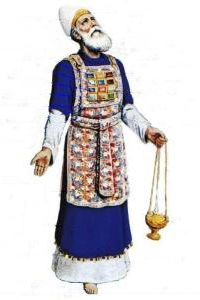
\includegraphics[width=50mm,scale=1.5]{Extras/Melchisedec.jpg}
\vspace{0.4in}  % Create a title for the document and write it in bold font
\LARGE{\textbf{\date}} % Again, do a line break
\linebreak 
% Create a subtitle \large{with Outlines, Statistics, Cross References, and Notes}
\vspace{0.5in}
\begin{flushleft}
\LARGE{Day \#49: Friday, 18 February 2022  \\}\vspace{0.25in}
\LARGE{Numbers 25-27 Psalm 49 Proverb 18}
\end{flushleft}
\vspace{0.6in}
\bigskip

\normalsize{Xenia, Oh.\\}
\normalsize{created: \today}
\vspace{1.3in}

\end{flushright}
\end{titlepage}

\newpage 
\tableofcontents\hypertarget{TOC}{}
\listoffigures
\listoftables

\hyphenation{A-bim-e-lech bre-thren E-phra-im  Gib-e-o-nites Jer-u-sa-lem through-out Phil-i-stines The-o-phil-us Am-a-le-kites ven-geance Mesh-el-e-mi-ah onan-ism Phar-a-oh thoughts grev-ous-ness Hach-a-liah adul-ter-er Shad-rach}

%%%%%%%%%%%%%%%%% EXTRA COLORS
%%%%%%%%%%%%%%%%% EXTRA COLORS
%%%%%%%%%%%%%%%%% EXTRA COLORS
\definecolor{champagne}{rgb}{0.97,0.91,0.81}
\definecolor{bone}{rgb}{0.89,0.85,0.79}

\definecolor{ForestGreen}{rgb}{0.00,0.29,0.098}
\definecolor{GIVING}{cmyk}{1,0.0,0.72,.1}

\definecolor{MLPE}{cmyk}{1,1,0,.45}
\definecolor{SOCCER}{cmyk}{.77, 0, .42, .49}
\definecolor{PAYBILL}{cmyk}{0,0.83,0.76,0.07}
\definecolor{SERMON}{cmyk}{.14,.9,0,.30} % aka seance \href{http://www.flatuicolorpicker.com/purple-cmyk-color-model/}{seance}
\definecolor{BIBLE}{cmyk}{0,.17,.74,.17}
\definecolor{WORKBLUE}{cmyk}{1, .5, 0, .6}
\definecolor{myOrange}{cmyk}{0, .4, .98, .03}
\definecolor{myTan}{cmyk}{0.0,.07,.17,.10}
\definecolor{myRed}{cmyk}{0,1,1,0}
\definecolor{myWhite}{cmyk}{0,0,0,0}
\definecolor{BLUESoD}{cmyk}{.97,.84,0,.04}
\definecolor{WHITE}{cmyk}{0,0,0,0}
\definecolor{OLDGOLD}{cmyk}{0.05,0.3,1.00,0}
\definecolor{CASTLETON}{cmyk}{1,0,0.31,0.66}
\definecolor{cadmiumgreen}{rgb}{0.0, 0.42, 0.24}
\definecolor{jungle}{rgb}{0.203,0.4882,0.1718}
\definecolor{MYGOLD}{rgb}{1,.84,0}

\definecolor{MYLIGHTGRAY}{rgb}{.85,.85,.85}

\definecolor{codegreen}{rgb}{0,0.6,0}
\definecolor{codegray}{rgb}{0.5,0.5,0.5}
\definecolor{codepurple}{rgb}{0.58,0,0.82}
\definecolor{backcolour}{rgb}{0.95,0.95,0.92}


\mdfdefinestyle{MyFrame}{%
    linecolor=blue,
    outerlinewidth=2pt,
    roundcorner=5pt,
    innertopmargin=\baselineskip,
    innerbottommargin=\baselineskip,
    innerrightmargin=10pt,
    innerleftmargin=10pt,
    backgroundcolor=gray!25!white}


\mdfdefinestyle{MyFrame2}{%
    linecolor=black,
    outerlinewidth=2pt,
    roundcorner=5pt,
    innertopmargin=\baselineskip,
    innerbottommargin=\baselineskip,
    innerrightmargin=10pt,
    innerleftmargin=10pt,
    backgroundcolor=yellow!25!white}


%%%%%
%% for PFTTIS list
%%%%%

%%% And Joseph said unto
\index[PFTTIS]{And Joseph said unto!Genesis!Gen 40:008}
\index[PFTTIS]{And Joseph said unto!Genesis!Gen 40:012}
\index[PFTTIS]{And Joseph said unto!Genesis!Gen 41:025}
\index[PFTTIS]{And Joseph said unto!Genesis!Gen 42:014}
\index[PFTTIS]{And Joseph said unto!Genesis!Gen 42:018}
\index[PFTTIS]{And Joseph said unto!Genesis!Gen 44:015}
\index[PFTTIS]{And Joseph said unto!Genesis!Gen 45:003}
\index[PFTTIS]{And Joseph said unto!Genesis!Gen 45:004}
\index[PFTTIS]{And Joseph said unto!Genesis!Gen 46:031}
\index[PFTTIS]{And Joseph said unto!Genesis!Gen 48:009}
\index[PFTTIS]{And Joseph said unto!Genesis!Gen 48:018}
\index[PFTTIS]{And Joseph said unto!Genesis!Gen 50:019}
\index[PFTTIS]{And Joseph said unto!Genesis!Gen 50:024}


%%% a shadow
\index[PFTTIS]{a shadow!1Chronicles!1Chr 029:15}
\index[PFTTIS]{a shadow!Job!Job 008:09}
\index[PFTTIS]{a shadow!Job!Job 014:02}
\index[PFTTIS]{a shadow!Job!Job 017:07}
\index[PFTTIS]{a shadow!Psalm!Psa 102:011}
\index[PFTTIS]{a shadow!Psalm!Psa 144:004}
\index[PFTTIS]{a shadow!Ecclesiastes!Eccl 006:012}
\index[PFTTIS]{a shadow!Ecclesiastes!Eccl 008:013}
\index[PFTTIS]{a shadow!Isaiah!Isa 04:006}
\index[PFTTIS]{a shadow!Isaiah!Isa 25:004}
\index[PFTTIS]{a shadow!Jonah!Jnh 04:06}
\index[PFTTIS]{a shadow!Colossians!Col 02:017}
\index[PFTTIS]{a shadow!Hebews!Heb 10:001}

%%% blessed is the man
\index[PFTTIS]{blessed is the man!Psalm!Psa 001:001}
\index[PFTTIS]{blessed is the man!Psalm!Psa 032:002}
\index[PFTTIS]{blessed is the man!Psalm!Psa 034:008}
\index[PFTTIS]{blessed is the man!Psalm!Psa 065:004}
\index[PFTTIS]{blessed is the man!Psalm!Psa 084:005}
\index[PFTTIS]{blessed is the man!Psalm!Psa 084:012}
\index[PFTTIS]{blessed is the man!Psalm!Psa 094:012}
\index[PFTTIS]{blessed is the man!Psalm!Psa 112:001}
\index[PFTTIS]{blessed is the man!Proverbs!Pro 008:034}
\index[PFTTIS]{blessed is the man!Isaiah!Isa 056:002}
\index[PFTTIS]{blessed is the man!Jeremiah!Jer 017:007}
\index[PFTTIS]{blessed is the man!Romans!Rom 004:008}
\index[PFTTIS]{blessed is the man!James!Jam 001:012}


%%% carry them
\index[PFTTIS]{carry them!Leviticus!Lev 14:045}
\index[PFTTIS]{carry them!Numbers!Num 11:012}
\index[PFTTIS]{carry them!Joshua!Jsh 04:003}
\index[PFTTIS]{carry them!1Samuel!1Sam 20:040}
\index[PFTTIS]{carry them!1Kings!1Kng 08:046}
\index[PFTTIS]{carry them!2Chronicles!2Chr 06:036}
\index[PFTTIS]{carry them!Ezra!Ezra 05:015}
\index[PFTTIS]{carry them!Isaiah!Isa 40:011}
\index[PFTTIS]{carry them!Isaiah!Isa 41:016}
\index[PFTTIS]{carry them!Isaiah!Isa 57:013}
\index[PFTTIS]{carry them!Jeremiah!Jer 20:004}
\index[PFTTIS]{carry them!Jeremiah!Jer 20:005}
\index[PFTTIS]{carry them!Jeremiah!Jer 43:012}


\index[PFTTIS]{good tidings!2Samuel!2Sam 18:027}
\index[PFTTIS]{good tidings!1Kings!1Ki 01:042}
\index[PFTTIS]{good tidings!2Kings!2Ki 07:009 (2x)}
\index[PFTTIS]{good tidings!Isaiah!Isa 40:009 (2x)}
\index[PFTTIS]{good tidings!Isaiah!Isa 41:007}
\index[PFTTIS]{good tidings!Isaiah!Isa 52:007}
\index[PFTTIS]{good tidings!Isaiah!Isa 61:001}
\index[PFTTIS]{good tidings!Nahum!Nah 01:005}
\index[PFTTIS]{good tidings!Luke!Lk 02:010}
\index[PFTTIS]{good tidings!1Thessalonians!1Thess 03:006}


%%% dead body
\index[PFTTIS]{dead body!Leviticus!Lev 21:011}
\index[PFTTIS]{dead body!Numbers!Num 06:006}
\index[PFTTIS]{dead body!Numbers!Num 09:006}
\index[PFTTIS]{dead body!Numbers!Num 09:007}
\index[PFTTIS]{dead body!Numbers!Num 09:010}
\index[PFTTIS]{dead body!Numbers!Num 09:011}
\index[PFTTIS]{dead body!Numbers!Num 09:013}
\index[PFTTIS]{dead body!Numbers!Num 09:016}
\index[PFTTIS]{dead body!2Kings!2Ki 08:005}
\index[PFTTIS]{dead body!Isaiah!Isa 26:019}
\index[PFTTIS]{dead body!Jeremiah!Jer 26:023}
\index[PFTTIS]{dead body!Jeremiah!Jer 36:030}
\index[PFTTIS]{dead body!Haggai!Hag 02:013}

%%% great sea
\index[PFTTIS]{great sea!Numbers!Num 34:006}
\index[PFTTIS]{great sea!Numbers!Num 34:007}
\index[PFTTIS]{great sea!Joshua!Jos 01:004}
\index[PFTTIS]{great sea!Joshua!Jos 09:001}
\index[PFTTIS]{great sea!Joshua!Jos 15:012}
\index[PFTTIS]{great sea!Joshua!Jos 15:047}
\index[PFTTIS]{great sea!Joshua!Jos 23:004}
\index[PFTTIS]{great sea!Ezekiel!Eze 47:010}
\index[PFTTIS]{great sea!Ezekiel!Eze 47:015}
\index[PFTTIS]{great sea!Ezekiel!Eze 47:019}
\index[PFTTIS]{great sea!Ezekiel!Eze 47:020}
\index[PFTTIS]{great sea!Ezekiel!Eze 48:028}
\index[PFTTIS]{great sea!Daniel!Dan 07:002}


%%% have forsaken me
\index[PFTTIS]{have forsaken me!Judges!Jdg 10:013}
\index[PFTTIS]{have forsaken me!1Samuel!1Sam 08:008}
\index[PFTTIS]{have forsaken me!1Kings!1Ki 11:033}
\index[PFTTIS]{have forsaken me!2Kings!2Ki 22:017}
\index[PFTTIS]{have forsaken me!2Chronicles!2Chr 12:005}
\index[PFTTIS]{have forsaken me!2Chronicles!2Chr 34:025}
\index[PFTTIS]{have forsaken me!Jeremiah!Jer 01:016}
\index[PFTTIS]{have forsaken me!Jeremiah!Jer 02:013}
\index[PFTTIS]{have forsaken me!Jeremiah!Jer 05:007}
\index[PFTTIS]{have forsaken me!Jeremiah!Jer 05:019}
\index[PFTTIS]{have forsaken me!Jeremiah!Jer 16:011 (2x)}
\index[PFTTIS]{have forsaken me!Jeremiah!Jer 19:004}

%%% no king
\index[PFTTIS]{no king!Judges!Jdg 17:06}
\index[PFTTIS]{no king!Judges!Jdg 18:01}
\index[PFTTIS]{no king!Judges!Jdg 19:01}
\index[PFTTIS]{no king!Judges!Jdg 21:25}
\index[PFTTIS]{no king!1Kings!1Ki 22:47}
\index[PFTTIS]{no king!2Kings!2Ki 23:25}
\index[PFTTIS]{no king!Nehemiah!Neh 13:26}
\index[PFTTIS]{no king!Psalms!Psa 033:016}
\index[PFTTIS]{no king!Proverbs!Pro 30:27}
\index[PFTTIS]{no king!Daniel!Dan 02:10}
\index[PFTTIS]{no king!Hosea!Hos 10:03}
\index[PFTTIS]{no king!Micah!Mic 04:09}
\index[PFTTIS]{no king!John!Jhn 19:15}


%%% rebellious house
\index[PFTTIS]{rebellious house!Exodus!Exo 02:005}
\index[PFTTIS]{rebellious house!Exodus!Exo 02:006}
\index[PFTTIS]{rebellious house!Exodus!Exo 02:008}
\index[PFTTIS]{rebellious house!Exodus!Exo 03:009}
\index[PFTTIS]{rebellious house!Exodus!Exo 03:026}
\index[PFTTIS]{rebellious house!Exodus!Exo 03:027}
\index[PFTTIS]{rebellious house!Exodus!Exo 12:002 (2x)}
\index[PFTTIS]{rebellious house!Exodus!Exo 12:003}
\index[PFTTIS]{rebellious house!Exodus!Exo 12:009}
\index[PFTTIS]{rebellious house!Exodus!Exo 12:025}
\index[PFTTIS]{rebellious house!Exodus!Exo 17:012}
\index[PFTTIS]{rebellious house!Exodus!Exo 24:003}

%%% seek him
\index[PFTTIS]{seek him!Deuteronomy!Deu 04:029}\index[PFTTIS]{seek him!1Samuel!1Sam 23:025}
\index[PFTTIS]{seek him!1Chronicles!1Chr 28:009}
\index[PFTTIS]{seek him!2Chronicles!1Chr 15:002}
\index[PFTTIS]{seek him!Ezra!Ezr 08:022}
\index[PFTTIS]{seek him!Psalms!Psa 022:026}
\index[PFTTIS]{seek him!Psalms!Psa 024:006}
\index[PFTTIS]{seek him!Psalms!Psa 119:002}
\index[PFTTIS]{seek him!SoS!SoS 03:002}
\index[PFTTIS]{seek him!SoS!SoS 06:001}
\index[PFTTIS]{seek him!Hosea!Hos 07:010}
\index[PFTTIS]{seek him!Amos!Amo 05:008}
\index[PFTTIS]{seek him!Hebrews!Heb 11:0063}


%%% seek ye
\index[PFTTIS]{seek ye!Isaiah!Isa 34:016}
\index[PFTTIS]{seek ye!Isaiah!Isa 45:019}
\index[PFTTIS]{seek ye!Isaiah!Isa 55:006}
\index[PFTTIS]{seek ye!Amos!Amos 5:004}
\index[PFTTIS]{seek ye!John!John 1:38}
\index[PFTTIS]{seek ye!John!John 18:4}
\index[PFTTIS]{seek ye!John!John 18:7}
\index[PFTTIS]{seek ye!Matthew!Matt 6:33}
\index[PFTTIS]{seek ye!Numbers!Num 16:10}
\index[PFTTIS]{seek ye!Luke!Luke 12:31}
\index[PFTTIS]{seek ye!Luke!Luke 24:5}
\index[PFTTIS]{seek ye!Psalm!Psa 27:8}
\index[PFTTIS]{seek ye!Zephaniah!Zeph 2:3}

%%% the uncircumcised
\index[PFTTIS]{the uncircumcised!Genesis!Gen 17:014}
\index[PFTTIS]{the uncircumcised!Judges!Jdg 14:003}
\index[PFTTIS]{the uncircumcised!Judges!Jdg 15:018}
\index[PFTTIS]{the uncircumcised!2Samuel!2Sam 01:020}
\index[PFTTIS]{the uncircumcised!Isaiah!Isa 02:001}
\index[PFTTIS]{the uncircumcised!Jeremiah!Jer 09:025}
\index[PFTTIS]{the uncircumcised!Ezekiel!Eze 28:010}
\index[PFTTIS]{the uncircumcised!Ezekiel!Eze 31:018}
\index[PFTTIS]{the uncircumcised!Ezekiel!Eze 32:019}
\index[PFTTIS]{the uncircumcised!Ezekiel!Eze 32:027}
\index[PFTTIS]{the uncircumcised!Ezekiel!Eze 32:028}
\index[PFTTIS]{the uncircumcised!Ezekiel!Eze 32:029}
\index[PFTTIS]{the uncircumcised!Ezekiel!Eze 32:032}

%%% worship him
\index[PFTTIS]{worship him!Psalms!Psa 97:007}
\index[PFTTIS]{worship him!Zephaniah!Zeph 02:011}
\index[PFTTIS]{worship him!Matthew!Matt 02:002}
\index[PFTTIS]{worship him!Matthew!Matt 02:008}
\index[PFTTIS]{worship him!John!John 04:023}
\index[PFTTIS]{worship him!John!John 04:024 (2x)} 
\index[PFTTIS]{worship him!Acts!Acts 17:023}
\index[PFTTIS]{worship him!Hebrews!Heb 01:006}
\index[PFTTIS]{worship him!Revelation!Rev 04:010}
\index[PFTTIS]{worship him!Revelation!Rev 13:008}
\index[PFTTIS]{worship him!Revelation!Rev 14:007}
\index[PFTTIS]{worship him!Revelation!Rev 19:010}


%%%%%
%% for PFTTIS list
%%%%%

%%% afflictions
\index[WFTTIS]{afflictions!Psalms!Psa 34:019}
\index[WFTTIS]{afflictions!Psalms!Psa 132:001}
\index[WFTTIS]{afflictions!Acts!Acts 07:010}
\index[WFTTIS]{afflictions!Acts!Acts 20:023}
\index[WFTTIS]{afflictions!2Corinthians!2Cor 06:004}
\index[WFTTIS]{afflictions!Colossians!Col 01:024}
\index[WFTTIS]{afflictions!1Thessalonians!1Thess 03:003}
\index[WFTTIS]{afflictions!2Timothy!2Tim 01:008}
\index[WFTTIS]{afflictions!2Timothy!2Tim 03:011}
\index[WFTTIS]{afflictions!2Timothy!2Tim 04:005}
\index[WFTTIS]{afflictions!Hebrews!Heb 10:032}
\index[WFTTIS]{afflictions!Hebrews!Heb 10:033}
\index[WFTTIS]{afflictions!1Peter!1Pet 05:009}

%%% acsend
\index[WFTTIS]{acsend!Joshua!Jos 06:05}
\index[WFTTIS]{acsend!Psalm!Psa 024:003}
\index[WFTTIS]{acsend!Psalm!Psa 135:007}
\index[WFTTIS]{acsend!Psalm!Psa 139:008}
\index[WFTTIS]{acsend!Isaiah!Isa 14:013}
\index[WFTTIS]{acsend!Isaiah!Isa 14:014}
\index[WFTTIS]{acsend!Jeremiah!Jer 10:013}
\index[WFTTIS]{acsend!Jeremiah!Jer 51:016}
\index[WFTTIS]{acsend!Ezekiel!Eze 38:009}
\index[WFTTIS]{acsend!John!John 06:062}
\index[WFTTIS]{acsend!John!John 20:017}
\index[WFTTIS]{acsend!Romans!Rom 10:006}
\index[WFTTIS]{acsend!Revelation!Rev 17:008}

%%% Assyrian
\index[WFTTIS]{Assyrian!Isaiah!Isa 10:005}
\index[WFTTIS]{Assyrian!Isaiah!Isa 10:024}
\index[WFTTIS]{Assyrian!Isaiah!Isa 14:025}
\index[WFTTIS]{Assyrian!Isaiah!Isa 19:023}
\index[WFTTIS]{Assyrian!Isaiah!Isa 23:013}
\index[WFTTIS]{Assyrian!Isaiah!Isa 30:031}
\index[WFTTIS]{Assyrian!Isaiah!Isa 31:008}
\index[WFTTIS]{Assyrian!Isaiah!Isa 52:004}
\index[WFTTIS]{Assyrian!Ezekiel!Eze 31:003}
\index[WFTTIS]{Assyrian!Hosea!Hos 05:013}
\index[WFTTIS]{Assyrian!Hosea!Hos 11:005}
\index[WFTTIS]{Assyrian!Micah!Hos 05:005}
\index[WFTTIS]{Assyrian!Micah!Hos 05:006}

%%% blot
\index[WFTTIS]{blot!Exodus!Exo 32:032}
\index[WFTTIS]{blot!Exodus!Exo 32:033}
\index[WFTTIS]{blot!Numbers!Num 05:026}
\index[WFTTIS]{blot!Deuteronomy!Deut 09:014}
\index[WFTTIS]{blot!Deuteronomy!Deut 25:019}
\index[WFTTIS]{blot!Deuteronomy!Deut 29:020}
\index[WFTTIS]{blot!2Kings!2Ki 14:027}
\index[WFTTIS]{blot!Job!Job 31:007}
\index[WFTTIS]{blot!Psalms!Psa 51:001}
\index[WFTTIS]{blot!Psalms!Psa 51:009}
\index[WFTTIS]{blot!Proverbs!Pro 09:007}
\index[WFTTIS]{blot!Jeremiah!Jer 18:023}
\index[WFTTIS]{blot!Revelation!Rev 03:005}


%%% chain
\index[WFTTIS]{chain!Genesis!Gen 41:042}
\index[WFTTIS]{chain!1Kings!1Ki 07:017}
\index[WFTTIS]{chain!Psalms!Psa 73:006}
\index[WFTTIS]{chain!SoS!Sos 04:009}
\index[WFTTIS]{chain!Lamentations!Lam 03:007}
\index[WFTTIS]{chain!Ezekiel!Eze 07:023}
\index[WFTTIS]{chain!Ezekiel!Eze 16:011}
\index[WFTTIS]{chain!Daniel!Dan 05:007}
\index[WFTTIS]{chain!Daniel!Dan 05:016}
\index[WFTTIS]{chain!Daniel!Dan 05:029}
\index[WFTTIS]{chain!Acts!Acts 28:020}
\index[WFTTIS]{chain!2Timothy!2Tim 01:016}
\index[WFTTIS]{chain!Revelation!Rev 20:001}


%%% controversy
\index[WFTTIS]{controversy!Deuteronomy!Deu 17:008}
\index[WFTTIS]{controversy!Deuteronomy!Deu 19:017}
\index[WFTTIS]{controversy!Deuteronomy!Deu 21:005}
\index[WFTTIS]{controversy!Deuteronomy!Deu 25:001}
\index[WFTTIS]{controversy!2Samuel!2Sam 15:002}
\index[WFTTIS]{controversy!Isaiah!Isa 34:008}
\index[WFTTIS]{controversy!Jeremiah!Jer 25:031}
\index[WFTTIS]{controversy!Ezekiel!Eze 44:024}
\index[WFTTIS]{controversy!Hosea!Hos 04:001}
\index[WFTTIS]{controversy!Hosea!Hos 12:002}
\index[WFTTIS]{controversy!Micah!Mic 06:002 (2x)}
\index[WFTTIS]{controversy!1Timothy!1Tim 03:016}


%%% Dagon/Dagon's
\index[WFTTIS]{Dagon!Judges!Jdg 16:023}
\index[WFTTIS]{Dagon!1Samuel!1Sam 05:002 (2x)}
\index[WFTTIS]{Dagon!1Samuel!1Sam 05:003 (2x)}
\index[WFTTIS]{Dagon!1Samuel!1Sam 05:004 (3x)}
\index[WFTTIS]{Dagon!1Samuel!1Sam 05:005 (3x)}
\index[WFTTIS]{Dagon!1Samuel!1Sam 05:007}
\index[WFTTIS]{Dagon!1Chronicles!1Chr 10:010}

%%% disobedient
\index[WFTTIS]{disobedient!1Kings!1Ki 13:026}
\index[WFTTIS]{disobedient!Nehemiah!Neh 09:026}
\index[WFTTIS]{disobedient!Luke!Luke 01:017}
\index[WFTTIS]{disobedient!Acts!Acts 26:019}
\index[WFTTIS]{disobedient!Romans!Rom 01:030}
\index[WFTTIS]{disobedient!Romans!Rom 10:021}
\index[WFTTIS]{disobedient!1Timothy!1Tim 01:009}
\index[WFTTIS]{disobedient!2Timothy!2Tim 03:002}
\index[WFTTIS]{disobedient!Titus!Titus 01:016}
\index[WFTTIS]{disobedient!Titus!Titus 03:003}
\index[WFTTIS]{disobedient!1Peter!1Pet 02:007}
\index[WFTTIS]{disobedient!1Peter!1Pet 02:008}
\index[WFTTIS]{disobedient!1Peter!1Pet 03:020}


%%% doubt
\index[WFTTIS]{doubt!Genesis!Gen 37:033}
\index[WFTTIS]{doubt!Deuteronomy!Deu 28:066}
\index[WFTTIS]{doubt!Job!Job 12:002}
\index[WFTTIS]{doubt!Matthew!Matt 14:031}
\index[WFTTIS]{doubt!Matthew!Matt 21:021}
\index[WFTTIS]{doubt!Mark!Mk 11:023}
\index[WFTTIS]{doubt!Luke!Lk 11:020}
\index[WFTTIS]{doubt!John!Jhn 10:024}
\index[WFTTIS]{doubt!Acts!Acts 02:012}
\index[WFTTIS]{doubt!Acts!Acts 28:004}
\index[WFTTIS]{doubt!1Corinthians!1Cor 09:010}
\index[WFTTIS]{doubt!Galatians!Gal 04:020}
\index[WFTTIS]{doubt!1John!1Jhn 02:019}


%%% dungeon
\index[WFTTIS]{dungeon!Genesis!Gen 40:015}
\index[WFTTIS]{dungeon!Genesis!Gen 41:014}
\index[WFTTIS]{dungeon!Exodus!Exo 12:029}
\index[WFTTIS]{dungeon!Jeremiah!Jer 37:016}
\index[WFTTIS]{dungeon!Jeremiah!Jer 38:006 (2x)}
\index[WFTTIS]{dungeon!Jeremiah!Jer 38:007}
\index[WFTTIS]{dungeon!Jeremiah!Jer 38:009}
\index[WFTTIS]{dungeon!Jeremiah!Jer 38:010}
\index[WFTTIS]{dungeon!Jeremiah!Jer 38:011}
\index[WFTTIS]{dungeon!Jeremiah!Jer 38:013}
\index[WFTTIS]{dungeon!Lamentations!Lam 03:053}
\index[WFTTIS]{dungeon!Lamentations!Lam 03:055}


%%% error
\index[WFTTIS]{error!2Samuel!2Sam 06:007}
\index[WFTTIS]{error!Job!Job 19:004}
\index[WFTTIS]{error!Ecclesiastes!Ecc 05:006}
\index[WFTTIS]{error!Ecclesiastes!Ecc 10:005}
\index[WFTTIS]{error!Isaiah!Isa 32:006}
\index[WFTTIS]{error!Daniel!Dan 06:004}
\index[WFTTIS]{error!Matthew!Matt 27:064}
\index[WFTTIS]{error!Romans!Rom 01:027}
\index[WFTTIS]{error!James!Jam 05:020}
\index[WFTTIS]{error!2Peter!2Pet 02:018}
\index[WFTTIS]{error!2Peter!2Pet 03:017}
\index[WFTTIS]{error!1John!1Jn 04:006}
\index[WFTTIS]{error!Jude!Jude 01:011}

%%% fourish
\index[WFTTIS]{fourish!Psalms!Psa 072:007}
\index[WFTTIS]{fourish!Psalms!Psa 072:016}
\index[WFTTIS]{fourish!Psalms!Psa 092:007}
\index[WFTTIS]{fourish!Psalms!Psa 092:012}
\index[WFTTIS]{fourish!Psalms!Psa 092:013}
\index[WFTTIS]{fourish!Psalms!Psa 132:018}
\index[WFTTIS]{fourish!Proverbs!Pro 11:28}
\index[WFTTIS]{fourish!Proverbs!Pro 14:11}
\index[WFTTIS]{fourish!Ecclesiastes!Ecc 12:05}
\index[WFTTIS]{fourish!SongOfSolomon!SOS 07:12}
\index[WFTTIS]{fourish!Isaiah!Isa 17:11}
\index[WFTTIS]{fourish!Isaiah!Isa 66:14}
\index[WFTTIS]{fourish!Ezekiel!Eze 17:24}




%%% giants
\index[WFTTIS]{giants!Genesis!Gen 06:004}
\index[WFTTIS]{giants!Numbers!Num 13:033}
\index[WFTTIS]{giants!Deuteronomy!Deut 02:011}
\index[WFTTIS]{giants!Deuteronomy!Deut 02:021}
\index[WFTTIS]{giants!Deuteronomy!Deut 03:011}
\index[WFTTIS]{giants!Deuteronomy!Deut 03:013}
\index[WFTTIS]{giants!Joshua!Josh 12:004}
\index[WFTTIS]{giants!Joshua!Josh 13:012}
\index[WFTTIS]{giants!Joshua!Josh 15:008}
\index[WFTTIS]{giants!Joshua!Josh 17:015}
\index[WFTTIS]{giants!Joshua!Josh 16:016}

%%% good man
\index[WFTTIS]{good man!2 Samuel!2Sa 18:27}
%(1) Psalms 37:23 [5]
%(1) Psalms 112:5 [2]
%(1) Proverbs 12:2 [2]
%(1) Proverbs 13:22 [2]
%(1) Proverbs 14:14 [14]
%(1) Micah 7:2 [2]
%(1) Matthew 12:35 [2]
%(1) Luke 6:45 [2]
%(1) Luke 23:50 [15]
%(1) John 7:12 [17]
%(1) Acts 11:24 [5]
%(1) Romans 5:7 [14]

%%% Hinnom
\index[WFTTIS]{Hinnom!Joshua!Jsh 15:008}
\index[WFTTIS]{Hinnom!Joshua!Jsh 18:016}
\index[WFTTIS]{Hinnom!2Kings!2Ki 23:010}
\index[WFTTIS]{Hinnom!2Chronicles!2Chr 28:003}
\index[WFTTIS]{Hinnom!2Chronicles!2Chr 33:006}
\index[WFTTIS]{Hinnom!Nehemiah!Neh 11:030}
\index[WFTTIS]{Hinnom!Jeremiah!Jer 07:031}
\index[WFTTIS]{Hinnom!Jeremiah!Jer 07:032}
\index[WFTTIS]{Hinnom!Jeremiah!Jer 19:002}
\index[WFTTIS]{Hinnom!Jeremiah!Jer 19:006}
\index[WFTTIS]{Hinnom!Jeremiah!Jer 32:035}

%%% inclined
\index[WFTTIS]{inclined!Judges!Jdg 09:003}
\index[WFTTIS]{inclined!Psalms!Psa 040:001}
\index[WFTTIS]{inclined!Psalms!Psa 116:002}
\index[WFTTIS]{inclined!Psalms!Psa 119:112}
\index[WFTTIS]{inclined!Proverbs!Pro 05:13}
\index[WFTTIS]{inclined!Jeremiah!Jer 07:24}
\index[WFTTIS]{inclined!Jeremiah!Jer 07:26}
\index[WFTTIS]{inclined!Jeremiah!Jer 11:08}
\index[WFTTIS]{inclined!Jeremiah!Jer 17:23}
\index[WFTTIS]{inclined!Jeremiah!Jer 25:04}
\index[WFTTIS]{inclined!Jeremiah!Jer 34:14}
\index[WFTTIS]{inclined!Jeremiah!Jer 35:15}
\index[WFTTIS]{inclined!Jeremiah!Jer 44:05}


%%% laughed
\index[WFTTIS]{laughed!Genesis!Gen 17:017}
\index[WFTTIS]{laughed!Genesis!Gen 18:012}
\index[WFTTIS]{laughed!Genesis!Gen 18:015}
\index[WFTTIS]{laughed!2Kings!2Ki 19:021}
\index[WFTTIS]{laughed!2Chronicles!2Chr 30:010}
\index[WFTTIS]{laughed!Nehemiah!Neh 02:019}
\index[WFTTIS]{laughed!Job!Job 12:004}
\index[WFTTIS]{laughed!Job!Job 29:024}
\index[WFTTIS]{laughed!Isaiah!Isa 37:022}
\index[WFTTIS]{laughed!Ezekiel!Ezek 23:032}
\index[WFTTIS]{laughed!Matthew!Matt 09:024}
\index[WFTTIS]{laughed!Mark!Mk 05:040}
\index[WFTTIS]{laughed!Luke!Lk 08:053}

%%% liar
\index[WFTTIS]{liar!Job!Job 24:025}
\index[WFTTIS]{liar!Proverbs!Pro 17:004}
\index[WFTTIS]{liar!Proverbs!Pro 19:022}
\index[WFTTIS]{liar!Proverbs!Pro 30:006}
\index[WFTTIS]{liar!Jeremiah!Jer 15:018}
\index[WFTTIS]{liar!John!Jhn 08:044}
\index[WFTTIS]{liar!John!Jhn 08:055}
\index[WFTTIS]{liar!Romans!Rom 03:004}
\index[WFTTIS]{liar!1John!1Jhn 01:010}
\index[WFTTIS]{liar!1John!1Jhn 02:004}
\index[WFTTIS]{liar!1John!1Jhn 02:022}
\index[WFTTIS]{liar!1John!1Jhn 04:020}
\index[WFTTIS]{liar!1John!1Jhn 05:010}

%%% palsy
\index[WFTTIS]{palsy!Matthew!Matt 04:024}
\index[WFTTIS]{palsy!Matthew!Matt 08:006}
\index[WFTTIS]{palsy!Matthew!Matt 09:002}
\index[WFTTIS]{palsy!Matthew!Matt 09:006}
\index[WFTTIS]{palsy!Mark!Mk 02:003}
\index[WFTTIS]{palsy!Mark!Mk 02:004}
\index[WFTTIS]{palsy!Mark!Mk 02:005}
\index[WFTTIS]{palsy!Mark!Mk 02:009}
\index[WFTTIS]{palsy!Mark!Mk 02:010}
\index[WFTTIS]{palsy!Luke!Lk 05:018}
\index[WFTTIS]{palsy!Luke!Lk 05:024}
\index[WFTTIS]{palsy!Acts!Acts 09:033}

%%% Profitable
\index[WFTTIS]{profitable!Job!Job 22:002 (2x)}
\index[WFTTIS]{profitable!Ecclesiastes!Ecc 10:010}
\index[WFTTIS]{profitable!Isaiah!Isa 44:010}
\index[WFTTIS]{profitable!Jeremiah!Jer 13:007}
\index[WFTTIS]{profitable!Matthew!Matt 05:029}
\index[WFTTIS]{profitable!Matthew!Matt 05:030}
\index[WFTTIS]{profitable!Acts!Acts 20:020}
\index[WFTTIS]{profitable!1Timothy!1Tim 04:008}
\index[WFTTIS]{profitable!2Timothy!2Tim 03:016}
\index[WFTTIS]{profitable!2Timothy!2Tim 04:011}
\index[WFTTIS]{profitable!Titus!Titus 03:008}
\index[WFTTIS]{profitable!Philemon!Phlm 01:011}

%%% Rechab
\index[WFTTIS]{Rechab!2Samuel!2Sam 04:002}
\index[WFTTIS]{Rechab!2Samuel!2Sam 04:005}
\index[WFTTIS]{Rechab!2Samuel!2Sam 04:006}
\index[WFTTIS]{Rechab!2Samuel!2Sam 04:009}
\index[WFTTIS]{Rechab!2KIngs!2Ki 10:015}
\index[WFTTIS]{Rechab!2KIngs!2Ki 10:023}
\index[WFTTIS]{Rechab!1Chronicles!1Chr 02:055}
\index[WFTTIS]{Rechab!Nehemiah!Neh 03:014}
\index[WFTTIS]{Rechab!Jeremiah!Jer 35:006}
\index[WFTTIS]{Rechab!Jeremiah!Jer 35:008}
\index[WFTTIS]{Rechab!Jeremiah!Jer 35:014}
\index[WFTTIS]{Rechab!Jeremiah!Jer 35:016}
\index[WFTTIS]{Rechab!Jeremiah!Jer 35:019}

%%% serpents
\index[WFTTIS]{serpents!Exodus!Exo 07:012}
\index[WFTTIS]{serpents!Numbers!Num 21:006}
\index[WFTTIS]{serpents!Numbers!Num 21:007}
\index[WFTTIS]{serpents!Deuteronomy!Deu 08:015}
\index[WFTTIS]{serpents!Deuteronomy!Deu 32:024}
\index[WFTTIS]{serpents!Jeremiah!Jer 08:017}
\index[WFTTIS]{serpents!Matthew!Matt 10:016}
\index[WFTTIS]{serpents!Matthew!Matt 23:033}
\index[WFTTIS]{serpents!Mark!Mk 16:018}
\index[WFTTIS]{serpents!Luke!Lk 10:019}
\index[WFTTIS]{serpents!1Corinthians!1Cor 10:009}
\index[WFTTIS]{serpents!James!Jas 03:007}
\index[WFTTIS]{serpents!Revelation!Rev 09:019}

%%% short
\index[WFTTIS]{short!Numbers!Num 11:023}
\index[WFTTIS]{short!2Kings!2Ki 10:032}
\index[WFTTIS]{short!Job!Job 17:012}
\index[WFTTIS]{short!Job!Job 20:005}
\index[WFTTIS]{short!Psalms!Psa 89:047}
\index[WFTTIS]{short!Romans!Rom 03:023}
\index[WFTTIS]{short!Romans!Rom 09:028  (2x)}
\index[WFTTIS]{short!1Corinthians!1Cor 07:029}
\index[WFTTIS]{short!1Thessalonians!1Thess 02:017}
\index[WFTTIS]{short!Hebrews!Heb 04:001}
\index[WFTTIS]{short!Revelation!Rev 12:012}
\index[WFTTIS]{short!Revelation!Rev 17:010}

%%% smiteth
\index[WFTTIS]{smiteth!Exodus!Exo 21:012}
\index[WFTTIS]{smiteth!Exodus!Exo 21:15}
\index[WFTTIS]{smiteth!Deuteronomy!Dt 25:11}
\index[WFTTIS]{smiteth!Deuteronomy!Dt 27:24}
\index[WFTTIS]{smiteth!Joshua!Jsh 15:16}
\index[WFTTIS]{smiteth!Judges!Jdg 15:16}
\index[WFTTIS]{smiteth!2 Samuel!2Sa 05:08}
\index[WFTTIS]{smiteth!1Chronicles!1Chr 11:06}
\index[WFTTIS]{smiteth!Job!1Chr 26:12}
\index[WFTTIS]{smiteth!Isaiah!Isa 09:13}
\index[WFTTIS]{smiteth!Lamentations!Lam 03:30}
\index[WFTTIS]{smiteth!Ezekiel!Eze 07:09}
\index[WFTTIS]{smiteth!Luke!Lk 06:29}



%%% vanities
\index[WFTTIS]{vanities!Deuteronomy!Deut 21:021}
\index[WFTTIS]{vanities!1Kings!1Ki 16:013}
\index[WFTTIS]{vanities!1Kings!1Ki 16:026}
\index[WFTTIS]{vanities!Psalms!Psa 031:006}
\index[WFTTIS]{vanities!Ecclesiastes!Ecc 01:002 (2x)}
\index[WFTTIS]{vanities!Ecclesiastes!Ecc 05:007}
\index[WFTTIS]{vanities!Ecclesiastes!Ecc 12:008}
\index[WFTTIS]{vanities!Jeremiah!Jer 08:019}
\index[WFTTIS]{vanities!Jeremiah!Jer 10:008}
\index[WFTTIS]{vanities!Jeremiah!Jer 14:022}
\index[WFTTIS]{vanities!Jonah!Jnh 02:008}
\index[WFTTIS]{vanities!Acts!Acts 14:015}



%%%%%
%% for PFTTIS list
%%%%%

%%% worm
\index[WFITV]{worm!Exodus!Exo 16:024}
\index[WFITV]{worm!Job!Job 17:014}
\index[WFITV]{worm!Job!Job 24:029}
\index[WFITV]{worm!Job!Job 25:005 (2x)}
\index[WFITV]{worm!Psalms!Psa 022:006}
\index[WFITV]{worm!Isaiah!Isa 14:011}
\index[WFITV]{worm!Isaiah!Isa 41:014}
\index[WFITV]{worm!Isaiah!Isa 51:008}
\index[WFITV]{worm!Isaiah!Isa 66:024}
\index[WFITV]{worm!Jonah!Jnh 04:007}
\index[WFITV]{worm!Mark!Mk 09:044}
\index[WFITV]{worm!Mark!Mk 09:046}
\index[WFITV]{worm!Mark!Mk 09:048}


%\subsubsection{Title}
%\textbf{Introduction:} Isaiah 46 
%\index[speaker]{Speaker!Isaiah 49 (Title}
%\index[series]{Book (Speaker)!IPassage (Title)}
%\index[date]{2017/07/09!Isaiah 49 (Title)}
%\begin{compactenum}[I.]
%    \item  \textbf{Point} \index[scripture]{Isaiah!IPassage} (IPassage)
%\end{compactenum}




  


%\input{02OT-Exodus/ExodusIntroduction}
\newpage
\begin{figure}
\begin{center}
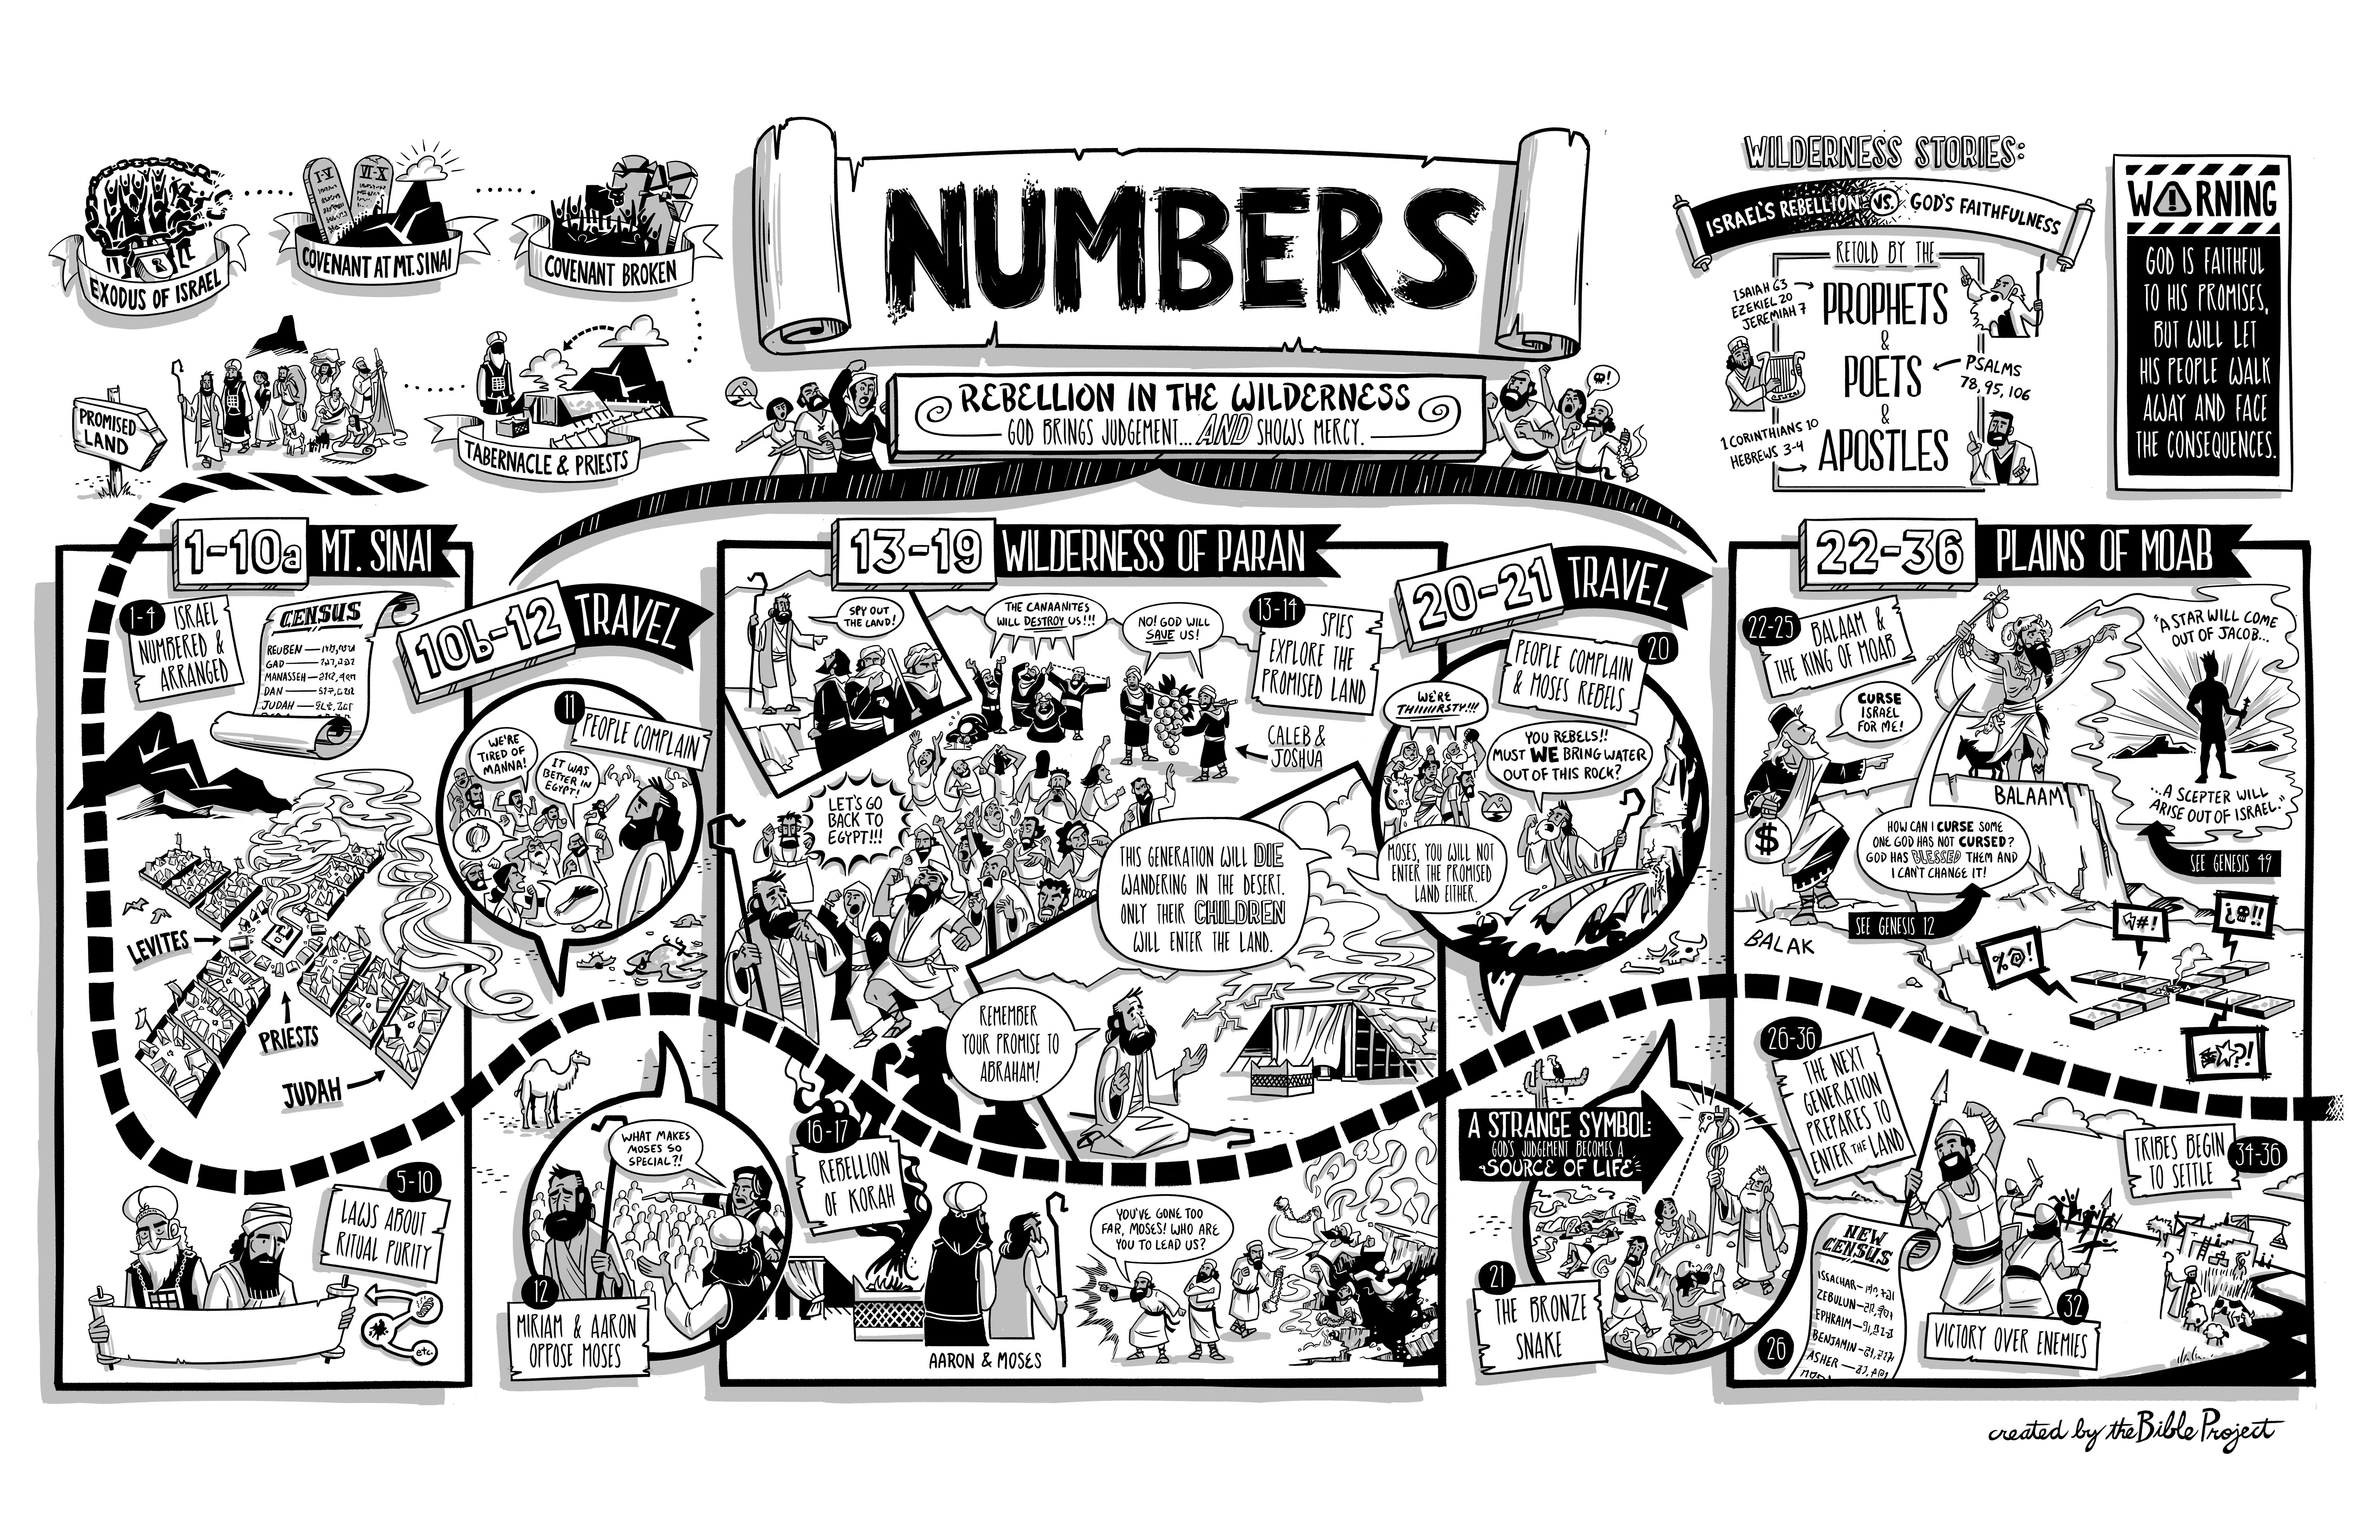
\includegraphics[scale=0.5, angle=90]{04OT-Numbers/References/BibleProject-Numbers.jpg}
\caption[Numbers from the Bible Project]{Numbers from the Bible Project}
\label{fig:Numbers from the Bible Project}
\end{center}
\end{figure}

\newpage
\begin{figure}
\begin{center}
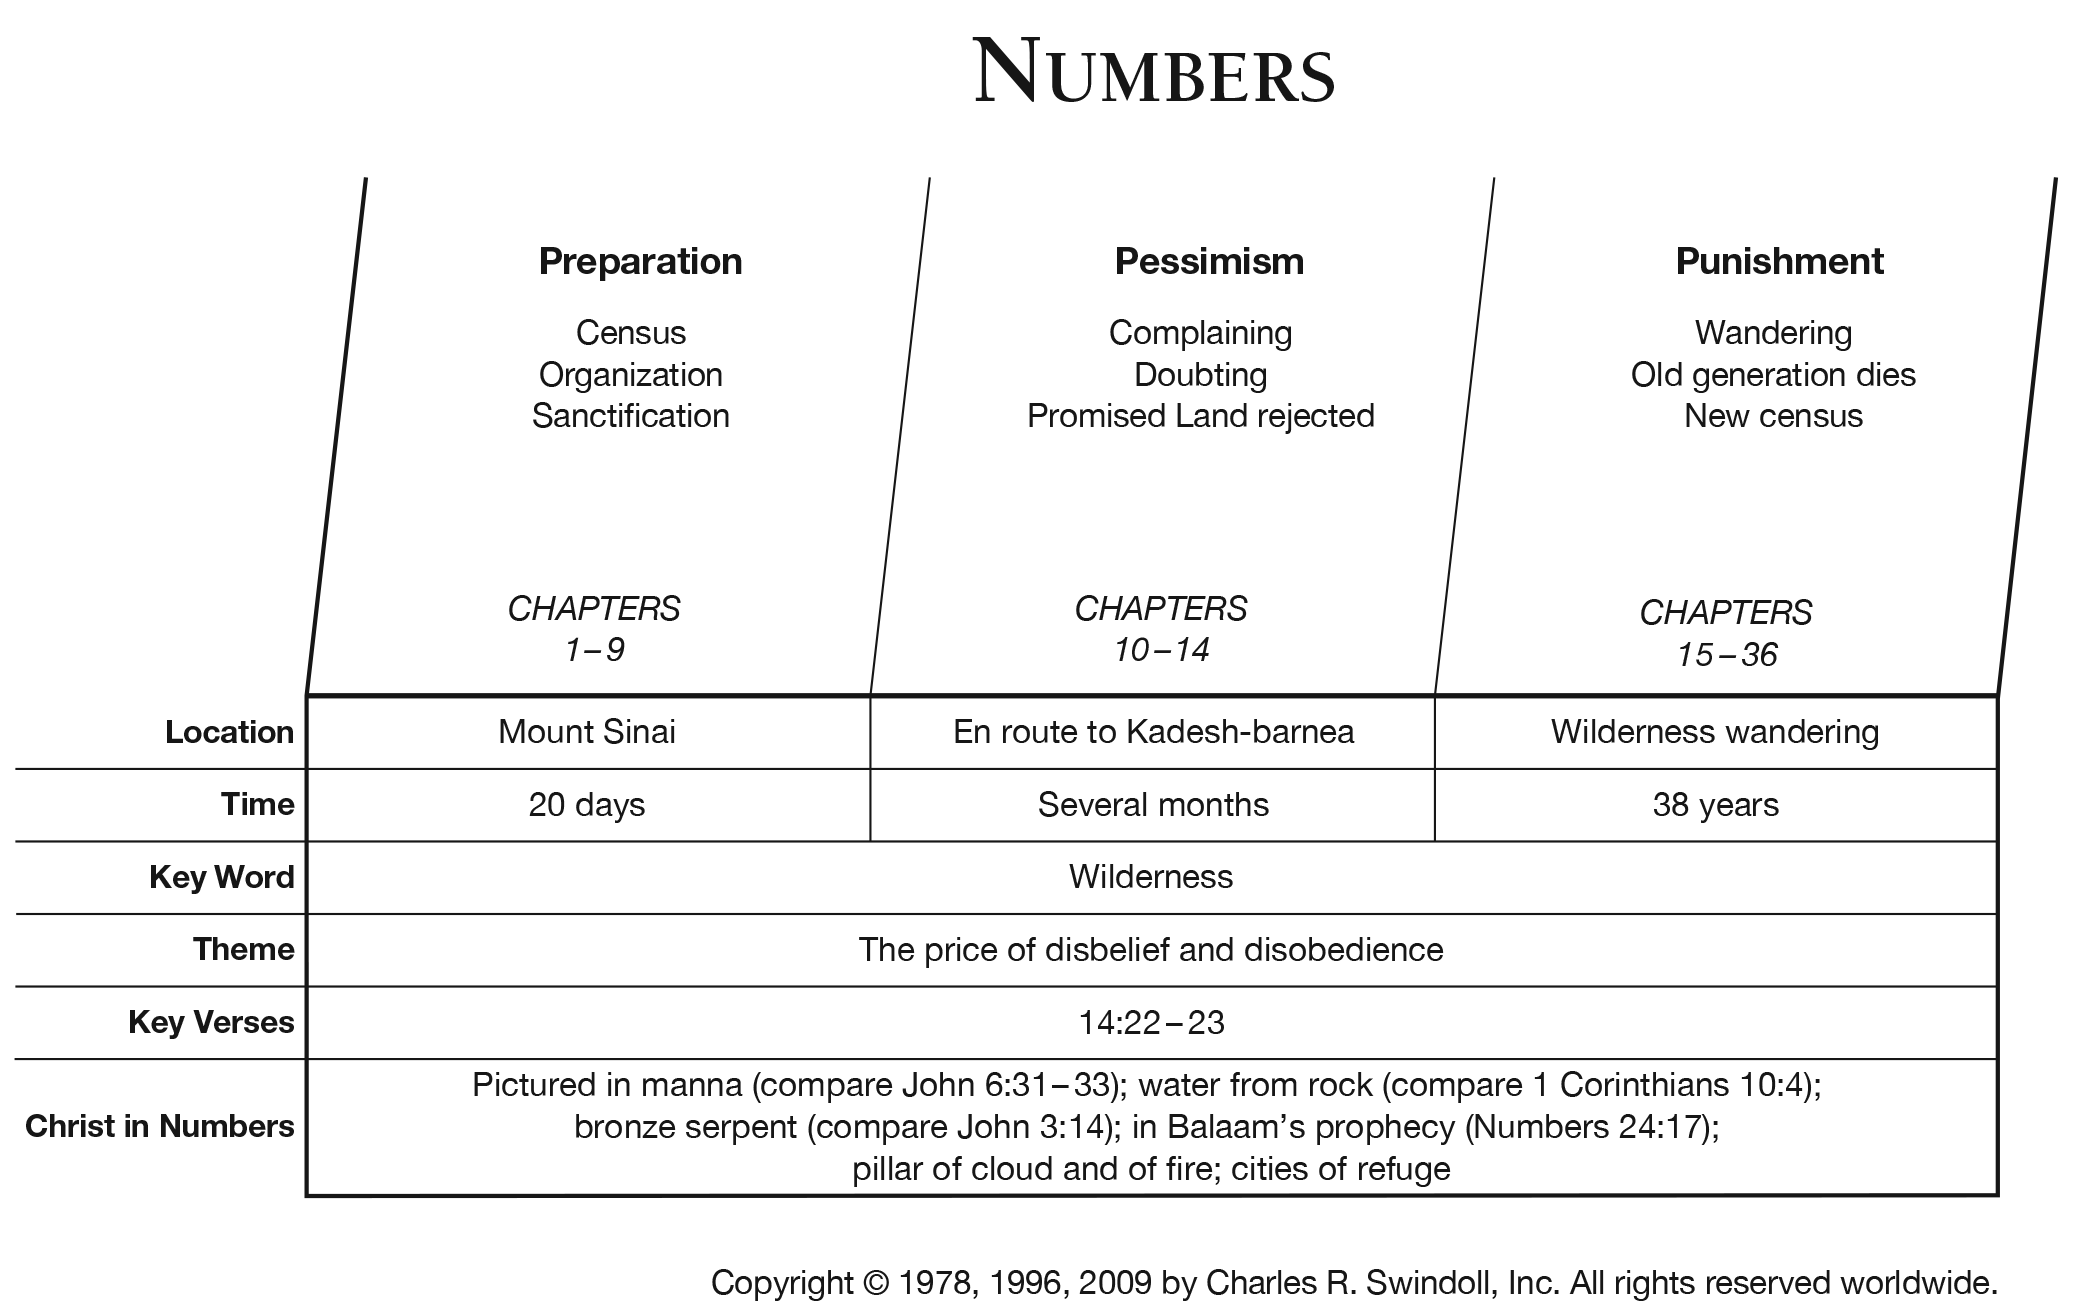
\includegraphics[scale=0.3, angle=90]{04OT-Numbers/References/Swindoll-Numbers.png}
\caption[Numbers by Swindoll]{Numbers by Swindoll}
\label{fig:Numbers by Swindoll}
\end{center}
\end{figure}

\newpage
\begin{figure}
\begin{center}
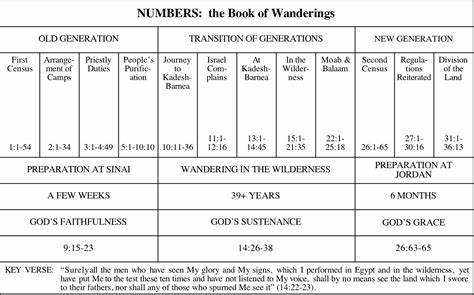
\includegraphics[scale=1.2, angle=90]{04OT-Numbers/References/Numbers.jpg}
\caption[Numbers by Unknown]{Numbers by Unknown}
\label{fig:Numbers by Unknown}
\end{center}
\end{figure}

\newpage
\begin{figure}
\begin{center}
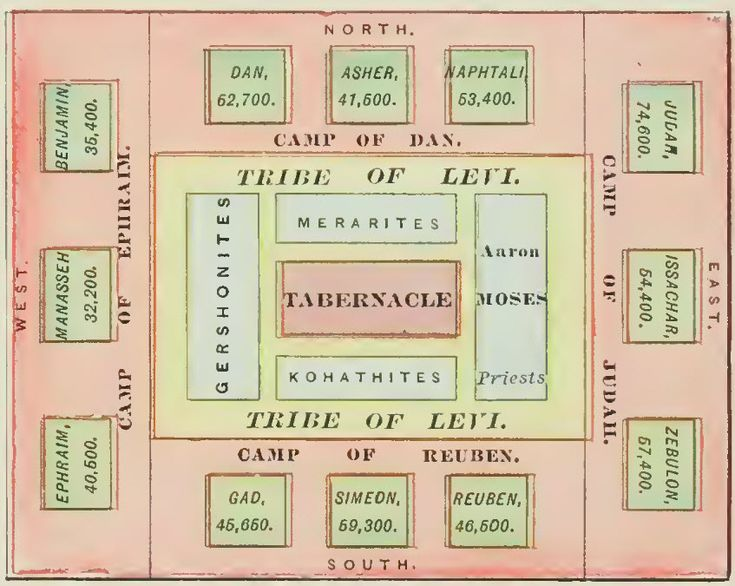
\includegraphics[scale=.8, angle=0]{04OT-Numbers/References/LayoutOfTribesAndTabernacle.jpg}
\caption[Layout of Tribes and Tabernacle]{Layout of Tribes and Tabernacle}
\label{fig:Layout of Tribes and Tabernacle}
\end{center}
\end{figure}


\chapter{Numbers 25}

\begin{figure}
  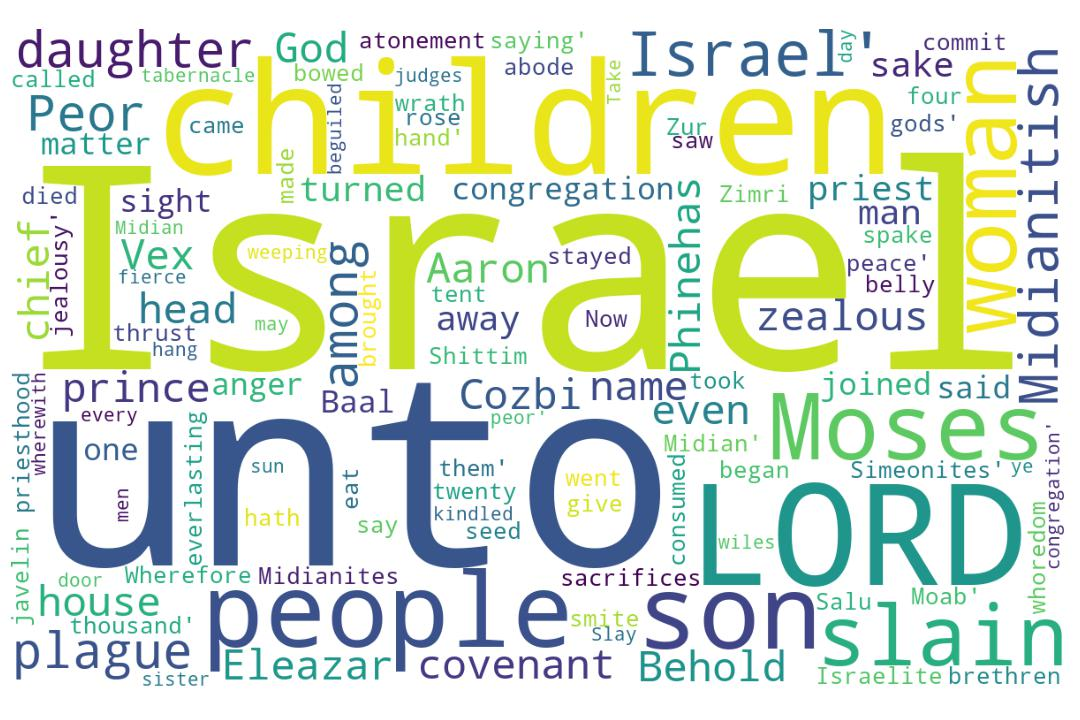
\includegraphics[width=\linewidth]{04OT-Numbers/Numbers25-WordCloud.jpg}
  \caption{Numbers 25 Word Cloud}
  \label{fig:Numbers 25 word Cloud}
\end{figure}

\marginpar{\scriptsize \centering \fcolorbox{bone}{lime}{\textbf{WORSHIP W THE MIDIANITES}}\\ (Numbers 25)
\begin{compactenum}[I.][8]
	\item Go to \textbf{Church} with us \index[scripture]{Numbers!Num 25:02} (Numbers 25:2)
    \item Get \textbf{Carnal} with us \index[scripture]{Numbers!Num 25:02} (Numbers 25:2)
    \item Get \textbf{Corrupted} with us \index[scripture]{Numbers!Num 25:02} (Numbers 25:2)
    \item Get \textbf{Condemned} with us \index[scripture]{Numbers!Num 25:02} (Numbers 25:2)
    \item Get \textbf{Corrected} without us \index[scripture]{Numbers!Num 25:04} (Numbers 25:4)
    \item Get \textbf{Cleansed} within us \index[scripture]{Numbers!Num 25:07} (Numbers 25:7)
\end{compactenum}}

\marginpar{\scriptsize \centering \fcolorbox{bone}{yellow}{\textbf{MAKING A POINT}}\\ (Numbers 25)
\begin{compactenum}[I.][8]
    \item The \textbf{Midianite Prince} with us \index[scripture]{Numbers!Num 25:15} (Numbers 25:15)
    \item The \textbf{Midianite Problem} \index[scripture]{Numbers!Num 25:13} (Numbers 25:13)
    \item A \textbf{Motivated Priest} \index[scripture]{Numbers!Num 25:06} (Numbers 25:6)
    \item A \textbf{Mighty Passion} \index[scripture]{Numbers!Num 25:13} (Numbers 25:13)
    \item A \textbf{Majestic Promise} \index[scripture]{Numbers!Num 25:13} (Numbers 25:13)
    \item This \textbf{Man Phineas} \index[scripture]{Numbers!Num 25:07} (Numbers 25:7)
\end{compactenum}}

%%%%%%%%%%%%%%%%%%%%%%%%%%%%%%%%%%
%%%%%%%%%%%%%%%%%%%%%%%%%%%%%%%%%%
\footnote{\textcolor[rgb]{0.00,0.25,0.00}{\hyperlink{TOC}{Return to end of Table of Contents.}}}\footnote{\href{https://audiobible.com/bible/numbers_25.html}{\textcolor[cmyk]{0.99998,1,0,0}{Numbers 25 Audio}}}\textcolor[cmyk]{0.99998,1,0,0}{\fcolorbox{bone}{bone}{And} \fcolorbox{bone}{bone}{Israel} abode in Shittim, and the people began to commit whoredom with the daughters of Moab.}
[2] \textcolor[cmyk]{0.99998,1,0,0}{\fcolorbox{bone}{bone}{And} they called the people unto the sacrifices of their gods: and the people did eat, and bowed down to their gods.}
[3] \textcolor[cmyk]{0.99998,1,0,0}{\fcolorbox{bone}{bone}{And} \fcolorbox{bone}{bone}{Israel} joined himself unto Baal-peor: and the anger of the LORD was kindled against \fcolorbox{bone}{bone}{Israel}.}
[4] \textcolor[cmyk]{0.99998,1,0,0}{\fcolorbox{bone}{bone}{And} the LORD said unto Moses, Take all the heads of the people, and hang them up before the LORD against the sun, that the fierce anger of the LORD may be turned away from \fcolorbox{bone}{bone}{Israel}.}
[5] \textcolor[cmyk]{0.99998,1,0,0}{\fcolorbox{bone}{bone}{And} Moses said unto the judges of \fcolorbox{bone}{bone}{Israel}, Slay ye every one his men that were joined unto Baal-peor.}\\
\\
\P \textcolor[cmyk]{0.99998,1,0,0}{\fcolorbox{bone}{bone}{And}, behold, one of the children of \fcolorbox{bone}{bone}{Israel} came and brought unto his brethren a Midianitish woman in the sight of Moses, and in the sight of all the congregation of the children of \fcolorbox{bone}{bone}{Israel}, who \emph{were} weeping \emph{before} the door of the tabernacle of the congregation.}
[7] \textcolor[cmyk]{0.99998,1,0,0}{\fcolorbox{bone}{bone}{And} when Phinehas, the son of Eleazar, the son of Aaron the priest, saw \emph{it}, he rose up from among the congregation, and took a javelin in his hand;}
[8] \textcolor[cmyk]{0.99998,1,0,0}{\fcolorbox{bone}{bone}{And} he went after the man of \fcolorbox{bone}{bone}{Israel} into the tent, and thrust both of them through, the man of \fcolorbox{bone}{bone}{Israel}, and the woman through her belly. So the plague was stayed from the children of \fcolorbox{bone}{bone}{Israel}.}
[9] \textcolor[cmyk]{0.99998,1,0,0}{\fcolorbox{bone}{bone}{And} those that died in the plague were twenty and four thousand.}\\
\\
\P  \textcolor[cmyk]{0.99998,1,0,0}{\fcolorbox{bone}{bone}{And} the LORD spake unto Moses, saying,}
[11] \textcolor[cmyk]{0.99998,1,0,0}{Phinehas, the son of Eleazar, the son of Aaron the priest, hath turned my wrath away from the children of \fcolorbox{bone}{bone}{Israel}, while he was zealous for my sake among them, that I consumed not the children of \fcolorbox{bone}{bone}{Israel} in my jealousy.}
[12] \textcolor[cmyk]{0.99998,1,0,0}{Wherefore say, Behold, I give unto him my covenant of peace:}
[13] \textcolor[cmyk]{0.99998,1,0,0}{\fcolorbox{bone}{bone}{And} he shall have it, and his seed after him, \emph{even} the covenant of an everlasting priesthood; because he was zealous for his God, and made an atonement for the children of \fcolorbox{bone}{bone}{Israel}.}
[14] \textcolor[cmyk]{0.99998,1,0,0}{Now the name of the Israelite that was slain, \emph{even} that was slain with the Midianitish woman, \emph{was} Zimri, the son of Salu, a prince of a chief house among the Simeonites.}
[15] \textcolor[cmyk]{0.99998,1,0,0}{\fcolorbox{bone}{bone}{And} the name of the Midianitish woman that was slain \emph{was} Cozbi, the daughter of Zur; he \emph{was} head over a people, \emph{and} of a chief house in Midian.}\\
\\
\P \textcolor[cmyk]{0.99998,1,0,0}{\fcolorbox{bone}{bone}{And} the LORD spake unto Moses, saying,}
[17] \textcolor[cmyk]{0.99998,1,0,0}{Vex the Midianites, and smite them:}
[18] \textcolor[cmyk]{0.99998,1,0,0}{For they vex you with their wiles, wherewith they have beguiled you in the matter of Peor, and in the matter of Cozbi, the daughter of a prince of Midian, their sister, which was slain in the day of the plague for Peor's sake.}
\index[NWIV]{17!Numbers!Num 25:1}\index[AWIP]{And!Numbers!Num 25:1}\index[AWIP]{Israel!Numbers!Num 25:1}\index[AWIP]{abode!Numbers!Num 25:1}\index[AWIP]{in!Numbers!Num 25:1}\index[AWIP]{Shittim!Numbers!Num 25:1}\index[AWIP]{and!Numbers!Num 25:1}\index[AWIP]{the!Numbers!Num 25:1}\index[AWIP]{the!Numbers!Num 25:1 (2)}\index[AWIP]{people!Numbers!Num 25:1}\index[AWIP]{began!Numbers!Num 25:1}\index[AWIP]{to!Numbers!Num 25:1}\index[AWIP]{commit!Numbers!Num 25:1}\index[AWIP]{whoredom!Numbers!Num 25:1}\index[AWIP]{with!Numbers!Num 25:1}\index[AWIP]{daughters!Numbers!Num 25:1}\index[AWIP]{of!Numbers!Num 25:1}\index[AWIP]{Moab!Numbers!Num 25:1}

\index[NWIV]{22!Numbers!Num 25:2}\index[AWIP]{And!Numbers!Num 25:2}\index[AWIP]{they!Numbers!Num 25:2}\index[AWIP]{called!Numbers!Num 25:2}\index[AWIP]{the!Numbers!Num 25:2}\index[AWIP]{the!Numbers!Num 25:2 (2)}\index[AWIP]{the!Numbers!Num 25:2 (3)}\index[AWIP]{people!Numbers!Num 25:2}\index[AWIP]{people!Numbers!Num 25:2 (2)}\index[AWIP]{unto!Numbers!Num 25:2}\index[AWIP]{sacrifices!Numbers!Num 25:2}\index[AWIP]{of!Numbers!Num 25:2}\index[AWIP]{their!Numbers!Num 25:2}\index[AWIP]{their!Numbers!Num 25:2 (2)}\index[AWIP]{gods!Numbers!Num 25:2}\index[AWIP]{gods!Numbers!Num 25:2 (2)}\index[AWIP]{and!Numbers!Num 25:2}\index[AWIP]{and!Numbers!Num 25:2 (2)}\index[AWIP]{did!Numbers!Num 25:2}\index[AWIP]{eat!Numbers!Num 25:2}\index[AWIP]{bowed!Numbers!Num 25:2}\index[AWIP]{down!Numbers!Num 25:2}\index[AWIP]{to!Numbers!Num 25:2}

\index[NWIV]{16!Numbers!Num 25:3}\index[AWIP]{And!Numbers!Num 25:3}\index[AWIP]{Israel!Numbers!Num 25:3}\index[AWIP]{Israel!Numbers!Num 25:3 (2)}\index[AWIP]{joined!Numbers!Num 25:3}\index[AWIP]{himself!Numbers!Num 25:3}\index[AWIP]{unto!Numbers!Num 25:3}\index[AWIP]{Baal-peor!Numbers!Num 25:3}\index[AWIP]{and!Numbers!Num 25:3}\index[AWIP]{the!Numbers!Num 25:3}\index[AWIP]{the!Numbers!Num 25:3 (2)}\index[AWIP]{anger!Numbers!Num 25:3}\index[AWIP]{of!Numbers!Num 25:3}\index[AWIP]{LORD!Numbers!Num 25:3}\index[AWIP]{was!Numbers!Num 25:3}\index[AWIP]{kindled!Numbers!Num 25:3}\index[AWIP]{against!Numbers!Num 25:3}

\index[NWIV]{36!Numbers!Num 25:4}\index[AWIP]{And!Numbers!Num 25:4}\index[AWIP]{the!Numbers!Num 25:4}\index[AWIP]{the!Numbers!Num 25:4 (2)}\index[AWIP]{the!Numbers!Num 25:4 (3)}\index[AWIP]{the!Numbers!Num 25:4 (4)}\index[AWIP]{the!Numbers!Num 25:4 (5)}\index[AWIP]{the!Numbers!Num 25:4 (6)}\index[AWIP]{the!Numbers!Num 25:4 (7)}\index[AWIP]{LORD!Numbers!Num 25:4}\index[AWIP]{LORD!Numbers!Num 25:4 (2)}\index[AWIP]{LORD!Numbers!Num 25:4 (3)}\index[AWIP]{said!Numbers!Num 25:4}\index[AWIP]{unto!Numbers!Num 25:4}\index[AWIP]{Moses!Numbers!Num 25:4}\index[AWIP]{Take!Numbers!Num 25:4}\index[AWIP]{all!Numbers!Num 25:4}\index[AWIP]{heads!Numbers!Num 25:4}\index[AWIP]{of!Numbers!Num 25:4}\index[AWIP]{of!Numbers!Num 25:4 (2)}\index[AWIP]{people!Numbers!Num 25:4}\index[AWIP]{and!Numbers!Num 25:4}\index[AWIP]{hang!Numbers!Num 25:4}\index[AWIP]{them!Numbers!Num 25:4}\index[AWIP]{up!Numbers!Num 25:4}\index[AWIP]{before!Numbers!Num 25:4}\index[AWIP]{against!Numbers!Num 25:4}\index[AWIP]{sun!Numbers!Num 25:4}\index[AWIP]{that!Numbers!Num 25:4}\index[AWIP]{fierce!Numbers!Num 25:4}\index[AWIP]{anger!Numbers!Num 25:4}\index[AWIP]{may!Numbers!Num 25:4}\index[AWIP]{be!Numbers!Num 25:4}\index[AWIP]{turned!Numbers!Num 25:4}\index[AWIP]{away!Numbers!Num 25:4}\index[AWIP]{from!Numbers!Num 25:4}\index[AWIP]{Israel!Numbers!Num 25:4}

\index[NWIV]{19!Numbers!Num 25:5}\index[AWIP]{And!Numbers!Num 25:5}\index[AWIP]{Moses!Numbers!Num 25:5}\index[AWIP]{said!Numbers!Num 25:5}\index[AWIP]{unto!Numbers!Num 25:5}\index[AWIP]{unto!Numbers!Num 25:5 (2)}\index[AWIP]{the!Numbers!Num 25:5}\index[AWIP]{judges!Numbers!Num 25:5}\index[AWIP]{of!Numbers!Num 25:5}\index[AWIP]{Israel!Numbers!Num 25:5}\index[AWIP]{Slay!Numbers!Num 25:5}\index[AWIP]{ye!Numbers!Num 25:5}\index[AWIP]{every!Numbers!Num 25:5}\index[AWIP]{one!Numbers!Num 25:5}\index[AWIP]{his!Numbers!Num 25:5}\index[AWIP]{men!Numbers!Num 25:5}\index[AWIP]{that!Numbers!Num 25:5}\index[AWIP]{were!Numbers!Num 25:5}\index[AWIP]{joined!Numbers!Num 25:5}\index[AWIP]{Baal-peor!Numbers!Num 25:5}

\index[NWIV]{47!Numbers!Num 25:6}\index[AWIP]{And!Numbers!Num 25:6}\index[AWIP]{behold!Numbers!Num 25:6}\index[AWIP]{one!Numbers!Num 25:6}\index[AWIP]{of!Numbers!Num 25:6}\index[AWIP]{of!Numbers!Num 25:6 (2)}\index[AWIP]{of!Numbers!Num 25:6 (3)}\index[AWIP]{of!Numbers!Num 25:6 (4)}\index[AWIP]{of!Numbers!Num 25:6 (5)}\index[AWIP]{of!Numbers!Num 25:6 (6)}\index[AWIP]{of!Numbers!Num 25:6 (7)}\index[AWIP]{of!Numbers!Num 25:6 (8)}\index[AWIP]{the!Numbers!Num 25:6}\index[AWIP]{the!Numbers!Num 25:6 (2)}\index[AWIP]{the!Numbers!Num 25:6 (3)}\index[AWIP]{the!Numbers!Num 25:6 (4)}\index[AWIP]{the!Numbers!Num 25:6 (5)}\index[AWIP]{the!Numbers!Num 25:6 (6)}\index[AWIP]{the!Numbers!Num 25:6 (7)}\index[AWIP]{the!Numbers!Num 25:6 (8)}\index[AWIP]{children!Numbers!Num 25:6}\index[AWIP]{children!Numbers!Num 25:6 (2)}\index[AWIP]{Israel!Numbers!Num 25:6}\index[AWIP]{Israel!Numbers!Num 25:6 (2)}\index[AWIP]{came!Numbers!Num 25:6}\index[AWIP]{and!Numbers!Num 25:6}\index[AWIP]{and!Numbers!Num 25:6 (2)}\index[AWIP]{brought!Numbers!Num 25:6}\index[AWIP]{unto!Numbers!Num 25:6}\index[AWIP]{his!Numbers!Num 25:6}\index[AWIP]{brethren!Numbers!Num 25:6}\index[AWIP]{a!Numbers!Num 25:6}\index[AWIP]{Midianitish!Numbers!Num 25:6}\index[AWIP]{woman!Numbers!Num 25:6}\index[AWIP]{in!Numbers!Num 25:6}\index[AWIP]{in!Numbers!Num 25:6 (2)}\index[AWIP]{sight!Numbers!Num 25:6}\index[AWIP]{sight!Numbers!Num 25:6 (2)}\index[AWIP]{Moses!Numbers!Num 25:6}\index[AWIP]{all!Numbers!Num 25:6}\index[AWIP]{congregation!Numbers!Num 25:6}\index[AWIP]{congregation!Numbers!Num 25:6 (2)}\index[AWIP]{who!Numbers!Num 25:6}\index[AWIP]{\emph{were}!Numbers!Num 25:6}\index[AWIP]{weeping!Numbers!Num 25:6}\index[AWIP]{\emph{before}!Numbers!Num 25:6}\index[AWIP]{door!Numbers!Num 25:6}\index[AWIP]{tabernacle!Numbers!Num 25:6}\index[AWIP]{\emph{were}!Numbers!Num 25:6}\index[AWIP]{\emph{before}!Numbers!Num 25:6}

\index[NWIV]{29!Numbers!Num 25:7}\index[AWIP]{And!Numbers!Num 25:7}\index[AWIP]{when!Numbers!Num 25:7}\index[AWIP]{Phinehas!Numbers!Num 25:7}\index[AWIP]{the!Numbers!Num 25:7}\index[AWIP]{the!Numbers!Num 25:7 (2)}\index[AWIP]{the!Numbers!Num 25:7 (3)}\index[AWIP]{the!Numbers!Num 25:7 (4)}\index[AWIP]{son!Numbers!Num 25:7}\index[AWIP]{son!Numbers!Num 25:7 (2)}\index[AWIP]{of!Numbers!Num 25:7}\index[AWIP]{of!Numbers!Num 25:7 (2)}\index[AWIP]{Eleazar!Numbers!Num 25:7}\index[AWIP]{Aaron!Numbers!Num 25:7}\index[AWIP]{priest!Numbers!Num 25:7}\index[AWIP]{saw!Numbers!Num 25:7}\index[AWIP]{\emph{it}!Numbers!Num 25:7}\index[AWIP]{he!Numbers!Num 25:7}\index[AWIP]{rose!Numbers!Num 25:7}\index[AWIP]{up!Numbers!Num 25:7}\index[AWIP]{from!Numbers!Num 25:7}\index[AWIP]{among!Numbers!Num 25:7}\index[AWIP]{congregation!Numbers!Num 25:7}\index[AWIP]{and!Numbers!Num 25:7}\index[AWIP]{took!Numbers!Num 25:7}\index[AWIP]{a!Numbers!Num 25:7}\index[AWIP]{javelin!Numbers!Num 25:7}\index[AWIP]{in!Numbers!Num 25:7}\index[AWIP]{his!Numbers!Num 25:7}\index[AWIP]{hand!Numbers!Num 25:7}\index[AWIP]{\emph{it}!Numbers!Num 25:7}

\index[NWIV]{37!Numbers!Num 25:8}\index[AWIP]{And!Numbers!Num 25:8}\index[AWIP]{he!Numbers!Num 25:8}\index[AWIP]{went!Numbers!Num 25:8}\index[AWIP]{after!Numbers!Num 25:8}\index[AWIP]{the!Numbers!Num 25:8}\index[AWIP]{the!Numbers!Num 25:8 (2)}\index[AWIP]{the!Numbers!Num 25:8 (3)}\index[AWIP]{the!Numbers!Num 25:8 (4)}\index[AWIP]{the!Numbers!Num 25:8 (5)}\index[AWIP]{the!Numbers!Num 25:8 (6)}\index[AWIP]{man!Numbers!Num 25:8}\index[AWIP]{man!Numbers!Num 25:8 (2)}\index[AWIP]{of!Numbers!Num 25:8}\index[AWIP]{of!Numbers!Num 25:8 (2)}\index[AWIP]{of!Numbers!Num 25:8 (3)}\index[AWIP]{of!Numbers!Num 25:8 (4)}\index[AWIP]{Israel!Numbers!Num 25:8}\index[AWIP]{Israel!Numbers!Num 25:8 (2)}\index[AWIP]{Israel!Numbers!Num 25:8 (3)}\index[AWIP]{into!Numbers!Num 25:8}\index[AWIP]{tent!Numbers!Num 25:8}\index[AWIP]{and!Numbers!Num 25:8}\index[AWIP]{and!Numbers!Num 25:8 (2)}\index[AWIP]{thrust!Numbers!Num 25:8}\index[AWIP]{both!Numbers!Num 25:8}\index[AWIP]{them!Numbers!Num 25:8}\index[AWIP]{through!Numbers!Num 25:8}\index[AWIP]{through!Numbers!Num 25:8 (2)}\index[AWIP]{woman!Numbers!Num 25:8}\index[AWIP]{her!Numbers!Num 25:8}\index[AWIP]{belly!Numbers!Num 25:8}\index[AWIP]{So!Numbers!Num 25:8}\index[AWIP]{plague!Numbers!Num 25:8}\index[AWIP]{was!Numbers!Num 25:8}\index[AWIP]{stayed!Numbers!Num 25:8}\index[AWIP]{from!Numbers!Num 25:8}\index[AWIP]{children!Numbers!Num 25:8}

\index[NWIV]{12!Numbers!Num 25:9}\index[AWIP]{And!Numbers!Num 25:9}\index[AWIP]{those!Numbers!Num 25:9}\index[AWIP]{that!Numbers!Num 25:9}\index[AWIP]{died!Numbers!Num 25:9}\index[AWIP]{in!Numbers!Num 25:9}\index[AWIP]{the!Numbers!Num 25:9}\index[AWIP]{plague!Numbers!Num 25:9}\index[AWIP]{were!Numbers!Num 25:9}\index[AWIP]{twenty!Numbers!Num 25:9}\index[AWIP]{and!Numbers!Num 25:9}\index[AWIP]{four!Numbers!Num 25:9}\index[AWIP]{thousand!Numbers!Num 25:9}

\index[NWIV]{7!Numbers!Num 25:10}\index[AWIP]{And!Numbers!Num 25:10}\index[AWIP]{the!Numbers!Num 25:10}\index[AWIP]{LORD!Numbers!Num 25:10}\index[AWIP]{spake!Numbers!Num 25:10}\index[AWIP]{unto!Numbers!Num 25:10}\index[AWIP]{Moses!Numbers!Num 25:10}\index[AWIP]{saying!Numbers!Num 25:10}

\index[NWIV]{41!Numbers!Num 25:11}\index[AWIP]{Phinehas!Numbers!Num 25:11}\index[AWIP]{the!Numbers!Num 25:11}\index[AWIP]{the!Numbers!Num 25:11 (2)}\index[AWIP]{the!Numbers!Num 25:11 (3)}\index[AWIP]{the!Numbers!Num 25:11 (4)}\index[AWIP]{the!Numbers!Num 25:11 (5)}\index[AWIP]{son!Numbers!Num 25:11}\index[AWIP]{son!Numbers!Num 25:11 (2)}\index[AWIP]{of!Numbers!Num 25:11}\index[AWIP]{of!Numbers!Num 25:11 (2)}\index[AWIP]{of!Numbers!Num 25:11 (3)}\index[AWIP]{of!Numbers!Num 25:11 (4)}\index[AWIP]{Eleazar!Numbers!Num 25:11}\index[AWIP]{Aaron!Numbers!Num 25:11}\index[AWIP]{priest!Numbers!Num 25:11}\index[AWIP]{hath!Numbers!Num 25:11}\index[AWIP]{turned!Numbers!Num 25:11}\index[AWIP]{my!Numbers!Num 25:11}\index[AWIP]{my!Numbers!Num 25:11 (2)}\index[AWIP]{my!Numbers!Num 25:11 (3)}\index[AWIP]{wrath!Numbers!Num 25:11}\index[AWIP]{away!Numbers!Num 25:11}\index[AWIP]{from!Numbers!Num 25:11}\index[AWIP]{children!Numbers!Num 25:11}\index[AWIP]{children!Numbers!Num 25:11 (2)}\index[AWIP]{Israel!Numbers!Num 25:11}\index[AWIP]{Israel!Numbers!Num 25:11 (2)}\index[AWIP]{while!Numbers!Num 25:11}\index[AWIP]{he!Numbers!Num 25:11}\index[AWIP]{was!Numbers!Num 25:11}\index[AWIP]{zealous!Numbers!Num 25:11}\index[AWIP]{for!Numbers!Num 25:11}\index[AWIP]{sake!Numbers!Num 25:11}\index[AWIP]{among!Numbers!Num 25:11}\index[AWIP]{them!Numbers!Num 25:11}\index[AWIP]{that!Numbers!Num 25:11}\index[AWIP]{I!Numbers!Num 25:11}\index[AWIP]{consumed!Numbers!Num 25:11}\index[AWIP]{not!Numbers!Num 25:11}\index[AWIP]{in!Numbers!Num 25:11}\index[AWIP]{jealousy!Numbers!Num 25:11}

\index[NWIV]{11!Numbers!Num 25:12}\index[AWIP]{Wherefore!Numbers!Num 25:12}\index[AWIP]{say!Numbers!Num 25:12}\index[AWIP]{Behold!Numbers!Num 25:12}\index[AWIP]{I!Numbers!Num 25:12}\index[AWIP]{give!Numbers!Num 25:12}\index[AWIP]{unto!Numbers!Num 25:12}\index[AWIP]{him!Numbers!Num 25:12}\index[AWIP]{my!Numbers!Num 25:12}\index[AWIP]{covenant!Numbers!Num 25:12}\index[AWIP]{of!Numbers!Num 25:12}\index[AWIP]{peace!Numbers!Num 25:12}

\index[NWIV]{33!Numbers!Num 25:13}\index[AWIP]{And!Numbers!Num 25:13}\index[AWIP]{he!Numbers!Num 25:13}\index[AWIP]{he!Numbers!Num 25:13 (2)}\index[AWIP]{shall!Numbers!Num 25:13}\index[AWIP]{have!Numbers!Num 25:13}\index[AWIP]{it!Numbers!Num 25:13}\index[AWIP]{and!Numbers!Num 25:13}\index[AWIP]{and!Numbers!Num 25:13 (2)}\index[AWIP]{his!Numbers!Num 25:13}\index[AWIP]{his!Numbers!Num 25:13 (2)}\index[AWIP]{seed!Numbers!Num 25:13}\index[AWIP]{after!Numbers!Num 25:13}\index[AWIP]{him!Numbers!Num 25:13}\index[AWIP]{\emph{even}!Numbers!Num 25:13}\index[AWIP]{the!Numbers!Num 25:13}\index[AWIP]{the!Numbers!Num 25:13 (2)}\index[AWIP]{covenant!Numbers!Num 25:13}\index[AWIP]{of!Numbers!Num 25:13}\index[AWIP]{of!Numbers!Num 25:13 (2)}\index[AWIP]{an!Numbers!Num 25:13}\index[AWIP]{an!Numbers!Num 25:13 (2)}\index[AWIP]{everlasting!Numbers!Num 25:13}\index[AWIP]{priesthood!Numbers!Num 25:13}\index[AWIP]{because!Numbers!Num 25:13}\index[AWIP]{was!Numbers!Num 25:13}\index[AWIP]{zealous!Numbers!Num 25:13}\index[AWIP]{for!Numbers!Num 25:13}\index[AWIP]{for!Numbers!Num 25:13 (2)}\index[AWIP]{God!Numbers!Num 25:13}\index[AWIP]{made!Numbers!Num 25:13}\index[AWIP]{atonement!Numbers!Num 25:13}\index[AWIP]{children!Numbers!Num 25:13}\index[AWIP]{Israel!Numbers!Num 25:13}\index[AWIP]{\emph{even}!Numbers!Num 25:13}

\index[NWIV]{32!Numbers!Num 25:14}\index[AWIP]{Now!Numbers!Num 25:14}\index[AWIP]{the!Numbers!Num 25:14}\index[AWIP]{the!Numbers!Num 25:14 (2)}\index[AWIP]{the!Numbers!Num 25:14 (3)}\index[AWIP]{the!Numbers!Num 25:14 (4)}\index[AWIP]{the!Numbers!Num 25:14 (5)}\index[AWIP]{name!Numbers!Num 25:14}\index[AWIP]{of!Numbers!Num 25:14}\index[AWIP]{of!Numbers!Num 25:14 (2)}\index[AWIP]{of!Numbers!Num 25:14 (3)}\index[AWIP]{Israelite!Numbers!Num 25:14}\index[AWIP]{that!Numbers!Num 25:14}\index[AWIP]{that!Numbers!Num 25:14 (2)}\index[AWIP]{was!Numbers!Num 25:14}\index[AWIP]{was!Numbers!Num 25:14 (2)}\index[AWIP]{slain!Numbers!Num 25:14}\index[AWIP]{slain!Numbers!Num 25:14 (2)}\index[AWIP]{\emph{even}!Numbers!Num 25:14}\index[AWIP]{with!Numbers!Num 25:14}\index[AWIP]{Midianitish!Numbers!Num 25:14}\index[AWIP]{woman!Numbers!Num 25:14}\index[AWIP]{\emph{was}!Numbers!Num 25:14}\index[AWIP]{Zimri!Numbers!Num 25:14}\index[AWIP]{son!Numbers!Num 25:14}\index[AWIP]{Salu!Numbers!Num 25:14}\index[AWIP]{a!Numbers!Num 25:14}\index[AWIP]{a!Numbers!Num 25:14 (2)}\index[AWIP]{prince!Numbers!Num 25:14}\index[AWIP]{chief!Numbers!Num 25:14}\index[AWIP]{house!Numbers!Num 25:14}\index[AWIP]{among!Numbers!Num 25:14}\index[AWIP]{Simeonites!Numbers!Num 25:14}\index[AWIP]{\emph{even}!Numbers!Num 25:14}\index[AWIP]{\emph{was}!Numbers!Num 25:14}

\index[NWIV]{29!Numbers!Num 25:15}\index[AWIP]{And!Numbers!Num 25:15}\index[AWIP]{the!Numbers!Num 25:15}\index[AWIP]{the!Numbers!Num 25:15 (2)}\index[AWIP]{the!Numbers!Num 25:15 (3)}\index[AWIP]{name!Numbers!Num 25:15}\index[AWIP]{of!Numbers!Num 25:15}\index[AWIP]{of!Numbers!Num 25:15 (2)}\index[AWIP]{of!Numbers!Num 25:15 (3)}\index[AWIP]{Midianitish!Numbers!Num 25:15}\index[AWIP]{woman!Numbers!Num 25:15}\index[AWIP]{that!Numbers!Num 25:15}\index[AWIP]{was!Numbers!Num 25:15}\index[AWIP]{slain!Numbers!Num 25:15}\index[AWIP]{\emph{was}!Numbers!Num 25:15}\index[AWIP]{\emph{was}!Numbers!Num 25:15 (2)}\index[AWIP]{Cozbi!Numbers!Num 25:15}\index[AWIP]{daughter!Numbers!Num 25:15}\index[AWIP]{Zur!Numbers!Num 25:15}\index[AWIP]{he!Numbers!Num 25:15}\index[AWIP]{head!Numbers!Num 25:15}\index[AWIP]{over!Numbers!Num 25:15}\index[AWIP]{a!Numbers!Num 25:15}\index[AWIP]{a!Numbers!Num 25:15 (2)}\index[AWIP]{people!Numbers!Num 25:15}\index[AWIP]{\emph{and}!Numbers!Num 25:15}\index[AWIP]{chief!Numbers!Num 25:15}\index[AWIP]{house!Numbers!Num 25:15}\index[AWIP]{in!Numbers!Num 25:15}\index[AWIP]{Midian!Numbers!Num 25:15}\index[AWIP]{\emph{was}!Numbers!Num 25:15}\index[AWIP]{\emph{was}!Numbers!Num 25:15 (2)}\index[AWIP]{\emph{and}!Numbers!Num 25:15}

\index[NWIV]{7!Numbers!Num 25:16}\index[AWIP]{And!Numbers!Num 25:16}\index[AWIP]{the!Numbers!Num 25:16}\index[AWIP]{LORD!Numbers!Num 25:16}\index[AWIP]{spake!Numbers!Num 25:16}\index[AWIP]{unto!Numbers!Num 25:16}\index[AWIP]{Moses!Numbers!Num 25:16}\index[AWIP]{saying!Numbers!Num 25:16}

\index[NWIV]{6!Numbers!Num 25:17}\index[AWIP]{Vex!Numbers!Num 25:17}\index[AWIP]{the!Numbers!Num 25:17}\index[AWIP]{Midianites!Numbers!Num 25:17}\index[AWIP]{and!Numbers!Num 25:17}\index[AWIP]{smite!Numbers!Num 25:17}\index[AWIP]{them!Numbers!Num 25:17}

\index[NWIV]{44!Numbers!Num 25:18}\index[AWIP]{For!Numbers!Num 25:18}\index[AWIP]{they!Numbers!Num 25:18}\index[AWIP]{they!Numbers!Num 25:18 (2)}\index[AWIP]{vex!Numbers!Num 25:18}\index[AWIP]{you!Numbers!Num 25:18}\index[AWIP]{you!Numbers!Num 25:18 (2)}\index[AWIP]{with!Numbers!Num 25:18}\index[AWIP]{their!Numbers!Num 25:18}\index[AWIP]{their!Numbers!Num 25:18 (2)}\index[AWIP]{wiles!Numbers!Num 25:18}\index[AWIP]{wherewith!Numbers!Num 25:18}\index[AWIP]{have!Numbers!Num 25:18}\index[AWIP]{beguiled!Numbers!Num 25:18}\index[AWIP]{in!Numbers!Num 25:18}\index[AWIP]{in!Numbers!Num 25:18 (2)}\index[AWIP]{in!Numbers!Num 25:18 (3)}\index[AWIP]{the!Numbers!Num 25:18}\index[AWIP]{the!Numbers!Num 25:18 (2)}\index[AWIP]{the!Numbers!Num 25:18 (3)}\index[AWIP]{the!Numbers!Num 25:18 (4)}\index[AWIP]{the!Numbers!Num 25:18 (5)}\index[AWIP]{matter!Numbers!Num 25:18}\index[AWIP]{matter!Numbers!Num 25:18 (2)}\index[AWIP]{of!Numbers!Num 25:18}\index[AWIP]{of!Numbers!Num 25:18 (2)}\index[AWIP]{of!Numbers!Num 25:18 (3)}\index[AWIP]{of!Numbers!Num 25:18 (4)}\index[AWIP]{of!Numbers!Num 25:18 (5)}\index[AWIP]{Peor!Numbers!Num 25:18}\index[AWIP]{and!Numbers!Num 25:18}\index[AWIP]{Cozbi!Numbers!Num 25:18}\index[AWIP]{daughter!Numbers!Num 25:18}\index[AWIP]{a!Numbers!Num 25:18}\index[AWIP]{prince!Numbers!Num 25:18}\index[AWIP]{Midian!Numbers!Num 25:18}\index[AWIP]{sister!Numbers!Num 25:18}\index[AWIP]{which!Numbers!Num 25:18}\index[AWIP]{was!Numbers!Num 25:18}\index[AWIP]{slain!Numbers!Num 25:18}\index[AWIP]{day!Numbers!Num 25:18}\index[AWIP]{plague!Numbers!Num 25:18}\index[AWIP]{for!Numbers!Num 25:18}\index[AWIP]{Peor's!Numbers!Num 25:18}\index[AWIP]{sake!Numbers!Num 25:18}


\section{Numbers 25 Outlines}

\subsection{My Outlines}

\subsubsection{Worshiping with the Midianites}
\index[speaker]{Keith Anthony!Numbers 25 (Worshiping with the Midianites)}
\index[series]{Numbers (Keith Anthony)!Numbers 25 (Worshiping with the Midianites)}
\index[date]{2017/02/18!Numbers 25 (Worshiping with the Midianites) (Keith Anthony)}
Numbers 25 details the implementation of the doctrine of Balaam, how God felt about it, and what the results were:
\begin{compactenum}[I.]
    \item Go to \textbf{Church} with us \index[scripture]{Numbers!Num 25:02} (Numbers 25:2)
    \item Get \textbf{Carnal} with us \index[scripture]{Numbers!Num 25:02} (Numbers 25:2)
    \item Get \textbf{Corrupted} with us \index[scripture]{Numbers!Num 25:02} (Numbers 25:2)
    \item Get \textbf{Condemned} with us \index[scripture]{Numbers!Num 25:02} (Numbers 25:2)
    \item Get \textbf{Corrected} without us \index[scripture]{Numbers!Num 25:04} (Numbers 25:4)
    \item Get \textbf{Cleansed} within us \index[scripture]{Numbers!Num 25:07} (Numbers 25:7)
\end{compactenum}

\subsubsection{Making a Point}
\index[speaker]{Keith Anthony!Numbers 25 (Making a Point)}
\index[series]{Numbers (Keith Anthony)!Numbers 25 (Making a Point)}
\index[date]{2018/02/19!Numbers 25 (Making a Point (Keith Anthony)}
\begin{compactenum}[I.][7]
    \item The \textbf{Midianite Prince} with us \index[scripture]{Numbers!Num 25:15} (Numbers 25:15)
    \item The \textbf{Midianite Problem} \index[scripture]{Numbers!Num 25:13} (Numbers 25:13)
    \item A \textbf{Motivated Priest} \index[scripture]{Numbers!Num 25:06} (Numbers 25:6)
    \item A \textbf{Mighty Passion} \index[scripture]{Numbers!Num 25:13} (Numbers 25:13)
    \item A \textbf{Majestic Promise} \index[scripture]{Numbers!Num 25:13} (Numbers 25:13)
    \item This \textbf{Man Phineas} \index[scripture]{Numbers!Num 25:07} (Numbers 25:7)
\end{compactenum}

%%% wiles, woman, woes, watchers, wrath
%%%  beguiling, bringing, bothering, blessing
\subsection{Outlines from Others}
\section{Numbers 25 Comments}

\subsection{Numeric Nuggets}
\textbf{13: } The words ``Israel'' and ``And'' are used 13 times in the chapter.


\subsection{Numbers 25 Repeated Phrases}


%%%%%%%%%%
%%%%%%%%%%
\normalsize
 
\begin{center}
\begin{longtable}{|p{3.0in}|p{0.5in}|}
\caption[Numbers 25 Repeated Phrases]{Numbers 25 Repeated Phrases}\label{table:Repeated Phrases Numbers 25} \\
\hline \multicolumn{1}{|c|}{\textbf{Phrase}} & \multicolumn{1}{c|}{\textbf{Frequency}} \\ \hline 
\endfirsthead
 
\multicolumn{2}{c}
{{\bfseries \tablename\ \thetable{} -- continued from previous page}} \\  
\hline \multicolumn{1}{|c|}{\textbf{Phrase}} & \multicolumn{1}{c|}{\textbf{Frequency}} \\ \hline 
\endhead
 
\hline \multicolumn{2}{c}{{ }} \\ \hline
\endfoot 
of the & 10\\ \hline 
of Israel & 9\\ \hline 
the LORD & 6\\ \hline 
the children & 6\\ \hline 
the children of & 6\\ \hline 
the children of Israel & 6\\ \hline 
children of & 6\\ \hline 
children of Israel & 6\\ \hline 
in the & 6\\ \hline 
the son & 5\\ \hline 
the son of & 5\\ \hline 
son of & 5\\ \hline 
and the & 4\\ \hline 
the people & 4\\ \hline 
And the & 4\\ \hline 
was slain & 4\\ \hline 
And the LORD & 3\\ \hline 
unto Moses & 3\\ \hline 
Midianitish woman & 3\\ \hline 
the congregation & 3\\ \hline 
the plague & 3\\ \hline 
that was & 3\\ \hline 
that was slain & 3\\ \hline 
of a & 3\\ \hline 
\end{longtable}
\end{center}



%%%%%%%%%%
%%%%%%%%%%



\section{Numbers 25 Word Statistics}


%%%%%%%%%%
%%%%%%%%%%
\normalsize
 
\begin{center}
\begin{longtable}{l|c|c|c|c}
\caption[Numbers 25 Statistics]{Numbers 25 Statistics}\label{table:Statistics for Numbers 25} \\
\hline \multicolumn{1}{|c|}{\textbf{Verse(s)}} & \multicolumn{1}{|c|}{\textbf{Count}} & \multicolumn{1}{|c|}{\textbf{Unique}} & \multicolumn{1}{|c|}{\textbf{Italics}} & \multicolumn{1}{|c|}{\textbf{Uniq Italic}}  \\ \hline 
\endfirsthead
 
\multicolumn{5}{c}
{{\bfseries \tablename\ \thetable{} -- continued from previous page}} \\  
\hline \multicolumn{1}{|c|}{\textbf{Verse(s)}} & \multicolumn{1}{|c|}{\textbf{Count}} & \multicolumn{1}{|c|}{\textbf{Unique}} & \multicolumn{1}{|c|}{\textbf{Italics}} & \multicolumn{1}{|c|}{\textbf{Uniq Italic}}  \\ \hline 
\endhead
 
\hline \multicolumn{5}{|r|}{{Continued if needed}} \\ \hline
\endfoot 
1 & 17 & 16 & 0 & 0\\ \hline
2 & 22 & 16 & 0 & 0\\ \hline
3 & 16 & 14 & 0 & 0\\ \hline
4 & 36 & 27 & 0 & 0\\ \hline
5 & 19 & 18 & 0 & 0\\ \hline
6 & 47 & 27 & 2 & 2\\ \hline
7 & 29 & 24 & 1 & 1\\ \hline
8 & 37 & 24 & 0 & 0\\ \hline
9 & 12 & 12 & 0 & 0\\ \hline
10 & 7 & 7 & 0 & 0\\ \hline
11 & 41 & 29 & 0 & 0\\ \hline
12 & 11 & 11 & 0 & 0\\ \hline
13 & 33 & 26 & 1 & 1\\ \hline
14 & 32 & 22 & 2 & 2\\ \hline
15 & 29 & 23 & 3 & 2\\ \hline
16 & 7 & 7 & 0 & 0\\ \hline
17 & 6 & 6 & 0 & 0\\ \hline
18 & 44 & 30 & 0 & 0\\ \hline
Total & 445 & 172 & 9 & 6
\end{longtable}
\end{center}



%%%%%%%%%%
%%%%%%%%%%


\subsection{Numbers 25 Words by Frequency}


%%%%%%%%%%
%%%%%%%%%%
\normalsize
 
\begin{center}
\begin{longtable}{l|r}
\caption[Numbers 25 Words by Frequency]{Numbers 25 Words by Frequency}\label{table:WordsbyFrequency for Numbers 25} \\
\hline \multicolumn{1}{|c|}{\textbf{Word}} & \multicolumn{1}{c|}{\textbf{Frequency}} \\ \hline 
\endfirsthead
 
\multicolumn{2}{c}
{{\bfseries \tablename\ \thetable{} -- continued from previous page}} \\  
\hline \multicolumn{1}{|c|}{\textbf{Word}} & \multicolumn{1}{c|}{\textbf{Frequency}} \\ \hline 
\endhead
 
\hline \multicolumn{2}{c}{{ }} \\ \hline
\endfoot 
the & 57\\ \hline 
of & 38\\ \hline 
and & 15\\ \hline 
And & 13\\ \hline 
Israel & 13\\ \hline 
in & 10\\ \hline 
unto & 9\\ \hline 
was & 8\\ \hline 
that & 7\\ \hline 
a & 7\\ \hline 
LORD & 6\\ \hline 
children & 6\\ \hline 
he & 6\\ \hline 
people & 5\\ \hline 
Moses & 5\\ \hline 
his & 5\\ \hline 
son & 5\\ \hline 
their & 4\\ \hline 
them & 4\\ \hline 
from & 4\\ \hline 
woman & 4\\ \hline 
my & 4\\ \hline 
for & 4\\ \hline 
slain & 4\\ \hline 
with & 3\\ \hline 
they & 3\\ \hline 
Midianitish & 3\\ \hline 
congregation & 3\\ \hline 
among & 3\\ \hline 
plague & 3\\ \hline 
\emph{was} & 3\\ \hline 
to & 2\\ \hline 
gods & 2\\ \hline 
joined & 2\\ \hline 
Baal-peor & 2\\ \hline 
anger & 2\\ \hline 
against & 2\\ \hline 
said & 2\\ \hline 
all & 2\\ \hline 
up & 2\\ \hline 
turned & 2\\ \hline 
away & 2\\ \hline 
one & 2\\ \hline 
were & 2\\ \hline 
sight & 2\\ \hline 
Phinehas & 2\\ \hline 
Eleazar & 2\\ \hline 
Aaron & 2\\ \hline 
priest & 2\\ \hline 
after & 2\\ \hline 
man & 2\\ \hline 
through & 2\\ \hline 
spake & 2\\ \hline 
saying & 2\\ \hline 
zealous & 2\\ \hline 
sake & 2\\ \hline 
I & 2\\ \hline 
him & 2\\ \hline 
covenant & 2\\ \hline 
have & 2\\ \hline 
\emph{even} & 2\\ \hline 
an & 2\\ \hline 
name & 2\\ \hline 
prince & 2\\ \hline 
chief & 2\\ \hline 
house & 2\\ \hline 
Cozbi & 2\\ \hline 
daughter & 2\\ \hline 
Midian & 2\\ \hline 
you & 2\\ \hline 
matter & 2\\ \hline 
abode & 1\\ \hline 
Shittim & 1\\ \hline 
began & 1\\ \hline 
commit & 1\\ \hline 
whoredom & 1\\ \hline 
daughters & 1\\ \hline 
Moab & 1\\ \hline 
called & 1\\ \hline 
sacrifices & 1\\ \hline 
did & 1\\ \hline 
eat & 1\\ \hline 
bowed & 1\\ \hline 
down & 1\\ \hline 
himself & 1\\ \hline 
kindled & 1\\ \hline 
Take & 1\\ \hline 
heads & 1\\ \hline 
hang & 1\\ \hline 
before & 1\\ \hline 
sun & 1\\ \hline 
fierce & 1\\ \hline 
may & 1\\ \hline 
be & 1\\ \hline 
judges & 1\\ \hline 
Slay & 1\\ \hline 
ye & 1\\ \hline 
every & 1\\ \hline 
men & 1\\ \hline 
behold & 1\\ \hline 
came & 1\\ \hline 
brought & 1\\ \hline 
brethren & 1\\ \hline 
who & 1\\ \hline 
\emph{were} & 1\\ \hline 
weeping & 1\\ \hline 
\emph{before} & 1\\ \hline 
door & 1\\ \hline 
tabernacle & 1\\ \hline 
when & 1\\ \hline 
saw & 1\\ \hline 
\emph{it} & 1\\ \hline 
rose & 1\\ \hline 
took & 1\\ \hline 
javelin & 1\\ \hline 
hand & 1\\ \hline 
went & 1\\ \hline 
into & 1\\ \hline 
tent & 1\\ \hline 
thrust & 1\\ \hline 
both & 1\\ \hline 
her & 1\\ \hline 
belly & 1\\ \hline 
So & 1\\ \hline 
stayed & 1\\ \hline 
those & 1\\ \hline 
died & 1\\ \hline 
twenty & 1\\ \hline 
four & 1\\ \hline 
thousand & 1\\ \hline 
hath & 1\\ \hline 
wrath & 1\\ \hline 
while & 1\\ \hline 
consumed & 1\\ \hline 
not & 1\\ \hline 
jealousy & 1\\ \hline 
Wherefore & 1\\ \hline 
say & 1\\ \hline 
Behold & 1\\ \hline 
give & 1\\ \hline 
peace & 1\\ \hline 
shall & 1\\ \hline 
it & 1\\ \hline 
seed & 1\\ \hline 
everlasting & 1\\ \hline 
priesthood & 1\\ \hline 
because & 1\\ \hline 
God & 1\\ \hline 
made & 1\\ \hline 
atonement & 1\\ \hline 
Now & 1\\ \hline 
Israelite & 1\\ \hline 
Zimri & 1\\ \hline 
Salu & 1\\ \hline 
Simeonites & 1\\ \hline 
Zur & 1\\ \hline 
head & 1\\ \hline 
over & 1\\ \hline 
\emph{and} & 1\\ \hline 
Vex & 1\\ \hline 
Midianites & 1\\ \hline 
smite & 1\\ \hline 
For & 1\\ \hline 
vex & 1\\ \hline 
wiles & 1\\ \hline 
wherewith & 1\\ \hline 
beguiled & 1\\ \hline 
Peor & 1\\ \hline 
sister & 1\\ \hline 
which & 1\\ \hline 
day & 1\\ \hline 
Peor's & 1\\ \hline 
\end{longtable}
\end{center}



%%%%%%%%%%
%%%%%%%%%%


\subsection{Numbers 25 Words Alphabetically}


%%%%%%%%%%
%%%%%%%%%%
\normalsize
 
\begin{center}
\begin{longtable}{l|r}
\caption[Numbers 25 Words Alphabetically]{Numbers 25 Words Alphabetically}\label{table:WordsAlphabetically for Numbers 25} \\
\hline \multicolumn{1}{|c|}{\textbf{Word}} & \multicolumn{1}{c|}{\textbf{Frequency}} \\ \hline 
\endfirsthead
 
\multicolumn{2}{c}
{{\bfseries \tablename\ \thetable{} -- continued from previous page}} \\  
\hline \multicolumn{1}{|c|}{\textbf{Word}} & \multicolumn{1}{c|}{\textbf{Frequency}} \\ \hline 
\endhead
 
\hline \multicolumn{2}{c}{{ }} \\ \hline
\endfoot 
Aaron & 2\\ \hline 
And & 13\\ \hline 
Baal-peor & 2\\ \hline 
Behold & 1\\ \hline 
Cozbi & 2\\ \hline 
Eleazar & 2\\ \hline 
For & 1\\ \hline 
God & 1\\ \hline 
I & 2\\ \hline 
Israel & 13\\ \hline 
Israelite & 1\\ \hline 
LORD & 6\\ \hline 
Midian & 2\\ \hline 
Midianites & 1\\ \hline 
Midianitish & 3\\ \hline 
Moab & 1\\ \hline 
Moses & 5\\ \hline 
Now & 1\\ \hline 
Peor & 1\\ \hline 
Peor's & 1\\ \hline 
Phinehas & 2\\ \hline 
Salu & 1\\ \hline 
Shittim & 1\\ \hline 
Simeonites & 1\\ \hline 
Slay & 1\\ \hline 
So & 1\\ \hline 
Take & 1\\ \hline 
Vex & 1\\ \hline 
Wherefore & 1\\ \hline 
Zimri & 1\\ \hline 
Zur & 1\\ \hline 
\emph{and} & 1\\ \hline 
\emph{before} & 1\\ \hline 
\emph{even} & 2\\ \hline 
\emph{it} & 1\\ \hline 
\emph{was} & 3\\ \hline 
\emph{were} & 1\\ \hline 
a & 7\\ \hline 
abode & 1\\ \hline 
after & 2\\ \hline 
against & 2\\ \hline 
all & 2\\ \hline 
among & 3\\ \hline 
an & 2\\ \hline 
and & 15\\ \hline 
anger & 2\\ \hline 
atonement & 1\\ \hline 
away & 2\\ \hline 
be & 1\\ \hline 
because & 1\\ \hline 
before & 1\\ \hline 
began & 1\\ \hline 
beguiled & 1\\ \hline 
behold & 1\\ \hline 
belly & 1\\ \hline 
both & 1\\ \hline 
bowed & 1\\ \hline 
brethren & 1\\ \hline 
brought & 1\\ \hline 
called & 1\\ \hline 
came & 1\\ \hline 
chief & 2\\ \hline 
children & 6\\ \hline 
commit & 1\\ \hline 
congregation & 3\\ \hline 
consumed & 1\\ \hline 
covenant & 2\\ \hline 
daughter & 2\\ \hline 
daughters & 1\\ \hline 
day & 1\\ \hline 
did & 1\\ \hline 
died & 1\\ \hline 
door & 1\\ \hline 
down & 1\\ \hline 
eat & 1\\ \hline 
everlasting & 1\\ \hline 
every & 1\\ \hline 
fierce & 1\\ \hline 
for & 4\\ \hline 
four & 1\\ \hline 
from & 4\\ \hline 
give & 1\\ \hline 
gods & 2\\ \hline 
hand & 1\\ \hline 
hang & 1\\ \hline 
hath & 1\\ \hline 
have & 2\\ \hline 
he & 6\\ \hline 
head & 1\\ \hline 
heads & 1\\ \hline 
her & 1\\ \hline 
him & 2\\ \hline 
himself & 1\\ \hline 
his & 5\\ \hline 
house & 2\\ \hline 
in & 10\\ \hline 
into & 1\\ \hline 
it & 1\\ \hline 
javelin & 1\\ \hline 
jealousy & 1\\ \hline 
joined & 2\\ \hline 
judges & 1\\ \hline 
kindled & 1\\ \hline 
made & 1\\ \hline 
man & 2\\ \hline 
matter & 2\\ \hline 
may & 1\\ \hline 
men & 1\\ \hline 
my & 4\\ \hline 
name & 2\\ \hline 
not & 1\\ \hline 
of & 38\\ \hline 
one & 2\\ \hline 
over & 1\\ \hline 
peace & 1\\ \hline 
people & 5\\ \hline 
plague & 3\\ \hline 
priest & 2\\ \hline 
priesthood & 1\\ \hline 
prince & 2\\ \hline 
rose & 1\\ \hline 
sacrifices & 1\\ \hline 
said & 2\\ \hline 
sake & 2\\ \hline 
saw & 1\\ \hline 
say & 1\\ \hline 
saying & 2\\ \hline 
seed & 1\\ \hline 
shall & 1\\ \hline 
sight & 2\\ \hline 
sister & 1\\ \hline 
slain & 4\\ \hline 
smite & 1\\ \hline 
son & 5\\ \hline 
spake & 2\\ \hline 
stayed & 1\\ \hline 
sun & 1\\ \hline 
tabernacle & 1\\ \hline 
tent & 1\\ \hline 
that & 7\\ \hline 
the & 57\\ \hline 
their & 4\\ \hline 
them & 4\\ \hline 
they & 3\\ \hline 
those & 1\\ \hline 
thousand & 1\\ \hline 
through & 2\\ \hline 
thrust & 1\\ \hline 
to & 2\\ \hline 
took & 1\\ \hline 
turned & 2\\ \hline 
twenty & 1\\ \hline 
unto & 9\\ \hline 
up & 2\\ \hline 
vex & 1\\ \hline 
was & 8\\ \hline 
weeping & 1\\ \hline 
went & 1\\ \hline 
were & 2\\ \hline 
when & 1\\ \hline 
wherewith & 1\\ \hline 
which & 1\\ \hline 
while & 1\\ \hline 
who & 1\\ \hline 
whoredom & 1\\ \hline 
wiles & 1\\ \hline 
with & 3\\ \hline 
woman & 4\\ \hline 
wrath & 1\\ \hline 
ye & 1\\ \hline 
you & 2\\ \hline 
zealous & 2\\ \hline 
\end{longtable}
\end{center}



%%%%%%%%%%
%%%%%%%%%%


\subsection{Numbers 25 Words by Length}


%%%%%%%%%%
%%%%%%%%%%
\normalsize
 
\begin{center}
\begin{longtable}{l|p{3.75in}}
\caption[Numbers 25 Words by Length]{Numbers 25 Words by Length}\label{table:WordsAlphabetically for Numbers 25} \\
\hline \multicolumn{1}{|c|}{\textbf{Length}} & \multicolumn{1}{c|}{\textbf{Words}} \\ \hline 
\endfirsthead
\hline \multicolumn{1}{|c|}{\textbf{Length}} & \multicolumn{1}{c|}{\textbf{Words}} \\ \hline 
\multicolumn{2}{c}
{{\bfseries \tablename\ \thetable{} -- continued from previous page}} \\  
\hline \multicolumn{1}{|c|}{\textbf{Word}} & \multicolumn{1}{c|}{\textbf{Frequency}} \\ \hline 
\endhead
 
\hline \multicolumn{2}{c}{{ }} \\ \hline
\endfoot 
1 & a, I\\ \hline 
2 & in, to, of, up, be, ye, \emph{it}, he, So, my, it, an\\ \hline 
3 & And, and, the, did, eat, was, all, sun, may, one, his, men, who, son, saw, man, her, for, not, say, him, God, Now, \emph{was}, Zur, \emph{and}, Vex, For, vex, you, day\\ \hline 
4 & with, Moab, they, unto, gods, down, LORD, said, Take, hang, them, that, away, from, Slay, were, came, \emph{were}, door, when, rose, took, hand, went, into, tent, both, died, four, hath, sake, give, have, seed, \emph{even}, made, name, Salu, head, over, Peor\\ \hline 
5 & abode, began, their, bowed, anger, Moses, heads, every, woman, sight, Aaron, among, after, belly, those, spake, wrath, while, peace, shall, slain, Zimri, chief, house, Cozbi, smite, wiles, which\\ \hline 
6 & Israel, people, commit, called, joined, before, fierce, turned, judges, behold, \emph{before}, priest, thrust, plague, stayed, twenty, saying, Behold, prince, Midian, matter, sister, Peor's\\ \hline 
7 & Shittim, himself, kindled, against, brought, weeping, Eleazar, javelin, through, zealous, because\\ \hline 
8 & whoredom, children, brethren, Phinehas, thousand, consumed, jealousy, covenant, daughter, beguiled\\ \hline 
9 & daughters, Baal-peor, Wherefore, atonement, Israelite, wherewith\\ \hline 
10 & sacrifices, tabernacle, priesthood, Simeonites, Midianites\\ \hline 
11 & Midianitish, everlasting\\ \hline 
12 & congregation\\ \hline 
\end{longtable}
\end{center}



%%%%%%%%%%
%%%%%%%%%%




\chapter{Numbers 26}

\begin{figure}
  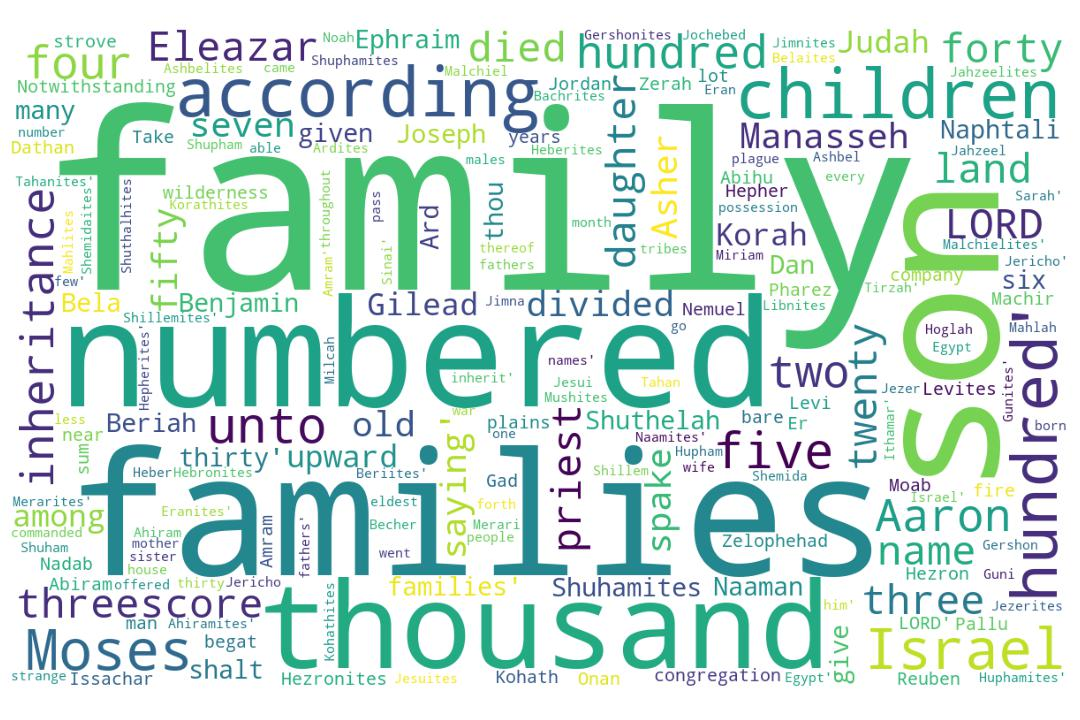
\includegraphics[width=\linewidth]{04OT-Numbers/Numbers26-WordCloud.jpg}
  \caption{Numbers 26 Word Cloud}
  \label{fig:Numbers 26 word Cloud}
\end{figure}

\marginpar{\scriptsize \centering \fcolorbox{bone}{lime}{\textbf{A GENERATION LATER}}\\ (Numbers 26)
\begin{compactenum}[I.][8]
    \item The \textbf{Priests} \index[scripture]{Numbers!Num 26:01}\index[scripture]{Numbers!Num 26:03}\index[scripture]{Numbers!Num 26:63}\index[scripture]{Numbers!Num 26:64} (Numbers 26:1, 3, 63, 64)
    \item The \textbf{Plague} \index[scripture]{Numbers!Num 26:01} (Numbers 26:1)
    \item The \textbf{Plains} of Moab \index[scripture]{Numbers!Num 26:03}\index[scripture]{Numbers!Num 26:64} (Numbers 26:3, 64)
    \item The \textbf{People} 
    \item The \textbf{Population} \index[scripture]{Numbers!Num 26:12--54} (Numbers 26:12--54) Note the differences in population among the various tribes. Simeon loses almost 63\% of its people, while some of the tribes grow substantially.
    \item The \textbf{Possessions} \index[scripture]{Numbers!Num 26:56} (Numbers 26:56)
    \item A \textbf{Preview} 
\end{compactenum}}

%%%%%%%%%%%%%%%%%%%%%%%%%%%%%%%%%%
%%%%%%%%%%%%%%%%%%%%%%%%%%%%%%%%%%
\footnote{\textcolor[rgb]{0.00,0.25,0.00}{\hyperlink{TOC}{Return to end of Table of Contents.}}}\footnote{\href{https://audiobible.com/bible/numbers_26.html}{\textcolor[cmyk]{0.99998,1,0,0}{Numbers 26 Audio}}}\textcolor[cmyk]{0.99998,1,0,0}{And it came to pass after the plague, that the LORD spake unto Moses and unto Eleazar the son of Aaron the priest, saying,}
[2] \textcolor[cmyk]{0.99998,1,0,0}{Take the sum of all the congregation of the children of Israel, from twenty years old and upward, throughout their fathers' house, all that are able to go to war in Israel.}
[3] \textcolor[cmyk]{0.99998,1,0,0}{And Moses and Eleazar the priest spake with them in the plains of Moab by Jordan \emph{near} Jericho, saying,}
[4] \textcolor[cmyk]{0.99998,1,0,0}{\emph{Take} \emph{the} \emph{sum} \emph{of} \emph{the} \emph{people}, from twenty years old and upward; as the LORD commanded Moses and the children of Israel, which went forth out of the land of Egypt.}\\
\\
\P \textcolor[cmyk]{0.99998,1,0,0}{Reuben, the eldest son of Israel: the children of Reuben; Hanoch, \emph{of} \emph{whom} \emph{cometh} the family of the Hanochites: of Pallu, the family of the Palluites:}
[6] \textcolor[cmyk]{0.99998,1,0,0}{Of Hezron, the family of the Hezronites: of Carmi, the family of the Carmites.}
[7] \textcolor[cmyk]{0.99998,1,0,0}{These \emph{are} \fcolorbox{bone}{bone}{the familes} of the Reubenites: and they that were numbered of them were forty and three \fcolorbox{bone}{bone}{thousand and} seven hundred and thirty.}
[8] \textcolor[cmyk]{0.99998,1,0,0}{And the sons of Pallu; Eliab.}
[9] \textcolor[cmyk]{0.99998,1,0,0}{And the sons of Eliab; Nemuel, and Dathan, and Abiram. This \emph{is} \emph{that} Dathan and Abiram, \emph{which} \emph{were} famous in the congregation, who strove against Moses and against Aaron in the company of Korah, when they strove against the LORD:}\footnote{\textbf{Numbers 16:1-3} - Now Korah, the son of Izhar, the son of Kohath, the son of Levi, and Dathan and Abiram, the sons of Eliab, and On, the son of Peleth, sons of Reuben, took men: [2] And they rose up before Moses, with certain of the children of Israel, two hundred and fifty princes of the assembly, famous in the congregation, men of renown: [3] And they gathered themselves together against Moses and against Aaron, and said unto them, Ye take too much upon you, seeing all the congregation are holy, every one of them, and the LORD is among them: wherefore then lift ye up yourselves above the congregation of the LORD?}\footnote{\textbf{Deuteronomy 11:6} - And what he did unto Dathan and Abiram, the sons of Eliab, the son of Reuben: how the earth opened her mouth, and swallowed them up, and their households, and their tents, and all the substance that was in their possession, in the midst of all Israel:}\footnote{\textbf{Psalm 106:17} - The earth opened and swallowed up Dathan, and covered the company of Abiram.}
[10] \textcolor[cmyk]{0.99998,1,0,0}{And the earth opened her mouth, and swallowed them up together with Korah, when that company died, what time the fire devoured two hundred and fifty men: and they became a sign.}
[11] \textcolor[cmyk]{0.99998,1,0,0}{Notwithstanding the children of Korah died not.}\\
\\
\P \textcolor[cmyk]{0.99998,1,0,0}{The sons of Simeon after their families: of Nemuel, the family of the Nemuelites: of Jamin, the family of the Jaminites: of Jachin, the family of the Jachinites:}
[13] \textcolor[cmyk]{0.99998,1,0,0}{Of Zerah, the family of the Zarhites: of Shaul, the family of the Shaulites.}
[14] \textcolor[cmyk]{0.99998,1,0,0}{These \emph{are} \fcolorbox{bone}{bone}{the familes} of the Simeonites, twenty and two \fcolorbox{bone}{bone}{thousand and} two hundred.}\\
\\
\P \textcolor[cmyk]{0.99998,1,0,0}{The children of Gad after their families: of Zephon, the family of the Zephonites: of Haggi, the family of the Haggites: of Shuni, the family of the Shunites:}
[16] \textcolor[cmyk]{0.99998,1,0,0}{Of Ozni, the family of the Oznites: of Eri, the family of the Erites:}
[17] \textcolor[cmyk]{0.99998,1,0,0}{Of Arod, the family of the Arodites: of Areli, the family of the Arelites.}
[18] \textcolor[cmyk]{0.99998,1,0,0}{These \emph{are} \fcolorbox{bone}{bone}{the familes} of the children of Gad according to those that were numbered of them, forty \fcolorbox{bone}{bone}{thousand and} five hundred.}\\
\\
\P \textcolor[cmyk]{0.99998,1,0,0}{The sons of Judah \emph{were} Er and Onan: and Er and Onan died in the land of Canaan.}
[20] \textcolor[cmyk]{0.99998,1,0,0}{And the sons of Judah after their families were; of Shelah, the family of the Shelanites: of Pharez, the family of the Pharzites: of Zerah, the family of the Zarhites.}
[21] \textcolor[cmyk]{0.99998,1,0,0}{And the sons of Pharez were; of Hezron, the family of the Hezronites: of Hamul, the family of the Hamulites.}
[22] \textcolor[cmyk]{0.99998,1,0,0}{These \emph{are} \fcolorbox{bone}{bone}{the familes} of Judah according to those that were numbered of them, threescore and sixteen \fcolorbox{bone}{bone}{thousand and} five hundred.}\\
\\
\P \textcolor[cmyk]{0.99998,1,0,0}{\emph{Of} the sons of Issachar after their families: \emph{of} Tola, the family of the Tolaites: of Pua, the family of the Punites:}
[24] \textcolor[cmyk]{0.99998,1,0,0}{Of Jashub, the family of the Jashubites: of Shimron, the family of the Shimronites.}
[25] \textcolor[cmyk]{0.99998,1,0,0}{These \emph{are} \fcolorbox{bone}{bone}{the familes} of Issachar according to those that were numbered of them, threescore and four \fcolorbox{bone}{bone}{thousand and} three hundred.}\\
\\
\P \textcolor[cmyk]{0.99998,1,0,0}{\emph{Of} the sons of Zebulun after their families: of Sered, the family of the Sardites: of Elon, the family of the Elonites: of Jahleel, the family of the Jahleelites.}
[27] \textcolor[cmyk]{0.99998,1,0,0}{These \emph{are} \fcolorbox{bone}{bone}{the familes} of the Zebulunites according to those that were numbered of them, threescore \fcolorbox{bone}{bone}{thousand and} five hundred.}\\
\\
\P \textcolor[cmyk]{0.99998,1,0,0}{The sons of Joseph after their families \emph{were} Manasseh and Ephraim.}
[29] \textcolor[cmyk]{0.99998,1,0,0}{Of the sons of Manasseh: of Machir, the family of the Machirites: and Machir begat Gilead: of Gilead \emph{come} the family of the Gileadites.}
[30] \textcolor[cmyk]{0.99998,1,0,0}{These \emph{are} the sons of Gilead: \emph{of} Jeezer, the family of the Jeezerites: of Helek, the family of the Helekites:}
[31] \textcolor[cmyk]{0.99998,1,0,0}{And \emph{of} Asriel, the family of the Asrielites: and \emph{of} Shechem, the family of the Shechemites:}
[32] \textcolor[cmyk]{0.99998,1,0,0}{And \emph{of} Shemida, the family of the Shemidaites: and \emph{of} Hepher, the family of the Hepherites.}
[33] \textcolor[cmyk]{0.99998,1,0,0}{And Zelophehad the son of Hepher had no sons, but daughters: and the names of the daughters of Zelophehad \emph{were} Mahlah, and Noah, Hoglah, Milcah, and Tirzah.}
[34] \textcolor[cmyk]{0.99998,1,0,0}{These \emph{are} \fcolorbox{bone}{bone}{the familes} of Manasseh, and those that were numbered of them, fifty and two \fcolorbox{bone}{bone}{thousand and} seven hundred.}\\
\\
\P \textcolor[cmyk]{0.99998,1,0,0}{These \emph{are} the sons of Ephraim after their families: of Shuthelah, the family of the Shuthalhites: of Becher, the family of the Bachrites: of Tahan, the family of the Tahanites.}
[36] \textcolor[cmyk]{0.99998,1,0,0}{And these \emph{are} the sons of Shuthelah: of Eran, the family of the Eranites.}
[37] \textcolor[cmyk]{0.99998,1,0,0}{These \emph{are} \fcolorbox{bone}{bone}{the familes} of the sons of Ephraim according to those that were numbered of them, thirty and two \fcolorbox{bone}{bone}{thousand and} five hundred. These \emph{are} the sons of Joseph after their families.}\\
\\
\P \textcolor[cmyk]{0.99998,1,0,0}{The sons of Benjamin after their families: of Bela, the family of the Belaites: of Ashbel, the family of the Ashbelites: of Ahiram, the family of the Ahiramites:}
[39] \textcolor[cmyk]{0.99998,1,0,0}{Of Shupham, the family of the Shuphamites: of Hupham, the family of the Huphamites.}
[40] \textcolor[cmyk]{0.99998,1,0,0}{And the sons of Bela were Ard and Naaman: \emph{of} \emph{Ard}, the family of the Ardites: \emph{and} of Naaman, the family of the Naamites.}
[41] \textcolor[cmyk]{0.99998,1,0,0}{These \emph{are} the sons of Benjamin after their families: and they that were numbered of them \emph{were} forty and five \fcolorbox{bone}{bone}{thousand and} six hundred.}\\
\\
\P \textcolor[cmyk]{0.99998,1,0,0}{These \emph{are} the sons of Dan after their families: of Shuham, the family of the Shuhamites. These \emph{are} \fcolorbox{bone}{bone}{the familes} of Dan after their families.}
[43] \textcolor[cmyk]{0.99998,1,0,0}{All \fcolorbox{bone}{bone}{the familes} of the Shuhamites, according to those that were numbered of them, \emph{were} threescore and four \fcolorbox{bone}{bone}{thousand and} four hundred.}\\
\\
\P \textcolor[cmyk]{0.99998,1,0,0}{\emph{Of} the children of Asher after their families: of Jimna, the family of the Jimnites: of Jesui, the family of the Jesuites: of Beriah, the family of the Beriites.}
[45] \textcolor[cmyk]{0.99998,1,0,0}{Of the sons of Beriah: of Heber, the family of the Heberites: of Malchiel, the family of the Malchielites.}
[46] \textcolor[cmyk]{0.99998,1,0,0}{And the name of the daughter of Asher \emph{was} Sarah.}
[47] \textcolor[cmyk]{0.99998,1,0,0}{These \emph{are} \fcolorbox{bone}{bone}{the familes} of the sons of Asher according to those that were numbered of them; \emph{who} \emph{were} fifty and three \fcolorbox{bone}{bone}{thousand and} four hundred.}\\
\\
\P \textcolor[cmyk]{0.99998,1,0,0}{\emph{Of} the sons of Naphtali after their families: of Jahzeel, the family of the Jahzeelites: of Guni, the family of the Gunites:}
[49] \textcolor[cmyk]{0.99998,1,0,0}{Of Jezer, the family of the Jezerites: of Shillem, the family of the Shillemites.}
[50] \textcolor[cmyk]{0.99998,1,0,0}{These \emph{are} \fcolorbox{bone}{bone}{the familes} of Naphtali according to their families: and they that were numbered of them \emph{were} forty and five \fcolorbox{bone}{bone}{thousand and} four hundred.}
[51] \textcolor[cmyk]{0.99998,1,0,0}{These \emph{were} the numbered of the children of Israel, six hundred \fcolorbox{bone}{bone}{thousand and} a thousand seven hundred and thirty.}\\
\\
\P \textcolor[cmyk]{0.99998,1,0,0}{And the LORD spake unto Moses, saying,}
[53] \textcolor[cmyk]{0.99998,1,0,0}{Unto these the land shall be divided for an inheritance according to the number of names.}
[54] \textcolor[cmyk]{0.99998,1,0,0}{To many thou shalt give the more inheritance, and to few thou shalt give the less inheritance: to every one shall his inheritance be given according to those that were numbered of him.}
[55] \textcolor[cmyk]{0.99998,1,0,0}{Notwithstanding the land shall be divided by lot: according to the names of the tribes of their fathers they shall inherit.}
[56] \textcolor[cmyk]{0.99998,1,0,0}{According to the lot shall the possession thereof be divided between many and few.}\\
\\
\P \textcolor[cmyk]{0.99998,1,0,0}{And these \emph{are} they that were numbered of the Levites after their families: of Gershon, the family of the Gershonites: of Kohath, the family of the Kohathites: of Merari, the family of the Merarites.}
[58] \textcolor[cmyk]{0.99998,1,0,0}{These \emph{are} \fcolorbox{bone}{bone}{the familes} of the Levites: the family of the Libnites, the family of the Hebronites, the family of the Mahlites, the family of the Mushites, the family of the Korathites. And Kohath begat Amram.}
[59] \textcolor[cmyk]{0.99998,1,0,0}{And the name of Amram's wife \emph{was} Jochebed, the daughter of Levi, whom \emph{her} \emph{mother} bare to Levi in Egypt: and she bare unto Amram Aaron and Moses, and Miriam their sister.}
[60] \textcolor[cmyk]{0.99998,1,0,0}{And unto Aaron was born Nadab, and Abihu, Eleazar, and Ithamar.}
[61] \textcolor[cmyk]{0.99998,1,0,0}{And Nadab and Abihu died, when they offered strange fire before the LORD.}\footnote{\textbf{Numbers 3:4} - And Nadab and Abihu died before the LORD, when they offered strange fire before the LORD, in the wilderness of Sinai, and they had no children: and Eleazar and Ithamar ministered in the priest’s office in the sight of Aaron their father.}\footnote{\textbf{Numbers 10:1-2} - And Nadab and Abihu, the sons of Aaron, took either of them his censer, and put fire therein, and put incense thereon, and offered strange fire before the LORD, which he commanded them not. [2] And there went out fire from the LORD, and devoured them, and they died before the LORD.}
[62] \textcolor[cmyk]{0.99998,1,0,0}{And those that were numbered of them were twenty and three thousand, all males from a month old and upward: for they were not numbered among the children of Israel, because there was no inheritance given them among the children of Israel.}
[63] \textcolor[cmyk]{0.99998,1,0,0}{These \emph{are} they that were numbered by Moses and Eleazar the priest, who numbered the children of Israel in the plains of Moab by Jordan \emph{near} Jericho.}
[64] \textcolor[cmyk]{0.99998,1,0,0}{But among these there was not a man of them whom Moses and Aaron the priest numbered, when they numbered the children of Israel in the wilderness of Sinai.}
[65] \textcolor[cmyk]{0.99998,1,0,0}{For the LORD had said of them, They shall surely die in the wilderness. And there was not left a man of them, save Caleb the son of Jephunneh, and Joshua the son of Nun.}
\index[NWIV]{24!Numbers!Num 26:1}\index[AWIP]{And!Numbers!Num 26:1}\index[AWIP]{it!Numbers!Num 26:1}\index[AWIP]{came!Numbers!Num 26:1}\index[AWIP]{to!Numbers!Num 26:1}\index[AWIP]{pass!Numbers!Num 26:1}\index[AWIP]{after!Numbers!Num 26:1}\index[AWIP]{the!Numbers!Num 26:1}\index[AWIP]{the!Numbers!Num 26:1 (2)}\index[AWIP]{the!Numbers!Num 26:1 (3)}\index[AWIP]{the!Numbers!Num 26:1 (4)}\index[AWIP]{plague!Numbers!Num 26:1}\index[AWIP]{that!Numbers!Num 26:1}\index[AWIP]{LORD!Numbers!Num 26:1}\index[AWIP]{spake!Numbers!Num 26:1}\index[AWIP]{unto!Numbers!Num 26:1}\index[AWIP]{unto!Numbers!Num 26:1 (2)}\index[AWIP]{Moses!Numbers!Num 26:1}\index[AWIP]{and!Numbers!Num 26:1}\index[AWIP]{Eleazar!Numbers!Num 26:1}\index[AWIP]{son!Numbers!Num 26:1}\index[AWIP]{of!Numbers!Num 26:1}\index[AWIP]{Aaron!Numbers!Num 26:1}\index[AWIP]{priest!Numbers!Num 26:1}\index[AWIP]{saying!Numbers!Num 26:1}

\index[NWIV]{32!Numbers!Num 26:2}\index[AWIP]{Take!Numbers!Num 26:2}\index[AWIP]{the!Numbers!Num 26:2}\index[AWIP]{the!Numbers!Num 26:2 (2)}\index[AWIP]{the!Numbers!Num 26:2 (3)}\index[AWIP]{sum!Numbers!Num 26:2}\index[AWIP]{of!Numbers!Num 26:2}\index[AWIP]{of!Numbers!Num 26:2 (2)}\index[AWIP]{of!Numbers!Num 26:2 (3)}\index[AWIP]{all!Numbers!Num 26:2}\index[AWIP]{all!Numbers!Num 26:2 (2)}\index[AWIP]{congregation!Numbers!Num 26:2}\index[AWIP]{children!Numbers!Num 26:2}\index[AWIP]{Israel!Numbers!Num 26:2}\index[AWIP]{Israel!Numbers!Num 26:2 (2)}\index[AWIP]{from!Numbers!Num 26:2}\index[AWIP]{twenty!Numbers!Num 26:2}\index[AWIP]{years!Numbers!Num 26:2}\index[AWIP]{old!Numbers!Num 26:2}\index[AWIP]{and!Numbers!Num 26:2}\index[AWIP]{upward!Numbers!Num 26:2}\index[AWIP]{throughout!Numbers!Num 26:2}\index[AWIP]{their!Numbers!Num 26:2}\index[AWIP]{fathers'!Numbers!Num 26:2}\index[AWIP]{house!Numbers!Num 26:2}\index[AWIP]{that!Numbers!Num 26:2}\index[AWIP]{are!Numbers!Num 26:2}\index[AWIP]{able!Numbers!Num 26:2}\index[AWIP]{to!Numbers!Num 26:2}\index[AWIP]{to!Numbers!Num 26:2 (2)}\index[AWIP]{go!Numbers!Num 26:2}\index[AWIP]{war!Numbers!Num 26:2}\index[AWIP]{in!Numbers!Num 26:2}

\index[NWIV]{19!Numbers!Num 26:3}\index[AWIP]{And!Numbers!Num 26:3}\index[AWIP]{Moses!Numbers!Num 26:3}\index[AWIP]{and!Numbers!Num 26:3}\index[AWIP]{Eleazar!Numbers!Num 26:3}\index[AWIP]{the!Numbers!Num 26:3}\index[AWIP]{the!Numbers!Num 26:3 (2)}\index[AWIP]{priest!Numbers!Num 26:3}\index[AWIP]{spake!Numbers!Num 26:3}\index[AWIP]{with!Numbers!Num 26:3}\index[AWIP]{them!Numbers!Num 26:3}\index[AWIP]{in!Numbers!Num 26:3}\index[AWIP]{plains!Numbers!Num 26:3}\index[AWIP]{of!Numbers!Num 26:3}\index[AWIP]{Moab!Numbers!Num 26:3}\index[AWIP]{by!Numbers!Num 26:3}\index[AWIP]{Jordan!Numbers!Num 26:3}\index[AWIP]{\emph{near}!Numbers!Num 26:3}\index[AWIP]{Jericho!Numbers!Num 26:3}\index[AWIP]{saying!Numbers!Num 26:3}\index[AWIP]{\emph{near}!Numbers!Num 26:3}

\index[NWIV]{31!Numbers!Num 26:4}\index[AWIP]{\emph{Take}!Numbers!Num 26:4}\index[AWIP]{\emph{the}!Numbers!Num 26:4}\index[AWIP]{\emph{the}!Numbers!Num 26:4 (2)}\index[AWIP]{\emph{sum}!Numbers!Num 26:4}\index[AWIP]{\emph{of}!Numbers!Num 26:4}\index[AWIP]{\emph{people}!Numbers!Num 26:4}\index[AWIP]{from!Numbers!Num 26:4}\index[AWIP]{twenty!Numbers!Num 26:4}\index[AWIP]{years!Numbers!Num 26:4}\index[AWIP]{old!Numbers!Num 26:4}\index[AWIP]{and!Numbers!Num 26:4}\index[AWIP]{and!Numbers!Num 26:4 (2)}\index[AWIP]{upward!Numbers!Num 26:4}\index[AWIP]{as!Numbers!Num 26:4}\index[AWIP]{the!Numbers!Num 26:4}\index[AWIP]{the!Numbers!Num 26:4 (2)}\index[AWIP]{the!Numbers!Num 26:4 (3)}\index[AWIP]{LORD!Numbers!Num 26:4}\index[AWIP]{commanded!Numbers!Num 26:4}\index[AWIP]{Moses!Numbers!Num 26:4}\index[AWIP]{children!Numbers!Num 26:4}\index[AWIP]{of!Numbers!Num 26:4}\index[AWIP]{of!Numbers!Num 26:4 (2)}\index[AWIP]{of!Numbers!Num 26:4 (3)}\index[AWIP]{Israel!Numbers!Num 26:4}\index[AWIP]{which!Numbers!Num 26:4}\index[AWIP]{went!Numbers!Num 26:4}\index[AWIP]{forth!Numbers!Num 26:4}\index[AWIP]{out!Numbers!Num 26:4}\index[AWIP]{land!Numbers!Num 26:4}\index[AWIP]{Egypt!Numbers!Num 26:4}\index[AWIP]{\emph{Take}!Numbers!Num 26:4}\index[AWIP]{\emph{the}!Numbers!Num 26:4}\index[AWIP]{\emph{the}!Numbers!Num 26:4 (2)}\index[AWIP]{\emph{sum}!Numbers!Num 26:4}\index[AWIP]{\emph{of}!Numbers!Num 26:4}\index[AWIP]{\emph{people}!Numbers!Num 26:4}

\index[NWIV]{26!Numbers!Num 26:5}\index[AWIP]{Reuben!Numbers!Num 26:5}\index[AWIP]{Reuben!Numbers!Num 26:5 (2)}\index[AWIP]{the!Numbers!Num 26:5}\index[AWIP]{the!Numbers!Num 26:5 (2)}\index[AWIP]{the!Numbers!Num 26:5 (3)}\index[AWIP]{the!Numbers!Num 26:5 (4)}\index[AWIP]{the!Numbers!Num 26:5 (5)}\index[AWIP]{the!Numbers!Num 26:5 (6)}\index[AWIP]{eldest!Numbers!Num 26:5}\index[AWIP]{son!Numbers!Num 26:5}\index[AWIP]{of!Numbers!Num 26:5}\index[AWIP]{of!Numbers!Num 26:5 (2)}\index[AWIP]{of!Numbers!Num 26:5 (3)}\index[AWIP]{of!Numbers!Num 26:5 (4)}\index[AWIP]{of!Numbers!Num 26:5 (5)}\index[AWIP]{Israel!Numbers!Num 26:5}\index[AWIP]{children!Numbers!Num 26:5}\index[AWIP]{Hanoch!Numbers!Num 26:5}\index[AWIP]{\emph{of}!Numbers!Num 26:5}\index[AWIP]{\emph{whom}!Numbers!Num 26:5}\index[AWIP]{\emph{cometh}!Numbers!Num 26:5}\index[AWIP]{family!Numbers!Num 26:5}\index[AWIP]{family!Numbers!Num 26:5 (2)}\index[AWIP]{Hanochites!Numbers!Num 26:5}\index[AWIP]{Pallu!Numbers!Num 26:5}\index[AWIP]{Palluites!Numbers!Num 26:5}\index[AWIP]{\emph{of}!Numbers!Num 26:5}\index[AWIP]{\emph{whom}!Numbers!Num 26:5}\index[AWIP]{\emph{cometh}!Numbers!Num 26:5}

\index[NWIV]{14!Numbers!Num 26:6}\index[AWIP]{Of!Numbers!Num 26:6}\index[AWIP]{Hezron!Numbers!Num 26:6}\index[AWIP]{the!Numbers!Num 26:6}\index[AWIP]{the!Numbers!Num 26:6 (2)}\index[AWIP]{the!Numbers!Num 26:6 (3)}\index[AWIP]{the!Numbers!Num 26:6 (4)}\index[AWIP]{family!Numbers!Num 26:6}\index[AWIP]{family!Numbers!Num 26:6 (2)}\index[AWIP]{of!Numbers!Num 26:6}\index[AWIP]{of!Numbers!Num 26:6 (2)}\index[AWIP]{of!Numbers!Num 26:6 (3)}\index[AWIP]{Hezronites!Numbers!Num 26:6}\index[AWIP]{Carmi!Numbers!Num 26:6}\index[AWIP]{Carmites!Numbers!Num 26:6}

\index[NWIV]{24!Numbers!Num 26:7}\index[AWIP]{These!Numbers!Num 26:7}\index[AWIP]{\emph{are}!Numbers!Num 26:7}\index[AWIP]{the!Numbers!Num 26:7}\index[AWIP]{the!Numbers!Num 26:7 (2)}\index[AWIP]{families!Numbers!Num 26:7}\index[AWIP]{of!Numbers!Num 26:7}\index[AWIP]{of!Numbers!Num 26:7 (2)}\index[AWIP]{Reubenites!Numbers!Num 26:7}\index[AWIP]{and!Numbers!Num 26:7}\index[AWIP]{and!Numbers!Num 26:7 (2)}\index[AWIP]{and!Numbers!Num 26:7 (3)}\index[AWIP]{and!Numbers!Num 26:7 (4)}\index[AWIP]{they!Numbers!Num 26:7}\index[AWIP]{that!Numbers!Num 26:7}\index[AWIP]{were!Numbers!Num 26:7}\index[AWIP]{were!Numbers!Num 26:7 (2)}\index[AWIP]{numbered!Numbers!Num 26:7}\index[AWIP]{them!Numbers!Num 26:7}\index[AWIP]{forty!Numbers!Num 26:7}\index[AWIP]{three!Numbers!Num 26:7}\index[AWIP]{thousand!Numbers!Num 26:7}\index[AWIP]{seven!Numbers!Num 26:7}\index[AWIP]{hundred!Numbers!Num 26:7}\index[AWIP]{thirty!Numbers!Num 26:7}\index[AWIP]{\emph{are}!Numbers!Num 26:7}

\index[NWIV]{6!Numbers!Num 26:8}\index[AWIP]{And!Numbers!Num 26:8}\index[AWIP]{the!Numbers!Num 26:8}\index[AWIP]{sons!Numbers!Num 26:8}\index[AWIP]{of!Numbers!Num 26:8}\index[AWIP]{Pallu!Numbers!Num 26:8}\index[AWIP]{Eliab!Numbers!Num 26:8}

\index[NWIV]{40!Numbers!Num 26:9}\index[AWIP]{And!Numbers!Num 26:9}\index[AWIP]{the!Numbers!Num 26:9}\index[AWIP]{the!Numbers!Num 26:9 (2)}\index[AWIP]{the!Numbers!Num 26:9 (3)}\index[AWIP]{the!Numbers!Num 26:9 (4)}\index[AWIP]{sons!Numbers!Num 26:9}\index[AWIP]{of!Numbers!Num 26:9}\index[AWIP]{of!Numbers!Num 26:9 (2)}\index[AWIP]{Eliab!Numbers!Num 26:9}\index[AWIP]{Nemuel!Numbers!Num 26:9}\index[AWIP]{and!Numbers!Num 26:9}\index[AWIP]{and!Numbers!Num 26:9 (2)}\index[AWIP]{and!Numbers!Num 26:9 (3)}\index[AWIP]{and!Numbers!Num 26:9 (4)}\index[AWIP]{Dathan!Numbers!Num 26:9}\index[AWIP]{Dathan!Numbers!Num 26:9 (2)}\index[AWIP]{Abiram!Numbers!Num 26:9}\index[AWIP]{Abiram!Numbers!Num 26:9 (2)}\index[AWIP]{This!Numbers!Num 26:9}\index[AWIP]{\emph{is}!Numbers!Num 26:9}\index[AWIP]{\emph{that}!Numbers!Num 26:9}\index[AWIP]{\emph{which}!Numbers!Num 26:9}\index[AWIP]{\emph{were}!Numbers!Num 26:9}\index[AWIP]{famous!Numbers!Num 26:9}\index[AWIP]{in!Numbers!Num 26:9}\index[AWIP]{in!Numbers!Num 26:9 (2)}\index[AWIP]{congregation!Numbers!Num 26:9}\index[AWIP]{who!Numbers!Num 26:9}\index[AWIP]{strove!Numbers!Num 26:9}\index[AWIP]{strove!Numbers!Num 26:9 (2)}\index[AWIP]{against!Numbers!Num 26:9}\index[AWIP]{against!Numbers!Num 26:9 (2)}\index[AWIP]{against!Numbers!Num 26:9 (3)}\index[AWIP]{Moses!Numbers!Num 26:9}\index[AWIP]{Aaron!Numbers!Num 26:9}\index[AWIP]{company!Numbers!Num 26:9}\index[AWIP]{Korah!Numbers!Num 26:9}\index[AWIP]{when!Numbers!Num 26:9}\index[AWIP]{they!Numbers!Num 26:9}\index[AWIP]{LORD!Numbers!Num 26:9}\index[AWIP]{\emph{is}!Numbers!Num 26:9}\index[AWIP]{\emph{that}!Numbers!Num 26:9}\index[AWIP]{\emph{which}!Numbers!Num 26:9}\index[AWIP]{\emph{were}!Numbers!Num 26:9}

\index[NWIV]{32!Numbers!Num 26:10}\index[AWIP]{And!Numbers!Num 26:10}\index[AWIP]{the!Numbers!Num 26:10}\index[AWIP]{the!Numbers!Num 26:10 (2)}\index[AWIP]{earth!Numbers!Num 26:10}\index[AWIP]{opened!Numbers!Num 26:10}\index[AWIP]{her!Numbers!Num 26:10}\index[AWIP]{mouth!Numbers!Num 26:10}\index[AWIP]{and!Numbers!Num 26:10}\index[AWIP]{and!Numbers!Num 26:10 (2)}\index[AWIP]{and!Numbers!Num 26:10 (3)}\index[AWIP]{swallowed!Numbers!Num 26:10}\index[AWIP]{them!Numbers!Num 26:10}\index[AWIP]{up!Numbers!Num 26:10}\index[AWIP]{together!Numbers!Num 26:10}\index[AWIP]{with!Numbers!Num 26:10}\index[AWIP]{Korah!Numbers!Num 26:10}\index[AWIP]{when!Numbers!Num 26:10}\index[AWIP]{that!Numbers!Num 26:10}\index[AWIP]{company!Numbers!Num 26:10}\index[AWIP]{died!Numbers!Num 26:10}\index[AWIP]{what!Numbers!Num 26:10}\index[AWIP]{time!Numbers!Num 26:10}\index[AWIP]{fire!Numbers!Num 26:10}\index[AWIP]{devoured!Numbers!Num 26:10}\index[AWIP]{two!Numbers!Num 26:10}\index[AWIP]{hundred!Numbers!Num 26:10}\index[AWIP]{fifty!Numbers!Num 26:10}\index[AWIP]{men!Numbers!Num 26:10}\index[AWIP]{they!Numbers!Num 26:10}\index[AWIP]{became!Numbers!Num 26:10}\index[AWIP]{a!Numbers!Num 26:10}\index[AWIP]{sign!Numbers!Num 26:10}

\index[NWIV]{7!Numbers!Num 26:11}\index[AWIP]{Notwithstanding!Numbers!Num 26:11}\index[AWIP]{the!Numbers!Num 26:11}\index[AWIP]{children!Numbers!Num 26:11}\index[AWIP]{of!Numbers!Num 26:11}\index[AWIP]{Korah!Numbers!Num 26:11}\index[AWIP]{died!Numbers!Num 26:11}\index[AWIP]{not!Numbers!Num 26:11}

\index[NWIV]{28!Numbers!Num 26:12}\index[AWIP]{The!Numbers!Num 26:12}\index[AWIP]{sons!Numbers!Num 26:12}\index[AWIP]{of!Numbers!Num 26:12}\index[AWIP]{of!Numbers!Num 26:12 (2)}\index[AWIP]{of!Numbers!Num 26:12 (3)}\index[AWIP]{of!Numbers!Num 26:12 (4)}\index[AWIP]{of!Numbers!Num 26:12 (5)}\index[AWIP]{of!Numbers!Num 26:12 (6)}\index[AWIP]{of!Numbers!Num 26:12 (7)}\index[AWIP]{Simeon!Numbers!Num 26:12}\index[AWIP]{after!Numbers!Num 26:12}\index[AWIP]{their!Numbers!Num 26:12}\index[AWIP]{families!Numbers!Num 26:12}\index[AWIP]{Nemuel!Numbers!Num 26:12}\index[AWIP]{the!Numbers!Num 26:12}\index[AWIP]{the!Numbers!Num 26:12 (2)}\index[AWIP]{the!Numbers!Num 26:12 (3)}\index[AWIP]{the!Numbers!Num 26:12 (4)}\index[AWIP]{the!Numbers!Num 26:12 (5)}\index[AWIP]{the!Numbers!Num 26:12 (6)}\index[AWIP]{family!Numbers!Num 26:12}\index[AWIP]{family!Numbers!Num 26:12 (2)}\index[AWIP]{family!Numbers!Num 26:12 (3)}\index[AWIP]{Nemuelites!Numbers!Num 26:12}\index[AWIP]{Jamin!Numbers!Num 26:12}\index[AWIP]{Jaminites!Numbers!Num 26:12}\index[AWIP]{Jachin!Numbers!Num 26:12}\index[AWIP]{Jachinites!Numbers!Num 26:12}

\index[NWIV]{14!Numbers!Num 26:13}\index[AWIP]{Of!Numbers!Num 26:13}\index[AWIP]{Zerah!Numbers!Num 26:13}\index[AWIP]{the!Numbers!Num 26:13}\index[AWIP]{the!Numbers!Num 26:13 (2)}\index[AWIP]{the!Numbers!Num 26:13 (3)}\index[AWIP]{the!Numbers!Num 26:13 (4)}\index[AWIP]{family!Numbers!Num 26:13}\index[AWIP]{family!Numbers!Num 26:13 (2)}\index[AWIP]{of!Numbers!Num 26:13}\index[AWIP]{of!Numbers!Num 26:13 (2)}\index[AWIP]{of!Numbers!Num 26:13 (3)}\index[AWIP]{Zarhites!Numbers!Num 26:13}\index[AWIP]{Shaul!Numbers!Num 26:13}\index[AWIP]{Shaulites!Numbers!Num 26:13}

\index[NWIV]{14!Numbers!Num 26:14}\index[AWIP]{These!Numbers!Num 26:14}\index[AWIP]{\emph{are}!Numbers!Num 26:14}\index[AWIP]{the!Numbers!Num 26:14}\index[AWIP]{the!Numbers!Num 26:14 (2)}\index[AWIP]{families!Numbers!Num 26:14}\index[AWIP]{of!Numbers!Num 26:14}\index[AWIP]{Simeonites!Numbers!Num 26:14}\index[AWIP]{twenty!Numbers!Num 26:14}\index[AWIP]{and!Numbers!Num 26:14}\index[AWIP]{and!Numbers!Num 26:14 (2)}\index[AWIP]{two!Numbers!Num 26:14}\index[AWIP]{two!Numbers!Num 26:14 (2)}\index[AWIP]{thousand!Numbers!Num 26:14}\index[AWIP]{hundred!Numbers!Num 26:14}\index[AWIP]{\emph{are}!Numbers!Num 26:14}

\index[NWIV]{28!Numbers!Num 26:15}\index[AWIP]{The!Numbers!Num 26:15}\index[AWIP]{children!Numbers!Num 26:15}\index[AWIP]{of!Numbers!Num 26:15}\index[AWIP]{of!Numbers!Num 26:15 (2)}\index[AWIP]{of!Numbers!Num 26:15 (3)}\index[AWIP]{of!Numbers!Num 26:15 (4)}\index[AWIP]{of!Numbers!Num 26:15 (5)}\index[AWIP]{of!Numbers!Num 26:15 (6)}\index[AWIP]{of!Numbers!Num 26:15 (7)}\index[AWIP]{Gad!Numbers!Num 26:15}\index[AWIP]{after!Numbers!Num 26:15}\index[AWIP]{their!Numbers!Num 26:15}\index[AWIP]{families!Numbers!Num 26:15}\index[AWIP]{Zephon!Numbers!Num 26:15}\index[AWIP]{the!Numbers!Num 26:15}\index[AWIP]{the!Numbers!Num 26:15 (2)}\index[AWIP]{the!Numbers!Num 26:15 (3)}\index[AWIP]{the!Numbers!Num 26:15 (4)}\index[AWIP]{the!Numbers!Num 26:15 (5)}\index[AWIP]{the!Numbers!Num 26:15 (6)}\index[AWIP]{family!Numbers!Num 26:15}\index[AWIP]{family!Numbers!Num 26:15 (2)}\index[AWIP]{family!Numbers!Num 26:15 (3)}\index[AWIP]{Zephonites!Numbers!Num 26:15}\index[AWIP]{Haggi!Numbers!Num 26:15}\index[AWIP]{Haggites!Numbers!Num 26:15}\index[AWIP]{Shuni!Numbers!Num 26:15}\index[AWIP]{Shunites!Numbers!Num 26:15}

\index[NWIV]{14!Numbers!Num 26:16}\index[AWIP]{Of!Numbers!Num 26:16}\index[AWIP]{Ozni!Numbers!Num 26:16}\index[AWIP]{the!Numbers!Num 26:16}\index[AWIP]{the!Numbers!Num 26:16 (2)}\index[AWIP]{the!Numbers!Num 26:16 (3)}\index[AWIP]{the!Numbers!Num 26:16 (4)}\index[AWIP]{family!Numbers!Num 26:16}\index[AWIP]{family!Numbers!Num 26:16 (2)}\index[AWIP]{of!Numbers!Num 26:16}\index[AWIP]{of!Numbers!Num 26:16 (2)}\index[AWIP]{of!Numbers!Num 26:16 (3)}\index[AWIP]{Oznites!Numbers!Num 26:16}\index[AWIP]{Eri!Numbers!Num 26:16}\index[AWIP]{Erites!Numbers!Num 26:16}

\index[NWIV]{14!Numbers!Num 26:17}\index[AWIP]{Of!Numbers!Num 26:17}\index[AWIP]{Arod!Numbers!Num 26:17}\index[AWIP]{the!Numbers!Num 26:17}\index[AWIP]{the!Numbers!Num 26:17 (2)}\index[AWIP]{the!Numbers!Num 26:17 (3)}\index[AWIP]{the!Numbers!Num 26:17 (4)}\index[AWIP]{family!Numbers!Num 26:17}\index[AWIP]{family!Numbers!Num 26:17 (2)}\index[AWIP]{of!Numbers!Num 26:17}\index[AWIP]{of!Numbers!Num 26:17 (2)}\index[AWIP]{of!Numbers!Num 26:17 (3)}\index[AWIP]{Arodites!Numbers!Num 26:17}\index[AWIP]{Areli!Numbers!Num 26:17}\index[AWIP]{Arelites!Numbers!Num 26:17}

\index[NWIV]{22!Numbers!Num 26:18}\index[AWIP]{These!Numbers!Num 26:18}\index[AWIP]{\emph{are}!Numbers!Num 26:18}\index[AWIP]{the!Numbers!Num 26:18}\index[AWIP]{the!Numbers!Num 26:18 (2)}\index[AWIP]{families!Numbers!Num 26:18}\index[AWIP]{of!Numbers!Num 26:18}\index[AWIP]{of!Numbers!Num 26:18 (2)}\index[AWIP]{of!Numbers!Num 26:18 (3)}\index[AWIP]{children!Numbers!Num 26:18}\index[AWIP]{Gad!Numbers!Num 26:18}\index[AWIP]{according!Numbers!Num 26:18}\index[AWIP]{to!Numbers!Num 26:18}\index[AWIP]{those!Numbers!Num 26:18}\index[AWIP]{that!Numbers!Num 26:18}\index[AWIP]{were!Numbers!Num 26:18}\index[AWIP]{numbered!Numbers!Num 26:18}\index[AWIP]{them!Numbers!Num 26:18}\index[AWIP]{forty!Numbers!Num 26:18}\index[AWIP]{thousand!Numbers!Num 26:18}\index[AWIP]{and!Numbers!Num 26:18}\index[AWIP]{five!Numbers!Num 26:18}\index[AWIP]{hundred!Numbers!Num 26:18}\index[AWIP]{\emph{are}!Numbers!Num 26:18}

\index[NWIV]{18!Numbers!Num 26:19}\index[AWIP]{The!Numbers!Num 26:19}\index[AWIP]{sons!Numbers!Num 26:19}\index[AWIP]{of!Numbers!Num 26:19}\index[AWIP]{of!Numbers!Num 26:19 (2)}\index[AWIP]{Judah!Numbers!Num 26:19}\index[AWIP]{\emph{were}!Numbers!Num 26:19}\index[AWIP]{Er!Numbers!Num 26:19}\index[AWIP]{Er!Numbers!Num 26:19 (2)}\index[AWIP]{and!Numbers!Num 26:19}\index[AWIP]{and!Numbers!Num 26:19 (2)}\index[AWIP]{and!Numbers!Num 26:19 (3)}\index[AWIP]{Onan!Numbers!Num 26:19}\index[AWIP]{Onan!Numbers!Num 26:19 (2)}\index[AWIP]{died!Numbers!Num 26:19}\index[AWIP]{in!Numbers!Num 26:19}\index[AWIP]{the!Numbers!Num 26:19}\index[AWIP]{land!Numbers!Num 26:19}\index[AWIP]{Canaan!Numbers!Num 26:19}\index[AWIP]{\emph{were}!Numbers!Num 26:19}

\index[NWIV]{30!Numbers!Num 26:20}\index[AWIP]{And!Numbers!Num 26:20}\index[AWIP]{the!Numbers!Num 26:20}\index[AWIP]{the!Numbers!Num 26:20 (2)}\index[AWIP]{the!Numbers!Num 26:20 (3)}\index[AWIP]{the!Numbers!Num 26:20 (4)}\index[AWIP]{the!Numbers!Num 26:20 (5)}\index[AWIP]{the!Numbers!Num 26:20 (6)}\index[AWIP]{the!Numbers!Num 26:20 (7)}\index[AWIP]{sons!Numbers!Num 26:20}\index[AWIP]{of!Numbers!Num 26:20}\index[AWIP]{of!Numbers!Num 26:20 (2)}\index[AWIP]{of!Numbers!Num 26:20 (3)}\index[AWIP]{of!Numbers!Num 26:20 (4)}\index[AWIP]{of!Numbers!Num 26:20 (5)}\index[AWIP]{of!Numbers!Num 26:20 (6)}\index[AWIP]{of!Numbers!Num 26:20 (7)}\index[AWIP]{Judah!Numbers!Num 26:20}\index[AWIP]{after!Numbers!Num 26:20}\index[AWIP]{their!Numbers!Num 26:20}\index[AWIP]{families!Numbers!Num 26:20}\index[AWIP]{were!Numbers!Num 26:20}\index[AWIP]{Shelah!Numbers!Num 26:20}\index[AWIP]{family!Numbers!Num 26:20}\index[AWIP]{family!Numbers!Num 26:20 (2)}\index[AWIP]{family!Numbers!Num 26:20 (3)}\index[AWIP]{Shelanites!Numbers!Num 26:20}\index[AWIP]{Pharez!Numbers!Num 26:20}\index[AWIP]{Pharzites!Numbers!Num 26:20}\index[AWIP]{Zerah!Numbers!Num 26:20}\index[AWIP]{Zarhites!Numbers!Num 26:20}

\index[NWIV]{20!Numbers!Num 26:21}\index[AWIP]{And!Numbers!Num 26:21}\index[AWIP]{the!Numbers!Num 26:21}\index[AWIP]{the!Numbers!Num 26:21 (2)}\index[AWIP]{the!Numbers!Num 26:21 (3)}\index[AWIP]{the!Numbers!Num 26:21 (4)}\index[AWIP]{the!Numbers!Num 26:21 (5)}\index[AWIP]{sons!Numbers!Num 26:21}\index[AWIP]{of!Numbers!Num 26:21}\index[AWIP]{of!Numbers!Num 26:21 (2)}\index[AWIP]{of!Numbers!Num 26:21 (3)}\index[AWIP]{of!Numbers!Num 26:21 (4)}\index[AWIP]{of!Numbers!Num 26:21 (5)}\index[AWIP]{Pharez!Numbers!Num 26:21}\index[AWIP]{were!Numbers!Num 26:21}\index[AWIP]{Hezron!Numbers!Num 26:21}\index[AWIP]{family!Numbers!Num 26:21}\index[AWIP]{family!Numbers!Num 26:21 (2)}\index[AWIP]{Hezronites!Numbers!Num 26:21}\index[AWIP]{Hamul!Numbers!Num 26:21}\index[AWIP]{Hamulites!Numbers!Num 26:21}

\index[NWIV]{21!Numbers!Num 26:22}\index[AWIP]{These!Numbers!Num 26:22}\index[AWIP]{\emph{are}!Numbers!Num 26:22}\index[AWIP]{the!Numbers!Num 26:22}\index[AWIP]{families!Numbers!Num 26:22}\index[AWIP]{of!Numbers!Num 26:22}\index[AWIP]{of!Numbers!Num 26:22 (2)}\index[AWIP]{Judah!Numbers!Num 26:22}\index[AWIP]{according!Numbers!Num 26:22}\index[AWIP]{to!Numbers!Num 26:22}\index[AWIP]{those!Numbers!Num 26:22}\index[AWIP]{that!Numbers!Num 26:22}\index[AWIP]{were!Numbers!Num 26:22}\index[AWIP]{numbered!Numbers!Num 26:22}\index[AWIP]{them!Numbers!Num 26:22}\index[AWIP]{threescore!Numbers!Num 26:22}\index[AWIP]{and!Numbers!Num 26:22}\index[AWIP]{and!Numbers!Num 26:22 (2)}\index[AWIP]{sixteen!Numbers!Num 26:22}\index[AWIP]{thousand!Numbers!Num 26:22}\index[AWIP]{five!Numbers!Num 26:22}\index[AWIP]{hundred!Numbers!Num 26:22}\index[AWIP]{\emph{are}!Numbers!Num 26:22}

\index[NWIV]{22!Numbers!Num 26:23}\index[AWIP]{\emph{Of}!Numbers!Num 26:23}\index[AWIP]{the!Numbers!Num 26:23}\index[AWIP]{the!Numbers!Num 26:23 (2)}\index[AWIP]{the!Numbers!Num 26:23 (3)}\index[AWIP]{the!Numbers!Num 26:23 (4)}\index[AWIP]{the!Numbers!Num 26:23 (5)}\index[AWIP]{sons!Numbers!Num 26:23}\index[AWIP]{of!Numbers!Num 26:23}\index[AWIP]{of!Numbers!Num 26:23 (2)}\index[AWIP]{of!Numbers!Num 26:23 (3)}\index[AWIP]{of!Numbers!Num 26:23 (4)}\index[AWIP]{Issachar!Numbers!Num 26:23}\index[AWIP]{after!Numbers!Num 26:23}\index[AWIP]{their!Numbers!Num 26:23}\index[AWIP]{families!Numbers!Num 26:23}\index[AWIP]{\emph{of}!Numbers!Num 26:23}\index[AWIP]{Tola!Numbers!Num 26:23}\index[AWIP]{family!Numbers!Num 26:23}\index[AWIP]{family!Numbers!Num 26:23 (2)}\index[AWIP]{Tolaites!Numbers!Num 26:23}\index[AWIP]{Pua!Numbers!Num 26:23}\index[AWIP]{Punites!Numbers!Num 26:23}\index[AWIP]{\emph{Of}!Numbers!Num 26:23}\index[AWIP]{\emph{of}!Numbers!Num 26:23}

\index[NWIV]{14!Numbers!Num 26:24}\index[AWIP]{Of!Numbers!Num 26:24}\index[AWIP]{Jashub!Numbers!Num 26:24}\index[AWIP]{the!Numbers!Num 26:24}\index[AWIP]{the!Numbers!Num 26:24 (2)}\index[AWIP]{the!Numbers!Num 26:24 (3)}\index[AWIP]{the!Numbers!Num 26:24 (4)}\index[AWIP]{family!Numbers!Num 26:24}\index[AWIP]{family!Numbers!Num 26:24 (2)}\index[AWIP]{of!Numbers!Num 26:24}\index[AWIP]{of!Numbers!Num 26:24 (2)}\index[AWIP]{of!Numbers!Num 26:24 (3)}\index[AWIP]{Jashubites!Numbers!Num 26:24}\index[AWIP]{Shimron!Numbers!Num 26:24}\index[AWIP]{Shimronites!Numbers!Num 26:24}

\index[NWIV]{21!Numbers!Num 26:25}\index[AWIP]{These!Numbers!Num 26:25}\index[AWIP]{\emph{are}!Numbers!Num 26:25}\index[AWIP]{the!Numbers!Num 26:25}\index[AWIP]{families!Numbers!Num 26:25}\index[AWIP]{of!Numbers!Num 26:25}\index[AWIP]{of!Numbers!Num 26:25 (2)}\index[AWIP]{Issachar!Numbers!Num 26:25}\index[AWIP]{according!Numbers!Num 26:25}\index[AWIP]{to!Numbers!Num 26:25}\index[AWIP]{those!Numbers!Num 26:25}\index[AWIP]{that!Numbers!Num 26:25}\index[AWIP]{were!Numbers!Num 26:25}\index[AWIP]{numbered!Numbers!Num 26:25}\index[AWIP]{them!Numbers!Num 26:25}\index[AWIP]{threescore!Numbers!Num 26:25}\index[AWIP]{and!Numbers!Num 26:25}\index[AWIP]{and!Numbers!Num 26:25 (2)}\index[AWIP]{four!Numbers!Num 26:25}\index[AWIP]{thousand!Numbers!Num 26:25}\index[AWIP]{three!Numbers!Num 26:25}\index[AWIP]{hundred!Numbers!Num 26:25}\index[AWIP]{\emph{are}!Numbers!Num 26:25}

\index[NWIV]{29!Numbers!Num 26:26}\index[AWIP]{\emph{Of}!Numbers!Num 26:26}\index[AWIP]{the!Numbers!Num 26:26}\index[AWIP]{the!Numbers!Num 26:26 (2)}\index[AWIP]{the!Numbers!Num 26:26 (3)}\index[AWIP]{the!Numbers!Num 26:26 (4)}\index[AWIP]{the!Numbers!Num 26:26 (5)}\index[AWIP]{the!Numbers!Num 26:26 (6)}\index[AWIP]{the!Numbers!Num 26:26 (7)}\index[AWIP]{sons!Numbers!Num 26:26}\index[AWIP]{of!Numbers!Num 26:26}\index[AWIP]{of!Numbers!Num 26:26 (2)}\index[AWIP]{of!Numbers!Num 26:26 (3)}\index[AWIP]{of!Numbers!Num 26:26 (4)}\index[AWIP]{of!Numbers!Num 26:26 (5)}\index[AWIP]{of!Numbers!Num 26:26 (6)}\index[AWIP]{of!Numbers!Num 26:26 (7)}\index[AWIP]{Zebulun!Numbers!Num 26:26}\index[AWIP]{after!Numbers!Num 26:26}\index[AWIP]{their!Numbers!Num 26:26}\index[AWIP]{families!Numbers!Num 26:26}\index[AWIP]{Sered!Numbers!Num 26:26}\index[AWIP]{family!Numbers!Num 26:26}\index[AWIP]{family!Numbers!Num 26:26 (2)}\index[AWIP]{family!Numbers!Num 26:26 (3)}\index[AWIP]{Sardites!Numbers!Num 26:26}\index[AWIP]{Elon!Numbers!Num 26:26}\index[AWIP]{Elonites!Numbers!Num 26:26}\index[AWIP]{Jahleel!Numbers!Num 26:26}\index[AWIP]{Jahleelites!Numbers!Num 26:26}\index[AWIP]{\emph{Of}!Numbers!Num 26:26}

\index[NWIV]{20!Numbers!Num 26:27}\index[AWIP]{These!Numbers!Num 26:27}\index[AWIP]{\emph{are}!Numbers!Num 26:27}\index[AWIP]{the!Numbers!Num 26:27}\index[AWIP]{the!Numbers!Num 26:27 (2)}\index[AWIP]{families!Numbers!Num 26:27}\index[AWIP]{of!Numbers!Num 26:27}\index[AWIP]{of!Numbers!Num 26:27 (2)}\index[AWIP]{Zebulunites!Numbers!Num 26:27}\index[AWIP]{according!Numbers!Num 26:27}\index[AWIP]{to!Numbers!Num 26:27}\index[AWIP]{those!Numbers!Num 26:27}\index[AWIP]{that!Numbers!Num 26:27}\index[AWIP]{were!Numbers!Num 26:27}\index[AWIP]{numbered!Numbers!Num 26:27}\index[AWIP]{them!Numbers!Num 26:27}\index[AWIP]{threescore!Numbers!Num 26:27}\index[AWIP]{thousand!Numbers!Num 26:27}\index[AWIP]{and!Numbers!Num 26:27}\index[AWIP]{five!Numbers!Num 26:27}\index[AWIP]{hundred!Numbers!Num 26:27}\index[AWIP]{\emph{are}!Numbers!Num 26:27}

\index[NWIV]{11!Numbers!Num 26:28}\index[AWIP]{The!Numbers!Num 26:28}\index[AWIP]{sons!Numbers!Num 26:28}\index[AWIP]{of!Numbers!Num 26:28}\index[AWIP]{Joseph!Numbers!Num 26:28}\index[AWIP]{after!Numbers!Num 26:28}\index[AWIP]{their!Numbers!Num 26:28}\index[AWIP]{families!Numbers!Num 26:28}\index[AWIP]{\emph{were}!Numbers!Num 26:28}\index[AWIP]{Manasseh!Numbers!Num 26:28}\index[AWIP]{and!Numbers!Num 26:28}\index[AWIP]{Ephraim!Numbers!Num 26:28}\index[AWIP]{\emph{were}!Numbers!Num 26:28}

\index[NWIV]{24!Numbers!Num 26:29}\index[AWIP]{Of!Numbers!Num 26:29}\index[AWIP]{the!Numbers!Num 26:29}\index[AWIP]{the!Numbers!Num 26:29 (2)}\index[AWIP]{the!Numbers!Num 26:29 (3)}\index[AWIP]{the!Numbers!Num 26:29 (4)}\index[AWIP]{the!Numbers!Num 26:29 (5)}\index[AWIP]{sons!Numbers!Num 26:29}\index[AWIP]{of!Numbers!Num 26:29}\index[AWIP]{of!Numbers!Num 26:29 (2)}\index[AWIP]{of!Numbers!Num 26:29 (3)}\index[AWIP]{of!Numbers!Num 26:29 (4)}\index[AWIP]{of!Numbers!Num 26:29 (5)}\index[AWIP]{Manasseh!Numbers!Num 26:29}\index[AWIP]{Machir!Numbers!Num 26:29}\index[AWIP]{Machir!Numbers!Num 26:29 (2)}\index[AWIP]{family!Numbers!Num 26:29}\index[AWIP]{family!Numbers!Num 26:29 (2)}\index[AWIP]{Machirites!Numbers!Num 26:29}\index[AWIP]{and!Numbers!Num 26:29}\index[AWIP]{begat!Numbers!Num 26:29}\index[AWIP]{Gilead!Numbers!Num 26:29}\index[AWIP]{Gilead!Numbers!Num 26:29 (2)}\index[AWIP]{\emph{come}!Numbers!Num 26:29}\index[AWIP]{Gileadites!Numbers!Num 26:29}\index[AWIP]{\emph{come}!Numbers!Num 26:29}

\index[NWIV]{20!Numbers!Num 26:30}\index[AWIP]{These!Numbers!Num 26:30}\index[AWIP]{\emph{are}!Numbers!Num 26:30}\index[AWIP]{the!Numbers!Num 26:30}\index[AWIP]{the!Numbers!Num 26:30 (2)}\index[AWIP]{the!Numbers!Num 26:30 (3)}\index[AWIP]{the!Numbers!Num 26:30 (4)}\index[AWIP]{the!Numbers!Num 26:30 (5)}\index[AWIP]{sons!Numbers!Num 26:30}\index[AWIP]{of!Numbers!Num 26:30}\index[AWIP]{of!Numbers!Num 26:30 (2)}\index[AWIP]{of!Numbers!Num 26:30 (3)}\index[AWIP]{of!Numbers!Num 26:30 (4)}\index[AWIP]{Gilead!Numbers!Num 26:30}\index[AWIP]{\emph{of}!Numbers!Num 26:30}\index[AWIP]{Jeezer!Numbers!Num 26:30}\index[AWIP]{family!Numbers!Num 26:30}\index[AWIP]{family!Numbers!Num 26:30 (2)}\index[AWIP]{Jeezerites!Numbers!Num 26:30}\index[AWIP]{Helek!Numbers!Num 26:30}\index[AWIP]{Helekites!Numbers!Num 26:30}\index[AWIP]{\emph{are}!Numbers!Num 26:30}\index[AWIP]{\emph{of}!Numbers!Num 26:30}

\index[NWIV]{16!Numbers!Num 26:31}\index[AWIP]{And!Numbers!Num 26:31}\index[AWIP]{\emph{of}!Numbers!Num 26:31}\index[AWIP]{\emph{of}!Numbers!Num 26:31 (2)}\index[AWIP]{Asriel!Numbers!Num 26:31}\index[AWIP]{the!Numbers!Num 26:31}\index[AWIP]{the!Numbers!Num 26:31 (2)}\index[AWIP]{the!Numbers!Num 26:31 (3)}\index[AWIP]{the!Numbers!Num 26:31 (4)}\index[AWIP]{family!Numbers!Num 26:31}\index[AWIP]{family!Numbers!Num 26:31 (2)}\index[AWIP]{of!Numbers!Num 26:31}\index[AWIP]{of!Numbers!Num 26:31 (2)}\index[AWIP]{Asrielites!Numbers!Num 26:31}\index[AWIP]{and!Numbers!Num 26:31}\index[AWIP]{Shechem!Numbers!Num 26:31}\index[AWIP]{Shechemites!Numbers!Num 26:31}\index[AWIP]{\emph{of}!Numbers!Num 26:31}\index[AWIP]{\emph{of}!Numbers!Num 26:31 (2)}

\index[NWIV]{16!Numbers!Num 26:32}\index[AWIP]{And!Numbers!Num 26:32}\index[AWIP]{\emph{of}!Numbers!Num 26:32}\index[AWIP]{\emph{of}!Numbers!Num 26:32 (2)}\index[AWIP]{Shemida!Numbers!Num 26:32}\index[AWIP]{the!Numbers!Num 26:32}\index[AWIP]{the!Numbers!Num 26:32 (2)}\index[AWIP]{the!Numbers!Num 26:32 (3)}\index[AWIP]{the!Numbers!Num 26:32 (4)}\index[AWIP]{family!Numbers!Num 26:32}\index[AWIP]{family!Numbers!Num 26:32 (2)}\index[AWIP]{of!Numbers!Num 26:32}\index[AWIP]{of!Numbers!Num 26:32 (2)}\index[AWIP]{Shemidaites!Numbers!Num 26:32}\index[AWIP]{and!Numbers!Num 26:32}\index[AWIP]{Hepher!Numbers!Num 26:32}\index[AWIP]{Hepherites!Numbers!Num 26:32}\index[AWIP]{\emph{of}!Numbers!Num 26:32}\index[AWIP]{\emph{of}!Numbers!Num 26:32 (2)}

\index[NWIV]{27!Numbers!Num 26:33}\index[AWIP]{And!Numbers!Num 26:33}\index[AWIP]{Zelophehad!Numbers!Num 26:33}\index[AWIP]{Zelophehad!Numbers!Num 26:33 (2)}\index[AWIP]{the!Numbers!Num 26:33}\index[AWIP]{the!Numbers!Num 26:33 (2)}\index[AWIP]{the!Numbers!Num 26:33 (3)}\index[AWIP]{son!Numbers!Num 26:33}\index[AWIP]{of!Numbers!Num 26:33}\index[AWIP]{of!Numbers!Num 26:33 (2)}\index[AWIP]{of!Numbers!Num 26:33 (3)}\index[AWIP]{Hepher!Numbers!Num 26:33}\index[AWIP]{had!Numbers!Num 26:33}\index[AWIP]{no!Numbers!Num 26:33}\index[AWIP]{sons!Numbers!Num 26:33}\index[AWIP]{but!Numbers!Num 26:33}\index[AWIP]{daughters!Numbers!Num 26:33}\index[AWIP]{daughters!Numbers!Num 26:33 (2)}\index[AWIP]{and!Numbers!Num 26:33}\index[AWIP]{and!Numbers!Num 26:33 (2)}\index[AWIP]{and!Numbers!Num 26:33 (3)}\index[AWIP]{names!Numbers!Num 26:33}\index[AWIP]{\emph{were}!Numbers!Num 26:33}\index[AWIP]{Mahlah!Numbers!Num 26:33}\index[AWIP]{Noah!Numbers!Num 26:33}\index[AWIP]{Hoglah!Numbers!Num 26:33}\index[AWIP]{Milcah!Numbers!Num 26:33}\index[AWIP]{Tirzah!Numbers!Num 26:33}\index[AWIP]{\emph{were}!Numbers!Num 26:33}

\index[NWIV]{20!Numbers!Num 26:34}\index[AWIP]{These!Numbers!Num 26:34}\index[AWIP]{\emph{are}!Numbers!Num 26:34}\index[AWIP]{the!Numbers!Num 26:34}\index[AWIP]{families!Numbers!Num 26:34}\index[AWIP]{of!Numbers!Num 26:34}\index[AWIP]{of!Numbers!Num 26:34 (2)}\index[AWIP]{Manasseh!Numbers!Num 26:34}\index[AWIP]{and!Numbers!Num 26:34}\index[AWIP]{and!Numbers!Num 26:34 (2)}\index[AWIP]{and!Numbers!Num 26:34 (3)}\index[AWIP]{those!Numbers!Num 26:34}\index[AWIP]{that!Numbers!Num 26:34}\index[AWIP]{were!Numbers!Num 26:34}\index[AWIP]{numbered!Numbers!Num 26:34}\index[AWIP]{them!Numbers!Num 26:34}\index[AWIP]{fifty!Numbers!Num 26:34}\index[AWIP]{two!Numbers!Num 26:34}\index[AWIP]{thousand!Numbers!Num 26:34}\index[AWIP]{seven!Numbers!Num 26:34}\index[AWIP]{hundred!Numbers!Num 26:34}\index[AWIP]{\emph{are}!Numbers!Num 26:34}

\index[NWIV]{30!Numbers!Num 26:35}\index[AWIP]{These!Numbers!Num 26:35}\index[AWIP]{\emph{are}!Numbers!Num 26:35}\index[AWIP]{the!Numbers!Num 26:35}\index[AWIP]{the!Numbers!Num 26:35 (2)}\index[AWIP]{the!Numbers!Num 26:35 (3)}\index[AWIP]{the!Numbers!Num 26:35 (4)}\index[AWIP]{the!Numbers!Num 26:35 (5)}\index[AWIP]{the!Numbers!Num 26:35 (6)}\index[AWIP]{the!Numbers!Num 26:35 (7)}\index[AWIP]{sons!Numbers!Num 26:35}\index[AWIP]{of!Numbers!Num 26:35}\index[AWIP]{of!Numbers!Num 26:35 (2)}\index[AWIP]{of!Numbers!Num 26:35 (3)}\index[AWIP]{of!Numbers!Num 26:35 (4)}\index[AWIP]{of!Numbers!Num 26:35 (5)}\index[AWIP]{of!Numbers!Num 26:35 (6)}\index[AWIP]{of!Numbers!Num 26:35 (7)}\index[AWIP]{Ephraim!Numbers!Num 26:35}\index[AWIP]{after!Numbers!Num 26:35}\index[AWIP]{their!Numbers!Num 26:35}\index[AWIP]{families!Numbers!Num 26:35}\index[AWIP]{Shuthelah!Numbers!Num 26:35}\index[AWIP]{family!Numbers!Num 26:35}\index[AWIP]{family!Numbers!Num 26:35 (2)}\index[AWIP]{family!Numbers!Num 26:35 (3)}\index[AWIP]{Shuthalhites!Numbers!Num 26:35}\index[AWIP]{Becher!Numbers!Num 26:35}\index[AWIP]{Bachrites!Numbers!Num 26:35}\index[AWIP]{Tahan!Numbers!Num 26:35}\index[AWIP]{Tahanites!Numbers!Num 26:35}\index[AWIP]{\emph{are}!Numbers!Num 26:35}

\index[NWIV]{14!Numbers!Num 26:36}\index[AWIP]{And!Numbers!Num 26:36}\index[AWIP]{these!Numbers!Num 26:36}\index[AWIP]{\emph{are}!Numbers!Num 26:36}\index[AWIP]{the!Numbers!Num 26:36}\index[AWIP]{the!Numbers!Num 26:36 (2)}\index[AWIP]{the!Numbers!Num 26:36 (3)}\index[AWIP]{sons!Numbers!Num 26:36}\index[AWIP]{of!Numbers!Num 26:36}\index[AWIP]{of!Numbers!Num 26:36 (2)}\index[AWIP]{of!Numbers!Num 26:36 (3)}\index[AWIP]{Shuthelah!Numbers!Num 26:36}\index[AWIP]{Eran!Numbers!Num 26:36}\index[AWIP]{family!Numbers!Num 26:36}\index[AWIP]{Eranites!Numbers!Num 26:36}\index[AWIP]{\emph{are}!Numbers!Num 26:36}

\index[NWIV]{33!Numbers!Num 26:37}\index[AWIP]{These!Numbers!Num 26:37}\index[AWIP]{These!Numbers!Num 26:37 (2)}\index[AWIP]{\emph{are}!Numbers!Num 26:37}\index[AWIP]{\emph{are}!Numbers!Num 26:37 (2)}\index[AWIP]{the!Numbers!Num 26:37}\index[AWIP]{the!Numbers!Num 26:37 (2)}\index[AWIP]{the!Numbers!Num 26:37 (3)}\index[AWIP]{families!Numbers!Num 26:37}\index[AWIP]{families!Numbers!Num 26:37 (2)}\index[AWIP]{of!Numbers!Num 26:37}\index[AWIP]{of!Numbers!Num 26:37 (2)}\index[AWIP]{of!Numbers!Num 26:37 (3)}\index[AWIP]{of!Numbers!Num 26:37 (4)}\index[AWIP]{sons!Numbers!Num 26:37}\index[AWIP]{sons!Numbers!Num 26:37 (2)}\index[AWIP]{Ephraim!Numbers!Num 26:37}\index[AWIP]{according!Numbers!Num 26:37}\index[AWIP]{to!Numbers!Num 26:37}\index[AWIP]{those!Numbers!Num 26:37}\index[AWIP]{that!Numbers!Num 26:37}\index[AWIP]{were!Numbers!Num 26:37}\index[AWIP]{numbered!Numbers!Num 26:37}\index[AWIP]{them!Numbers!Num 26:37}\index[AWIP]{thirty!Numbers!Num 26:37}\index[AWIP]{and!Numbers!Num 26:37}\index[AWIP]{and!Numbers!Num 26:37 (2)}\index[AWIP]{two!Numbers!Num 26:37}\index[AWIP]{thousand!Numbers!Num 26:37}\index[AWIP]{five!Numbers!Num 26:37}\index[AWIP]{hundred!Numbers!Num 26:37}\index[AWIP]{Joseph!Numbers!Num 26:37}\index[AWIP]{after!Numbers!Num 26:37}\index[AWIP]{their!Numbers!Num 26:37}\index[AWIP]{\emph{are}!Numbers!Num 26:37}\index[AWIP]{\emph{are}!Numbers!Num 26:37 (2)}

\index[NWIV]{28!Numbers!Num 26:38}\index[AWIP]{The!Numbers!Num 26:38}\index[AWIP]{sons!Numbers!Num 26:38}\index[AWIP]{of!Numbers!Num 26:38}\index[AWIP]{of!Numbers!Num 26:38 (2)}\index[AWIP]{of!Numbers!Num 26:38 (3)}\index[AWIP]{of!Numbers!Num 26:38 (4)}\index[AWIP]{of!Numbers!Num 26:38 (5)}\index[AWIP]{of!Numbers!Num 26:38 (6)}\index[AWIP]{of!Numbers!Num 26:38 (7)}\index[AWIP]{Benjamin!Numbers!Num 26:38}\index[AWIP]{after!Numbers!Num 26:38}\index[AWIP]{their!Numbers!Num 26:38}\index[AWIP]{families!Numbers!Num 26:38}\index[AWIP]{Bela!Numbers!Num 26:38}\index[AWIP]{the!Numbers!Num 26:38}\index[AWIP]{the!Numbers!Num 26:38 (2)}\index[AWIP]{the!Numbers!Num 26:38 (3)}\index[AWIP]{the!Numbers!Num 26:38 (4)}\index[AWIP]{the!Numbers!Num 26:38 (5)}\index[AWIP]{the!Numbers!Num 26:38 (6)}\index[AWIP]{family!Numbers!Num 26:38}\index[AWIP]{family!Numbers!Num 26:38 (2)}\index[AWIP]{family!Numbers!Num 26:38 (3)}\index[AWIP]{Belaites!Numbers!Num 26:38}\index[AWIP]{Ashbel!Numbers!Num 26:38}\index[AWIP]{Ashbelites!Numbers!Num 26:38}\index[AWIP]{Ahiram!Numbers!Num 26:38}\index[AWIP]{Ahiramites!Numbers!Num 26:38}

\index[NWIV]{14!Numbers!Num 26:39}\index[AWIP]{Of!Numbers!Num 26:39}\index[AWIP]{Shupham!Numbers!Num 26:39}\index[AWIP]{the!Numbers!Num 26:39}\index[AWIP]{the!Numbers!Num 26:39 (2)}\index[AWIP]{the!Numbers!Num 26:39 (3)}\index[AWIP]{the!Numbers!Num 26:39 (4)}\index[AWIP]{family!Numbers!Num 26:39}\index[AWIP]{family!Numbers!Num 26:39 (2)}\index[AWIP]{of!Numbers!Num 26:39}\index[AWIP]{of!Numbers!Num 26:39 (2)}\index[AWIP]{of!Numbers!Num 26:39 (3)}\index[AWIP]{Shuphamites!Numbers!Num 26:39}\index[AWIP]{Hupham!Numbers!Num 26:39}\index[AWIP]{Huphamites!Numbers!Num 26:39}

\index[NWIV]{24!Numbers!Num 26:40}\index[AWIP]{And!Numbers!Num 26:40}\index[AWIP]{the!Numbers!Num 26:40}\index[AWIP]{the!Numbers!Num 26:40 (2)}\index[AWIP]{the!Numbers!Num 26:40 (3)}\index[AWIP]{the!Numbers!Num 26:40 (4)}\index[AWIP]{the!Numbers!Num 26:40 (5)}\index[AWIP]{sons!Numbers!Num 26:40}\index[AWIP]{of!Numbers!Num 26:40}\index[AWIP]{of!Numbers!Num 26:40 (2)}\index[AWIP]{of!Numbers!Num 26:40 (3)}\index[AWIP]{of!Numbers!Num 26:40 (4)}\index[AWIP]{Bela!Numbers!Num 26:40}\index[AWIP]{were!Numbers!Num 26:40}\index[AWIP]{Ard!Numbers!Num 26:40}\index[AWIP]{and!Numbers!Num 26:40}\index[AWIP]{Naaman!Numbers!Num 26:40}\index[AWIP]{Naaman!Numbers!Num 26:40 (2)}\index[AWIP]{\emph{of}!Numbers!Num 26:40}\index[AWIP]{\emph{Ard}!Numbers!Num 26:40}\index[AWIP]{family!Numbers!Num 26:40}\index[AWIP]{family!Numbers!Num 26:40 (2)}\index[AWIP]{Ardites!Numbers!Num 26:40}\index[AWIP]{\emph{and}!Numbers!Num 26:40}\index[AWIP]{Naamites!Numbers!Num 26:40}\index[AWIP]{\emph{of}!Numbers!Num 26:40}\index[AWIP]{\emph{Ard}!Numbers!Num 26:40}\index[AWIP]{\emph{and}!Numbers!Num 26:40}

\index[NWIV]{24!Numbers!Num 26:41}\index[AWIP]{These!Numbers!Num 26:41}\index[AWIP]{\emph{are}!Numbers!Num 26:41}\index[AWIP]{the!Numbers!Num 26:41}\index[AWIP]{sons!Numbers!Num 26:41}\index[AWIP]{of!Numbers!Num 26:41}\index[AWIP]{of!Numbers!Num 26:41 (2)}\index[AWIP]{Benjamin!Numbers!Num 26:41}\index[AWIP]{after!Numbers!Num 26:41}\index[AWIP]{their!Numbers!Num 26:41}\index[AWIP]{families!Numbers!Num 26:41}\index[AWIP]{and!Numbers!Num 26:41}\index[AWIP]{and!Numbers!Num 26:41 (2)}\index[AWIP]{and!Numbers!Num 26:41 (3)}\index[AWIP]{they!Numbers!Num 26:41}\index[AWIP]{that!Numbers!Num 26:41}\index[AWIP]{were!Numbers!Num 26:41}\index[AWIP]{numbered!Numbers!Num 26:41}\index[AWIP]{them!Numbers!Num 26:41}\index[AWIP]{\emph{were}!Numbers!Num 26:41}\index[AWIP]{forty!Numbers!Num 26:41}\index[AWIP]{five!Numbers!Num 26:41}\index[AWIP]{thousand!Numbers!Num 26:41}\index[AWIP]{six!Numbers!Num 26:41}\index[AWIP]{hundred!Numbers!Num 26:41}\index[AWIP]{\emph{are}!Numbers!Num 26:41}\index[AWIP]{\emph{were}!Numbers!Num 26:41}

\index[NWIV]{25!Numbers!Num 26:42}\index[AWIP]{These!Numbers!Num 26:42}\index[AWIP]{These!Numbers!Num 26:42 (2)}\index[AWIP]{\emph{are}!Numbers!Num 26:42}\index[AWIP]{\emph{are}!Numbers!Num 26:42 (2)}\index[AWIP]{the!Numbers!Num 26:42}\index[AWIP]{the!Numbers!Num 26:42 (2)}\index[AWIP]{the!Numbers!Num 26:42 (3)}\index[AWIP]{the!Numbers!Num 26:42 (4)}\index[AWIP]{sons!Numbers!Num 26:42}\index[AWIP]{of!Numbers!Num 26:42}\index[AWIP]{of!Numbers!Num 26:42 (2)}\index[AWIP]{of!Numbers!Num 26:42 (3)}\index[AWIP]{of!Numbers!Num 26:42 (4)}\index[AWIP]{Dan!Numbers!Num 26:42}\index[AWIP]{Dan!Numbers!Num 26:42 (2)}\index[AWIP]{after!Numbers!Num 26:42}\index[AWIP]{after!Numbers!Num 26:42 (2)}\index[AWIP]{their!Numbers!Num 26:42}\index[AWIP]{their!Numbers!Num 26:42 (2)}\index[AWIP]{families!Numbers!Num 26:42}\index[AWIP]{families!Numbers!Num 26:42 (2)}\index[AWIP]{families!Numbers!Num 26:42 (3)}\index[AWIP]{Shuham!Numbers!Num 26:42}\index[AWIP]{family!Numbers!Num 26:42}\index[AWIP]{Shuhamites!Numbers!Num 26:42}\index[AWIP]{\emph{are}!Numbers!Num 26:42}\index[AWIP]{\emph{are}!Numbers!Num 26:42 (2)}

\index[NWIV]{22!Numbers!Num 26:43}\index[AWIP]{All!Numbers!Num 26:43}\index[AWIP]{the!Numbers!Num 26:43}\index[AWIP]{the!Numbers!Num 26:43 (2)}\index[AWIP]{families!Numbers!Num 26:43}\index[AWIP]{of!Numbers!Num 26:43}\index[AWIP]{of!Numbers!Num 26:43 (2)}\index[AWIP]{Shuhamites!Numbers!Num 26:43}\index[AWIP]{according!Numbers!Num 26:43}\index[AWIP]{to!Numbers!Num 26:43}\index[AWIP]{those!Numbers!Num 26:43}\index[AWIP]{that!Numbers!Num 26:43}\index[AWIP]{were!Numbers!Num 26:43}\index[AWIP]{numbered!Numbers!Num 26:43}\index[AWIP]{them!Numbers!Num 26:43}\index[AWIP]{\emph{were}!Numbers!Num 26:43}\index[AWIP]{threescore!Numbers!Num 26:43}\index[AWIP]{and!Numbers!Num 26:43}\index[AWIP]{and!Numbers!Num 26:43 (2)}\index[AWIP]{four!Numbers!Num 26:43}\index[AWIP]{four!Numbers!Num 26:43 (2)}\index[AWIP]{thousand!Numbers!Num 26:43}\index[AWIP]{hundred!Numbers!Num 26:43}\index[AWIP]{\emph{were}!Numbers!Num 26:43}

\index[NWIV]{29!Numbers!Num 26:44}\index[AWIP]{\emph{Of}!Numbers!Num 26:44}\index[AWIP]{the!Numbers!Num 26:44}\index[AWIP]{the!Numbers!Num 26:44 (2)}\index[AWIP]{the!Numbers!Num 26:44 (3)}\index[AWIP]{the!Numbers!Num 26:44 (4)}\index[AWIP]{the!Numbers!Num 26:44 (5)}\index[AWIP]{the!Numbers!Num 26:44 (6)}\index[AWIP]{the!Numbers!Num 26:44 (7)}\index[AWIP]{children!Numbers!Num 26:44}\index[AWIP]{of!Numbers!Num 26:44}\index[AWIP]{of!Numbers!Num 26:44 (2)}\index[AWIP]{of!Numbers!Num 26:44 (3)}\index[AWIP]{of!Numbers!Num 26:44 (4)}\index[AWIP]{of!Numbers!Num 26:44 (5)}\index[AWIP]{of!Numbers!Num 26:44 (6)}\index[AWIP]{of!Numbers!Num 26:44 (7)}\index[AWIP]{Asher!Numbers!Num 26:44}\index[AWIP]{after!Numbers!Num 26:44}\index[AWIP]{their!Numbers!Num 26:44}\index[AWIP]{families!Numbers!Num 26:44}\index[AWIP]{Jimna!Numbers!Num 26:44}\index[AWIP]{family!Numbers!Num 26:44}\index[AWIP]{family!Numbers!Num 26:44 (2)}\index[AWIP]{family!Numbers!Num 26:44 (3)}\index[AWIP]{Jimnites!Numbers!Num 26:44}\index[AWIP]{Jesui!Numbers!Num 26:44}\index[AWIP]{Jesuites!Numbers!Num 26:44}\index[AWIP]{Beriah!Numbers!Num 26:44}\index[AWIP]{Beriites!Numbers!Num 26:44}\index[AWIP]{\emph{Of}!Numbers!Num 26:44}

\index[NWIV]{19!Numbers!Num 26:45}\index[AWIP]{Of!Numbers!Num 26:45}\index[AWIP]{the!Numbers!Num 26:45}\index[AWIP]{the!Numbers!Num 26:45 (2)}\index[AWIP]{the!Numbers!Num 26:45 (3)}\index[AWIP]{the!Numbers!Num 26:45 (4)}\index[AWIP]{the!Numbers!Num 26:45 (5)}\index[AWIP]{sons!Numbers!Num 26:45}\index[AWIP]{of!Numbers!Num 26:45}\index[AWIP]{of!Numbers!Num 26:45 (2)}\index[AWIP]{of!Numbers!Num 26:45 (3)}\index[AWIP]{of!Numbers!Num 26:45 (4)}\index[AWIP]{of!Numbers!Num 26:45 (5)}\index[AWIP]{Beriah!Numbers!Num 26:45}\index[AWIP]{Heber!Numbers!Num 26:45}\index[AWIP]{family!Numbers!Num 26:45}\index[AWIP]{family!Numbers!Num 26:45 (2)}\index[AWIP]{Heberites!Numbers!Num 26:45}\index[AWIP]{Malchiel!Numbers!Num 26:45}\index[AWIP]{Malchielites!Numbers!Num 26:45}

\index[NWIV]{10!Numbers!Num 26:46}\index[AWIP]{And!Numbers!Num 26:46}\index[AWIP]{the!Numbers!Num 26:46}\index[AWIP]{the!Numbers!Num 26:46 (2)}\index[AWIP]{name!Numbers!Num 26:46}\index[AWIP]{of!Numbers!Num 26:46}\index[AWIP]{of!Numbers!Num 26:46 (2)}\index[AWIP]{daughter!Numbers!Num 26:46}\index[AWIP]{Asher!Numbers!Num 26:46}\index[AWIP]{\emph{was}!Numbers!Num 26:46}\index[AWIP]{Sarah!Numbers!Num 26:46}\index[AWIP]{\emph{was}!Numbers!Num 26:46}

\index[NWIV]{26!Numbers!Num 26:47}\index[AWIP]{These!Numbers!Num 26:47}\index[AWIP]{\emph{are}!Numbers!Num 26:47}\index[AWIP]{the!Numbers!Num 26:47}\index[AWIP]{the!Numbers!Num 26:47 (2)}\index[AWIP]{families!Numbers!Num 26:47}\index[AWIP]{of!Numbers!Num 26:47}\index[AWIP]{of!Numbers!Num 26:47 (2)}\index[AWIP]{of!Numbers!Num 26:47 (3)}\index[AWIP]{sons!Numbers!Num 26:47}\index[AWIP]{Asher!Numbers!Num 26:47}\index[AWIP]{according!Numbers!Num 26:47}\index[AWIP]{to!Numbers!Num 26:47}\index[AWIP]{those!Numbers!Num 26:47}\index[AWIP]{that!Numbers!Num 26:47}\index[AWIP]{were!Numbers!Num 26:47}\index[AWIP]{numbered!Numbers!Num 26:47}\index[AWIP]{them!Numbers!Num 26:47}\index[AWIP]{\emph{who}!Numbers!Num 26:47}\index[AWIP]{\emph{were}!Numbers!Num 26:47}\index[AWIP]{fifty!Numbers!Num 26:47}\index[AWIP]{and!Numbers!Num 26:47}\index[AWIP]{and!Numbers!Num 26:47 (2)}\index[AWIP]{three!Numbers!Num 26:47}\index[AWIP]{thousand!Numbers!Num 26:47}\index[AWIP]{four!Numbers!Num 26:47}\index[AWIP]{hundred!Numbers!Num 26:47}\index[AWIP]{\emph{are}!Numbers!Num 26:47}\index[AWIP]{\emph{who}!Numbers!Num 26:47}\index[AWIP]{\emph{were}!Numbers!Num 26:47}

\index[NWIV]{22!Numbers!Num 26:48}\index[AWIP]{\emph{Of}!Numbers!Num 26:48}\index[AWIP]{the!Numbers!Num 26:48}\index[AWIP]{the!Numbers!Num 26:48 (2)}\index[AWIP]{the!Numbers!Num 26:48 (3)}\index[AWIP]{the!Numbers!Num 26:48 (4)}\index[AWIP]{the!Numbers!Num 26:48 (5)}\index[AWIP]{sons!Numbers!Num 26:48}\index[AWIP]{of!Numbers!Num 26:48}\index[AWIP]{of!Numbers!Num 26:48 (2)}\index[AWIP]{of!Numbers!Num 26:48 (3)}\index[AWIP]{of!Numbers!Num 26:48 (4)}\index[AWIP]{of!Numbers!Num 26:48 (5)}\index[AWIP]{Naphtali!Numbers!Num 26:48}\index[AWIP]{after!Numbers!Num 26:48}\index[AWIP]{their!Numbers!Num 26:48}\index[AWIP]{families!Numbers!Num 26:48}\index[AWIP]{Jahzeel!Numbers!Num 26:48}\index[AWIP]{family!Numbers!Num 26:48}\index[AWIP]{family!Numbers!Num 26:48 (2)}\index[AWIP]{Jahzeelites!Numbers!Num 26:48}\index[AWIP]{Guni!Numbers!Num 26:48}\index[AWIP]{Gunites!Numbers!Num 26:48}\index[AWIP]{\emph{Of}!Numbers!Num 26:48}

\index[NWIV]{14!Numbers!Num 26:49}\index[AWIP]{Of!Numbers!Num 26:49}\index[AWIP]{Jezer!Numbers!Num 26:49}\index[AWIP]{the!Numbers!Num 26:49}\index[AWIP]{the!Numbers!Num 26:49 (2)}\index[AWIP]{the!Numbers!Num 26:49 (3)}\index[AWIP]{the!Numbers!Num 26:49 (4)}\index[AWIP]{family!Numbers!Num 26:49}\index[AWIP]{family!Numbers!Num 26:49 (2)}\index[AWIP]{of!Numbers!Num 26:49}\index[AWIP]{of!Numbers!Num 26:49 (2)}\index[AWIP]{of!Numbers!Num 26:49 (3)}\index[AWIP]{Jezerites!Numbers!Num 26:49}\index[AWIP]{Shillem!Numbers!Num 26:49}\index[AWIP]{Shillemites!Numbers!Num 26:49}

\index[NWIV]{25!Numbers!Num 26:50}\index[AWIP]{These!Numbers!Num 26:50}\index[AWIP]{\emph{are}!Numbers!Num 26:50}\index[AWIP]{the!Numbers!Num 26:50}\index[AWIP]{families!Numbers!Num 26:50}\index[AWIP]{families!Numbers!Num 26:50 (2)}\index[AWIP]{of!Numbers!Num 26:50}\index[AWIP]{of!Numbers!Num 26:50 (2)}\index[AWIP]{Naphtali!Numbers!Num 26:50}\index[AWIP]{according!Numbers!Num 26:50}\index[AWIP]{to!Numbers!Num 26:50}\index[AWIP]{their!Numbers!Num 26:50}\index[AWIP]{and!Numbers!Num 26:50}\index[AWIP]{and!Numbers!Num 26:50 (2)}\index[AWIP]{and!Numbers!Num 26:50 (3)}\index[AWIP]{they!Numbers!Num 26:50}\index[AWIP]{that!Numbers!Num 26:50}\index[AWIP]{were!Numbers!Num 26:50}\index[AWIP]{numbered!Numbers!Num 26:50}\index[AWIP]{them!Numbers!Num 26:50}\index[AWIP]{\emph{were}!Numbers!Num 26:50}\index[AWIP]{forty!Numbers!Num 26:50}\index[AWIP]{five!Numbers!Num 26:50}\index[AWIP]{thousand!Numbers!Num 26:50}\index[AWIP]{four!Numbers!Num 26:50}\index[AWIP]{hundred!Numbers!Num 26:50}\index[AWIP]{\emph{are}!Numbers!Num 26:50}\index[AWIP]{\emph{were}!Numbers!Num 26:50}

\index[NWIV]{19!Numbers!Num 26:51}\index[AWIP]{These!Numbers!Num 26:51}\index[AWIP]{\emph{were}!Numbers!Num 26:51}\index[AWIP]{the!Numbers!Num 26:51}\index[AWIP]{the!Numbers!Num 26:51 (2)}\index[AWIP]{numbered!Numbers!Num 26:51}\index[AWIP]{of!Numbers!Num 26:51}\index[AWIP]{of!Numbers!Num 26:51 (2)}\index[AWIP]{children!Numbers!Num 26:51}\index[AWIP]{Israel!Numbers!Num 26:51}\index[AWIP]{six!Numbers!Num 26:51}\index[AWIP]{hundred!Numbers!Num 26:51}\index[AWIP]{hundred!Numbers!Num 26:51 (2)}\index[AWIP]{thousand!Numbers!Num 26:51}\index[AWIP]{thousand!Numbers!Num 26:51 (2)}\index[AWIP]{and!Numbers!Num 26:51}\index[AWIP]{and!Numbers!Num 26:51 (2)}\index[AWIP]{a!Numbers!Num 26:51}\index[AWIP]{seven!Numbers!Num 26:51}\index[AWIP]{thirty!Numbers!Num 26:51}\index[AWIP]{\emph{were}!Numbers!Num 26:51}

\index[NWIV]{7!Numbers!Num 26:52}\index[AWIP]{And!Numbers!Num 26:52}\index[AWIP]{the!Numbers!Num 26:52}\index[AWIP]{LORD!Numbers!Num 26:52}\index[AWIP]{spake!Numbers!Num 26:52}\index[AWIP]{unto!Numbers!Num 26:52}\index[AWIP]{Moses!Numbers!Num 26:52}\index[AWIP]{saying!Numbers!Num 26:52}

\index[NWIV]{16!Numbers!Num 26:53}\index[AWIP]{Unto!Numbers!Num 26:53}\index[AWIP]{these!Numbers!Num 26:53}\index[AWIP]{the!Numbers!Num 26:53}\index[AWIP]{the!Numbers!Num 26:53 (2)}\index[AWIP]{land!Numbers!Num 26:53}\index[AWIP]{shall!Numbers!Num 26:53}\index[AWIP]{be!Numbers!Num 26:53}\index[AWIP]{divided!Numbers!Num 26:53}\index[AWIP]{for!Numbers!Num 26:53}\index[AWIP]{an!Numbers!Num 26:53}\index[AWIP]{inheritance!Numbers!Num 26:53}\index[AWIP]{according!Numbers!Num 26:53}\index[AWIP]{to!Numbers!Num 26:53}\index[AWIP]{number!Numbers!Num 26:53}\index[AWIP]{of!Numbers!Num 26:53}\index[AWIP]{names!Numbers!Num 26:53}

\index[NWIV]{33!Numbers!Num 26:54}\index[AWIP]{To!Numbers!Num 26:54}\index[AWIP]{many!Numbers!Num 26:54}\index[AWIP]{thou!Numbers!Num 26:54}\index[AWIP]{thou!Numbers!Num 26:54 (2)}\index[AWIP]{shalt!Numbers!Num 26:54}\index[AWIP]{shalt!Numbers!Num 26:54 (2)}\index[AWIP]{give!Numbers!Num 26:54}\index[AWIP]{give!Numbers!Num 26:54 (2)}\index[AWIP]{the!Numbers!Num 26:54}\index[AWIP]{the!Numbers!Num 26:54 (2)}\index[AWIP]{more!Numbers!Num 26:54}\index[AWIP]{inheritance!Numbers!Num 26:54}\index[AWIP]{inheritance!Numbers!Num 26:54 (2)}\index[AWIP]{inheritance!Numbers!Num 26:54 (3)}\index[AWIP]{and!Numbers!Num 26:54}\index[AWIP]{to!Numbers!Num 26:54}\index[AWIP]{to!Numbers!Num 26:54 (2)}\index[AWIP]{to!Numbers!Num 26:54 (3)}\index[AWIP]{few!Numbers!Num 26:54}\index[AWIP]{less!Numbers!Num 26:54}\index[AWIP]{every!Numbers!Num 26:54}\index[AWIP]{one!Numbers!Num 26:54}\index[AWIP]{shall!Numbers!Num 26:54}\index[AWIP]{his!Numbers!Num 26:54}\index[AWIP]{be!Numbers!Num 26:54}\index[AWIP]{given!Numbers!Num 26:54}\index[AWIP]{according!Numbers!Num 26:54}\index[AWIP]{those!Numbers!Num 26:54}\index[AWIP]{that!Numbers!Num 26:54}\index[AWIP]{were!Numbers!Num 26:54}\index[AWIP]{numbered!Numbers!Num 26:54}\index[AWIP]{of!Numbers!Num 26:54}\index[AWIP]{him!Numbers!Num 26:54}

\index[NWIV]{21!Numbers!Num 26:55}\index[AWIP]{Notwithstanding!Numbers!Num 26:55}\index[AWIP]{the!Numbers!Num 26:55}\index[AWIP]{the!Numbers!Num 26:55 (2)}\index[AWIP]{the!Numbers!Num 26:55 (3)}\index[AWIP]{land!Numbers!Num 26:55}\index[AWIP]{shall!Numbers!Num 26:55}\index[AWIP]{shall!Numbers!Num 26:55 (2)}\index[AWIP]{be!Numbers!Num 26:55}\index[AWIP]{divided!Numbers!Num 26:55}\index[AWIP]{by!Numbers!Num 26:55}\index[AWIP]{lot!Numbers!Num 26:55}\index[AWIP]{according!Numbers!Num 26:55}\index[AWIP]{to!Numbers!Num 26:55}\index[AWIP]{names!Numbers!Num 26:55}\index[AWIP]{of!Numbers!Num 26:55}\index[AWIP]{of!Numbers!Num 26:55 (2)}\index[AWIP]{tribes!Numbers!Num 26:55}\index[AWIP]{their!Numbers!Num 26:55}\index[AWIP]{fathers!Numbers!Num 26:55}\index[AWIP]{they!Numbers!Num 26:55}\index[AWIP]{inherit!Numbers!Num 26:55}

\index[NWIV]{14!Numbers!Num 26:56}\index[AWIP]{According!Numbers!Num 26:56}\index[AWIP]{to!Numbers!Num 26:56}\index[AWIP]{the!Numbers!Num 26:56}\index[AWIP]{the!Numbers!Num 26:56 (2)}\index[AWIP]{lot!Numbers!Num 26:56}\index[AWIP]{shall!Numbers!Num 26:56}\index[AWIP]{possession!Numbers!Num 26:56}\index[AWIP]{thereof!Numbers!Num 26:56}\index[AWIP]{be!Numbers!Num 26:56}\index[AWIP]{divided!Numbers!Num 26:56}\index[AWIP]{between!Numbers!Num 26:56}\index[AWIP]{many!Numbers!Num 26:56}\index[AWIP]{and!Numbers!Num 26:56}\index[AWIP]{few!Numbers!Num 26:56}

\index[NWIV]{34!Numbers!Num 26:57}\index[AWIP]{And!Numbers!Num 26:57}\index[AWIP]{these!Numbers!Num 26:57}\index[AWIP]{\emph{are}!Numbers!Num 26:57}\index[AWIP]{they!Numbers!Num 26:57}\index[AWIP]{that!Numbers!Num 26:57}\index[AWIP]{were!Numbers!Num 26:57}\index[AWIP]{numbered!Numbers!Num 26:57}\index[AWIP]{of!Numbers!Num 26:57}\index[AWIP]{of!Numbers!Num 26:57 (2)}\index[AWIP]{of!Numbers!Num 26:57 (3)}\index[AWIP]{of!Numbers!Num 26:57 (4)}\index[AWIP]{of!Numbers!Num 26:57 (5)}\index[AWIP]{of!Numbers!Num 26:57 (6)}\index[AWIP]{of!Numbers!Num 26:57 (7)}\index[AWIP]{the!Numbers!Num 26:57}\index[AWIP]{the!Numbers!Num 26:57 (2)}\index[AWIP]{the!Numbers!Num 26:57 (3)}\index[AWIP]{the!Numbers!Num 26:57 (4)}\index[AWIP]{the!Numbers!Num 26:57 (5)}\index[AWIP]{the!Numbers!Num 26:57 (6)}\index[AWIP]{the!Numbers!Num 26:57 (7)}\index[AWIP]{Levites!Numbers!Num 26:57}\index[AWIP]{after!Numbers!Num 26:57}\index[AWIP]{their!Numbers!Num 26:57}\index[AWIP]{families!Numbers!Num 26:57}\index[AWIP]{Gershon!Numbers!Num 26:57}\index[AWIP]{family!Numbers!Num 26:57}\index[AWIP]{family!Numbers!Num 26:57 (2)}\index[AWIP]{family!Numbers!Num 26:57 (3)}\index[AWIP]{Gershonites!Numbers!Num 26:57}\index[AWIP]{Kohath!Numbers!Num 26:57}\index[AWIP]{Kohathites!Numbers!Num 26:57}\index[AWIP]{Merari!Numbers!Num 26:57}\index[AWIP]{Merarites!Numbers!Num 26:57}\index[AWIP]{\emph{are}!Numbers!Num 26:57}

\index[NWIV]{36!Numbers!Num 26:58}\index[AWIP]{These!Numbers!Num 26:58}\index[AWIP]{\emph{are}!Numbers!Num 26:58}\index[AWIP]{the!Numbers!Num 26:58}\index[AWIP]{the!Numbers!Num 26:58 (2)}\index[AWIP]{the!Numbers!Num 26:58 (3)}\index[AWIP]{the!Numbers!Num 26:58 (4)}\index[AWIP]{the!Numbers!Num 26:58 (5)}\index[AWIP]{the!Numbers!Num 26:58 (6)}\index[AWIP]{the!Numbers!Num 26:58 (7)}\index[AWIP]{the!Numbers!Num 26:58 (8)}\index[AWIP]{the!Numbers!Num 26:58 (9)}\index[AWIP]{the!Numbers!Num 26:58 (10)}\index[AWIP]{the!Numbers!Num 26:58 (11)}\index[AWIP]{the!Numbers!Num 26:58 (12)}\index[AWIP]{families!Numbers!Num 26:58}\index[AWIP]{of!Numbers!Num 26:58}\index[AWIP]{of!Numbers!Num 26:58 (2)}\index[AWIP]{of!Numbers!Num 26:58 (3)}\index[AWIP]{of!Numbers!Num 26:58 (4)}\index[AWIP]{of!Numbers!Num 26:58 (5)}\index[AWIP]{of!Numbers!Num 26:58 (6)}\index[AWIP]{Levites!Numbers!Num 26:58}\index[AWIP]{family!Numbers!Num 26:58}\index[AWIP]{family!Numbers!Num 26:58 (2)}\index[AWIP]{family!Numbers!Num 26:58 (3)}\index[AWIP]{family!Numbers!Num 26:58 (4)}\index[AWIP]{family!Numbers!Num 26:58 (5)}\index[AWIP]{Libnites!Numbers!Num 26:58}\index[AWIP]{Hebronites!Numbers!Num 26:58}\index[AWIP]{Mahlites!Numbers!Num 26:58}\index[AWIP]{Mushites!Numbers!Num 26:58}\index[AWIP]{Korathites!Numbers!Num 26:58}\index[AWIP]{And!Numbers!Num 26:58}\index[AWIP]{Kohath!Numbers!Num 26:58}\index[AWIP]{begat!Numbers!Num 26:58}\index[AWIP]{Amram!Numbers!Num 26:58}\index[AWIP]{\emph{are}!Numbers!Num 26:58}

\index[NWIV]{32!Numbers!Num 26:59}\index[AWIP]{And!Numbers!Num 26:59}\index[AWIP]{the!Numbers!Num 26:59}\index[AWIP]{the!Numbers!Num 26:59 (2)}\index[AWIP]{name!Numbers!Num 26:59}\index[AWIP]{of!Numbers!Num 26:59}\index[AWIP]{of!Numbers!Num 26:59 (2)}\index[AWIP]{Amram's!Numbers!Num 26:59}\index[AWIP]{wife!Numbers!Num 26:59}\index[AWIP]{\emph{was}!Numbers!Num 26:59}\index[AWIP]{Jochebed!Numbers!Num 26:59}\index[AWIP]{daughter!Numbers!Num 26:59}\index[AWIP]{Levi!Numbers!Num 26:59}\index[AWIP]{Levi!Numbers!Num 26:59 (2)}\index[AWIP]{whom!Numbers!Num 26:59}\index[AWIP]{\emph{her}!Numbers!Num 26:59}\index[AWIP]{\emph{mother}!Numbers!Num 26:59}\index[AWIP]{bare!Numbers!Num 26:59}\index[AWIP]{bare!Numbers!Num 26:59 (2)}\index[AWIP]{to!Numbers!Num 26:59}\index[AWIP]{in!Numbers!Num 26:59}\index[AWIP]{Egypt!Numbers!Num 26:59}\index[AWIP]{and!Numbers!Num 26:59}\index[AWIP]{and!Numbers!Num 26:59 (2)}\index[AWIP]{and!Numbers!Num 26:59 (3)}\index[AWIP]{she!Numbers!Num 26:59}\index[AWIP]{unto!Numbers!Num 26:59}\index[AWIP]{Amram!Numbers!Num 26:59}\index[AWIP]{Aaron!Numbers!Num 26:59}\index[AWIP]{Moses!Numbers!Num 26:59}\index[AWIP]{Miriam!Numbers!Num 26:59}\index[AWIP]{their!Numbers!Num 26:59}\index[AWIP]{sister!Numbers!Num 26:59}\index[AWIP]{\emph{was}!Numbers!Num 26:59}\index[AWIP]{\emph{her}!Numbers!Num 26:59}\index[AWIP]{\emph{mother}!Numbers!Num 26:59}

\index[NWIV]{11!Numbers!Num 26:60}\index[AWIP]{And!Numbers!Num 26:60}\index[AWIP]{unto!Numbers!Num 26:60}\index[AWIP]{Aaron!Numbers!Num 26:60}\index[AWIP]{was!Numbers!Num 26:60}\index[AWIP]{born!Numbers!Num 26:60}\index[AWIP]{Nadab!Numbers!Num 26:60}\index[AWIP]{and!Numbers!Num 26:60}\index[AWIP]{and!Numbers!Num 26:60 (2)}\index[AWIP]{Abihu!Numbers!Num 26:60}\index[AWIP]{Eleazar!Numbers!Num 26:60}\index[AWIP]{Ithamar!Numbers!Num 26:60}

\index[NWIV]{13!Numbers!Num 26:61}\index[AWIP]{And!Numbers!Num 26:61}\index[AWIP]{Nadab!Numbers!Num 26:61}\index[AWIP]{and!Numbers!Num 26:61}\index[AWIP]{Abihu!Numbers!Num 26:61}\index[AWIP]{died!Numbers!Num 26:61}\index[AWIP]{when!Numbers!Num 26:61}\index[AWIP]{they!Numbers!Num 26:61}\index[AWIP]{offered!Numbers!Num 26:61}\index[AWIP]{strange!Numbers!Num 26:61}\index[AWIP]{fire!Numbers!Num 26:61}\index[AWIP]{before!Numbers!Num 26:61}\index[AWIP]{the!Numbers!Num 26:61}\index[AWIP]{LORD!Numbers!Num 26:61}

\index[NWIV]{42!Numbers!Num 26:62}\index[AWIP]{And!Numbers!Num 26:62}\index[AWIP]{those!Numbers!Num 26:62}\index[AWIP]{that!Numbers!Num 26:62}\index[AWIP]{were!Numbers!Num 26:62}\index[AWIP]{were!Numbers!Num 26:62 (2)}\index[AWIP]{were!Numbers!Num 26:62 (3)}\index[AWIP]{numbered!Numbers!Num 26:62}\index[AWIP]{numbered!Numbers!Num 26:62 (2)}\index[AWIP]{of!Numbers!Num 26:62}\index[AWIP]{of!Numbers!Num 26:62 (2)}\index[AWIP]{of!Numbers!Num 26:62 (3)}\index[AWIP]{them!Numbers!Num 26:62}\index[AWIP]{them!Numbers!Num 26:62 (2)}\index[AWIP]{twenty!Numbers!Num 26:62}\index[AWIP]{and!Numbers!Num 26:62}\index[AWIP]{and!Numbers!Num 26:62 (2)}\index[AWIP]{three!Numbers!Num 26:62}\index[AWIP]{thousand!Numbers!Num 26:62}\index[AWIP]{all!Numbers!Num 26:62}\index[AWIP]{males!Numbers!Num 26:62}\index[AWIP]{from!Numbers!Num 26:62}\index[AWIP]{a!Numbers!Num 26:62}\index[AWIP]{month!Numbers!Num 26:62}\index[AWIP]{old!Numbers!Num 26:62}\index[AWIP]{upward!Numbers!Num 26:62}\index[AWIP]{for!Numbers!Num 26:62}\index[AWIP]{they!Numbers!Num 26:62}\index[AWIP]{not!Numbers!Num 26:62}\index[AWIP]{among!Numbers!Num 26:62}\index[AWIP]{among!Numbers!Num 26:62 (2)}\index[AWIP]{the!Numbers!Num 26:62}\index[AWIP]{the!Numbers!Num 26:62 (2)}\index[AWIP]{children!Numbers!Num 26:62}\index[AWIP]{children!Numbers!Num 26:62 (2)}\index[AWIP]{Israel!Numbers!Num 26:62}\index[AWIP]{Israel!Numbers!Num 26:62 (2)}\index[AWIP]{because!Numbers!Num 26:62}\index[AWIP]{there!Numbers!Num 26:62}\index[AWIP]{was!Numbers!Num 26:62}\index[AWIP]{no!Numbers!Num 26:62}\index[AWIP]{inheritance!Numbers!Num 26:62}\index[AWIP]{given!Numbers!Num 26:62}

\index[NWIV]{27!Numbers!Num 26:63}\index[AWIP]{These!Numbers!Num 26:63}\index[AWIP]{\emph{are}!Numbers!Num 26:63}\index[AWIP]{they!Numbers!Num 26:63}\index[AWIP]{that!Numbers!Num 26:63}\index[AWIP]{were!Numbers!Num 26:63}\index[AWIP]{numbered!Numbers!Num 26:63}\index[AWIP]{numbered!Numbers!Num 26:63 (2)}\index[AWIP]{by!Numbers!Num 26:63}\index[AWIP]{by!Numbers!Num 26:63 (2)}\index[AWIP]{Moses!Numbers!Num 26:63}\index[AWIP]{and!Numbers!Num 26:63}\index[AWIP]{Eleazar!Numbers!Num 26:63}\index[AWIP]{the!Numbers!Num 26:63}\index[AWIP]{the!Numbers!Num 26:63 (2)}\index[AWIP]{the!Numbers!Num 26:63 (3)}\index[AWIP]{priest!Numbers!Num 26:63}\index[AWIP]{who!Numbers!Num 26:63}\index[AWIP]{children!Numbers!Num 26:63}\index[AWIP]{of!Numbers!Num 26:63}\index[AWIP]{of!Numbers!Num 26:63 (2)}\index[AWIP]{Israel!Numbers!Num 26:63}\index[AWIP]{in!Numbers!Num 26:63}\index[AWIP]{plains!Numbers!Num 26:63}\index[AWIP]{Moab!Numbers!Num 26:63}\index[AWIP]{Jordan!Numbers!Num 26:63}\index[AWIP]{\emph{near}!Numbers!Num 26:63}\index[AWIP]{Jericho!Numbers!Num 26:63}\index[AWIP]{\emph{are}!Numbers!Num 26:63}\index[AWIP]{\emph{near}!Numbers!Num 26:63}

\index[NWIV]{29!Numbers!Num 26:64}\index[AWIP]{But!Numbers!Num 26:64}\index[AWIP]{among!Numbers!Num 26:64}\index[AWIP]{these!Numbers!Num 26:64}\index[AWIP]{there!Numbers!Num 26:64}\index[AWIP]{was!Numbers!Num 26:64}\index[AWIP]{not!Numbers!Num 26:64}\index[AWIP]{a!Numbers!Num 26:64}\index[AWIP]{man!Numbers!Num 26:64}\index[AWIP]{of!Numbers!Num 26:64}\index[AWIP]{of!Numbers!Num 26:64 (2)}\index[AWIP]{of!Numbers!Num 26:64 (3)}\index[AWIP]{them!Numbers!Num 26:64}\index[AWIP]{whom!Numbers!Num 26:64}\index[AWIP]{Moses!Numbers!Num 26:64}\index[AWIP]{and!Numbers!Num 26:64}\index[AWIP]{Aaron!Numbers!Num 26:64}\index[AWIP]{the!Numbers!Num 26:64}\index[AWIP]{the!Numbers!Num 26:64 (2)}\index[AWIP]{the!Numbers!Num 26:64 (3)}\index[AWIP]{priest!Numbers!Num 26:64}\index[AWIP]{numbered!Numbers!Num 26:64}\index[AWIP]{numbered!Numbers!Num 26:64 (2)}\index[AWIP]{when!Numbers!Num 26:64}\index[AWIP]{they!Numbers!Num 26:64}\index[AWIP]{children!Numbers!Num 26:64}\index[AWIP]{Israel!Numbers!Num 26:64}\index[AWIP]{in!Numbers!Num 26:64}\index[AWIP]{wilderness!Numbers!Num 26:64}\index[AWIP]{Sinai!Numbers!Num 26:64}

\index[NWIV]{35!Numbers!Num 26:65}\index[AWIP]{For!Numbers!Num 26:65}\index[AWIP]{the!Numbers!Num 26:65}\index[AWIP]{the!Numbers!Num 26:65 (2)}\index[AWIP]{the!Numbers!Num 26:65 (3)}\index[AWIP]{the!Numbers!Num 26:65 (4)}\index[AWIP]{LORD!Numbers!Num 26:65}\index[AWIP]{had!Numbers!Num 26:65}\index[AWIP]{said!Numbers!Num 26:65}\index[AWIP]{of!Numbers!Num 26:65}\index[AWIP]{of!Numbers!Num 26:65 (2)}\index[AWIP]{of!Numbers!Num 26:65 (3)}\index[AWIP]{of!Numbers!Num 26:65 (4)}\index[AWIP]{them!Numbers!Num 26:65}\index[AWIP]{them!Numbers!Num 26:65 (2)}\index[AWIP]{They!Numbers!Num 26:65}\index[AWIP]{shall!Numbers!Num 26:65}\index[AWIP]{surely!Numbers!Num 26:65}\index[AWIP]{die!Numbers!Num 26:65}\index[AWIP]{in!Numbers!Num 26:65}\index[AWIP]{wilderness!Numbers!Num 26:65}\index[AWIP]{And!Numbers!Num 26:65}\index[AWIP]{there!Numbers!Num 26:65}\index[AWIP]{was!Numbers!Num 26:65}\index[AWIP]{not!Numbers!Num 26:65}\index[AWIP]{left!Numbers!Num 26:65}\index[AWIP]{a!Numbers!Num 26:65}\index[AWIP]{man!Numbers!Num 26:65}\index[AWIP]{save!Numbers!Num 26:65}\index[AWIP]{Caleb!Numbers!Num 26:65}\index[AWIP]{son!Numbers!Num 26:65}\index[AWIP]{son!Numbers!Num 26:65 (2)}\index[AWIP]{Jephunneh!Numbers!Num 26:65}\index[AWIP]{and!Numbers!Num 26:65}\index[AWIP]{Joshua!Numbers!Num 26:65}\index[AWIP]{Nun!Numbers!Num 26:65}


\section{Numbers 26 Outlines}

\subsection{My Outlines}

\subsubsection{A Generation Later}
\index[speaker]{Keith Anthony!Numbers 26 (A Generation Later)}
\index[series]{Numbers (Keith Anthony)!Numbers 26 (A Generation Later)}
\index[date]{2017/02/18!Numbers 26 (A Generation Later) (Keith Anthony)}
% Numbers 25 details the implementation of the doctrine of Balaam, how God felt about it, and what the results were:
\begin{compactenum}[I.]
    \item The \textbf{Priests} \index[scripture]{Numbers!Num 26:01}\index[scripture]{Numbers!Num 26:03}\index[scripture]{Numbers!Num 26:63}\index[scripture]{Numbers!Num 26:64} (Numbers 26:1, 3, 63, 64)
    \item The \textbf{Plague} \index[scripture]{Numbers!Num 26:01} (Numbers 26:1)
    \item The \textbf{Plains} of Moab \index[scripture]{Numbers!Num 26:03}\index[scripture]{Numbers!Num 26:64} (Numbers 26:3, 64)
    \item The \textbf{People} 
    \item The \textbf{Population} \index[scripture]{Numbers!Num 26:12--54} (Numbers 26:12--54) Note the differences in population among the various tribes. Simeon loses almost 63\% of its people, while some of the tribes grow substantially.
    \item The \textbf{Possessions} \index[scripture]{Numbers!Num 26:56} (Numbers 26:56)
    \item A \textbf{Preview} 
\end{compactenum}

\subsection{Outlines from Others}


\section{Numbers 26 Comments}

\subsection{Numeric Nuggets}
\textbf{13: } Verse 61 has 13 words. Verse 19, 29, 48, 56, and 61 have 13 unique words. The phrases  ``the families'' and ``thousand and'' are used 13 times in the chapter.

\subsection{Numbers 26 Repeated Phrases}


%%%%%%%%%%
%%%%%%%%%%
\normalsize
 
\begin{center}
\begin{longtable}{|p{3.0in}|p{0.5in}|}
\caption[Numbers 26 Repeated Phrases]{Numbers 26 Repeated Phrases}\label{table:Repeated Phrases Numbers 26} \\
\hline \multicolumn{1}{|c|}{\textbf{Phrase}} & \multicolumn{1}{c|}{\textbf{Frequency}} \\ \hline 
\endfirsthead
 
\multicolumn{2}{c}
{{\bfseries \tablename\ \thetable{} -- continued from previous page}} \\  
\hline \multicolumn{1}{|c|}{\textbf{Phrase}} & \multicolumn{1}{c|}{\textbf{Frequency}} \\ \hline 
\endhead
 
\hline \multicolumn{2}{c}{{ }} \\ \hline
\endfoot 
of the & 80\\ \hline 
the family & 65\\ \hline 
the family of & 65\\ \hline 
the family of the & 65\\ \hline 
family of & 65\\ \hline 
family of the & 65\\ \hline 
families of & 22\\ \hline 
sons of & 22\\ \hline 
These \emph{are} & 18\\ \hline 
\emph{are} the & 18\\ \hline 
the sons & 18\\ \hline 
the sons of & 18\\ \hline 
These \emph{are} the & 17\\ \hline 
their families & 16\\ \hline 
that were & 15\\ \hline 
that were numbered & 15\\ \hline 
were numbered & 15\\ \hline 
numbered of & 15\\ \hline 
of them & 15\\ \hline 
after their & 15\\ \hline 
after their families & 15\\ \hline 
that were numbered of & 14\\ \hline 
were numbered of & 14\\ \hline 
the families & 13\\ \hline 
the families of & 13\\ \hline 
thousand and & 13\\ \hline 
children of & 12\\ \hline 
These \emph{are} the families & 12\\ \hline 
These \emph{are} the families of & 12\\ \hline 
\emph{are} the families & 12\\ \hline 
\emph{are} the families of & 12\\ \hline 
that were numbered of them & 12\\ \hline 
were numbered of them & 12\\ \hline 
numbered of them & 12\\ \hline 
the children & 11\\ \hline 
the children of & 11\\ \hline 
according to & 11\\ \hline 
those that & 10\\ \hline 
those that were & 10\\ \hline 
those that were numbered & 10\\ \hline 
those that were numbered of & 10\\ \hline 
And the & 9\\ \hline 
after their families of & 9\\ \hline 
their families of & 9\\ \hline 
those that were numbered of them & 9\\ \hline 
of Israel & 8\\ \hline 
the families of the & 8\\ \hline 
families of the & 8\\ \hline 
according to those & 8\\ \hline 
according to those that & 8\\ \hline 
according to those that were & 8\\ \hline 
according to those that were numbered & 8\\ \hline 
according to those that were numbered of & 8\\ \hline 
to those & 8\\ \hline 
to those that & 8\\ \hline 
to those that were & 8\\ \hline 
to those that were numbered & 8\\ \hline 
to those that were numbered of & 8\\ \hline 
Moses and & 7\\ \hline 
the children of Israel & 7\\ \hline 
children of Israel & 7\\ \hline 
in the & 7\\ \hline 
These \emph{are} the families of the & 7\\ \hline 
\emph{are} the families of the & 7\\ \hline 
according to those that were numbered of them & 7\\ \hline 
to those that were numbered of them & 7\\ \hline 
the LORD & 6\\ \hline 
and five & 6\\ \hline 
\emph{are} the sons & 6\\ \hline 
\emph{are} the sons of & 6\\ \hline 
son of & 5\\ \hline 
they that & 5\\ \hline 
they that were & 5\\ \hline 
they that were numbered & 5\\ \hline 
And the sons & 5\\ \hline 
And the sons of & 5\\ \hline 
and four & 5\\ \hline 
These \emph{are} the sons & 5\\ \hline 
These \emph{are} the sons of & 5\\ \hline 
the son & 4\\ \hline 
the son of & 4\\ \hline 
the priest & 4\\ \hline 
the land & 4\\ \hline 
and they & 4\\ \hline 
they that were numbered of & 4\\ \hline 
and three & 4\\ \hline 
The sons & 4\\ \hline 
The sons of & 4\\ \hline 
and two & 4\\ \hline 
thousand and five & 4\\ \hline 
thousand and five hundred & 4\\ \hline 
and five hundred & 4\\ \hline 
five hundred & 4\\ \hline 
\emph{Of} the & 4\\ \hline 
Eleazar the & 3\\ \hline 
of the children & 3\\ \hline 
of the children of & 3\\ \hline 
old and & 3\\ \hline 
old and upward & 3\\ \hline 
and upward & 3\\ \hline 
and they that & 3\\ \hline 
and they that were & 3\\ \hline 
and they that were numbered & 3\\ \hline 
and they that were numbered of & 3\\ \hline 
and they that were numbered of them & 3\\ \hline 
they that were numbered of them & 3\\ \hline 
forty and & 3\\ \hline 
and three thousand & 3\\ \hline 
three thousand & 3\\ \hline 
seven hundred & 3\\ \hline 
hundred and & 3\\ \hline 
when they & 3\\ \hline 
and two thousand & 3\\ \hline 
and two thousand and & 3\\ \hline 
two thousand & 3\\ \hline 
two thousand and & 3\\ \hline 
of Judah & 3\\ \hline 
according to those that were numbered of them threescore & 3\\ \hline 
to those that were numbered of them threescore & 3\\ \hline 
those that were numbered of them threescore & 3\\ \hline 
that were numbered of them threescore & 3\\ \hline 
were numbered of them threescore & 3\\ \hline 
numbered of them threescore & 3\\ \hline 
of them threescore & 3\\ \hline 
them threescore & 3\\ \hline 
threescore and & 3\\ \hline 
\emph{Of} the sons & 3\\ \hline 
\emph{Of} the sons of & 3\\ \hline 
that were numbered of them \emph{were} & 3\\ \hline 
were numbered of them \emph{were} & 3\\ \hline 
numbered of them \emph{were} & 3\\ \hline 
of them \emph{were} & 3\\ \hline 
them \emph{were} & 3\\ \hline 
thousand and four & 3\\ \hline 
thousand and four hundred & 3\\ \hline 
and four hundred & 3\\ \hline 
four hundred & 3\\ \hline 
of Asher & 3\\ \hline 
be divided & 3\\ \hline 
to the & 3\\ \hline 
there was & 3\\ \hline 
\end{longtable}
\end{center}



%%%%%%%%%%
%%%%%%%%%%



\section{Numbers 26 Word Statistics}


%%%%%%%%%%
%%%%%%%%%%
\normalsize
 
\begin{center}
\begin{longtable}{l|c|c|c|c}
\caption[Numbers 26 Statistics]{Numbers 26 Statistics}\label{table:Statistics for Numbers 26} \\
\hline \multicolumn{1}{|c|}{\textbf{Verse(s)}} & \multicolumn{1}{|c|}{\textbf{Count}} & \multicolumn{1}{|c|}{\textbf{Unique}} & \multicolumn{1}{|c|}{\textbf{Italics}} & \multicolumn{1}{|c|}{\textbf{Uniq Italic}}  \\ \hline 
\endfirsthead
 
\multicolumn{5}{c}
{{\bfseries \tablename\ \thetable{} -- continued from previous page}} \\  
\hline \multicolumn{1}{|c|}{\textbf{Verse(s)}} & \multicolumn{1}{|c|}{\textbf{Count}} & \multicolumn{1}{|c|}{\textbf{Unique}} & \multicolumn{1}{|c|}{\textbf{Italics}} & \multicolumn{1}{|c|}{\textbf{Uniq Italic}}  \\ \hline 
\endhead
 
\hline \multicolumn{5}{|r|}{{Continued if needed}} \\ \hline
\endfoot 
1 & 24 & 20 & 0 & 0\\ \hline
2 & 32 & 25 & 0 & 0\\ \hline
3 & 19 & 18 & 1 & 1\\ \hline
4 & 31 & 25 & 6 & 5\\ \hline
5 & 26 & 15 & 3 & 3\\ \hline
6 & 14 & 8 & 0 & 0\\ \hline
7 & 24 & 18 & 1 & 1\\ \hline
8 & 6 & 6 & 0 & 0\\ \hline
9 & 40 & 27 & 4 & 4\\ \hline
10 & 32 & 29 & 0 & 0\\ \hline
11 & 7 & 7 & 0 & 0\\ \hline
12 & 28 & 15 & 0 & 0\\ \hline
13 & 14 & 8 & 0 & 0\\ \hline
14 & 14 & 11 & 1 & 1\\ \hline
15 & 28 & 15 & 0 & 0\\ \hline
16 & 14 & 8 & 0 & 0\\ \hline
17 & 14 & 8 & 0 & 0\\ \hline
18 & 22 & 19 & 1 & 1\\ \hline
19 & 18 & 13 & 1 & 1\\ \hline
20 & 30 & 16 & 0 & 0\\ \hline
21 & 20 & 11 & 0 & 0\\ \hline
22 & 21 & 19 & 1 & 1\\ \hline
23 & 22 & 14 & 2 & 2\\ \hline
24 & 14 & 8 & 0 & 0\\ \hline
25 & 21 & 19 & 1 & 1\\ \hline
26 & 29 & 15 & 1 & 1\\ \hline
27 & 20 & 18 & 1 & 1\\ \hline
28 & 11 & 11 & 1 & 1\\ \hline
29 & 24 & 13 & 1 & 1\\ \hline
30 & 20 & 12 & 2 & 2\\ \hline
31 & 16 & 10 & 2 & 1\\ \hline
32 & 16 & 10 & 2 & 1\\ \hline
33 & 27 & 19 & 1 & 1\\ \hline
34 & 20 & 17 & 1 & 1\\ \hline
35 & 30 & 16 & 1 & 1\\ \hline
36 & 14 & 10 & 1 & 1\\ \hline
37 & 33 & 23 & 2 & 1\\ \hline
38 & 28 & 15 & 0 & 0\\ \hline
39 & 14 & 8 & 0 & 0\\ \hline
40 & 24 & 15 & 3 & 3\\ \hline
41 & 24 & 21 & 2 & 2\\ \hline
42 & 25 & 12 & 2 & 1\\ \hline
43 & 22 & 18 & 1 & 1\\ \hline
44 & 29 & 15 & 1 & 1\\ \hline
45 & 19 & 10 & 0 & 0\\ \hline
46 & 10 & 8 & 1 & 1\\ \hline
47 & 26 & 22 & 3 & 3\\ \hline
48 & 22 & 13 & 1 & 1\\ \hline
49 & 14 & 8 & 0 & 0\\ \hline
50 & 25 & 21 & 2 & 2\\ \hline
51 & 19 & 14 & 1 & 1\\ \hline
52 & 7 & 7 & 0 & 0\\ \hline
53 & 16 & 15 & 0 & 0\\ \hline
54 & 33 & 25 & 0 & 0\\ \hline
55 & 21 & 17 & 0 & 0\\ \hline
56 & 14 & 13 & 0 & 0\\ \hline
57 & 34 & 20 & 1 & 1\\ \hline
58 & 36 & 16 & 1 & 1\\ \hline
59 & 32 & 26 & 3 & 3\\ \hline
60 & 11 & 10 & 0 & 0\\ \hline
61 & 13 & 13 & 0 & 0\\ \hline
62 & 42 & 31 & 0 & 0\\ \hline
63 & 27 & 22 & 2 & 2\\ \hline
64 & 29 & 24 & 0 & 0\\ \hline
65 & 35 & 27 & 0 & 0\\ \hline
Total & 1446 & 355 & 62 & 21
\end{longtable}
\end{center}



%%%%%%%%%%
%%%%%%%%%%


\subsection{Numbers 26 Words by Frequency}


%%%%%%%%%%
%%%%%%%%%%
\normalsize
 
\begin{center}
\begin{longtable}{l|r}
\caption[Numbers 26 Words by Frequency]{Numbers 26 Words by Frequency}\label{table:WordsbyFrequency for Numbers 26} \\
\hline \multicolumn{1}{|c|}{\textbf{Word}} & \multicolumn{1}{c|}{\textbf{Frequency}} \\ \hline 
\endfirsthead
 
\multicolumn{2}{c}
{{\bfseries \tablename\ \thetable{} -- continued from previous page}} \\  
\hline \multicolumn{1}{|c|}{\textbf{Word}} & \multicolumn{1}{c|}{\textbf{Frequency}} \\ \hline 
\endhead
 
\hline \multicolumn{2}{c}{{ }} \\ \hline
\endfoot 
the & 222\\ \hline 
of & 198\\ \hline 
and & 65\\ \hline 
family & 65\\ \hline 
families & 29\\ \hline 
sons & 23\\ \hline 
And & 21\\ \hline 
were & 21\\ \hline 
\emph{are} & 20\\ \hline 
numbered & 20\\ \hline 
their & 19\\ \hline 
These & 19\\ \hline 
to & 18\\ \hline 
that & 18\\ \hline 
them & 18\\ \hline 
after & 16\\ \hline 
thousand & 15\\ \hline 
hundred & 15\\ \hline 
children & 12\\ \hline 
they & 11\\ \hline 
according & 11\\ \hline 
those & 10\\ \hline 
Israel & 9\\ \hline 
in & 9\\ \hline 
\emph{of} & 9\\ \hline 
Of & 9\\ \hline 
\emph{were} & 9\\ \hline 
Moses & 8\\ \hline 
LORD & 6\\ \hline 
five & 6\\ \hline 
shall & 6\\ \hline 
unto & 5\\ \hline 
son & 5\\ \hline 
Aaron & 5\\ \hline 
two & 5\\ \hline 
a & 5\\ \hline 
The & 5\\ \hline 
four & 5\\ \hline 
inheritance & 5\\ \hline 
Eleazar & 4\\ \hline 
priest & 4\\ \hline 
twenty & 4\\ \hline 
by & 4\\ \hline 
land & 4\\ \hline 
forty & 4\\ \hline 
three & 4\\ \hline 
when & 4\\ \hline 
died & 4\\ \hline 
not & 4\\ \hline 
threescore & 4\\ \hline 
\emph{Of} & 4\\ \hline 
these & 4\\ \hline 
be & 4\\ \hline 
was & 4\\ \hline 
spake & 3\\ \hline 
saying & 3\\ \hline 
all & 3\\ \hline 
from & 3\\ \hline 
old & 3\\ \hline 
upward & 3\\ \hline 
seven & 3\\ \hline 
thirty & 3\\ \hline 
against & 3\\ \hline 
Korah & 3\\ \hline 
fifty & 3\\ \hline 
Judah & 3\\ \hline 
Manasseh & 3\\ \hline 
Ephraim & 3\\ \hline 
Gilead & 3\\ \hline 
names & 3\\ \hline 
Asher & 3\\ \hline 
divided & 3\\ \hline 
among & 3\\ \hline 
there & 3\\ \hline 
congregation & 2\\ \hline 
years & 2\\ \hline 
with & 2\\ \hline 
plains & 2\\ \hline 
Moab & 2\\ \hline 
Jordan & 2\\ \hline 
\emph{near} & 2\\ \hline 
Jericho & 2\\ \hline 
\emph{the} & 2\\ \hline 
Egypt & 2\\ \hline 
Reuben & 2\\ \hline 
Pallu & 2\\ \hline 
Hezron & 2\\ \hline 
Hezronites & 2\\ \hline 
Eliab & 2\\ \hline 
Nemuel & 2\\ \hline 
Dathan & 2\\ \hline 
Abiram & 2\\ \hline 
who & 2\\ \hline 
strove & 2\\ \hline 
company & 2\\ \hline 
fire & 2\\ \hline 
Notwithstanding & 2\\ \hline 
Zerah & 2\\ \hline 
Zarhites & 2\\ \hline 
Gad & 2\\ \hline 
Er & 2\\ \hline 
Onan & 2\\ \hline 
Pharez & 2\\ \hline 
Issachar & 2\\ \hline 
Joseph & 2\\ \hline 
Machir & 2\\ \hline 
begat & 2\\ \hline 
Hepher & 2\\ \hline 
Zelophehad & 2\\ \hline 
had & 2\\ \hline 
no & 2\\ \hline 
daughters & 2\\ \hline 
Shuthelah & 2\\ \hline 
Benjamin & 2\\ \hline 
Bela & 2\\ \hline 
Naaman & 2\\ \hline 
six & 2\\ \hline 
Dan & 2\\ \hline 
Shuhamites & 2\\ \hline 
Beriah & 2\\ \hline 
name & 2\\ \hline 
daughter & 2\\ \hline 
\emph{was} & 2\\ \hline 
Naphtali & 2\\ \hline 
for & 2\\ \hline 
many & 2\\ \hline 
thou & 2\\ \hline 
shalt & 2\\ \hline 
give & 2\\ \hline 
few & 2\\ \hline 
given & 2\\ \hline 
lot & 2\\ \hline 
Levites & 2\\ \hline 
Kohath & 2\\ \hline 
Amram & 2\\ \hline 
Levi & 2\\ \hline 
whom & 2\\ \hline 
bare & 2\\ \hline 
Nadab & 2\\ \hline 
Abihu & 2\\ \hline 
man & 2\\ \hline 
wilderness & 2\\ \hline 
it & 1\\ \hline 
came & 1\\ \hline 
pass & 1\\ \hline 
plague & 1\\ \hline 
Take & 1\\ \hline 
sum & 1\\ \hline 
throughout & 1\\ \hline 
fathers' & 1\\ \hline 
house & 1\\ \hline 
are & 1\\ \hline 
able & 1\\ \hline 
go & 1\\ \hline 
war & 1\\ \hline 
\emph{Take} & 1\\ \hline 
\emph{sum} & 1\\ \hline 
\emph{people} & 1\\ \hline 
as & 1\\ \hline 
commanded & 1\\ \hline 
which & 1\\ \hline 
went & 1\\ \hline 
forth & 1\\ \hline 
out & 1\\ \hline 
eldest & 1\\ \hline 
Hanoch & 1\\ \hline 
\emph{whom} & 1\\ \hline 
\emph{cometh} & 1\\ \hline 
Hanochites & 1\\ \hline 
Palluites & 1\\ \hline 
Carmi & 1\\ \hline 
Carmites & 1\\ \hline 
Reubenites & 1\\ \hline 
This & 1\\ \hline 
\emph{is} & 1\\ \hline 
\emph{that} & 1\\ \hline 
\emph{which} & 1\\ \hline 
famous & 1\\ \hline 
earth & 1\\ \hline 
opened & 1\\ \hline 
her & 1\\ \hline 
mouth & 1\\ \hline 
swallowed & 1\\ \hline 
up & 1\\ \hline 
together & 1\\ \hline 
what & 1\\ \hline 
time & 1\\ \hline 
devoured & 1\\ \hline 
men & 1\\ \hline 
became & 1\\ \hline 
sign & 1\\ \hline 
Simeon & 1\\ \hline 
Nemuelites & 1\\ \hline 
Jamin & 1\\ \hline 
Jaminites & 1\\ \hline 
Jachin & 1\\ \hline 
Jachinites & 1\\ \hline 
Shaul & 1\\ \hline 
Shaulites & 1\\ \hline 
Simeonites & 1\\ \hline 
Zephon & 1\\ \hline 
Zephonites & 1\\ \hline 
Haggi & 1\\ \hline 
Haggites & 1\\ \hline 
Shuni & 1\\ \hline 
Shunites & 1\\ \hline 
Ozni & 1\\ \hline 
Oznites & 1\\ \hline 
Eri & 1\\ \hline 
Erites & 1\\ \hline 
Arod & 1\\ \hline 
Arodites & 1\\ \hline 
Areli & 1\\ \hline 
Arelites & 1\\ \hline 
Canaan & 1\\ \hline 
Shelah & 1\\ \hline 
Shelanites & 1\\ \hline 
Pharzites & 1\\ \hline 
Hamul & 1\\ \hline 
Hamulites & 1\\ \hline 
sixteen & 1\\ \hline 
Tola & 1\\ \hline 
Tolaites & 1\\ \hline 
Pua & 1\\ \hline 
Punites & 1\\ \hline 
Jashub & 1\\ \hline 
Jashubites & 1\\ \hline 
Shimron & 1\\ \hline 
Shimronites & 1\\ \hline 
Zebulun & 1\\ \hline 
Sered & 1\\ \hline 
Sardites & 1\\ \hline 
Elon & 1\\ \hline 
Elonites & 1\\ \hline 
Jahleel & 1\\ \hline 
Jahleelites & 1\\ \hline 
Zebulunites & 1\\ \hline 
Machirites & 1\\ \hline 
\emph{come} & 1\\ \hline 
Gileadites & 1\\ \hline 
Jeezer & 1\\ \hline 
Jeezerites & 1\\ \hline 
Helek & 1\\ \hline 
Helekites & 1\\ \hline 
Asriel & 1\\ \hline 
Asrielites & 1\\ \hline 
Shechem & 1\\ \hline 
Shechemites & 1\\ \hline 
Shemida & 1\\ \hline 
Shemidaites & 1\\ \hline 
Hepherites & 1\\ \hline 
but & 1\\ \hline 
Mahlah & 1\\ \hline 
Noah & 1\\ \hline 
Hoglah & 1\\ \hline 
Milcah & 1\\ \hline 
Tirzah & 1\\ \hline 
Shuthalhites & 1\\ \hline 
Becher & 1\\ \hline 
Bachrites & 1\\ \hline 
Tahan & 1\\ \hline 
Tahanites & 1\\ \hline 
Eran & 1\\ \hline 
Eranites & 1\\ \hline 
Belaites & 1\\ \hline 
Ashbel & 1\\ \hline 
Ashbelites & 1\\ \hline 
Ahiram & 1\\ \hline 
Ahiramites & 1\\ \hline 
Shupham & 1\\ \hline 
Shuphamites & 1\\ \hline 
Hupham & 1\\ \hline 
Huphamites & 1\\ \hline 
Ard & 1\\ \hline 
\emph{Ard} & 1\\ \hline 
Ardites & 1\\ \hline 
\emph{and} & 1\\ \hline 
Naamites & 1\\ \hline 
Shuham & 1\\ \hline 
All & 1\\ \hline 
Jimna & 1\\ \hline 
Jimnites & 1\\ \hline 
Jesui & 1\\ \hline 
Jesuites & 1\\ \hline 
Beriites & 1\\ \hline 
Heber & 1\\ \hline 
Heberites & 1\\ \hline 
Malchiel & 1\\ \hline 
Malchielites & 1\\ \hline 
Sarah & 1\\ \hline 
\emph{who} & 1\\ \hline 
Jahzeel & 1\\ \hline 
Jahzeelites & 1\\ \hline 
Guni & 1\\ \hline 
Gunites & 1\\ \hline 
Jezer & 1\\ \hline 
Jezerites & 1\\ \hline 
Shillem & 1\\ \hline 
Shillemites & 1\\ \hline 
Unto & 1\\ \hline 
an & 1\\ \hline 
number & 1\\ \hline 
To & 1\\ \hline 
more & 1\\ \hline 
less & 1\\ \hline 
every & 1\\ \hline 
one & 1\\ \hline 
his & 1\\ \hline 
him & 1\\ \hline 
tribes & 1\\ \hline 
fathers & 1\\ \hline 
inherit & 1\\ \hline 
According & 1\\ \hline 
possession & 1\\ \hline 
thereof & 1\\ \hline 
between & 1\\ \hline 
Gershon & 1\\ \hline 
Gershonites & 1\\ \hline 
Kohathites & 1\\ \hline 
Merari & 1\\ \hline 
Merarites & 1\\ \hline 
Libnites & 1\\ \hline 
Hebronites & 1\\ \hline 
Mahlites & 1\\ \hline 
Mushites & 1\\ \hline 
Korathites & 1\\ \hline 
Amram's & 1\\ \hline 
wife & 1\\ \hline 
Jochebed & 1\\ \hline 
\emph{her} & 1\\ \hline 
\emph{mother} & 1\\ \hline 
she & 1\\ \hline 
Miriam & 1\\ \hline 
sister & 1\\ \hline 
born & 1\\ \hline 
Ithamar & 1\\ \hline 
offered & 1\\ \hline 
strange & 1\\ \hline 
before & 1\\ \hline 
males & 1\\ \hline 
month & 1\\ \hline 
because & 1\\ \hline 
But & 1\\ \hline 
Sinai & 1\\ \hline 
For & 1\\ \hline 
said & 1\\ \hline 
They & 1\\ \hline 
surely & 1\\ \hline 
die & 1\\ \hline 
left & 1\\ \hline 
save & 1\\ \hline 
Caleb & 1\\ \hline 
Jephunneh & 1\\ \hline 
Joshua & 1\\ \hline 
Nun & 1\\ \hline 
\end{longtable}
\end{center}



%%%%%%%%%%
%%%%%%%%%%


\subsection{Numbers 26 Words Alphabetically}


%%%%%%%%%%
%%%%%%%%%%
\normalsize
 
\begin{center}
\begin{longtable}{l|r}
\caption[Numbers 26 Words Alphabetically]{Numbers 26 Words Alphabetically}\label{table:WordsAlphabetically for Numbers 26} \\
\hline \multicolumn{1}{|c|}{\textbf{Word}} & \multicolumn{1}{c|}{\textbf{Frequency}} \\ \hline 
\endfirsthead
 
\multicolumn{2}{c}
{{\bfseries \tablename\ \thetable{} -- continued from previous page}} \\  
\hline \multicolumn{1}{|c|}{\textbf{Word}} & \multicolumn{1}{c|}{\textbf{Frequency}} \\ \hline 
\endhead
 
\hline \multicolumn{2}{c}{{ }} \\ \hline
\endfoot 
Aaron & 5\\ \hline 
Abihu & 2\\ \hline 
Abiram & 2\\ \hline 
According & 1\\ \hline 
Ahiram & 1\\ \hline 
Ahiramites & 1\\ \hline 
All & 1\\ \hline 
Amram & 2\\ \hline 
Amram's & 1\\ \hline 
And & 21\\ \hline 
Ard & 1\\ \hline 
Ardites & 1\\ \hline 
Areli & 1\\ \hline 
Arelites & 1\\ \hline 
Arod & 1\\ \hline 
Arodites & 1\\ \hline 
Ashbel & 1\\ \hline 
Ashbelites & 1\\ \hline 
Asher & 3\\ \hline 
Asriel & 1\\ \hline 
Asrielites & 1\\ \hline 
Bachrites & 1\\ \hline 
Becher & 1\\ \hline 
Bela & 2\\ \hline 
Belaites & 1\\ \hline 
Benjamin & 2\\ \hline 
Beriah & 2\\ \hline 
Beriites & 1\\ \hline 
But & 1\\ \hline 
Caleb & 1\\ \hline 
Canaan & 1\\ \hline 
Carmi & 1\\ \hline 
Carmites & 1\\ \hline 
Dan & 2\\ \hline 
Dathan & 2\\ \hline 
Egypt & 2\\ \hline 
Eleazar & 4\\ \hline 
Eliab & 2\\ \hline 
Elon & 1\\ \hline 
Elonites & 1\\ \hline 
Ephraim & 3\\ \hline 
Er & 2\\ \hline 
Eran & 1\\ \hline 
Eranites & 1\\ \hline 
Eri & 1\\ \hline 
Erites & 1\\ \hline 
For & 1\\ \hline 
Gad & 2\\ \hline 
Gershon & 1\\ \hline 
Gershonites & 1\\ \hline 
Gilead & 3\\ \hline 
Gileadites & 1\\ \hline 
Guni & 1\\ \hline 
Gunites & 1\\ \hline 
Haggi & 1\\ \hline 
Haggites & 1\\ \hline 
Hamul & 1\\ \hline 
Hamulites & 1\\ \hline 
Hanoch & 1\\ \hline 
Hanochites & 1\\ \hline 
Heber & 1\\ \hline 
Heberites & 1\\ \hline 
Hebronites & 1\\ \hline 
Helek & 1\\ \hline 
Helekites & 1\\ \hline 
Hepher & 2\\ \hline 
Hepherites & 1\\ \hline 
Hezron & 2\\ \hline 
Hezronites & 2\\ \hline 
Hoglah & 1\\ \hline 
Hupham & 1\\ \hline 
Huphamites & 1\\ \hline 
Israel & 9\\ \hline 
Issachar & 2\\ \hline 
Ithamar & 1\\ \hline 
Jachin & 1\\ \hline 
Jachinites & 1\\ \hline 
Jahleel & 1\\ \hline 
Jahleelites & 1\\ \hline 
Jahzeel & 1\\ \hline 
Jahzeelites & 1\\ \hline 
Jamin & 1\\ \hline 
Jaminites & 1\\ \hline 
Jashub & 1\\ \hline 
Jashubites & 1\\ \hline 
Jeezer & 1\\ \hline 
Jeezerites & 1\\ \hline 
Jephunneh & 1\\ \hline 
Jericho & 2\\ \hline 
Jesui & 1\\ \hline 
Jesuites & 1\\ \hline 
Jezer & 1\\ \hline 
Jezerites & 1\\ \hline 
Jimna & 1\\ \hline 
Jimnites & 1\\ \hline 
Jochebed & 1\\ \hline 
Jordan & 2\\ \hline 
Joseph & 2\\ \hline 
Joshua & 1\\ \hline 
Judah & 3\\ \hline 
Kohath & 2\\ \hline 
Kohathites & 1\\ \hline 
Korah & 3\\ \hline 
Korathites & 1\\ \hline 
LORD & 6\\ \hline 
Levi & 2\\ \hline 
Levites & 2\\ \hline 
Libnites & 1\\ \hline 
Machir & 2\\ \hline 
Machirites & 1\\ \hline 
Mahlah & 1\\ \hline 
Mahlites & 1\\ \hline 
Malchiel & 1\\ \hline 
Malchielites & 1\\ \hline 
Manasseh & 3\\ \hline 
Merari & 1\\ \hline 
Merarites & 1\\ \hline 
Milcah & 1\\ \hline 
Miriam & 1\\ \hline 
Moab & 2\\ \hline 
Moses & 8\\ \hline 
Mushites & 1\\ \hline 
Naaman & 2\\ \hline 
Naamites & 1\\ \hline 
Nadab & 2\\ \hline 
Naphtali & 2\\ \hline 
Nemuel & 2\\ \hline 
Nemuelites & 1\\ \hline 
Noah & 1\\ \hline 
Notwithstanding & 2\\ \hline 
Nun & 1\\ \hline 
Of & 9\\ \hline 
Onan & 2\\ \hline 
Ozni & 1\\ \hline 
Oznites & 1\\ \hline 
Pallu & 2\\ \hline 
Palluites & 1\\ \hline 
Pharez & 2\\ \hline 
Pharzites & 1\\ \hline 
Pua & 1\\ \hline 
Punites & 1\\ \hline 
Reuben & 2\\ \hline 
Reubenites & 1\\ \hline 
Sarah & 1\\ \hline 
Sardites & 1\\ \hline 
Sered & 1\\ \hline 
Shaul & 1\\ \hline 
Shaulites & 1\\ \hline 
Shechem & 1\\ \hline 
Shechemites & 1\\ \hline 
Shelah & 1\\ \hline 
Shelanites & 1\\ \hline 
Shemida & 1\\ \hline 
Shemidaites & 1\\ \hline 
Shillem & 1\\ \hline 
Shillemites & 1\\ \hline 
Shimron & 1\\ \hline 
Shimronites & 1\\ \hline 
Shuham & 1\\ \hline 
Shuhamites & 2\\ \hline 
Shuni & 1\\ \hline 
Shunites & 1\\ \hline 
Shupham & 1\\ \hline 
Shuphamites & 1\\ \hline 
Shuthalhites & 1\\ \hline 
Shuthelah & 2\\ \hline 
Simeon & 1\\ \hline 
Simeonites & 1\\ \hline 
Sinai & 1\\ \hline 
Tahan & 1\\ \hline 
Tahanites & 1\\ \hline 
Take & 1\\ \hline 
The & 5\\ \hline 
These & 19\\ \hline 
They & 1\\ \hline 
This & 1\\ \hline 
Tirzah & 1\\ \hline 
To & 1\\ \hline 
Tola & 1\\ \hline 
Tolaites & 1\\ \hline 
Unto & 1\\ \hline 
Zarhites & 2\\ \hline 
Zebulun & 1\\ \hline 
Zebulunites & 1\\ \hline 
Zelophehad & 2\\ \hline 
Zephon & 1\\ \hline 
Zephonites & 1\\ \hline 
Zerah & 2\\ \hline 
\emph{Ard} & 1\\ \hline 
\emph{Of} & 4\\ \hline 
\emph{Take} & 1\\ \hline 
\emph{and} & 1\\ \hline 
\emph{are} & 20\\ \hline 
\emph{cometh} & 1\\ \hline 
\emph{come} & 1\\ \hline 
\emph{her} & 1\\ \hline 
\emph{is} & 1\\ \hline 
\emph{mother} & 1\\ \hline 
\emph{near} & 2\\ \hline 
\emph{of} & 9\\ \hline 
\emph{people} & 1\\ \hline 
\emph{sum} & 1\\ \hline 
\emph{that} & 1\\ \hline 
\emph{the} & 2\\ \hline 
\emph{was} & 2\\ \hline 
\emph{were} & 9\\ \hline 
\emph{which} & 1\\ \hline 
\emph{whom} & 1\\ \hline 
\emph{who} & 1\\ \hline 
a & 5\\ \hline 
able & 1\\ \hline 
according & 11\\ \hline 
after & 16\\ \hline 
against & 3\\ \hline 
all & 3\\ \hline 
among & 3\\ \hline 
an & 1\\ \hline 
and & 65\\ \hline 
are & 1\\ \hline 
as & 1\\ \hline 
bare & 2\\ \hline 
be & 4\\ \hline 
became & 1\\ \hline 
because & 1\\ \hline 
before & 1\\ \hline 
begat & 2\\ \hline 
between & 1\\ \hline 
born & 1\\ \hline 
but & 1\\ \hline 
by & 4\\ \hline 
came & 1\\ \hline 
children & 12\\ \hline 
commanded & 1\\ \hline 
company & 2\\ \hline 
congregation & 2\\ \hline 
daughter & 2\\ \hline 
daughters & 2\\ \hline 
devoured & 1\\ \hline 
die & 1\\ \hline 
died & 4\\ \hline 
divided & 3\\ \hline 
earth & 1\\ \hline 
eldest & 1\\ \hline 
every & 1\\ \hline 
families & 29\\ \hline 
family & 65\\ \hline 
famous & 1\\ \hline 
fathers & 1\\ \hline 
fathers' & 1\\ \hline 
few & 2\\ \hline 
fifty & 3\\ \hline 
fire & 2\\ \hline 
five & 6\\ \hline 
for & 2\\ \hline 
forth & 1\\ \hline 
forty & 4\\ \hline 
four & 5\\ \hline 
from & 3\\ \hline 
give & 2\\ \hline 
given & 2\\ \hline 
go & 1\\ \hline 
had & 2\\ \hline 
her & 1\\ \hline 
him & 1\\ \hline 
his & 1\\ \hline 
house & 1\\ \hline 
hundred & 15\\ \hline 
in & 9\\ \hline 
inherit & 1\\ \hline 
inheritance & 5\\ \hline 
it & 1\\ \hline 
land & 4\\ \hline 
left & 1\\ \hline 
less & 1\\ \hline 
lot & 2\\ \hline 
males & 1\\ \hline 
man & 2\\ \hline 
many & 2\\ \hline 
men & 1\\ \hline 
month & 1\\ \hline 
more & 1\\ \hline 
mouth & 1\\ \hline 
name & 2\\ \hline 
names & 3\\ \hline 
no & 2\\ \hline 
not & 4\\ \hline 
number & 1\\ \hline 
numbered & 20\\ \hline 
of & 198\\ \hline 
offered & 1\\ \hline 
old & 3\\ \hline 
one & 1\\ \hline 
opened & 1\\ \hline 
out & 1\\ \hline 
pass & 1\\ \hline 
plague & 1\\ \hline 
plains & 2\\ \hline 
possession & 1\\ \hline 
priest & 4\\ \hline 
said & 1\\ \hline 
save & 1\\ \hline 
saying & 3\\ \hline 
seven & 3\\ \hline 
shall & 6\\ \hline 
shalt & 2\\ \hline 
she & 1\\ \hline 
sign & 1\\ \hline 
sister & 1\\ \hline 
six & 2\\ \hline 
sixteen & 1\\ \hline 
son & 5\\ \hline 
sons & 23\\ \hline 
spake & 3\\ \hline 
strange & 1\\ \hline 
strove & 2\\ \hline 
sum & 1\\ \hline 
surely & 1\\ \hline 
swallowed & 1\\ \hline 
that & 18\\ \hline 
the & 222\\ \hline 
their & 19\\ \hline 
them & 18\\ \hline 
there & 3\\ \hline 
thereof & 1\\ \hline 
these & 4\\ \hline 
they & 11\\ \hline 
thirty & 3\\ \hline 
those & 10\\ \hline 
thou & 2\\ \hline 
thousand & 15\\ \hline 
three & 4\\ \hline 
threescore & 4\\ \hline 
throughout & 1\\ \hline 
time & 1\\ \hline 
to & 18\\ \hline 
together & 1\\ \hline 
tribes & 1\\ \hline 
twenty & 4\\ \hline 
two & 5\\ \hline 
unto & 5\\ \hline 
up & 1\\ \hline 
upward & 3\\ \hline 
war & 1\\ \hline 
was & 4\\ \hline 
went & 1\\ \hline 
were & 21\\ \hline 
what & 1\\ \hline 
when & 4\\ \hline 
which & 1\\ \hline 
who & 2\\ \hline 
whom & 2\\ \hline 
wife & 1\\ \hline 
wilderness & 2\\ \hline 
with & 2\\ \hline 
years & 2\\ \hline 
\end{longtable}
\end{center}



%%%%%%%%%%
%%%%%%%%%%


\subsection{Numbers 26 Words by Length}


%%%%%%%%%%
%%%%%%%%%%
\normalsize
 
\begin{center}
\begin{longtable}{l|p{3.75in}}
\caption[Numbers 26 Words by Length]{Numbers 26 Words by Length}\label{table:WordsAlphabetically for Numbers 26} \\
\hline \multicolumn{1}{|c|}{\textbf{Length}} & \multicolumn{1}{c|}{\textbf{Words}} \\ \hline 
\endfirsthead
\hline \multicolumn{1}{|c|}{\textbf{Length}} & \multicolumn{1}{c|}{\textbf{Words}} \\ \hline 
\multicolumn{2}{c}
{{\bfseries \tablename\ \thetable{} -- continued from previous page}} \\  
\hline \multicolumn{1}{|c|}{\textbf{Word}} & \multicolumn{1}{c|}{\textbf{Frequency}} \\ \hline 
\endhead
 
\hline \multicolumn{2}{c}{{ }} \\ \hline
\endfoot 
1 & a\\ \hline 
2 & it, to, of, go, in, by, \emph{of}, as, Of, \emph{is}, up, Er, \emph{Of}, no, be, an, To\\ \hline 
3 & And, the, and, son, sum, all, old, are, war, \emph{the}, \emph{sum}, out, \emph{are}, who, her, two, men, not, The, Gad, Eri, Pua, had, but, Ard, \emph{Ard}, \emph{and}, six, Dan, All, \emph{was}, \emph{who}, for, few, one, his, him, lot, \emph{her}, she, was, But, man, For, die, Nun\\ \hline 
4 & came, pass, that, LORD, unto, Take, from, able, with, them, Moab, \emph{near}, \emph{Take}, went, land, \emph{whom}, they, were, sons, This, \emph{that}, \emph{were}, when, died, what, time, fire, sign, Ozni, Arod, five, Onan, Tola, four, Elon, \emph{come}, Noah, Eran, Bela, name, Guni, Unto, many, thou, give, more, less, wife, Levi, whom, bare, born, said, They, left, save\\ \hline 
5 & after, spake, Moses, Aaron, years, their, house, which, forth, Egypt, Pallu, Carmi, These, forty, three, seven, Eliab, \emph{which}, Korah, earth, mouth, fifty, Jamin, Zerah, Shaul, Haggi, Shuni, Areli, those, Judah, Hamul, Sered, begat, Helek, names, Tahan, these, Asher, Jimna, Jesui, Heber, Sarah, Jezer, shall, shalt, every, given, Amram, Nadab, Abihu, males, month, among, there, Sinai, Caleb\\ \hline 
6 & plague, priest, saying, Israel, twenty, upward, plains, Jordan, \emph{people}, Reuben, eldest, Hanoch, \emph{cometh}, family, Hezron, thirty, Nemuel, Dathan, Abiram, famous, strove, opened, became, Simeon, Jachin, Zephon, Erites, Canaan, Shelah, Pharez, Jashub, Joseph, Machir, Gilead, Jeezer, Asriel, Hepher, Mahlah, Hoglah, Milcah, Tirzah, Becher, Ashbel, Ahiram, Hupham, Naaman, Shuham, Beriah, number, tribes, Kohath, Merari, \emph{mother}, Miriam, sister, before, surely, Joshua\\ \hline 
7 & Eleazar, Jericho, hundred, against, company, Oznites, sixteen, Punites, Shimron, Zebulun, Jahleel, Ephraim, Shechem, Shemida, Shupham, Ardites, Jahzeel, Gunites, Shillem, divided, fathers, inherit, thereof, between, Levites, Gershon, Amram's, Ithamar, offered, strange, because\\ \hline 
8 & children, fathers', Carmites, families, numbered, thousand, together, devoured, Zarhites, Haggites, Shunites, Arodites, Arelites, Issachar, Tolaites, Sardites, Elonites, Manasseh, Eranites, Benjamin, Belaites, Naamites, Jimnites, Jesuites, Beriites, Malchiel, daughter, Naphtali, Libnites, Mahlites, Mushites, Jochebed\\ \hline 
9 & commanded, Palluites, swallowed, Jaminites, Shaulites, according, Pharzites, Hamulites, Helekites, daughters, Shuthelah, Bachrites, Tahanites, Heberites, Jezerites, According, Merarites, Jephunneh\\ \hline 
10 & throughout, Hanochites, Hezronites, Reubenites, Nemuelites, Jachinites, Simeonites, Zephonites, Shelanites, threescore, Jashubites, Machirites, Gileadites, Jeezerites, Asrielites, Hepherites, Zelophehad, Ashbelites, Ahiramites, Huphamites, Shuhamites, possession, Kohathites, Hebronites, Korathites, wilderness\\ \hline 
11 & Shimronites, Jahleelites, Zebulunites, Shechemites, Shemidaites, Shuphamites, Jahzeelites, Shillemites, inheritance, Gershonites\\ \hline 
12 & congregation, Shuthalhites, Malchielites\\ \hline 
15 & Notwithstanding\\ \hline 
\end{longtable}
\end{center}



%%%%%%%%%%
%%%%%%%%%%




\chapter{Numbers 27}

\begin{figure}
  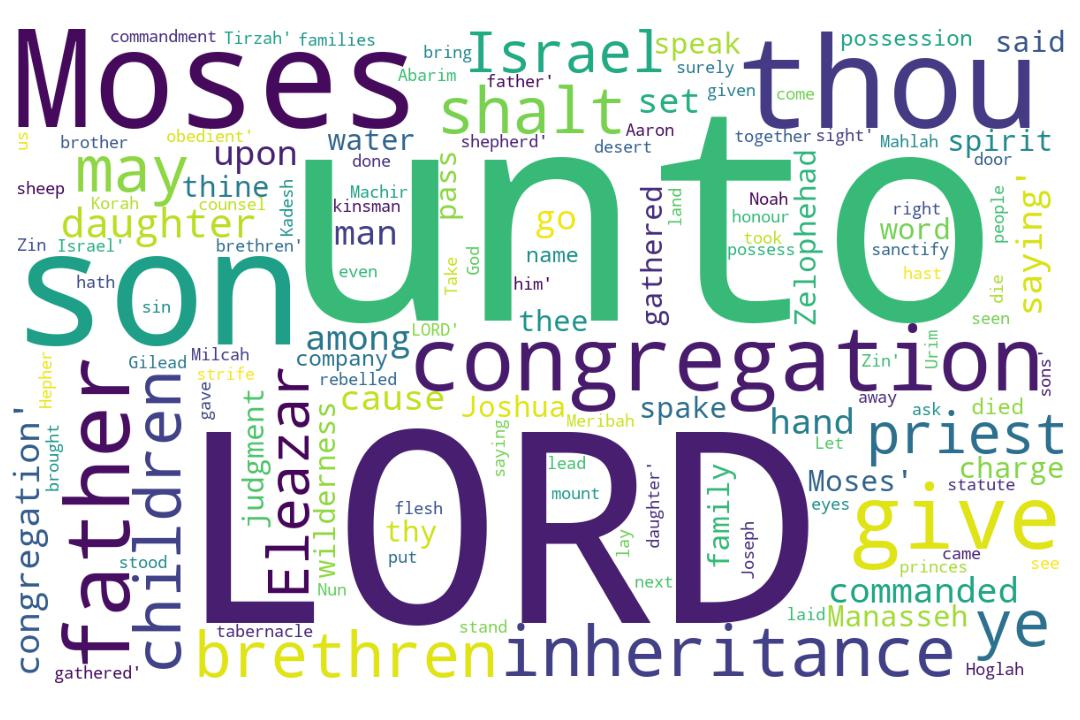
\includegraphics[width=\linewidth]{04OT-Numbers/Numbers27-WordCloud.jpg}
  \caption{Numbers 27 Word Cloud}
  \label{fig:Numbers 27 word Cloud}
\end{figure}

\marginpar{\scriptsize \centering \fcolorbox{blue}{lime}{\textbf{DAUGHTERS OF ZELOPHEHAD}}\\ (Numbers 27)
\begin{compactenum}[I.][8]
    \item \textbf{Single and Dispossessed} \index[scripture]{Numbers!Num 27:01--04} (Numbers 27:2--4)
    \item \textbf{Standing  before the Priests} \index[scripture]{Numbers!Num 27:02} (Numbers 27:2)
    \item A \textbf{Significant Problems} \index[scripture]{Numbers!Num 27:04} (Numbers 27:4)
    \item A \textbf{Sought Possession} \index[scripture]{Numbers!Num 27:04} (Numbers 27:4)
    \item The \textbf{Stated Plan} \index[scripture]{Numbers!Num 27:08--10} (Numbers 27:8--10)
\end{compactenum}}

%%%%%%%%%%%%%%%%%%%%%%%%%%%%%%%%%%
%%%%%%%%%%%%%%%%%%%%%%%%%%%%%%%%%%
\footnote{\textcolor[rgb]{0.00,0.25,0.00}{\hyperlink{TOC}{Return to end of Table of Contents.}}}\footnote{\href{https://audiobible.com/bible/numbers_27.html}{\textcolor[cmyk]{0.99998,1,0,0}{Numbers 27 Audio}}}\textcolor[cmyk]{0.99998,1,0,0}{Then came the daughters of Zelophehad, the son of Hepher, the son of Gilead, the son of Machir, the son of Manasseh, of the families of Manasseh the son of Joseph: and these \emph{are} the names of his daughters; Mahlah, Noah, and Hoglah, and Milcah, and Tirzah.}
[2] \textcolor[cmyk]{0.99998,1,0,0}{And they stood \fcolorbox{bone}{bone}{before} Moses, and \fcolorbox{bone}{bone}{before} Eleazar the priest, and \fcolorbox{bone}{bone}{before} the princes and all the congregation, \emph{by} the door of the tabernacle of the congregation, saying,}
[3] \textcolor[cmyk]{0.99998,1,0,0}{Our father died \fcolorbox{bone}{bone}{in} the wilderness, and he was not \fcolorbox{bone}{bone}{in} the company of them that gathered themselves together against the LORD \fcolorbox{bone}{bone}{in} the company of Korah; but died \fcolorbox{bone}{bone}{in} his own sin, and had no sons.}
[4] \textcolor[cmyk]{0.99998,1,0,0}{Why should the name of our father be done away from among his family, because he hath no son? Give unto us \emph{therefore} a possession among the brethren of our father.}
[5] \textcolor[cmyk]{0.99998,1,0,0}{And Moses brought their cause \fcolorbox{bone}{bone}{before} the LORD.}\\
\\
\P \textcolor[cmyk]{0.99998,1,0,0}{And the LORD spake unto Moses, saying,}
[7] \textcolor[cmyk]{0.99998,1,0,0}{The daughters of Zelophehad speak right: thou shalt surely give them a possession of an inheritance among their father's brethren; and thou shalt cause the inheritance of their father to pass unto them.}
[8] \textcolor[cmyk]{0.99998,1,0,0}{And thou shalt speak unto the children of Israel, saying, If a man die, and have no son, then ye shall cause his inheritance to pass unto his daughter.}
[9] \textcolor[cmyk]{0.99998,1,0,0}{And if he have no daughter, then ye shall give his inheritance unto his brethren.}
[10] \textcolor[cmyk]{0.99998,1,0,0}{And if he have no brethren, then ye shall give his inheritance unto his father's brethren.}
[11] \textcolor[cmyk]{0.99998,1,0,0}{And if his father have no brethren, then ye shall give his inheritance unto his kinsman that is next to him of his family, and he shall possess it: and it shall be unto the children of Israel a statute of judgment, as the LORD commanded Moses.}\\
\\
\P \textcolor[cmyk]{0.99998,1,0,0}{And the LORD said unto Moses, Get thee up into this mount Abarim, and see the land which I have given unto the children of Israel.}
[13] \textcolor[cmyk]{0.99998,1,0,0}{And when thou hast seen it, thou also shalt be gathered unto thy people, as Aaron thy brother was gathered.}
[14] \textcolor[cmyk]{0.99998,1,0,0}{For ye rebelled against my commandment \fcolorbox{bone}{bone}{in} the desert of Zin, \fcolorbox{bone}{bone}{in} the strife of the congregation, to sanctify me at the water \fcolorbox{bone}{bone}{before} their eyes: that \emph{is} the water of Meribah \fcolorbox{bone}{bone}{in} Kadesh \fcolorbox{bone}{bone}{in} the wilderness of Zin.}\\
\\
\P \textcolor[cmyk]{0.99998,1,0,0}{And Moses spake unto the LORD, saying,}
[16] \textcolor[cmyk]{0.99998,1,0,0}{Let the LORD, the God of the spirits of all flesh, set a man over the congregation,}
[17] \textcolor[cmyk]{0.99998,1,0,0}{Which may go out \fcolorbox{bone}{bone}{before} them, and which may go \fcolorbox{bone}{bone}{in} \fcolorbox{bone}{bone}{before} them, and which may lead them out, and which may bring them \fcolorbox{bone}{bone}{in}; that the congregation of the LORD be not as sheep which have no shepherd.}\\
\\
\P \textcolor[cmyk]{0.99998,1,0,0}{And the LORD said unto Moses, Take thee Joshua the son of Nun, a man \fcolorbox{bone}{bone}{in} whom \emph{is} the spirit, and lay thine hand upon him;}
[19] \textcolor[cmyk]{0.99998,1,0,0}{And set him \fcolorbox{bone}{bone}{before} Eleazar the priest, and \fcolorbox{bone}{bone}{before} all the congregation; and give him a charge \fcolorbox{bone}{bone}{in} their sight.}
[20] \textcolor[cmyk]{0.99998,1,0,0}{And thou shalt put \emph{some} of thine honour upon him, that all the congregation of the children of Israel may be obedient.}
[21] \textcolor[cmyk]{0.99998,1,0,0}{And he shall stand \fcolorbox{bone}{bone}{before} Eleazar the priest, who shall ask \emph{counsel} for him after the judgment of Urim \fcolorbox{bone}{bone}{before} the LORD: at his word shall they go out, and at his word they shall come \fcolorbox{bone}{bone}{in}, \emph{both} he, and all the children of Israel with him, even all the congregation.}
[22] \textcolor[cmyk]{0.99998,1,0,0}{And Moses did as the LORD commanded him: and he took Joshua, and set him \fcolorbox{bone}{bone}{before} Eleazar the priest, and \fcolorbox{bone}{bone}{before} all the congregation:}
[23] \textcolor[cmyk]{0.99998,1,0,0}{And he laid his hand upon him, and gave him a charge, as the LORD commanded by the hand of Moses.}
\index[NWIV]{47!Numbers!Num 27:1}\index[AWIP]{Then!Numbers!Num 27:1}\index[AWIP]{came!Numbers!Num 27:1}\index[AWIP]{the!Numbers!Num 27:1}\index[AWIP]{the!Numbers!Num 27:1 (2)}\index[AWIP]{the!Numbers!Num 27:1 (3)}\index[AWIP]{the!Numbers!Num 27:1 (4)}\index[AWIP]{the!Numbers!Num 27:1 (5)}\index[AWIP]{the!Numbers!Num 27:1 (6)}\index[AWIP]{the!Numbers!Num 27:1 (7)}\index[AWIP]{the!Numbers!Num 27:1 (8)}\index[AWIP]{daughters!Numbers!Num 27:1}\index[AWIP]{daughters!Numbers!Num 27:1 (2)}\index[AWIP]{of!Numbers!Num 27:1}\index[AWIP]{of!Numbers!Num 27:1 (2)}\index[AWIP]{of!Numbers!Num 27:1 (3)}\index[AWIP]{of!Numbers!Num 27:1 (4)}\index[AWIP]{of!Numbers!Num 27:1 (5)}\index[AWIP]{of!Numbers!Num 27:1 (6)}\index[AWIP]{of!Numbers!Num 27:1 (7)}\index[AWIP]{of!Numbers!Num 27:1 (8)}\index[AWIP]{of!Numbers!Num 27:1 (9)}\index[AWIP]{Zelophehad!Numbers!Num 27:1}\index[AWIP]{son!Numbers!Num 27:1}\index[AWIP]{son!Numbers!Num 27:1 (2)}\index[AWIP]{son!Numbers!Num 27:1 (3)}\index[AWIP]{son!Numbers!Num 27:1 (4)}\index[AWIP]{son!Numbers!Num 27:1 (5)}\index[AWIP]{Hepher!Numbers!Num 27:1}\index[AWIP]{Gilead!Numbers!Num 27:1}\index[AWIP]{Machir!Numbers!Num 27:1}\index[AWIP]{Manasseh!Numbers!Num 27:1}\index[AWIP]{Manasseh!Numbers!Num 27:1 (2)}\index[AWIP]{families!Numbers!Num 27:1}\index[AWIP]{Joseph!Numbers!Num 27:1}\index[AWIP]{and!Numbers!Num 27:1}\index[AWIP]{and!Numbers!Num 27:1 (2)}\index[AWIP]{and!Numbers!Num 27:1 (3)}\index[AWIP]{and!Numbers!Num 27:1 (4)}\index[AWIP]{these!Numbers!Num 27:1}\index[AWIP]{\emph{are}!Numbers!Num 27:1}\index[AWIP]{names!Numbers!Num 27:1}\index[AWIP]{his!Numbers!Num 27:1}\index[AWIP]{Mahlah!Numbers!Num 27:1}\index[AWIP]{Noah!Numbers!Num 27:1}\index[AWIP]{Hoglah!Numbers!Num 27:1}\index[AWIP]{Milcah!Numbers!Num 27:1}\index[AWIP]{Tirzah!Numbers!Num 27:1}\index[AWIP]{\emph{are}!Numbers!Num 27:1}

\index[NWIV]{28!Numbers!Num 27:2}\index[AWIP]{And!Numbers!Num 27:2}\index[AWIP]{they!Numbers!Num 27:2}\index[AWIP]{stood!Numbers!Num 27:2}\index[AWIP]{before!Numbers!Num 27:2}\index[AWIP]{before!Numbers!Num 27:2 (2)}\index[AWIP]{before!Numbers!Num 27:2 (3)}\index[AWIP]{Moses!Numbers!Num 27:2}\index[AWIP]{and!Numbers!Num 27:2}\index[AWIP]{and!Numbers!Num 27:2 (2)}\index[AWIP]{and!Numbers!Num 27:2 (3)}\index[AWIP]{Eleazar!Numbers!Num 27:2}\index[AWIP]{the!Numbers!Num 27:2}\index[AWIP]{the!Numbers!Num 27:2 (2)}\index[AWIP]{the!Numbers!Num 27:2 (3)}\index[AWIP]{the!Numbers!Num 27:2 (4)}\index[AWIP]{the!Numbers!Num 27:2 (5)}\index[AWIP]{the!Numbers!Num 27:2 (6)}\index[AWIP]{priest!Numbers!Num 27:2}\index[AWIP]{princes!Numbers!Num 27:2}\index[AWIP]{all!Numbers!Num 27:2}\index[AWIP]{congregation!Numbers!Num 27:2}\index[AWIP]{congregation!Numbers!Num 27:2 (2)}\index[AWIP]{\emph{by}!Numbers!Num 27:2}\index[AWIP]{door!Numbers!Num 27:2}\index[AWIP]{of!Numbers!Num 27:2}\index[AWIP]{of!Numbers!Num 27:2 (2)}\index[AWIP]{tabernacle!Numbers!Num 27:2}\index[AWIP]{saying!Numbers!Num 27:2}\index[AWIP]{\emph{by}!Numbers!Num 27:2}

\index[NWIV]{37!Numbers!Num 27:3}\index[AWIP]{Our!Numbers!Num 27:3}\index[AWIP]{father!Numbers!Num 27:3}\index[AWIP]{died!Numbers!Num 27:3}\index[AWIP]{died!Numbers!Num 27:3 (2)}\index[AWIP]{in!Numbers!Num 27:3}\index[AWIP]{in!Numbers!Num 27:3 (2)}\index[AWIP]{in!Numbers!Num 27:3 (3)}\index[AWIP]{in!Numbers!Num 27:3 (4)}\index[AWIP]{the!Numbers!Num 27:3}\index[AWIP]{the!Numbers!Num 27:3 (2)}\index[AWIP]{the!Numbers!Num 27:3 (3)}\index[AWIP]{the!Numbers!Num 27:3 (4)}\index[AWIP]{wilderness!Numbers!Num 27:3}\index[AWIP]{and!Numbers!Num 27:3}\index[AWIP]{and!Numbers!Num 27:3 (2)}\index[AWIP]{he!Numbers!Num 27:3}\index[AWIP]{was!Numbers!Num 27:3}\index[AWIP]{not!Numbers!Num 27:3}\index[AWIP]{company!Numbers!Num 27:3}\index[AWIP]{company!Numbers!Num 27:3 (2)}\index[AWIP]{of!Numbers!Num 27:3}\index[AWIP]{of!Numbers!Num 27:3 (2)}\index[AWIP]{them!Numbers!Num 27:3}\index[AWIP]{that!Numbers!Num 27:3}\index[AWIP]{gathered!Numbers!Num 27:3}\index[AWIP]{themselves!Numbers!Num 27:3}\index[AWIP]{together!Numbers!Num 27:3}\index[AWIP]{against!Numbers!Num 27:3}\index[AWIP]{LORD!Numbers!Num 27:3}\index[AWIP]{Korah!Numbers!Num 27:3}\index[AWIP]{but!Numbers!Num 27:3}\index[AWIP]{his!Numbers!Num 27:3}\index[AWIP]{own!Numbers!Num 27:3}\index[AWIP]{sin!Numbers!Num 27:3}\index[AWIP]{had!Numbers!Num 27:3}\index[AWIP]{no!Numbers!Num 27:3}\index[AWIP]{sons!Numbers!Num 27:3}

\index[NWIV]{31!Numbers!Num 27:4}\index[AWIP]{Why!Numbers!Num 27:4}\index[AWIP]{should!Numbers!Num 27:4}\index[AWIP]{the!Numbers!Num 27:4}\index[AWIP]{the!Numbers!Num 27:4 (2)}\index[AWIP]{name!Numbers!Num 27:4}\index[AWIP]{of!Numbers!Num 27:4}\index[AWIP]{of!Numbers!Num 27:4 (2)}\index[AWIP]{our!Numbers!Num 27:4}\index[AWIP]{our!Numbers!Num 27:4 (2)}\index[AWIP]{father!Numbers!Num 27:4}\index[AWIP]{father!Numbers!Num 27:4 (2)}\index[AWIP]{be!Numbers!Num 27:4}\index[AWIP]{done!Numbers!Num 27:4}\index[AWIP]{away!Numbers!Num 27:4}\index[AWIP]{from!Numbers!Num 27:4}\index[AWIP]{among!Numbers!Num 27:4}\index[AWIP]{among!Numbers!Num 27:4 (2)}\index[AWIP]{his!Numbers!Num 27:4}\index[AWIP]{family!Numbers!Num 27:4}\index[AWIP]{because!Numbers!Num 27:4}\index[AWIP]{he!Numbers!Num 27:4}\index[AWIP]{hath!Numbers!Num 27:4}\index[AWIP]{no!Numbers!Num 27:4}\index[AWIP]{son?!Numbers!Num 27:4}\index[AWIP]{Give!Numbers!Num 27:4}\index[AWIP]{unto!Numbers!Num 27:4}\index[AWIP]{us!Numbers!Num 27:4}\index[AWIP]{\emph{therefore}!Numbers!Num 27:4}\index[AWIP]{a!Numbers!Num 27:4}\index[AWIP]{possession!Numbers!Num 27:4}\index[AWIP]{brethren!Numbers!Num 27:4}\index[AWIP]{\emph{therefore}!Numbers!Num 27:4}

\index[NWIV]{8!Numbers!Num 27:5}\index[AWIP]{And!Numbers!Num 27:5}\index[AWIP]{Moses!Numbers!Num 27:5}\index[AWIP]{brought!Numbers!Num 27:5}\index[AWIP]{their!Numbers!Num 27:5}\index[AWIP]{cause!Numbers!Num 27:5}\index[AWIP]{before!Numbers!Num 27:5}\index[AWIP]{the!Numbers!Num 27:5}\index[AWIP]{LORD!Numbers!Num 27:5}

\index[NWIV]{7!Numbers!Num 27:6}\index[AWIP]{And!Numbers!Num 27:6}\index[AWIP]{the!Numbers!Num 27:6}\index[AWIP]{LORD!Numbers!Num 27:6}\index[AWIP]{spake!Numbers!Num 27:6}\index[AWIP]{unto!Numbers!Num 27:6}\index[AWIP]{Moses!Numbers!Num 27:6}\index[AWIP]{saying!Numbers!Num 27:6}

\index[NWIV]{33!Numbers!Num 27:7}\index[AWIP]{The!Numbers!Num 27:7}\index[AWIP]{daughters!Numbers!Num 27:7}\index[AWIP]{of!Numbers!Num 27:7}\index[AWIP]{of!Numbers!Num 27:7 (2)}\index[AWIP]{of!Numbers!Num 27:7 (3)}\index[AWIP]{Zelophehad!Numbers!Num 27:7}\index[AWIP]{speak!Numbers!Num 27:7}\index[AWIP]{right!Numbers!Num 27:7}\index[AWIP]{thou!Numbers!Num 27:7}\index[AWIP]{thou!Numbers!Num 27:7 (2)}\index[AWIP]{shalt!Numbers!Num 27:7}\index[AWIP]{shalt!Numbers!Num 27:7 (2)}\index[AWIP]{surely!Numbers!Num 27:7}\index[AWIP]{give!Numbers!Num 27:7}\index[AWIP]{them!Numbers!Num 27:7}\index[AWIP]{them!Numbers!Num 27:7 (2)}\index[AWIP]{a!Numbers!Num 27:7}\index[AWIP]{possession!Numbers!Num 27:7}\index[AWIP]{an!Numbers!Num 27:7}\index[AWIP]{inheritance!Numbers!Num 27:7}\index[AWIP]{inheritance!Numbers!Num 27:7 (2)}\index[AWIP]{among!Numbers!Num 27:7}\index[AWIP]{their!Numbers!Num 27:7}\index[AWIP]{their!Numbers!Num 27:7 (2)}\index[AWIP]{father's!Numbers!Num 27:7}\index[AWIP]{brethren!Numbers!Num 27:7}\index[AWIP]{and!Numbers!Num 27:7}\index[AWIP]{cause!Numbers!Num 27:7}\index[AWIP]{the!Numbers!Num 27:7}\index[AWIP]{father!Numbers!Num 27:7}\index[AWIP]{to!Numbers!Num 27:7}\index[AWIP]{pass!Numbers!Num 27:7}\index[AWIP]{unto!Numbers!Num 27:7}

\index[NWIV]{29!Numbers!Num 27:8}\index[AWIP]{And!Numbers!Num 27:8}\index[AWIP]{thou!Numbers!Num 27:8}\index[AWIP]{shalt!Numbers!Num 27:8}\index[AWIP]{speak!Numbers!Num 27:8}\index[AWIP]{unto!Numbers!Num 27:8}\index[AWIP]{unto!Numbers!Num 27:8 (2)}\index[AWIP]{the!Numbers!Num 27:8}\index[AWIP]{children!Numbers!Num 27:8}\index[AWIP]{of!Numbers!Num 27:8}\index[AWIP]{Israel!Numbers!Num 27:8}\index[AWIP]{saying!Numbers!Num 27:8}\index[AWIP]{If!Numbers!Num 27:8}\index[AWIP]{a!Numbers!Num 27:8}\index[AWIP]{man!Numbers!Num 27:8}\index[AWIP]{die!Numbers!Num 27:8}\index[AWIP]{and!Numbers!Num 27:8}\index[AWIP]{have!Numbers!Num 27:8}\index[AWIP]{no!Numbers!Num 27:8}\index[AWIP]{son!Numbers!Num 27:8}\index[AWIP]{then!Numbers!Num 27:8}\index[AWIP]{ye!Numbers!Num 27:8}\index[AWIP]{shall!Numbers!Num 27:8}\index[AWIP]{cause!Numbers!Num 27:8}\index[AWIP]{his!Numbers!Num 27:8}\index[AWIP]{his!Numbers!Num 27:8 (2)}\index[AWIP]{inheritance!Numbers!Num 27:8}\index[AWIP]{to!Numbers!Num 27:8}\index[AWIP]{pass!Numbers!Num 27:8}\index[AWIP]{daughter!Numbers!Num 27:8}

\index[NWIV]{15!Numbers!Num 27:9}\index[AWIP]{And!Numbers!Num 27:9}\index[AWIP]{if!Numbers!Num 27:9}\index[AWIP]{he!Numbers!Num 27:9}\index[AWIP]{have!Numbers!Num 27:9}\index[AWIP]{no!Numbers!Num 27:9}\index[AWIP]{daughter!Numbers!Num 27:9}\index[AWIP]{then!Numbers!Num 27:9}\index[AWIP]{ye!Numbers!Num 27:9}\index[AWIP]{shall!Numbers!Num 27:9}\index[AWIP]{give!Numbers!Num 27:9}\index[AWIP]{his!Numbers!Num 27:9}\index[AWIP]{his!Numbers!Num 27:9 (2)}\index[AWIP]{inheritance!Numbers!Num 27:9}\index[AWIP]{unto!Numbers!Num 27:9}\index[AWIP]{brethren!Numbers!Num 27:9}

\index[NWIV]{16!Numbers!Num 27:10}\index[AWIP]{And!Numbers!Num 27:10}\index[AWIP]{if!Numbers!Num 27:10}\index[AWIP]{he!Numbers!Num 27:10}\index[AWIP]{have!Numbers!Num 27:10}\index[AWIP]{no!Numbers!Num 27:10}\index[AWIP]{brethren!Numbers!Num 27:10}\index[AWIP]{brethren!Numbers!Num 27:10 (2)}\index[AWIP]{then!Numbers!Num 27:10}\index[AWIP]{ye!Numbers!Num 27:10}\index[AWIP]{shall!Numbers!Num 27:10}\index[AWIP]{give!Numbers!Num 27:10}\index[AWIP]{his!Numbers!Num 27:10}\index[AWIP]{his!Numbers!Num 27:10 (2)}\index[AWIP]{inheritance!Numbers!Num 27:10}\index[AWIP]{unto!Numbers!Num 27:10}\index[AWIP]{father's!Numbers!Num 27:10}

\index[NWIV]{47!Numbers!Num 27:11}\index[AWIP]{And!Numbers!Num 27:11}\index[AWIP]{if!Numbers!Num 27:11}\index[AWIP]{his!Numbers!Num 27:11}\index[AWIP]{his!Numbers!Num 27:11 (2)}\index[AWIP]{his!Numbers!Num 27:11 (3)}\index[AWIP]{his!Numbers!Num 27:11 (4)}\index[AWIP]{father!Numbers!Num 27:11}\index[AWIP]{have!Numbers!Num 27:11}\index[AWIP]{no!Numbers!Num 27:11}\index[AWIP]{brethren!Numbers!Num 27:11}\index[AWIP]{then!Numbers!Num 27:11}\index[AWIP]{ye!Numbers!Num 27:11}\index[AWIP]{shall!Numbers!Num 27:11}\index[AWIP]{shall!Numbers!Num 27:11 (2)}\index[AWIP]{shall!Numbers!Num 27:11 (3)}\index[AWIP]{give!Numbers!Num 27:11}\index[AWIP]{inheritance!Numbers!Num 27:11}\index[AWIP]{unto!Numbers!Num 27:11}\index[AWIP]{unto!Numbers!Num 27:11 (2)}\index[AWIP]{kinsman!Numbers!Num 27:11}\index[AWIP]{that!Numbers!Num 27:11}\index[AWIP]{is!Numbers!Num 27:11}\index[AWIP]{next!Numbers!Num 27:11}\index[AWIP]{to!Numbers!Num 27:11}\index[AWIP]{him!Numbers!Num 27:11}\index[AWIP]{of!Numbers!Num 27:11}\index[AWIP]{of!Numbers!Num 27:11 (2)}\index[AWIP]{of!Numbers!Num 27:11 (3)}\index[AWIP]{family!Numbers!Num 27:11}\index[AWIP]{and!Numbers!Num 27:11}\index[AWIP]{and!Numbers!Num 27:11 (2)}\index[AWIP]{he!Numbers!Num 27:11}\index[AWIP]{possess!Numbers!Num 27:11}\index[AWIP]{it!Numbers!Num 27:11}\index[AWIP]{it!Numbers!Num 27:11 (2)}\index[AWIP]{be!Numbers!Num 27:11}\index[AWIP]{the!Numbers!Num 27:11}\index[AWIP]{the!Numbers!Num 27:11 (2)}\index[AWIP]{children!Numbers!Num 27:11}\index[AWIP]{Israel!Numbers!Num 27:11}\index[AWIP]{a!Numbers!Num 27:11}\index[AWIP]{statute!Numbers!Num 27:11}\index[AWIP]{judgment!Numbers!Num 27:11}\index[AWIP]{as!Numbers!Num 27:11}\index[AWIP]{LORD!Numbers!Num 27:11}\index[AWIP]{commanded!Numbers!Num 27:11}\index[AWIP]{Moses!Numbers!Num 27:11}

\index[NWIV]{26!Numbers!Num 27:12}\index[AWIP]{And!Numbers!Num 27:12}\index[AWIP]{the!Numbers!Num 27:12}\index[AWIP]{the!Numbers!Num 27:12 (2)}\index[AWIP]{the!Numbers!Num 27:12 (3)}\index[AWIP]{LORD!Numbers!Num 27:12}\index[AWIP]{said!Numbers!Num 27:12}\index[AWIP]{unto!Numbers!Num 27:12}\index[AWIP]{unto!Numbers!Num 27:12 (2)}\index[AWIP]{Moses!Numbers!Num 27:12}\index[AWIP]{Get!Numbers!Num 27:12}\index[AWIP]{thee!Numbers!Num 27:12}\index[AWIP]{up!Numbers!Num 27:12}\index[AWIP]{into!Numbers!Num 27:12}\index[AWIP]{this!Numbers!Num 27:12}\index[AWIP]{mount!Numbers!Num 27:12}\index[AWIP]{Abarim!Numbers!Num 27:12}\index[AWIP]{and!Numbers!Num 27:12}\index[AWIP]{see!Numbers!Num 27:12}\index[AWIP]{land!Numbers!Num 27:12}\index[AWIP]{which!Numbers!Num 27:12}\index[AWIP]{I!Numbers!Num 27:12}\index[AWIP]{have!Numbers!Num 27:12}\index[AWIP]{given!Numbers!Num 27:12}\index[AWIP]{children!Numbers!Num 27:12}\index[AWIP]{of!Numbers!Num 27:12}\index[AWIP]{Israel!Numbers!Num 27:12}

\index[NWIV]{20!Numbers!Num 27:13}\index[AWIP]{And!Numbers!Num 27:13}\index[AWIP]{when!Numbers!Num 27:13}\index[AWIP]{thou!Numbers!Num 27:13}\index[AWIP]{thou!Numbers!Num 27:13 (2)}\index[AWIP]{hast!Numbers!Num 27:13}\index[AWIP]{seen!Numbers!Num 27:13}\index[AWIP]{it!Numbers!Num 27:13}\index[AWIP]{also!Numbers!Num 27:13}\index[AWIP]{shalt!Numbers!Num 27:13}\index[AWIP]{be!Numbers!Num 27:13}\index[AWIP]{gathered!Numbers!Num 27:13}\index[AWIP]{gathered!Numbers!Num 27:13 (2)}\index[AWIP]{unto!Numbers!Num 27:13}\index[AWIP]{thy!Numbers!Num 27:13}\index[AWIP]{thy!Numbers!Num 27:13 (2)}\index[AWIP]{people!Numbers!Num 27:13}\index[AWIP]{as!Numbers!Num 27:13}\index[AWIP]{Aaron!Numbers!Num 27:13}\index[AWIP]{brother!Numbers!Num 27:13}\index[AWIP]{was!Numbers!Num 27:13}

\index[NWIV]{39!Numbers!Num 27:14}\index[AWIP]{For!Numbers!Num 27:14}\index[AWIP]{ye!Numbers!Num 27:14}\index[AWIP]{rebelled!Numbers!Num 27:14}\index[AWIP]{against!Numbers!Num 27:14}\index[AWIP]{my!Numbers!Num 27:14}\index[AWIP]{commandment!Numbers!Num 27:14}\index[AWIP]{in!Numbers!Num 27:14}\index[AWIP]{in!Numbers!Num 27:14 (2)}\index[AWIP]{in!Numbers!Num 27:14 (3)}\index[AWIP]{in!Numbers!Num 27:14 (4)}\index[AWIP]{the!Numbers!Num 27:14}\index[AWIP]{the!Numbers!Num 27:14 (2)}\index[AWIP]{the!Numbers!Num 27:14 (3)}\index[AWIP]{the!Numbers!Num 27:14 (4)}\index[AWIP]{the!Numbers!Num 27:14 (5)}\index[AWIP]{the!Numbers!Num 27:14 (6)}\index[AWIP]{desert!Numbers!Num 27:14}\index[AWIP]{of!Numbers!Num 27:14}\index[AWIP]{of!Numbers!Num 27:14 (2)}\index[AWIP]{of!Numbers!Num 27:14 (3)}\index[AWIP]{of!Numbers!Num 27:14 (4)}\index[AWIP]{Zin!Numbers!Num 27:14}\index[AWIP]{Zin!Numbers!Num 27:14 (2)}\index[AWIP]{strife!Numbers!Num 27:14}\index[AWIP]{congregation!Numbers!Num 27:14}\index[AWIP]{to!Numbers!Num 27:14}\index[AWIP]{sanctify!Numbers!Num 27:14}\index[AWIP]{me!Numbers!Num 27:14}\index[AWIP]{at!Numbers!Num 27:14}\index[AWIP]{water!Numbers!Num 27:14}\index[AWIP]{water!Numbers!Num 27:14 (2)}\index[AWIP]{before!Numbers!Num 27:14}\index[AWIP]{their!Numbers!Num 27:14}\index[AWIP]{eyes!Numbers!Num 27:14}\index[AWIP]{that!Numbers!Num 27:14}\index[AWIP]{\emph{is}!Numbers!Num 27:14}\index[AWIP]{Meribah!Numbers!Num 27:14}\index[AWIP]{Kadesh!Numbers!Num 27:14}\index[AWIP]{wilderness!Numbers!Num 27:14}\index[AWIP]{\emph{is}!Numbers!Num 27:14}

\index[NWIV]{7!Numbers!Num 27:15}\index[AWIP]{And!Numbers!Num 27:15}\index[AWIP]{Moses!Numbers!Num 27:15}\index[AWIP]{spake!Numbers!Num 27:15}\index[AWIP]{unto!Numbers!Num 27:15}\index[AWIP]{the!Numbers!Num 27:15}\index[AWIP]{LORD!Numbers!Num 27:15}\index[AWIP]{saying!Numbers!Num 27:15}

\index[NWIV]{17!Numbers!Num 27:16}\index[AWIP]{Let!Numbers!Num 27:16}\index[AWIP]{the!Numbers!Num 27:16}\index[AWIP]{the!Numbers!Num 27:16 (2)}\index[AWIP]{the!Numbers!Num 27:16 (3)}\index[AWIP]{the!Numbers!Num 27:16 (4)}\index[AWIP]{LORD!Numbers!Num 27:16}\index[AWIP]{God!Numbers!Num 27:16}\index[AWIP]{of!Numbers!Num 27:16}\index[AWIP]{of!Numbers!Num 27:16 (2)}\index[AWIP]{spirits!Numbers!Num 27:16}\index[AWIP]{all!Numbers!Num 27:16}\index[AWIP]{flesh!Numbers!Num 27:16}\index[AWIP]{set!Numbers!Num 27:16}\index[AWIP]{a!Numbers!Num 27:16}\index[AWIP]{man!Numbers!Num 27:16}\index[AWIP]{over!Numbers!Num 27:16}\index[AWIP]{congregation!Numbers!Num 27:16}

\index[NWIV]{39!Numbers!Num 27:17}\index[AWIP]{Which!Numbers!Num 27:17}\index[AWIP]{may!Numbers!Num 27:17}\index[AWIP]{may!Numbers!Num 27:17 (2)}\index[AWIP]{may!Numbers!Num 27:17 (3)}\index[AWIP]{may!Numbers!Num 27:17 (4)}\index[AWIP]{go!Numbers!Num 27:17}\index[AWIP]{go!Numbers!Num 27:17 (2)}\index[AWIP]{out!Numbers!Num 27:17}\index[AWIP]{out!Numbers!Num 27:17 (2)}\index[AWIP]{before!Numbers!Num 27:17}\index[AWIP]{before!Numbers!Num 27:17 (2)}\index[AWIP]{them!Numbers!Num 27:17}\index[AWIP]{them!Numbers!Num 27:17 (2)}\index[AWIP]{them!Numbers!Num 27:17 (3)}\index[AWIP]{them!Numbers!Num 27:17 (4)}\index[AWIP]{and!Numbers!Num 27:17}\index[AWIP]{and!Numbers!Num 27:17 (2)}\index[AWIP]{and!Numbers!Num 27:17 (3)}\index[AWIP]{which!Numbers!Num 27:17}\index[AWIP]{which!Numbers!Num 27:17 (2)}\index[AWIP]{which!Numbers!Num 27:17 (3)}\index[AWIP]{which!Numbers!Num 27:17 (4)}\index[AWIP]{in!Numbers!Num 27:17}\index[AWIP]{in!Numbers!Num 27:17 (2)}\index[AWIP]{lead!Numbers!Num 27:17}\index[AWIP]{bring!Numbers!Num 27:17}\index[AWIP]{that!Numbers!Num 27:17}\index[AWIP]{the!Numbers!Num 27:17}\index[AWIP]{the!Numbers!Num 27:17 (2)}\index[AWIP]{congregation!Numbers!Num 27:17}\index[AWIP]{of!Numbers!Num 27:17}\index[AWIP]{LORD!Numbers!Num 27:17}\index[AWIP]{be!Numbers!Num 27:17}\index[AWIP]{not!Numbers!Num 27:17}\index[AWIP]{as!Numbers!Num 27:17}\index[AWIP]{sheep!Numbers!Num 27:17}\index[AWIP]{have!Numbers!Num 27:17}\index[AWIP]{no!Numbers!Num 27:17}\index[AWIP]{shepherd!Numbers!Num 27:17}

\index[NWIV]{26!Numbers!Num 27:18}\index[AWIP]{And!Numbers!Num 27:18}\index[AWIP]{the!Numbers!Num 27:18}\index[AWIP]{the!Numbers!Num 27:18 (2)}\index[AWIP]{the!Numbers!Num 27:18 (3)}\index[AWIP]{LORD!Numbers!Num 27:18}\index[AWIP]{said!Numbers!Num 27:18}\index[AWIP]{unto!Numbers!Num 27:18}\index[AWIP]{Moses!Numbers!Num 27:18}\index[AWIP]{Take!Numbers!Num 27:18}\index[AWIP]{thee!Numbers!Num 27:18}\index[AWIP]{Joshua!Numbers!Num 27:18}\index[AWIP]{son!Numbers!Num 27:18}\index[AWIP]{of!Numbers!Num 27:18}\index[AWIP]{Nun!Numbers!Num 27:18}\index[AWIP]{a!Numbers!Num 27:18}\index[AWIP]{man!Numbers!Num 27:18}\index[AWIP]{in!Numbers!Num 27:18}\index[AWIP]{whom!Numbers!Num 27:18}\index[AWIP]{\emph{is}!Numbers!Num 27:18}\index[AWIP]{spirit!Numbers!Num 27:18}\index[AWIP]{and!Numbers!Num 27:18}\index[AWIP]{lay!Numbers!Num 27:18}\index[AWIP]{thine!Numbers!Num 27:18}\index[AWIP]{hand!Numbers!Num 27:18}\index[AWIP]{upon!Numbers!Num 27:18}\index[AWIP]{him!Numbers!Num 27:18}\index[AWIP]{\emph{is}!Numbers!Num 27:18}

\index[NWIV]{20!Numbers!Num 27:19}\index[AWIP]{And!Numbers!Num 27:19}\index[AWIP]{set!Numbers!Num 27:19}\index[AWIP]{him!Numbers!Num 27:19}\index[AWIP]{him!Numbers!Num 27:19 (2)}\index[AWIP]{before!Numbers!Num 27:19}\index[AWIP]{before!Numbers!Num 27:19 (2)}\index[AWIP]{Eleazar!Numbers!Num 27:19}\index[AWIP]{the!Numbers!Num 27:19}\index[AWIP]{the!Numbers!Num 27:19 (2)}\index[AWIP]{priest!Numbers!Num 27:19}\index[AWIP]{and!Numbers!Num 27:19}\index[AWIP]{and!Numbers!Num 27:19 (2)}\index[AWIP]{all!Numbers!Num 27:19}\index[AWIP]{congregation!Numbers!Num 27:19}\index[AWIP]{give!Numbers!Num 27:19}\index[AWIP]{a!Numbers!Num 27:19}\index[AWIP]{charge!Numbers!Num 27:19}\index[AWIP]{in!Numbers!Num 27:19}\index[AWIP]{their!Numbers!Num 27:19}\index[AWIP]{sight!Numbers!Num 27:19}

\index[NWIV]{22!Numbers!Num 27:20}\index[AWIP]{And!Numbers!Num 27:20}\index[AWIP]{thou!Numbers!Num 27:20}\index[AWIP]{shalt!Numbers!Num 27:20}\index[AWIP]{put!Numbers!Num 27:20}\index[AWIP]{\emph{some}!Numbers!Num 27:20}\index[AWIP]{of!Numbers!Num 27:20}\index[AWIP]{of!Numbers!Num 27:20 (2)}\index[AWIP]{of!Numbers!Num 27:20 (3)}\index[AWIP]{thine!Numbers!Num 27:20}\index[AWIP]{honour!Numbers!Num 27:20}\index[AWIP]{upon!Numbers!Num 27:20}\index[AWIP]{him!Numbers!Num 27:20}\index[AWIP]{that!Numbers!Num 27:20}\index[AWIP]{all!Numbers!Num 27:20}\index[AWIP]{the!Numbers!Num 27:20}\index[AWIP]{the!Numbers!Num 27:20 (2)}\index[AWIP]{congregation!Numbers!Num 27:20}\index[AWIP]{children!Numbers!Num 27:20}\index[AWIP]{Israel!Numbers!Num 27:20}\index[AWIP]{may!Numbers!Num 27:20}\index[AWIP]{be!Numbers!Num 27:20}\index[AWIP]{obedient!Numbers!Num 27:20}\index[AWIP]{\emph{some}!Numbers!Num 27:20}

\index[NWIV]{51!Numbers!Num 27:21}\index[AWIP]{And!Numbers!Num 27:21}\index[AWIP]{he!Numbers!Num 27:21}\index[AWIP]{he!Numbers!Num 27:21 (2)}\index[AWIP]{shall!Numbers!Num 27:21}\index[AWIP]{shall!Numbers!Num 27:21 (2)}\index[AWIP]{shall!Numbers!Num 27:21 (3)}\index[AWIP]{shall!Numbers!Num 27:21 (4)}\index[AWIP]{stand!Numbers!Num 27:21}\index[AWIP]{before!Numbers!Num 27:21}\index[AWIP]{before!Numbers!Num 27:21 (2)}\index[AWIP]{Eleazar!Numbers!Num 27:21}\index[AWIP]{the!Numbers!Num 27:21}\index[AWIP]{the!Numbers!Num 27:21 (2)}\index[AWIP]{the!Numbers!Num 27:21 (3)}\index[AWIP]{the!Numbers!Num 27:21 (4)}\index[AWIP]{the!Numbers!Num 27:21 (5)}\index[AWIP]{priest!Numbers!Num 27:21}\index[AWIP]{who!Numbers!Num 27:21}\index[AWIP]{ask!Numbers!Num 27:21}\index[AWIP]{\emph{counsel}!Numbers!Num 27:21}\index[AWIP]{for!Numbers!Num 27:21}\index[AWIP]{him!Numbers!Num 27:21}\index[AWIP]{him!Numbers!Num 27:21 (2)}\index[AWIP]{after!Numbers!Num 27:21}\index[AWIP]{judgment!Numbers!Num 27:21}\index[AWIP]{of!Numbers!Num 27:21}\index[AWIP]{of!Numbers!Num 27:21 (2)}\index[AWIP]{Urim!Numbers!Num 27:21}\index[AWIP]{LORD!Numbers!Num 27:21}\index[AWIP]{at!Numbers!Num 27:21}\index[AWIP]{at!Numbers!Num 27:21 (2)}\index[AWIP]{his!Numbers!Num 27:21}\index[AWIP]{his!Numbers!Num 27:21 (2)}\index[AWIP]{word!Numbers!Num 27:21}\index[AWIP]{word!Numbers!Num 27:21 (2)}\index[AWIP]{they!Numbers!Num 27:21}\index[AWIP]{they!Numbers!Num 27:21 (2)}\index[AWIP]{go!Numbers!Num 27:21}\index[AWIP]{out!Numbers!Num 27:21}\index[AWIP]{and!Numbers!Num 27:21}\index[AWIP]{and!Numbers!Num 27:21 (2)}\index[AWIP]{come!Numbers!Num 27:21}\index[AWIP]{in!Numbers!Num 27:21}\index[AWIP]{\emph{both}!Numbers!Num 27:21}\index[AWIP]{all!Numbers!Num 27:21}\index[AWIP]{all!Numbers!Num 27:21 (2)}\index[AWIP]{children!Numbers!Num 27:21}\index[AWIP]{Israel!Numbers!Num 27:21}\index[AWIP]{with!Numbers!Num 27:21}\index[AWIP]{even!Numbers!Num 27:21}\index[AWIP]{congregation!Numbers!Num 27:21}\index[AWIP]{\emph{counsel}!Numbers!Num 27:21}\index[AWIP]{\emph{both}!Numbers!Num 27:21}

\index[NWIV]{24!Numbers!Num 27:22}\index[AWIP]{And!Numbers!Num 27:22}\index[AWIP]{Moses!Numbers!Num 27:22}\index[AWIP]{did!Numbers!Num 27:22}\index[AWIP]{as!Numbers!Num 27:22}\index[AWIP]{the!Numbers!Num 27:22}\index[AWIP]{the!Numbers!Num 27:22 (2)}\index[AWIP]{the!Numbers!Num 27:22 (3)}\index[AWIP]{LORD!Numbers!Num 27:22}\index[AWIP]{commanded!Numbers!Num 27:22}\index[AWIP]{him!Numbers!Num 27:22}\index[AWIP]{him!Numbers!Num 27:22 (2)}\index[AWIP]{and!Numbers!Num 27:22}\index[AWIP]{and!Numbers!Num 27:22 (2)}\index[AWIP]{and!Numbers!Num 27:22 (3)}\index[AWIP]{he!Numbers!Num 27:22}\index[AWIP]{took!Numbers!Num 27:22}\index[AWIP]{Joshua!Numbers!Num 27:22}\index[AWIP]{set!Numbers!Num 27:22}\index[AWIP]{before!Numbers!Num 27:22}\index[AWIP]{before!Numbers!Num 27:22 (2)}\index[AWIP]{Eleazar!Numbers!Num 27:22}\index[AWIP]{priest!Numbers!Num 27:22}\index[AWIP]{all!Numbers!Num 27:22}\index[AWIP]{congregation!Numbers!Num 27:22}

\index[NWIV]{21!Numbers!Num 27:23}\index[AWIP]{And!Numbers!Num 27:23}\index[AWIP]{he!Numbers!Num 27:23}\index[AWIP]{laid!Numbers!Num 27:23}\index[AWIP]{his!Numbers!Num 27:23}\index[AWIP]{hands!Numbers!Num 27:23}\index[AWIP]{upon!Numbers!Num 27:23}\index[AWIP]{him!Numbers!Num 27:23}\index[AWIP]{him!Numbers!Num 27:23 (2)}\index[AWIP]{and!Numbers!Num 27:23}\index[AWIP]{gave!Numbers!Num 27:23}\index[AWIP]{a!Numbers!Num 27:23}\index[AWIP]{charge!Numbers!Num 27:23}\index[AWIP]{as!Numbers!Num 27:23}\index[AWIP]{the!Numbers!Num 27:23}\index[AWIP]{the!Numbers!Num 27:23 (2)}\index[AWIP]{LORD!Numbers!Num 27:23}\index[AWIP]{commanded!Numbers!Num 27:23}\index[AWIP]{by!Numbers!Num 27:23}\index[AWIP]{hand!Numbers!Num 27:23}\index[AWIP]{of!Numbers!Num 27:23}\index[AWIP]{Moses!Numbers!Num 27:23}


\section{Numbers 27 Outlines}

\subsection{My Outlines}

\subsubsection{The Daughters of Zelophehad}
\index[speaker]{Keith Anthony!Numbers 27 (The Daughters of Zelophehad)}
\index[series]{Numbers (Keith Anthony)!Numbers 27 (The Daughters of Zelophehad)}
\index[date]{2017/02/18!Numbers 27 (The Daughters of Zelophehad) (Keith Anthony)}
\begin{compactenum}[I.][7]
    \item \textbf{Single and Dispossessed} \index[scripture]{Numbers!Num 27:01--04} (Numbers 27:2--4)
    \item \textbf{Standing before the Priests} \index[scripture]{Numbers!Num 27:02} (Numbers 27:2)
    \item A \textbf{Significant Problems} \index[scripture]{Numbers!Num 27:04} (Numbers 27:4)
    \item A \textbf{Sought Possession} \index[scripture]{Numbers!Num 27:04} (Numbers 27:4)
    \item The \textbf{Stated Plan} \index[scripture]{Numbers!Num 27:08--10} (Numbers 27:8--10)
\end{compactenum}

\subsection{Outlines from Others}



\section{Numbers 27 Comments}

\subsection{Numeric Nuggets}
\textbf{13: } Verse 16 has 13 unique words. The words ``before'' and ``in'' are used 13 times in the chapter.


\subsection{Numbers 27 Repeated Phrases}


%%%%%%%%%%
%%%%%%%%%%
\normalsize
 
\begin{center}
\begin{longtable}{|p{3.0in}|p{0.5in}|}
\caption[Numbers 27 Repeated Phrases]{Numbers 27 Repeated Phrases}\label{table:Repeated Phrases Numbers 27} \\
\hline \multicolumn{1}{|c|}{\textbf{Phrase}} & \multicolumn{1}{c|}{\textbf{Frequency}} \\ \hline 
\endfirsthead
 
\multicolumn{2}{c}
{{\bfseries \tablename\ \thetable{} -- continued from previous page}} \\  
\hline \multicolumn{1}{|c|}{\textbf{Phrase}} & \multicolumn{1}{c|}{\textbf{Frequency}} \\ \hline 
\endhead
 
\hline \multicolumn{2}{c}{{ }} \\ \hline
\endfoot 
the LORD & 12\\ \hline 
the congregation & 9\\ \hline 
of the & 7\\ \hline 
the son & 6\\ \hline 
the son of & 6\\ \hline 
son of & 6\\ \hline 
all the & 6\\ \hline 
in the & 6\\ \hline 
all the congregation & 5\\ \hline 
the children & 5\\ \hline 
the children of & 5\\ \hline 
the children of Israel & 5\\ \hline 
children of & 5\\ \hline 
children of Israel & 5\\ \hline 
of Israel & 5\\ \hline 
have no & 5\\ \hline 
and before & 4\\ \hline 
before Eleazar & 4\\ \hline 
before Eleazar the & 4\\ \hline 
before Eleazar the priest & 4\\ \hline 
Eleazar the & 4\\ \hline 
Eleazar the priest & 4\\ \hline 
the priest & 4\\ \hline 
thou shalt & 4\\ \hline 
unto the & 4\\ \hline 
then ye & 4\\ \hline 
then ye shall & 4\\ \hline 
ye shall & 4\\ \hline 
his inheritance & 4\\ \hline 
unto his & 4\\ \hline 
before Eleazar the priest and & 3\\ \hline 
before Eleazar the priest and before & 3\\ \hline 
Eleazar the priest and & 3\\ \hline 
Eleazar the priest and before & 3\\ \hline 
the priest and & 3\\ \hline 
the priest and before & 3\\ \hline 
priest and & 3\\ \hline 
priest and before & 3\\ \hline 
before the & 3\\ \hline 
and he & 3\\ \hline 
And Moses & 3\\ \hline 
And the & 3\\ \hline 
And the LORD & 3\\ \hline 
unto Moses & 3\\ \hline 
unto the children & 3\\ \hline 
unto the children of & 3\\ \hline 
unto the children of Israel & 3\\ \hline 
a man & 3\\ \hline 
And if & 3\\ \hline 
then ye shall give & 3\\ \hline 
then ye shall give his & 3\\ \hline 
then ye shall give his inheritance & 3\\ \hline 
then ye shall give his inheritance unto & 3\\ \hline 
then ye shall give his inheritance unto his & 3\\ \hline 
ye shall give & 3\\ \hline 
ye shall give his & 3\\ \hline 
ye shall give his inheritance & 3\\ \hline 
ye shall give his inheritance unto & 3\\ \hline 
ye shall give his inheritance unto his & 3\\ \hline 
shall give & 3\\ \hline 
shall give his & 3\\ \hline 
shall give his inheritance & 3\\ \hline 
shall give his inheritance unto & 3\\ \hline 
shall give his inheritance unto his & 3\\ \hline 
give his & 3\\ \hline 
give his inheritance & 3\\ \hline 
give his inheritance unto & 3\\ \hline 
give his inheritance unto his & 3\\ \hline 
his inheritance unto & 3\\ \hline 
his inheritance unto his & 3\\ \hline 
inheritance unto & 3\\ \hline 
inheritance unto his & 3\\ \hline 
as the & 3\\ \hline 
as the LORD & 3\\ \hline 
as the LORD commanded & 3\\ \hline 
the LORD commanded & 3\\ \hline 
LORD commanded & 3\\ \hline 
and which & 3\\ \hline 
and which may & 3\\ \hline 
which may & 3\\ \hline 
upon him & 3\\ \hline 
\end{longtable}
\end{center}



%%%%%%%%%%
%%%%%%%%%%



\section{Numbers 27 Word Statistics}


%%%%%%%%%%
%%%%%%%%%%
\normalsize
 
\begin{center}
\begin{longtable}{l|c|c|c|c}
\caption[Numbers 27 Statistics]{Numbers 27 Statistics}\label{table:Statistics for Numbers 27} \\
\hline \multicolumn{1}{|c|}{\textbf{Verse(s)}} & \multicolumn{1}{|c|}{\textbf{Count}} & \multicolumn{1}{|c|}{\textbf{Unique}} & \multicolumn{1}{|c|}{\textbf{Italics}} & \multicolumn{1}{|c|}{\textbf{Uniq Italic}}  \\ \hline 
\endfirsthead
 
\multicolumn{5}{c}
{{\bfseries \tablename\ \thetable{} -- continued from previous page}} \\  
\hline \multicolumn{1}{|c|}{\textbf{Verse(s)}} & \multicolumn{1}{|c|}{\textbf{Count}} & \multicolumn{1}{|c|}{\textbf{Unique}} & \multicolumn{1}{|c|}{\textbf{Italics}} & \multicolumn{1}{|c|}{\textbf{Uniq Italic}}  \\ \hline 
\endhead
 
\hline \multicolumn{5}{|r|}{{Continued if needed}} \\ \hline
\endfoot 
1 & 47 & 23 & 1 & 1\\ \hline
2 & 28 & 17 & 1 & 1\\ \hline
3 & 37 & 27 & 0 & 0\\ \hline
4 & 31 & 26 & 1 & 1\\ \hline
5 & 8 & 8 & 0 & 0\\ \hline
6 & 7 & 7 & 0 & 0\\ \hline
7 & 33 & 26 & 0 & 0\\ \hline
8 & 29 & 27 & 0 & 0\\ \hline
9 & 15 & 14 & 0 & 0\\ \hline
10 & 16 & 14 & 0 & 0\\ \hline
11 & 47 & 36 & 0 & 0\\ \hline
12 & 26 & 23 & 0 & 0\\ \hline
13 & 20 & 17 & 0 & 0\\ \hline
14 & 39 & 26 & 1 & 1\\ \hline
15 & 7 & 7 & 0 & 0\\ \hline
16 & 17 & 13 & 0 & 0\\ \hline
17 & 39 & 23 & 0 & 0\\ \hline
18 & 26 & 24 & 1 & 1\\ \hline
19 & 20 & 16 & 0 & 0\\ \hline
20 & 22 & 19 & 1 & 1\\ \hline
21 & 51 & 34 & 2 & 2\\ \hline
22 & 24 & 18 & 0 & 0\\ \hline
23 & 21 & 19 & 0 & 0\\ \hline
Total & 610 & 199 & 8 & 7
\end{longtable}
\end{center}



%%%%%%%%%%
%%%%%%%%%%


\subsection{Numbers 27 Words by Frequency}


%%%%%%%%%%
%%%%%%%%%%
\normalsize
 
\begin{center}
\begin{longtable}{l|r}
\caption[Numbers 27 Words by Frequency]{Numbers 27 Words by Frequency}\label{table:WordsbyFrequency for Numbers 27} \\
\hline \multicolumn{1}{|c|}{\textbf{Word}} & \multicolumn{1}{c|}{\textbf{Frequency}} \\ \hline 
\endfirsthead
 
\multicolumn{2}{c}
{{\bfseries \tablename\ \thetable{} -- continued from previous page}} \\  
\hline \multicolumn{1}{|c|}{\textbf{Word}} & \multicolumn{1}{c|}{\textbf{Frequency}} \\ \hline 
\endhead
 
\hline \multicolumn{2}{c}{{ }} \\ \hline
\endfoot 
the & 59\\ \hline 
of & 37\\ \hline 
and & 26\\ \hline 
his & 16\\ \hline 
And & 16\\ \hline 
unto & 14\\ \hline 
before & 13\\ \hline 
in & 13\\ \hline 
LORD & 12\\ \hline 
him & 11\\ \hline 
shall & 10\\ \hline 
Moses & 9\\ \hline 
congregation & 9\\ \hline 
he & 9\\ \hline 
son & 8\\ \hline 
a & 8\\ \hline 
all & 7\\ \hline 
them & 7\\ \hline 
no & 7\\ \hline 
brethren & 6\\ \hline 
thou & 6\\ \hline 
inheritance & 6\\ \hline 
have & 6\\ \hline 
father & 5\\ \hline 
that & 5\\ \hline 
be & 5\\ \hline 
their & 5\\ \hline 
shalt & 5\\ \hline 
give & 5\\ \hline 
children & 5\\ \hline 
Israel & 5\\ \hline 
ye & 5\\ \hline 
as & 5\\ \hline 
which & 5\\ \hline 
may & 5\\ \hline 
Eleazar & 4\\ \hline 
priest & 4\\ \hline 
saying & 4\\ \hline 
to & 4\\ \hline 
then & 4\\ \hline 
daughters & 3\\ \hline 
they & 3\\ \hline 
gathered & 3\\ \hline 
among & 3\\ \hline 
cause & 3\\ \hline 
man & 3\\ \hline 
if & 3\\ \hline 
it & 3\\ \hline 
commanded & 3\\ \hline 
at & 3\\ \hline 
set & 3\\ \hline 
go & 3\\ \hline 
out & 3\\ \hline 
upon & 3\\ \hline 
Zelophehad & 2\\ \hline 
Manasseh & 2\\ \hline 
died & 2\\ \hline 
wilderness & 2\\ \hline 
was & 2\\ \hline 
not & 2\\ \hline 
company & 2\\ \hline 
against & 2\\ \hline 
our & 2\\ \hline 
family & 2\\ \hline 
possession & 2\\ \hline 
spake & 2\\ \hline 
speak & 2\\ \hline 
father's & 2\\ \hline 
pass & 2\\ \hline 
daughter & 2\\ \hline 
judgment & 2\\ \hline 
said & 2\\ \hline 
thee & 2\\ \hline 
thy & 2\\ \hline 
Zin & 2\\ \hline 
water & 2\\ \hline 
\emph{is} & 2\\ \hline 
Joshua & 2\\ \hline 
thine & 2\\ \hline 
hand & 2\\ \hline 
charge & 2\\ \hline 
word & 2\\ \hline 
Then & 1\\ \hline 
came & 1\\ \hline 
Hepher & 1\\ \hline 
Gilead & 1\\ \hline 
Machir & 1\\ \hline 
families & 1\\ \hline 
Joseph & 1\\ \hline 
these & 1\\ \hline 
\emph{are} & 1\\ \hline 
names & 1\\ \hline 
Mahlah & 1\\ \hline 
Noah & 1\\ \hline 
Hoglah & 1\\ \hline 
Milcah & 1\\ \hline 
Tirzah & 1\\ \hline 
stood & 1\\ \hline 
princes & 1\\ \hline 
\emph{by} & 1\\ \hline 
door & 1\\ \hline 
tabernacle & 1\\ \hline 
Our & 1\\ \hline 
themselves & 1\\ \hline 
together & 1\\ \hline 
Korah & 1\\ \hline 
but & 1\\ \hline 
own & 1\\ \hline 
sin & 1\\ \hline 
had & 1\\ \hline 
sons & 1\\ \hline 
Why & 1\\ \hline 
should & 1\\ \hline 
name & 1\\ \hline 
done & 1\\ \hline 
away & 1\\ \hline 
from & 1\\ \hline 
because & 1\\ \hline 
hath & 1\\ \hline 
Give & 1\\ \hline 
us & 1\\ \hline 
\emph{therefore} & 1\\ \hline 
brought & 1\\ \hline 
The & 1\\ \hline 
right & 1\\ \hline 
surely & 1\\ \hline 
an & 1\\ \hline 
If & 1\\ \hline 
die & 1\\ \hline 
kinsman & 1\\ \hline 
is & 1\\ \hline 
next & 1\\ \hline 
possess & 1\\ \hline 
statute & 1\\ \hline 
Get & 1\\ \hline 
up & 1\\ \hline 
into & 1\\ \hline 
this & 1\\ \hline 
mount & 1\\ \hline 
Abarim & 1\\ \hline 
see & 1\\ \hline 
land & 1\\ \hline 
I & 1\\ \hline 
given & 1\\ \hline 
when & 1\\ \hline 
hast & 1\\ \hline 
seen & 1\\ \hline 
also & 1\\ \hline 
people & 1\\ \hline 
Aaron & 1\\ \hline 
brother & 1\\ \hline 
For & 1\\ \hline 
rebelled & 1\\ \hline 
my & 1\\ \hline 
commandment & 1\\ \hline 
desert & 1\\ \hline 
strife & 1\\ \hline 
sanctify & 1\\ \hline 
me & 1\\ \hline 
eyes & 1\\ \hline 
Meribah & 1\\ \hline 
Kadesh & 1\\ \hline 
Let & 1\\ \hline 
God & 1\\ \hline 
spirits & 1\\ \hline 
flesh & 1\\ \hline 
over & 1\\ \hline 
Which & 1\\ \hline 
lead & 1\\ \hline 
bring & 1\\ \hline 
sheep & 1\\ \hline 
shepherd & 1\\ \hline 
Take & 1\\ \hline 
Nun & 1\\ \hline 
whom & 1\\ \hline 
spirit & 1\\ \hline 
lay & 1\\ \hline 
sight & 1\\ \hline 
put & 1\\ \hline 
\emph{some} & 1\\ \hline 
honour & 1\\ \hline 
obedient & 1\\ \hline 
stand & 1\\ \hline 
who & 1\\ \hline 
ask & 1\\ \hline 
\emph{counsel} & 1\\ \hline 
for & 1\\ \hline 
after & 1\\ \hline 
Urim & 1\\ \hline 
come & 1\\ \hline 
\emph{both} & 1\\ \hline 
with & 1\\ \hline 
even & 1\\ \hline 
did & 1\\ \hline 
took & 1\\ \hline 
laid & 1\\ \hline 
hands & 1\\ \hline 
gave & 1\\ \hline 
by & 1\\ \hline 
\end{longtable}
\end{center}



%%%%%%%%%%
%%%%%%%%%%


\subsection{Numbers 27 Words Alphabetically}


%%%%%%%%%%
%%%%%%%%%%
\normalsize
 
\begin{center}
\begin{longtable}{l|r}
\caption[Numbers 27 Words Alphabetically]{Numbers 27 Words Alphabetically}\label{table:WordsAlphabetically for Numbers 27} \\
\hline \multicolumn{1}{|c|}{\textbf{Word}} & \multicolumn{1}{c|}{\textbf{Frequency}} \\ \hline 
\endfirsthead
 
\multicolumn{2}{c}
{{\bfseries \tablename\ \thetable{} -- continued from previous page}} \\  
\hline \multicolumn{1}{|c|}{\textbf{Word}} & \multicolumn{1}{c|}{\textbf{Frequency}} \\ \hline 
\endhead
 
\hline \multicolumn{2}{c}{{ }} \\ \hline
\endfoot 
Aaron & 1\\ \hline 
Abarim & 1\\ \hline 
And & 16\\ \hline 
Eleazar & 4\\ \hline 
For & 1\\ \hline 
Get & 1\\ \hline 
Gilead & 1\\ \hline 
Give & 1\\ \hline 
God & 1\\ \hline 
Hepher & 1\\ \hline 
Hoglah & 1\\ \hline 
I & 1\\ \hline 
If & 1\\ \hline 
Israel & 5\\ \hline 
Joseph & 1\\ \hline 
Joshua & 2\\ \hline 
Kadesh & 1\\ \hline 
Korah & 1\\ \hline 
LORD & 12\\ \hline 
Let & 1\\ \hline 
Machir & 1\\ \hline 
Mahlah & 1\\ \hline 
Manasseh & 2\\ \hline 
Meribah & 1\\ \hline 
Milcah & 1\\ \hline 
Moses & 9\\ \hline 
Noah & 1\\ \hline 
Nun & 1\\ \hline 
Our & 1\\ \hline 
Take & 1\\ \hline 
The & 1\\ \hline 
Then & 1\\ \hline 
Tirzah & 1\\ \hline 
Urim & 1\\ \hline 
Which & 1\\ \hline 
Why & 1\\ \hline 
Zelophehad & 2\\ \hline 
Zin & 2\\ \hline 
\emph{are} & 1\\ \hline 
\emph{both} & 1\\ \hline 
\emph{by} & 1\\ \hline 
\emph{counsel} & 1\\ \hline 
\emph{is} & 2\\ \hline 
\emph{some} & 1\\ \hline 
\emph{therefore} & 1\\ \hline 
a & 8\\ \hline 
after & 1\\ \hline 
against & 2\\ \hline 
all & 7\\ \hline 
also & 1\\ \hline 
among & 3\\ \hline 
an & 1\\ \hline 
and & 26\\ \hline 
as & 5\\ \hline 
ask & 1\\ \hline 
at & 3\\ \hline 
away & 1\\ \hline 
be & 5\\ \hline 
because & 1\\ \hline 
before & 13\\ \hline 
brethren & 6\\ \hline 
bring & 1\\ \hline 
brother & 1\\ \hline 
brought & 1\\ \hline 
but & 1\\ \hline 
by & 1\\ \hline 
came & 1\\ \hline 
cause & 3\\ \hline 
charge & 2\\ \hline 
children & 5\\ \hline 
come & 1\\ \hline 
commanded & 3\\ \hline 
commandment & 1\\ \hline 
company & 2\\ \hline 
congregation & 9\\ \hline 
daughter & 2\\ \hline 
daughters & 3\\ \hline 
desert & 1\\ \hline 
did & 1\\ \hline 
die & 1\\ \hline 
died & 2\\ \hline 
done & 1\\ \hline 
door & 1\\ \hline 
even & 1\\ \hline 
eyes & 1\\ \hline 
families & 1\\ \hline 
family & 2\\ \hline 
father & 5\\ \hline 
father's & 2\\ \hline 
flesh & 1\\ \hline 
for & 1\\ \hline 
from & 1\\ \hline 
gathered & 3\\ \hline 
gave & 1\\ \hline 
give & 5\\ \hline 
given & 1\\ \hline 
go & 3\\ \hline 
had & 1\\ \hline 
hand & 2\\ \hline 
hands & 1\\ \hline 
hast & 1\\ \hline 
hath & 1\\ \hline 
have & 6\\ \hline 
he & 9\\ \hline 
him & 11\\ \hline 
his & 16\\ \hline 
honour & 1\\ \hline 
if & 3\\ \hline 
in & 13\\ \hline 
inheritance & 6\\ \hline 
into & 1\\ \hline 
is & 1\\ \hline 
it & 3\\ \hline 
judgment & 2\\ \hline 
kinsman & 1\\ \hline 
laid & 1\\ \hline 
land & 1\\ \hline 
lay & 1\\ \hline 
lead & 1\\ \hline 
man & 3\\ \hline 
may & 5\\ \hline 
me & 1\\ \hline 
mount & 1\\ \hline 
my & 1\\ \hline 
name & 1\\ \hline 
names & 1\\ \hline 
next & 1\\ \hline 
no & 7\\ \hline 
not & 2\\ \hline 
obedient & 1\\ \hline 
of & 37\\ \hline 
our & 2\\ \hline 
out & 3\\ \hline 
over & 1\\ \hline 
own & 1\\ \hline 
pass & 2\\ \hline 
people & 1\\ \hline 
possess & 1\\ \hline 
possession & 2\\ \hline 
priest & 4\\ \hline 
princes & 1\\ \hline 
put & 1\\ \hline 
rebelled & 1\\ \hline 
right & 1\\ \hline 
said & 2\\ \hline 
sanctify & 1\\ \hline 
saying & 4\\ \hline 
see & 1\\ \hline 
seen & 1\\ \hline 
set & 3\\ \hline 
shall & 10\\ \hline 
shalt & 5\\ \hline 
sheep & 1\\ \hline 
shepherd & 1\\ \hline 
should & 1\\ \hline 
sight & 1\\ \hline 
sin & 1\\ \hline 
son & 8\\ \hline 
sons & 1\\ \hline 
spake & 2\\ \hline 
speak & 2\\ \hline 
spirit & 1\\ \hline 
spirits & 1\\ \hline 
stand & 1\\ \hline 
statute & 1\\ \hline 
stood & 1\\ \hline 
strife & 1\\ \hline 
surely & 1\\ \hline 
tabernacle & 1\\ \hline 
that & 5\\ \hline 
the & 59\\ \hline 
thee & 2\\ \hline 
their & 5\\ \hline 
them & 7\\ \hline 
themselves & 1\\ \hline 
then & 4\\ \hline 
these & 1\\ \hline 
they & 3\\ \hline 
thine & 2\\ \hline 
this & 1\\ \hline 
thou & 6\\ \hline 
thy & 2\\ \hline 
to & 4\\ \hline 
together & 1\\ \hline 
took & 1\\ \hline 
unto & 14\\ \hline 
up & 1\\ \hline 
upon & 3\\ \hline 
us & 1\\ \hline 
was & 2\\ \hline 
water & 2\\ \hline 
when & 1\\ \hline 
which & 5\\ \hline 
who & 1\\ \hline 
whom & 1\\ \hline 
wilderness & 2\\ \hline 
with & 1\\ \hline 
word & 2\\ \hline 
ye & 5\\ \hline 
\end{longtable}
\end{center}



%%%%%%%%%%
%%%%%%%%%%


\subsection{Numbers 27 Words by Length}


%%%%%%%%%%
%%%%%%%%%%
\normalsize
 
\begin{center}
\begin{longtable}{l|p{3.75in}}
\caption[Numbers 27 Words by Length]{Numbers 27 Words by Length}\label{table:WordsAlphabetically for Numbers 27} \\
\hline \multicolumn{1}{|c|}{\textbf{Length}} & \multicolumn{1}{c|}{\textbf{Words}} \\ \hline 
\endfirsthead
\hline \multicolumn{1}{|c|}{\textbf{Length}} & \multicolumn{1}{c|}{\textbf{Words}} \\ \hline 
\multicolumn{2}{c}
{{\bfseries \tablename\ \thetable{} -- continued from previous page}} \\  
\hline \multicolumn{1}{|c|}{\textbf{Word}} & \multicolumn{1}{c|}{\textbf{Frequency}} \\ \hline 
\endhead
 
\hline \multicolumn{2}{c}{{ }} \\ \hline
\endfoot 
1 & a, I\\ \hline 
2 & of, \emph{by}, in, he, no, be, us, an, to, If, ye, if, is, it, as, up, my, me, at, \emph{is}, go, by\\ \hline 
3 & the, son, and, \emph{are}, his, And, all, Our, was, not, but, own, sin, had, Why, our, The, man, die, him, Get, see, thy, For, Zin, Let, God, set, may, out, Nun, lay, put, who, ask, for, did\\ \hline 
4 & Then, came, Noah, they, door, died, them, that, LORD, sons, name, done, away, from, hath, Give, unto, thou, give, pass, have, then, next, said, thee, into, this, land, when, hast, seen, also, eyes, over, lead, Take, whom, hand, upon, \emph{some}, Urim, word, come, \emph{both}, with, even, took, laid, gave\\ \hline 
5 & these, names, stood, Moses, Korah, among, their, cause, spake, speak, right, shalt, shall, mount, which, given, Aaron, water, flesh, Which, bring, sheep, thine, sight, stand, after, hands\\ \hline 
6 & Hepher, Gilead, Machir, Joseph, Mahlah, Hoglah, Milcah, Tirzah, before, priest, saying, father, should, family, surely, Israel, Abarim, people, desert, strife, Kadesh, Joshua, spirit, charge, honour\\ \hline 
7 & Eleazar, princes, company, against, because, brought, kinsman, possess, statute, brother, Meribah, spirits, \emph{counsel}\\ \hline 
8 & Manasseh, families, gathered, together, brethren, father's, children, daughter, judgment, rebelled, sanctify, shepherd, obedient\\ \hline 
9 & daughters, \emph{therefore}, commanded\\ \hline 
10 & Zelophehad, tabernacle, wilderness, themselves, possession\\ \hline 
11 & inheritance, commandment\\ \hline 
12 & congregation\\ \hline 
\end{longtable}
\end{center}



%%%%%%%%%%
%%%%%%%%%%




\chapter{Psalm 49}

\begin{figure}
  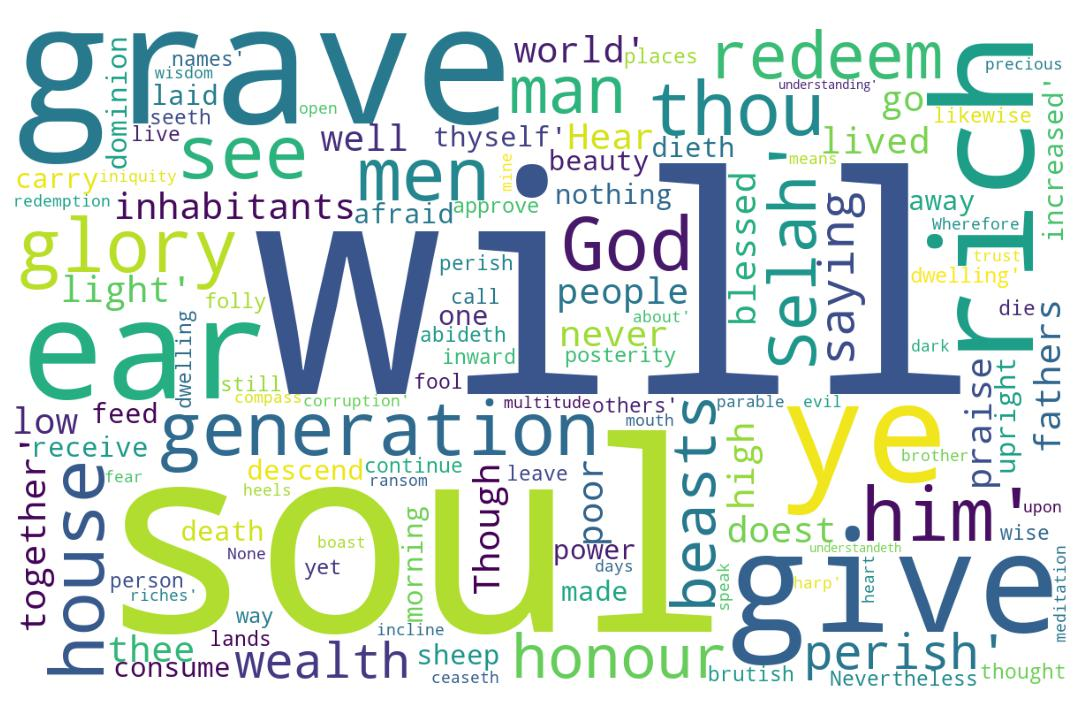
\includegraphics[width=\linewidth]{19OT-Psalms/Psalm49-WordCloud.jpg}
  \caption{Psalm 49 Word Cloud}
  \label{fig:Psalm 49 word Cloud}
\end{figure}

\marginpar{\scriptsize \centering \fcolorbox{bone}{lime}{\textbf{BIG PROBLEMS STILL REMAIN}}\\ (Psalm 49:1-20) \begin{compactenum}[I.][8]
    \item \textbf{Religious Conflict} \index[scripture]{Psalms!Psa 049:13} (Psa 49:13)
    \item \textbf{War} \index[scripture]{Psalms!Psa 049:13} (Psa 49:13)
    \item \textbf{Famine} \index[scripture]{Psalms!Psa 049:13} (Psa 49:13)
    \item \textbf{Sickness} \index[scripture]{Psalms!Psa 049:13} (Psa 49:13)
    \item \textbf{Death} \index[scripture]{Psalms!Psa 049:13} (Psa 49:13)
    \item \textbf{Natural Disasters} \index[scripture]{Psalms!Psa 049:13} (Psa 49:13)
    \item \textbf{Murder and Theft} \index[scripture]{Psalms!Psa 049:13} (Psa 49:13)
\end{compactenum}}
    
%%%%%%%%%%%%%%%%%%%%%%%%%%%%%%%%%%%%%
%%%%%%%%%%%%%%%%%%%%%%%%%%%%%%%%%%%%%
\footnote{\textcolor[cmyk]{0.99998,1,0,0}{\hyperlink{TOC}{Return to end of Table of Contents.}}}\footnote{\href{https://audiobible.com/bible/psalms_49.html}{\textcolor[cmyk]{0.99998,1,0,0}{Psalms Audio}}}\textcolor[cmyk]{0.99998,1,0,0}{To the chief Musician, A Psalm for the sons of Korah.}\footnote{This is one of the ``orphan'' psalm, with no known author (anonymous), But, it is one of eleven psalms that were for the sons of Korah. (Psalm 42, 44, 45, 46, 47, 48, 49, 84, 85, 87, and 88). The sons of Korah descended from a father who perished under the wrath and curse of God because of his arrogance and pride.   As Korah was a Levite, grandson of Kohath, great-grandson of Levi, this only aggravated his fault, and typifies the sin of Israel, keepers of the oracles of God. \cite{Phillips2001ExploringPsalms1} The count of the psalms for the sons of Korah points to the number 11 as the number of the ``remnant'' as does Hebrews 11 which lists those distinct and select people know for the exercise of faith.}\\
\\
\textcolor[cmyk]{0.99998,1,0,0}{Hear this, all \emph{ye} people; give ear, all \emph{ye} inhabitants of the world:}
[2] \textcolor[cmyk]{0.99998,1,0,0}{Both low and high, rich and poor, together.}
[3] \textcolor[cmyk]{0.99998,1,0,0}{My mouth shall speak of wisdom; and the meditation of my heart \emph{shall} \emph{be} of \fcolorbox{bone}{MYGOLD}{understanding}.}
[4] \textcolor[cmyk]{0.99998,1,0,0}{I will incline mine ear to a parable: I will open my dark saying upon the harp.}
[5] \textcolor[cmyk]{0.99998,1,0,0}{Wherefore should I fear in the days of evil, \emph{when} the iniquity of my heels shall compass me about?}\footnote{The words ``heels'' is found four times in scripture, signifying that someone’s iniquities are following them. What we have done catches up with us (vs. 5). The steps we have stepped, out run us eventually because we step slower and slower. Sooner or later they compass us round about: \cite{Ruckman1992Psalms}
\begin{compactenum}
\item \textbf{Genesis 49:17} -- Dan shall be a serpent by the way, an adder in the path, that biteth the horse heels, so that his rider shall fall backward.
\item \textbf{Job 13:27} -- Thou puttest my feet also in the stocks, and lookest narrowly unto all my paths; thou settest a print upon the heels of my feet.
\item \textbf{Psalm 49:5} -- Wherefore should I fear in the days of evil, \emph{when} the iniquity of my heels shall compass me about?
\item \textbf{Jeremiah 13:22} -- And if thou say in thine heart, Wherefore come these things upon me? For the greatness of thine iniquity are thy skirts discovered, \emph{and} thy heels made bare.
\end{compactenum} }
[6] \textcolor[cmyk]{0.99998,1,0,0}{They that trust in \fcolorbox{bone}{bone}{their} wealth, and boast themselves in the multitude of \fcolorbox{bone}{bone}{their} riches;}\marginpar{\scriptsize \textcolor[rgb]{0.00,0.545,0.269}{$\rightarrow$``Their'' things: 
\begin{compactenum}
	\item their wealth [6, 10],
	\item their riches [6],
	\item their soul [7],
	\item their inward thought [11],
	\item their houses [11],
	\item their dwelling places [11],
	\item their lands [11],
	\item their names [11],
	\item their way [13],
	\item their folly [13],
	\item their posterity [13],
	\item their sayings [13],
	\item their beauty [15], and
	\item dwelling  [15].
\end{compactenum}}}
[7] \textcolor[cmyk]{0.99998,1,0,0}{None \emph{of} \emph{them} can by any means redeem his brother, nor give to God a ransom for him:}
[8] \textcolor[cmyk]{0.99998,1,0,0}{(For the redemption of \fcolorbox{bone}{bone}{their} soul \emph{is} precious, and it ceaseth for ever:)}
[9] \textcolor[cmyk]{0.99998,1,0,0}{That he should still live for ever, \emph{and} not see corruption.}
[10] \textcolor[cmyk]{0.99998,1,0,0}{For he seeth \emph{that} wise men die, likewise the fool and the brutish person perish, and leave \fcolorbox{bone}{bone}{their} wealth to others.}
[11] \textcolor[cmyk]{0.99998,1,0,0}{Their inward thought \emph{is}, \emph{that} \fcolorbox{bone}{bone}{their} houses \emph{shall} \emph{continue} for ever, \emph{and} \fcolorbox{bone}{bone}{their} dwelling places to all generations; they call \emph{their} lands after \fcolorbox{bone}{bone}{their} own names.}
[12] \textcolor[cmyk]{0.99998,1,0,0}{Nevertheless man \emph{being} in honour abideth not: he is like the beasts \emph{that} perish.}
[13] \textcolor[cmyk]{0.99998,1,0,0}{This \fcolorbox{bone}{lime}{\fcolorbox{bone}{bone}{their} way} \emph{is} \fcolorbox{bone}{bone}{their} folly: yet \fcolorbox{bone}{bone}{their} posterity approve \fcolorbox{bone}{bone}{their} sayings. Selah.}
[14] \textcolor[cmyk]{0.99998,1,0,0}{Like sheep they are laid in the grave; death shall feed on them; and the upright shall have dominion over them in the morning; and \fcolorbox{bone}{bone}{their} beauty shall consume in the grave from \fcolorbox{bone}{bone}{their} dwelling.}
[15] \textcolor[cmyk]{0.99998,1,0,0}{But God will redeem my soul from the power of the grave: for he shall receive me. Selah.}
[16] \textcolor[cmyk]{0.99998,1,0,0}{Be not thou afraid when one is made rich, when the glory of his house is increased;}
[17] \textcolor[cmyk]{0.99998,1,0,0}{For when he dieth he shall carry nothing away: his glory shall not descend after him.}
[18] \textcolor[cmyk]{0.99998,1,0,0}{Though while he lived he blessed his soul: and \emph{men} will praise thee, when thou doest well to thyself.}
[19] \textcolor[cmyk]{0.99998,1,0,0}{He shall go to the generation of his fathers; they shall never see light.}
[20] \textcolor[cmyk]{0.99998,1,0,0}{Man \emph{that} \emph{is} in honour, and \fcolorbox{bone}{MYGOLD}{understandeth} not, is like the beasts \emph{that} perish.}
\index[NWIV]{13!Psalms!Psa 49:1}\index[AWIP]{Hear!Psalms!Psa 49:1}\index[AWIP]{this!Psalms!Psa 49:1}\index[AWIP]{all!Psalms!Psa 49:1}\index[AWIP]{all!Psalms!Psa 49:1 (2)}\index[AWIP]{\emph{ye}!Psalms!Psa 49:1}\index[AWIP]{\emph{ye}!Psalms!Psa 49:1 (2)}\index[AWIP]{people!Psalms!Psa 49:1}\index[AWIP]{give!Psalms!Psa 49:1}\index[AWIP]{ear!Psalms!Psa 49:1}\index[AWIP]{inhabitants!Psalms!Psa 49:1}\index[AWIP]{of!Psalms!Psa 49:1}\index[AWIP]{the!Psalms!Psa 49:1}\index[AWIP]{world!Psalms!Psa 49:1}\index[AWIP]{\emph{ye}!Psalms!Psa 49:1}\index[AWIP]{\emph{ye}!Psalms!Psa 49:1 (2)}

\index[NWIV]{8!Psalms!Psa 49:2}\index[AWIP]{Both!Psalms!Psa 49:2}\index[AWIP]{low!Psalms!Psa 49:2}\index[AWIP]{and!Psalms!Psa 49:2}\index[AWIP]{and!Psalms!Psa 49:2 (2)}\index[AWIP]{high!Psalms!Psa 49:2}\index[AWIP]{rich!Psalms!Psa 49:2}\index[AWIP]{poor!Psalms!Psa 49:2}\index[AWIP]{together!Psalms!Psa 49:2}

\index[NWIV]{16!Psalms!Psa 49:3}\index[AWIP]{My!Psalms!Psa 49:3}\index[AWIP]{mouth!Psalms!Psa 49:3}\index[AWIP]{shall!Psalms!Psa 49:3}\index[AWIP]{speak!Psalms!Psa 49:3}\index[AWIP]{of!Psalms!Psa 49:3}\index[AWIP]{of!Psalms!Psa 49:3 (2)}\index[AWIP]{of!Psalms!Psa 49:3 (3)}\index[AWIP]{wisdom!Psalms!Psa 49:3}\index[AWIP]{and!Psalms!Psa 49:3}\index[AWIP]{the!Psalms!Psa 49:3}\index[AWIP]{meditation!Psalms!Psa 49:3}\index[AWIP]{my!Psalms!Psa 49:3}\index[AWIP]{heart!Psalms!Psa 49:3}\index[AWIP]{\emph{shall}!Psalms!Psa 49:3}\index[AWIP]{\emph{be}!Psalms!Psa 49:3}\index[AWIP]{understanding!Psalms!Psa 49:3}\index[AWIP]{\emph{shall}!Psalms!Psa 49:3}\index[AWIP]{\emph{be}!Psalms!Psa 49:3}

\index[NWIV]{17!Psalms!Psa 49:4}\index[AWIP]{I!Psalms!Psa 49:4}\index[AWIP]{I!Psalms!Psa 49:4 (2)}\index[AWIP]{will!Psalms!Psa 49:4}\index[AWIP]{will!Psalms!Psa 49:4 (2)}\index[AWIP]{incline!Psalms!Psa 49:4}\index[AWIP]{mine!Psalms!Psa 49:4}\index[AWIP]{ear!Psalms!Psa 49:4}\index[AWIP]{to!Psalms!Psa 49:4}\index[AWIP]{a!Psalms!Psa 49:4}\index[AWIP]{parable!Psalms!Psa 49:4}\index[AWIP]{open!Psalms!Psa 49:4}\index[AWIP]{my!Psalms!Psa 49:4}\index[AWIP]{dark!Psalms!Psa 49:4}\index[AWIP]{saying!Psalms!Psa 49:4}\index[AWIP]{upon!Psalms!Psa 49:4}\index[AWIP]{the!Psalms!Psa 49:4}\index[AWIP]{harp!Psalms!Psa 49:4}

\index[NWIV]{19!Psalms!Psa 49:5}\index[AWIP]{Wherefore!Psalms!Psa 49:5}\index[AWIP]{should!Psalms!Psa 49:5}\index[AWIP]{I!Psalms!Psa 49:5}\index[AWIP]{fear!Psalms!Psa 49:5}\index[AWIP]{in!Psalms!Psa 49:5}\index[AWIP]{the!Psalms!Psa 49:5}\index[AWIP]{the!Psalms!Psa 49:5 (2)}\index[AWIP]{days!Psalms!Psa 49:5}\index[AWIP]{of!Psalms!Psa 49:5}\index[AWIP]{of!Psalms!Psa 49:5 (2)}\index[AWIP]{evil!Psalms!Psa 49:5}\index[AWIP]{\emph{when}!Psalms!Psa 49:5}\index[AWIP]{iniquity!Psalms!Psa 49:5}\index[AWIP]{my!Psalms!Psa 49:5}\index[AWIP]{heels!Psalms!Psa 49:5}\index[AWIP]{shall!Psalms!Psa 49:5}\index[AWIP]{compass!Psalms!Psa 49:5}\index[AWIP]{me!Psalms!Psa 49:5}\index[AWIP]{about?!Psalms!Psa 49:5}\index[AWIP]{\emph{when}!Psalms!Psa 49:5}

\index[NWIV]{15!Psalms!Psa 49:6}\index[AWIP]{They!Psalms!Psa 49:6}\index[AWIP]{that!Psalms!Psa 49:6}\index[AWIP]{trust!Psalms!Psa 49:6}\index[AWIP]{in!Psalms!Psa 49:6}\index[AWIP]{in!Psalms!Psa 49:6 (2)}\index[AWIP]{their!Psalms!Psa 49:6}\index[AWIP]{their!Psalms!Psa 49:6 (2)}\index[AWIP]{wealth!Psalms!Psa 49:6}\index[AWIP]{and!Psalms!Psa 49:6}\index[AWIP]{boast!Psalms!Psa 49:6}\index[AWIP]{themselves!Psalms!Psa 49:6}\index[AWIP]{the!Psalms!Psa 49:6}\index[AWIP]{multitude!Psalms!Psa 49:6}\index[AWIP]{of!Psalms!Psa 49:6}\index[AWIP]{riches!Psalms!Psa 49:6}

\index[NWIV]{18!Psalms!Psa 49:7}\index[AWIP]{None!Psalms!Psa 49:7}\index[AWIP]{\emph{of}!Psalms!Psa 49:7}\index[AWIP]{\emph{them}!Psalms!Psa 49:7}\index[AWIP]{can!Psalms!Psa 49:7}\index[AWIP]{by!Psalms!Psa 49:7}\index[AWIP]{any!Psalms!Psa 49:7}\index[AWIP]{means!Psalms!Psa 49:7}\index[AWIP]{redeem!Psalms!Psa 49:7}\index[AWIP]{his!Psalms!Psa 49:7}\index[AWIP]{brother!Psalms!Psa 49:7}\index[AWIP]{nor!Psalms!Psa 49:7}\index[AWIP]{give!Psalms!Psa 49:7}\index[AWIP]{to!Psalms!Psa 49:7}\index[AWIP]{God!Psalms!Psa 49:7}\index[AWIP]{a!Psalms!Psa 49:7}\index[AWIP]{ransom!Psalms!Psa 49:7}\index[AWIP]{for!Psalms!Psa 49:7}\index[AWIP]{him!Psalms!Psa 49:7}\index[AWIP]{\emph{of}!Psalms!Psa 49:7}\index[AWIP]{\emph{them}!Psalms!Psa 49:7}

\index[NWIV]{13!Psalms!Psa 49:8}\index[AWIP]{(For!Psalms!Psa 49:8}\index[AWIP]{the!Psalms!Psa 49:8}\index[AWIP]{redemption!Psalms!Psa 49:8}\index[AWIP]{of!Psalms!Psa 49:8}\index[AWIP]{their!Psalms!Psa 49:8}\index[AWIP]{soul!Psalms!Psa 49:8}\index[AWIP]{\emph{is}!Psalms!Psa 49:8}\index[AWIP]{precious!Psalms!Psa 49:8}\index[AWIP]{and!Psalms!Psa 49:8}\index[AWIP]{it!Psalms!Psa 49:8}\index[AWIP]{ceaseth!Psalms!Psa 49:8}\index[AWIP]{for!Psalms!Psa 49:8}\index[AWIP]{ever)!Psalms!Psa 49:8}\index[AWIP]{\emph{is}!Psalms!Psa 49:8}

\index[NWIV]{11!Psalms!Psa 49:9}\index[AWIP]{That!Psalms!Psa 49:9}\index[AWIP]{he!Psalms!Psa 49:9}\index[AWIP]{should!Psalms!Psa 49:9}\index[AWIP]{still!Psalms!Psa 49:9}\index[AWIP]{live!Psalms!Psa 49:9}\index[AWIP]{for!Psalms!Psa 49:9}\index[AWIP]{ever!Psalms!Psa 49:9}\index[AWIP]{\emph{and}!Psalms!Psa 49:9}\index[AWIP]{not!Psalms!Psa 49:9}\index[AWIP]{see!Psalms!Psa 49:9}\index[AWIP]{corruption!Psalms!Psa 49:9}\index[AWIP]{\emph{and}!Psalms!Psa 49:9}

\index[NWIV]{21!Psalms!Psa 49:10}\index[AWIP]{For!Psalms!Psa 49:10}\index[AWIP]{he!Psalms!Psa 49:10}\index[AWIP]{seeth!Psalms!Psa 49:10}\index[AWIP]{\emph{that}!Psalms!Psa 49:10}\index[AWIP]{wise!Psalms!Psa 49:10}\index[AWIP]{men!Psalms!Psa 49:10}\index[AWIP]{die!Psalms!Psa 49:10}\index[AWIP]{likewise!Psalms!Psa 49:10}\index[AWIP]{the!Psalms!Psa 49:10}\index[AWIP]{the!Psalms!Psa 49:10 (2)}\index[AWIP]{fool!Psalms!Psa 49:10}\index[AWIP]{and!Psalms!Psa 49:10}\index[AWIP]{and!Psalms!Psa 49:10 (2)}\index[AWIP]{brutish!Psalms!Psa 49:10}\index[AWIP]{person!Psalms!Psa 49:10}\index[AWIP]{perish!Psalms!Psa 49:10}\index[AWIP]{leave!Psalms!Psa 49:10}\index[AWIP]{their!Psalms!Psa 49:10}\index[AWIP]{wealth!Psalms!Psa 49:10}\index[AWIP]{to!Psalms!Psa 49:10}\index[AWIP]{others!Psalms!Psa 49:10}\index[AWIP]{\emph{that}!Psalms!Psa 49:10}

\index[NWIV]{26!Psalms!Psa 49:11}\index[AWIP]{Their!Psalms!Psa 49:11}\index[AWIP]{inward!Psalms!Psa 49:11}\index[AWIP]{thought!Psalms!Psa 49:11}\index[AWIP]{\emph{is}!Psalms!Psa 49:11}\index[AWIP]{\emph{that}!Psalms!Psa 49:11}\index[AWIP]{their!Psalms!Psa 49:11}\index[AWIP]{their!Psalms!Psa 49:11 (2)}\index[AWIP]{their!Psalms!Psa 49:11 (3)}\index[AWIP]{houses!Psalms!Psa 49:11}\index[AWIP]{\emph{shall}!Psalms!Psa 49:11}\index[AWIP]{\emph{continue}!Psalms!Psa 49:11}\index[AWIP]{for!Psalms!Psa 49:11}\index[AWIP]{ever!Psalms!Psa 49:11}\index[AWIP]{\emph{and}!Psalms!Psa 49:11}\index[AWIP]{dwelling!Psalms!Psa 49:11}\index[AWIP]{places!Psalms!Psa 49:11}\index[AWIP]{to!Psalms!Psa 49:11}\index[AWIP]{all!Psalms!Psa 49:11}\index[AWIP]{generations!Psalms!Psa 49:11}\index[AWIP]{they!Psalms!Psa 49:11}\index[AWIP]{call!Psalms!Psa 49:11}\index[AWIP]{\emph{their}!Psalms!Psa 49:11}\index[AWIP]{lands!Psalms!Psa 49:11}\index[AWIP]{after!Psalms!Psa 49:11}\index[AWIP]{own!Psalms!Psa 49:11}\index[AWIP]{names!Psalms!Psa 49:11}\index[AWIP]{\emph{is}!Psalms!Psa 49:11}\index[AWIP]{\emph{that}!Psalms!Psa 49:11}\index[AWIP]{\emph{shall}!Psalms!Psa 49:11}\index[AWIP]{\emph{continue}!Psalms!Psa 49:11}\index[AWIP]{\emph{and}!Psalms!Psa 49:11}\index[AWIP]{\emph{their}!Psalms!Psa 49:11}

\index[NWIV]{14!Psalms!Psa 49:12}\index[AWIP]{Nevertheless!Psalms!Psa 49:12}\index[AWIP]{man!Psalms!Psa 49:12}\index[AWIP]{\emph{being}!Psalms!Psa 49:12}\index[AWIP]{in!Psalms!Psa 49:12}\index[AWIP]{honour!Psalms!Psa 49:12}\index[AWIP]{abideth!Psalms!Psa 49:12}\index[AWIP]{not!Psalms!Psa 49:12}\index[AWIP]{he!Psalms!Psa 49:12}\index[AWIP]{is!Psalms!Psa 49:12}\index[AWIP]{like!Psalms!Psa 49:12}\index[AWIP]{the!Psalms!Psa 49:12}\index[AWIP]{beasts!Psalms!Psa 49:12}\index[AWIP]{\emph{that}!Psalms!Psa 49:12}\index[AWIP]{perish!Psalms!Psa 49:12}\index[AWIP]{\emph{being}!Psalms!Psa 49:12}\index[AWIP]{\emph{that}!Psalms!Psa 49:12}

\index[NWIV]{13!Psalms!Psa 49:13}\index[AWIP]{This!Psalms!Psa 49:13}\index[AWIP]{their!Psalms!Psa 49:13}\index[AWIP]{their!Psalms!Psa 49:13 (2)}\index[AWIP]{their!Psalms!Psa 49:13 (3)}\index[AWIP]{their!Psalms!Psa 49:13 (4)}\index[AWIP]{way!Psalms!Psa 49:13}\index[AWIP]{\emph{is}!Psalms!Psa 49:13}\index[AWIP]{folly!Psalms!Psa 49:13}\index[AWIP]{yet!Psalms!Psa 49:13}\index[AWIP]{posterity!Psalms!Psa 49:13}\index[AWIP]{approve!Psalms!Psa 49:13}\index[AWIP]{sayings!Psalms!Psa 49:13}\index[AWIP]{Selah!Psalms!Psa 49:13}\index[AWIP]{\emph{is}!Psalms!Psa 49:13}

\index[NWIV]{35!Psalms!Psa 49:14}\index[AWIP]{Like!Psalms!Psa 49:14}\index[AWIP]{sheep!Psalms!Psa 49:14}\index[AWIP]{they!Psalms!Psa 49:14}\index[AWIP]{are!Psalms!Psa 49:14}\index[AWIP]{laid!Psalms!Psa 49:14}\index[AWIP]{in!Psalms!Psa 49:14}\index[AWIP]{in!Psalms!Psa 49:14 (2)}\index[AWIP]{in!Psalms!Psa 49:14 (3)}\index[AWIP]{the!Psalms!Psa 49:14}\index[AWIP]{the!Psalms!Psa 49:14 (2)}\index[AWIP]{the!Psalms!Psa 49:14 (3)}\index[AWIP]{the!Psalms!Psa 49:14 (4)}\index[AWIP]{grave!Psalms!Psa 49:14}\index[AWIP]{grave!Psalms!Psa 49:14 (2)}\index[AWIP]{death!Psalms!Psa 49:14}\index[AWIP]{shall!Psalms!Psa 49:14}\index[AWIP]{shall!Psalms!Psa 49:14 (2)}\index[AWIP]{shall!Psalms!Psa 49:14 (3)}\index[AWIP]{feed!Psalms!Psa 49:14}\index[AWIP]{on!Psalms!Psa 49:14}\index[AWIP]{them!Psalms!Psa 49:14}\index[AWIP]{them!Psalms!Psa 49:14 (2)}\index[AWIP]{and!Psalms!Psa 49:14}\index[AWIP]{and!Psalms!Psa 49:14 (2)}\index[AWIP]{upright!Psalms!Psa 49:14}\index[AWIP]{have!Psalms!Psa 49:14}\index[AWIP]{dominion!Psalms!Psa 49:14}\index[AWIP]{over!Psalms!Psa 49:14}\index[AWIP]{morning!Psalms!Psa 49:14}\index[AWIP]{their!Psalms!Psa 49:14}\index[AWIP]{their!Psalms!Psa 49:14 (2)}\index[AWIP]{beauty!Psalms!Psa 49:14}\index[AWIP]{consume!Psalms!Psa 49:14}\index[AWIP]{from!Psalms!Psa 49:14}\index[AWIP]{dwelling!Psalms!Psa 49:14}

\index[NWIV]{18!Psalms!Psa 49:15}\index[AWIP]{But!Psalms!Psa 49:15}\index[AWIP]{God!Psalms!Psa 49:15}\index[AWIP]{will!Psalms!Psa 49:15}\index[AWIP]{redeem!Psalms!Psa 49:15}\index[AWIP]{my!Psalms!Psa 49:15}\index[AWIP]{soul!Psalms!Psa 49:15}\index[AWIP]{from!Psalms!Psa 49:15}\index[AWIP]{the!Psalms!Psa 49:15}\index[AWIP]{the!Psalms!Psa 49:15 (2)}\index[AWIP]{power!Psalms!Psa 49:15}\index[AWIP]{of!Psalms!Psa 49:15}\index[AWIP]{grave!Psalms!Psa 49:15}\index[AWIP]{for!Psalms!Psa 49:15}\index[AWIP]{he!Psalms!Psa 49:15}\index[AWIP]{shall!Psalms!Psa 49:15}\index[AWIP]{receive!Psalms!Psa 49:15}\index[AWIP]{me!Psalms!Psa 49:15}\index[AWIP]{Selah!Psalms!Psa 49:15}

\index[NWIV]{17!Psalms!Psa 49:16}\index[AWIP]{Be!Psalms!Psa 49:16}\index[AWIP]{not!Psalms!Psa 49:16}\index[AWIP]{thou!Psalms!Psa 49:16}\index[AWIP]{afraid!Psalms!Psa 49:16}\index[AWIP]{when!Psalms!Psa 49:16}\index[AWIP]{when!Psalms!Psa 49:16 (2)}\index[AWIP]{one!Psalms!Psa 49:16}\index[AWIP]{is!Psalms!Psa 49:16}\index[AWIP]{is!Psalms!Psa 49:16 (2)}\index[AWIP]{made!Psalms!Psa 49:16}\index[AWIP]{rich!Psalms!Psa 49:16}\index[AWIP]{the!Psalms!Psa 49:16}\index[AWIP]{glory!Psalms!Psa 49:16}\index[AWIP]{of!Psalms!Psa 49:16}\index[AWIP]{his!Psalms!Psa 49:16}\index[AWIP]{house!Psalms!Psa 49:16}\index[AWIP]{increased!Psalms!Psa 49:16}

\index[NWIV]{16!Psalms!Psa 49:17}\index[AWIP]{For!Psalms!Psa 49:17}\index[AWIP]{when!Psalms!Psa 49:17}\index[AWIP]{he!Psalms!Psa 49:17}\index[AWIP]{he!Psalms!Psa 49:17 (2)}\index[AWIP]{dieth!Psalms!Psa 49:17}\index[AWIP]{shall!Psalms!Psa 49:17}\index[AWIP]{shall!Psalms!Psa 49:17 (2)}\index[AWIP]{carry!Psalms!Psa 49:17}\index[AWIP]{nothing!Psalms!Psa 49:17}\index[AWIP]{away!Psalms!Psa 49:17}\index[AWIP]{his!Psalms!Psa 49:17}\index[AWIP]{glory!Psalms!Psa 49:17}\index[AWIP]{not!Psalms!Psa 49:17}\index[AWIP]{descend!Psalms!Psa 49:17}\index[AWIP]{after!Psalms!Psa 49:17}\index[AWIP]{him!Psalms!Psa 49:17}

\index[NWIV]{19!Psalms!Psa 49:18}\index[AWIP]{Though!Psalms!Psa 49:18}\index[AWIP]{while!Psalms!Psa 49:18}\index[AWIP]{he!Psalms!Psa 49:18}\index[AWIP]{he!Psalms!Psa 49:18 (2)}\index[AWIP]{lived!Psalms!Psa 49:18}\index[AWIP]{blessed!Psalms!Psa 49:18}\index[AWIP]{his!Psalms!Psa 49:18}\index[AWIP]{soul!Psalms!Psa 49:18}\index[AWIP]{and!Psalms!Psa 49:18}\index[AWIP]{\emph{men}!Psalms!Psa 49:18}\index[AWIP]{will!Psalms!Psa 49:18}\index[AWIP]{praise!Psalms!Psa 49:18}\index[AWIP]{thee!Psalms!Psa 49:18}\index[AWIP]{when!Psalms!Psa 49:18}\index[AWIP]{thou!Psalms!Psa 49:18}\index[AWIP]{doest!Psalms!Psa 49:18}\index[AWIP]{well!Psalms!Psa 49:18}\index[AWIP]{to!Psalms!Psa 49:18}\index[AWIP]{thyself!Psalms!Psa 49:18}\index[AWIP]{\emph{men}!Psalms!Psa 49:18}

\index[NWIV]{14!Psalms!Psa 49:19}\index[AWIP]{He!Psalms!Psa 49:19}\index[AWIP]{shall!Psalms!Psa 49:19}\index[AWIP]{shall!Psalms!Psa 49:19 (2)}\index[AWIP]{go!Psalms!Psa 49:19}\index[AWIP]{to!Psalms!Psa 49:19}\index[AWIP]{the!Psalms!Psa 49:19}\index[AWIP]{generation!Psalms!Psa 49:19}\index[AWIP]{of!Psalms!Psa 49:19}\index[AWIP]{his!Psalms!Psa 49:19}\index[AWIP]{fathers!Psalms!Psa 49:19}\index[AWIP]{they!Psalms!Psa 49:19}\index[AWIP]{never!Psalms!Psa 49:19}\index[AWIP]{see!Psalms!Psa 49:19}\index[AWIP]{light!Psalms!Psa 49:19}

\index[NWIV]{14!Psalms!Psa 49:20}\index[AWIP]{Man!Psalms!Psa 49:20}\index[AWIP]{\emph{that}!Psalms!Psa 49:20}\index[AWIP]{\emph{that}!Psalms!Psa 49:20 (2)}\index[AWIP]{\emph{is}!Psalms!Psa 49:20}\index[AWIP]{in!Psalms!Psa 49:20}\index[AWIP]{honour!Psalms!Psa 49:20}\index[AWIP]{and!Psalms!Psa 49:20}\index[AWIP]{understandeth!Psalms!Psa 49:20}\index[AWIP]{not!Psalms!Psa 49:20}\index[AWIP]{is!Psalms!Psa 49:20}\index[AWIP]{like!Psalms!Psa 49:20}\index[AWIP]{the!Psalms!Psa 49:20}\index[AWIP]{beasts!Psalms!Psa 49:20}\index[AWIP]{perish!Psalms!Psa 49:20}\index[AWIP]{\emph{that}!Psalms!Psa 49:20}\index[AWIP]{\emph{that}!Psalms!Psa 49:20 (2)}\index[AWIP]{\emph{is}!Psalms!Psa 49:20}


\section{Psalm 49 Outlines}

\subsection{My Outlines}

\subsubsection{The Big Problems Still Remain}
\textbf{Introduction:} Psalm 49 has three verses with 13 words (1, 8, and 13), showing that the word will rebel against truth and choose to believe (in vain) that mankind can solve his basic problems, But he has not and will not. Another title could be ``New Year -- Same Unsolved Problems'':
\index[speaker]{Keith Anthony!Psalm 049 (The Reigning King)}
\index[series]{Psalms (Keith Anthony)!Psalm 049  (The Reigning King) }
\index[date]{2016/07/25!Psalm 049 (The Reigning King) (Keith Anthony)}
\begin{compactenum}[I.][8]
    \item \textbf{Religious Conflict} \index[scripture]{Psalms!Psa 049:13} (Psa 49:13)
    \item \textbf{War} \index[scripture]{Psalms!Psa 049:13} (Psa 49:13)
    \item \textbf{Famine} \index[scripture]{Psalms!Psa 049:13} (Psa 49:13)
    \item \textbf{Sickness} \index[scripture]{Psalms!Psa 049:13} (Psa 49:13)
    \item \textbf{Death} \index[scripture]{Psalms!Psa 049:13} (Psa 49:13)
    \item \textbf{Natural Disasters} \index[scripture]{Psalms!Psa 049:13} (Psa 49:13)
    \item \textbf{Murder and Theft} \index[scripture]{Psalms!Psa 049:13} (Psa 49:13)
\end{compactenum}


\subsubsection{The Big Problems Still Remain}
%\textbf{Introduction:} Psalm 49 has three verses with 13 words (1, 8, and 13), showing that the word will rebel against truth and choose to believe (in vain) that mankind can solve his basic problems, But he has not and will not. Another title could be ``New Year -- Same Unsolved Problems'':
\index[speaker]{Keith Anthony!Psalm 049 (The Beasts that Perish)}
\index[series]{Psalms (Keith Anthony)!Psalm 049  (The Beasts that Perish) }
\index[date]{2022/02/18!Psalm 049 (\textbf{The Reigning King}The Beasts that Perish) (Keith Anthony)}

\begin{compactenum}[I.][8]
    \item The \textbf{Basic Problems}
    \item The \textbf{Brutish People}
    \item The \textbf{Broken ``Progress''}
    \item The \textbf{Bestowed Possessions}
    \item The \textbf{Beauty that Passes}
    \item The \textbf{Beasts that Perish}
\end{compactenum}


\subsection{Outlines from Others}

\section{Psalm 49 Comments}

\subsection{Numeric Nuggets}
Verses 1, 8, and 13 have 13 words. Verses 6,  8, 19, and 20 have thirteen unique words. The word ``their'' is used thirteen time in the psalm. (``Their'' is used once, and ``\emph{their}'' is used once.) The 13-letter words ``understanding'' and ``understandeth'' are found in the chapter.

\subsection{Psalm 49:4}
The phrase ``dark saying'', then, is associated with parables. This is the only instance of the phrase, and the phrase ``dark sayings'' is found only twice: \begin{compactenum}
\item \textbf{Psalm 78:2} -- I will open my mouth in a parable: I will utter dark sayings of old: 
\item \textbf{Proverbs 1:6} -- To understand a proverb, and the interpretation; the words of the wise, and their dark sayings.
\end{compactenum}
It is a truth that the ear must be inclined to God to understand a parable before it can be played and sung on a harp. That is why the Psalm was called a ``parable.'' It contains a great deal more than simply warnings against living and dying without redemption or a right relationship to God. The Psalmist is an endtime Jew, when the iniquity of Israel is being paid off double (Isaiah 40:2) for his sin of rejecting the Messiah. The full payment is described in the Lamentations, and the full payment will make Hitler’s holocaust look like exactly what it was: a rehearsal (see Jeremiah 16:16, Amos 9:2). This is a saved Jew who is saying, “Wherefore should I fear in the days of evil,” because he knows how the days of evil are going to end (Matthew 24:30, Luke 21:28). Once again the “man” (verses 12, 16, 17, and 19) is a MAN (the Antichrist, see Psalm 52), and “MAN” in the aggregate. This is the forty-ninth Psalm: seven times seven, the completion of Gentile revelation.\cite{Ruckman1992Psalms}

\subsection{Psalm 49:13}
The sayings of the degenerate ``big shots'' are legend. It takes volumes to record them. They are chaff in the wind. No group of religious leaders, political leaders, educators, scientists, humanitarians, dictators, philosophers, doctors, lawyers, judges, and millionaires combined (through a period of six millenniums) could solve one major problem of mankind. There are seven:\cite{Ruckman1992Psalms}\begin{compactenum}
    \item Religious disunity.
    \item Wars between nations.
    \item Famine and starvation.
    \item Sickness.
    \item Death.
    \item Earthquakes and hurricanes.
    \item Murder and theft.
\end{compactenum}

\subsection{Psalm 49:20}
The verse makes a comparison between what God honors and what mankind honors. \cite{Ruckman1992Psalms} \begin{compactenum}
    \item Unsaved women  are called “pigs” in scripture (2 Pet. 2:22; Prov. 11:22).
    \item Unsaved men are called “dogs” (Rev. 22:15; 2 Pet. 2:22).
    \item Unsaved religious leaders are called “vipers” (Matt. 23:33).
\end{compactenum}
Psalm 49 is a self-explanatory repeat of the refrain so familiar to the reader of the Book of Ecclesiastes. \cite{Ruckman1992Psalms}\begin{compactenum}
\item You came in naked, and you go out naked (vs. 17). See  1 Timothy 6:7 and Job 1:21.
\item You can make yourself happy by “realizing” or “finding’’ yourself (vs. 18), and if you make your “bundle” before the funeral, men will praise you (vs. 18): mainly to get your money.
\item You go the way of all your flesh (vs. 19), and if they are lost like you are -— the rich man had five brothers (Luke 16:28) -— they too will die like dogs (vs. 20). You do not come up at the end of the Tribulation (vs. 14) to enter the Millennium; you stay down one thousand years, and then come up to the White Throne Judgment (Rev. 20).
\end{compactenum}
\subsection{Psalm 49 Repeated Phrases}


%%%%%%%%%%
%%%%%%%%%%
\normalsize
 
\begin{center}
\begin{longtable}{|c|c|}
\caption[Psalm 49 Repeated Phrases]{Psalm 49 Repeated Phrases}\label{table:Repeated Phrases Psalm4 9} \\
\hline \multicolumn{1}{|c|}{\textbf{Phrase}} & \multicolumn{1}{c|}{\textbf{Frequency}} \\ \hline 
\endfirsthead
 
\multicolumn{2}{c}
{{\bfseries \tablename\ \thetable{} -- continued from previous page}} \\  
\hline \multicolumn{1}{|c|}{\textbf{Phrase}} & \multicolumn{1}{c|}{\textbf{Frequency}} \\ \hline 
\endhead
 
\hline \multicolumn{2}{c}{{ }} \\ \hline
\endfoot 
in the & 5\\ \hline 
and the & 3\\ \hline 
the grave & 3\\ \hline 
\end{longtable}
\end{center}



%%%%%%%%%%
%%%%%%%%%%



\section{Psalm 49 Statistics}

%%%%%%%%%%%%%%%%%%%%%%%%%%%
%%%%% Word Statistics
%%%%%%%%%%%%%%%%%%%%%%%%%%


\normalsize



\subsection{Chapter Word Statistics}


%%%%%%%%%%
%%%%%%%%%%
 
\begin{center}
\begin{longtable}{l|c|c|c|c}
\caption[Stats for Psalm 49]{Stats for Psalm 49} \label{table:Stats for Psalm 49} \\ 
\hline \multicolumn{1}{|c|}{\textbf{Verse(s)}} & \multicolumn{1}{|c|}{\textbf{Count}} & \multicolumn{1}{|c|}{\textbf{Unique}} & \multicolumn{1}{|c|}{\textbf{Italics}} & \multicolumn{1}{|c|}{\textbf{Uniq Italic}}  \\ \hline 
\endfirsthead
 
\multicolumn{5}{c}
{{\bfseries \tablename\ \thetable{} -- continued from previous page}} \\  
\hline \multicolumn{1}{|c|}{\textbf{Verse(s)}} & \multicolumn{1}{|c|}{\textbf{Count}} & \multicolumn{1}{|c|}{\textbf{Unique}} & \multicolumn{1}{|c|}{\textbf{Italics}} & \multicolumn{1}{|c|}{\textbf{Uniq Italic}}  \\ \hline 
\endhead
 
\hline \multicolumn{5}{|r|}{{Continued if needed}} \\ \hline
\endfoot 
1 & 13 & 11 & 2 & 1\\ \hline
2 & 8 & 7 & 0 & 0\\ \hline
3 & 16 & 14 & 2 & 2\\ \hline
4 & 17 & 15 & 0 & 0\\ \hline
5 & 19 & 17 & 1 & 1\\ \hline
6 & 15 & 13 & 0 & 0\\ \hline
7 & 18 & 18 & 2 & 2\\ \hline
8 & 13 & 13 & 1 & 1\\ \hline
9 & 11 & 11 & 1 & 1\\ \hline
10 & 21 & 19 & 1 & 1\\ \hline
11 & 26 & 24 & 6 & 6\\ \hline
12 & 14 & 14 & 2 & 2\\ \hline
13 & 13 & 10 & 1 & 1\\ \hline
14 & 35 & 24 & 0 & 0\\ \hline
15 & 18 & 17 & 0 & 0\\ \hline
16 & 17 & 15 & 0 & 0\\ \hline
17 & 16 & 14 & 0 & 0\\ \hline
18 & 19 & 18 & 1 & 1\\ \hline
19 & 14 & 13 & 0 & 0\\ \hline
20 & 14 & 13 & 3 & 2\\ \hline
\hline \hline
Total & 337 & 188 & 23 & 13



\end{longtable}
\end{center}

%%%%%%%%%%
%%%%%%%%%%
 
\subsection{Words by Frequency}

\begin{center}
\begin{longtable}{l|r}
\caption[Word Frequencies in Psalm 49]{Word Frequencies in Psalm 49} \label{table:WordsIn-Psalm-49} \\ 
\hline \multicolumn{1}{|c|}{\textbf{Word}} & \multicolumn{1}{c|}{\textbf{Frequency}} \\ \hline 
\endfirsthead
 
\multicolumn{2}{c}
{{\bfseries \tablename\ \thetable{} -- continued from previous page}} \\ 
\hline \multicolumn{1}{|c|}{\textbf{Word}} & \multicolumn{1}{c|}{\textbf{Frequency}} \\ \hline 
\endhead
 
\hline \multicolumn{2}{|r|}{{Continued if needed}} \\ \hline
\endfoot
 
\hline \hline
\endlastfoot
the & 19 \\ \hline
their & 13 \\ \hline
of & 11 \\ \hline
and & 11 \\ \hline
shall & 10 \\ \hline
in & 8 \\ \hline
he & 8 \\ \hline
to & 6 \\ \hline
his & 5 \\ \hline
for & 5 \\ \hline
not & 5 \\ \hline
\emph{that} & 5 \\ \hline
my & 4 \\ \hline
will & 4 \\ \hline
\emph{is} & 4 \\ \hline
is & 4 \\ \hline
when & 4 \\ \hline
all & 3 \\ \hline
I & 3 \\ \hline
For & 3 \\ \hline
soul & 3 \\ \hline
ever & 3 \\ \hline
perish & 3 \\ \hline
they & 3 \\ \hline
grave & 3 \\ \hline
\emph{ye} & 2 \\ \hline
give & 2 \\ \hline
ear & 2 \\ \hline
rich & 2 \\ \hline
\emph{shall} & 2 \\ \hline
a & 2 \\ \hline
should & 2 \\ \hline
me & 2 \\ \hline
wealth & 2 \\ \hline
redeem & 2 \\ \hline
God & 2 \\ \hline
him & 2 \\ \hline
\emph{and} & 2 \\ \hline
see & 2 \\ \hline
dwelling & 2 \\ \hline
after & 2 \\ \hline
honour & 2 \\ \hline
like & 2 \\ \hline
beasts & 2 \\ \hline
Selah & 2 \\ \hline
them & 2 \\ \hline
from & 2 \\ \hline
thou & 2 \\ \hline
glory & 2 \\ \hline
Hear & 1 \\ \hline
this & 1 \\ \hline
people & 1 \\ \hline
inhabitants & 1 \\ \hline
world & 1 \\ \hline
Both & 1 \\ \hline
low & 1 \\ \hline
high & 1 \\ \hline
poor & 1 \\ \hline
together & 1 \\ \hline
My & 1 \\ \hline
mouth & 1 \\ \hline
speak & 1 \\ \hline
wisdom & 1 \\ \hline
meditation & 1 \\ \hline
heart & 1 \\ \hline
\emph{be} & 1 \\ \hline
understanding & 1 \\ \hline
incline & 1 \\ \hline
mine & 1 \\ \hline
parable & 1 \\ \hline
open & 1 \\ \hline
dark & 1 \\ \hline
saying & 1 \\ \hline
upon & 1 \\ \hline
harp & 1 \\ \hline
Wherefore & 1 \\ \hline
fear & 1 \\ \hline
days & 1 \\ \hline
evil & 1 \\ \hline
\emph{when} & 1 \\ \hline
iniquity & 1 \\ \hline
heels & 1 \\ \hline
compass & 1 \\ \hline
about & 1 \\ \hline
They & 1 \\ \hline
that & 1 \\ \hline
trust & 1 \\ \hline
boast & 1 \\ \hline
themselves & 1 \\ \hline
multitude & 1 \\ \hline
riches & 1 \\ \hline
None & 1 \\ \hline
\emph{of} & 1 \\ \hline
\emph{them} & 1 \\ \hline
can & 1 \\ \hline
by & 1 \\ \hline
any & 1 \\ \hline
means & 1 \\ \hline
brother & 1 \\ \hline
nor & 1 \\ \hline
ransom & 1 \\ \hline
redemption & 1 \\ \hline
precious & 1 \\ \hline
it & 1 \\ \hline
ceaseth & 1 \\ \hline
That & 1 \\ \hline
still & 1 \\ \hline
live & 1 \\ \hline
corruption & 1 \\ \hline
seeth & 1 \\ \hline
wise & 1 \\ \hline
men & 1 \\ \hline
die & 1 \\ \hline
likewise & 1 \\ \hline
fool & 1 \\ \hline
brutish & 1 \\ \hline
person & 1 \\ \hline
leave & 1 \\ \hline
others & 1 \\ \hline
Their & 1 \\ \hline
inward & 1 \\ \hline
thought & 1 \\ \hline
houses & 1 \\ \hline
\emph{continue} & 1 \\ \hline
places & 1 \\ \hline
generations & 1 \\ \hline
call & 1 \\ \hline
\emph{their} & 1 \\ \hline
lands & 1 \\ \hline
own & 1 \\ \hline
names & 1 \\ \hline
Nevertheless & 1 \\ \hline
man & 1 \\ \hline
\emph{being} & 1 \\ \hline
abideth & 1 \\ \hline
This & 1 \\ \hline
way & 1 \\ \hline
folly & 1 \\ \hline
yet & 1 \\ \hline
posterity & 1 \\ \hline
approve & 1 \\ \hline
sayings & 1 \\ \hline
Like & 1 \\ \hline
sheep & 1 \\ \hline
are & 1 \\ \hline
laid & 1 \\ \hline
death & 1 \\ \hline
feed & 1 \\ \hline
on & 1 \\ \hline
upright & 1 \\ \hline
have & 1 \\ \hline
dominion & 1 \\ \hline
over & 1 \\ \hline
morning & 1 \\ \hline
beauty & 1 \\ \hline
consume & 1 \\ \hline
But & 1 \\ \hline
power & 1 \\ \hline
receive & 1 \\ \hline
Be & 1 \\ \hline
afraid & 1 \\ \hline
one & 1 \\ \hline
made & 1 \\ \hline
house & 1 \\ \hline
increased & 1 \\ \hline
dieth & 1 \\ \hline
carry & 1 \\ \hline
nothing & 1 \\ \hline
away & 1 \\ \hline
descend & 1 \\ \hline
Though & 1 \\ \hline
while & 1 \\ \hline
lived & 1 \\ \hline
blessed & 1 \\ \hline
\emph{men} & 1 \\ \hline
praise & 1 \\ \hline
thee & 1 \\ \hline
doest & 1 \\ \hline
well & 1 \\ \hline
thyself & 1 \\ \hline
He & 1 \\ \hline
go & 1 \\ \hline
generation & 1 \\ \hline
fathers & 1 \\ \hline
never & 1 \\ \hline
light & 1 \\ \hline
Man & 1 \\ \hline
understandeth & 1 \\ \hline
\end{longtable}
\end{center}



\normalsize



\subsection{Words Alphabetically}

\begin{center}
\begin{longtable}{l|r}
\caption[Word Alphabetically in Psalm 49]{Word Alphabetically in Psalm 49} \label{table:WordsIn-Psalm-49} \\ 
\hline \multicolumn{1}{|c|}{\textbf{Word}} & \multicolumn{1}{c|}{\textbf{Frequency}} \\ \hline 
\endfirsthead
 
\multicolumn{2}{c}
{{\bfseries \tablename\ \thetable{} -- continued from previous page}} \\ 
\hline \multicolumn{1}{|c|}{\textbf{Word}} & \multicolumn{1}{c|}{\textbf{Frequency}} \\ \hline 
\endhead
 
\hline \multicolumn{2}{|r|}{{Continued if needed}} \\ \hline
\endfoot
 
\hline \hline
\endlastfoot
Be & 1 \\ \hline
Both & 1 \\ \hline
But & 1 \\ \hline
For & 3 \\ \hline
God & 2 \\ \hline
He & 1 \\ \hline
Hear & 1 \\ \hline
I & 3 \\ \hline
Like & 1 \\ \hline
Man & 1 \\ \hline
My & 1 \\ \hline
Nevertheless & 1 \\ \hline
None & 1 \\ \hline
Selah & 2 \\ \hline
That & 1 \\ \hline
Their & 1 \\ \hline
They & 1 \\ \hline
This & 1 \\ \hline
Though & 1 \\ \hline
Wherefore & 1 \\ \hline
\emph{and} & 2 \\ \hline
\emph{being} & 1 \\ \hline
\emph{be} & 1 \\ \hline
\emph{continue} & 1 \\ \hline
\emph{is} & 4 \\ \hline
\emph{men} & 1 \\ \hline
\emph{of} & 1 \\ \hline
\emph{shall} & 2 \\ \hline
\emph{that} & 5 \\ \hline
\emph{their} & 1 \\ \hline
\emph{them} & 1 \\ \hline
\emph{when} & 1 \\ \hline
\emph{ye} & 2 \\ \hline
a & 2 \\ \hline
abideth & 1 \\ \hline
about & 1 \\ \hline
afraid & 1 \\ \hline
after & 2 \\ \hline
all & 3 \\ \hline
and & 11 \\ \hline
any & 1 \\ \hline
approve & 1 \\ \hline
are & 1 \\ \hline
away & 1 \\ \hline
beasts & 2 \\ \hline
beauty & 1 \\ \hline
blessed & 1 \\ \hline
boast & 1 \\ \hline
brother & 1 \\ \hline
brutish & 1 \\ \hline
by & 1 \\ \hline
call & 1 \\ \hline
can & 1 \\ \hline
carry & 1 \\ \hline
ceaseth & 1 \\ \hline
compass & 1 \\ \hline
consume & 1 \\ \hline
corruption & 1 \\ \hline
dark & 1 \\ \hline
days & 1 \\ \hline
death & 1 \\ \hline
descend & 1 \\ \hline
die & 1 \\ \hline
dieth & 1 \\ \hline
doest & 1 \\ \hline
dominion & 1 \\ \hline
dwelling & 2 \\ \hline
ear & 2 \\ \hline
ever & 3 \\ \hline
evil & 1 \\ \hline
fathers & 1 \\ \hline
fear & 1 \\ \hline
feed & 1 \\ \hline
folly & 1 \\ \hline
fool & 1 \\ \hline
for & 5 \\ \hline
from & 2 \\ \hline
generation & 1 \\ \hline
generations & 1 \\ \hline
give & 2 \\ \hline
glory & 2 \\ \hline
go & 1 \\ \hline
grave & 3 \\ \hline
harp & 1 \\ \hline
have & 1 \\ \hline
he & 8 \\ \hline
heart & 1 \\ \hline
heels & 1 \\ \hline
high & 1 \\ \hline
him & 2 \\ \hline
his & 5 \\ \hline
honour & 2 \\ \hline
house & 1 \\ \hline
houses & 1 \\ \hline
in & 8 \\ \hline
incline & 1 \\ \hline
increased & 1 \\ \hline
inhabitants & 1 \\ \hline
iniquity & 1 \\ \hline
inward & 1 \\ \hline
is & 4 \\ \hline
it & 1 \\ \hline
laid & 1 \\ \hline
lands & 1 \\ \hline
leave & 1 \\ \hline
light & 1 \\ \hline
like & 2 \\ \hline
likewise & 1 \\ \hline
live & 1 \\ \hline
lived & 1 \\ \hline
low & 1 \\ \hline
made & 1 \\ \hline
man & 1 \\ \hline
me & 2 \\ \hline
means & 1 \\ \hline
meditation & 1 \\ \hline
men & 1 \\ \hline
mine & 1 \\ \hline
morning & 1 \\ \hline
mouth & 1 \\ \hline
multitude & 1 \\ \hline
my & 4 \\ \hline
names & 1 \\ \hline
never & 1 \\ \hline
nor & 1 \\ \hline
not & 5 \\ \hline
nothing & 1 \\ \hline
of & 11 \\ \hline
on & 1 \\ \hline
one & 1 \\ \hline
open & 1 \\ \hline
others & 1 \\ \hline
over & 1 \\ \hline
own & 1 \\ \hline
parable & 1 \\ \hline
people & 1 \\ \hline
perish & 3 \\ \hline
person & 1 \\ \hline
places & 1 \\ \hline
poor & 1 \\ \hline
posterity & 1 \\ \hline
power & 1 \\ \hline
praise & 1 \\ \hline
precious & 1 \\ \hline
ransom & 1 \\ \hline
receive & 1 \\ \hline
redeem & 2 \\ \hline
redemption & 1 \\ \hline
rich & 2 \\ \hline
riches & 1 \\ \hline
saying & 1 \\ \hline
sayings & 1 \\ \hline
see & 2 \\ \hline
seeth & 1 \\ \hline
shall & 10 \\ \hline
sheep & 1 \\ \hline
should & 2 \\ \hline
soul & 3 \\ \hline
speak & 1 \\ \hline
still & 1 \\ \hline
that & 1 \\ \hline
the & 19 \\ \hline
thee & 1 \\ \hline
their & 13 \\ \hline
them & 2 \\ \hline
themselves & 1 \\ \hline
they & 3 \\ \hline
this & 1 \\ \hline
thou & 2 \\ \hline
thought & 1 \\ \hline
thyself & 1 \\ \hline
to & 6 \\ \hline
together & 1 \\ \hline
trust & 1 \\ \hline
understandeth & 1 \\ \hline
understanding & 1 \\ \hline
upon & 1 \\ \hline
upright & 1 \\ \hline
way & 1 \\ \hline
wealth & 2 \\ \hline
well & 1 \\ \hline
when & 4 \\ \hline
while & 1 \\ \hline
will & 4 \\ \hline
wisdom & 1 \\ \hline
wise & 1 \\ \hline
world & 1 \\ \hline
yet & 1 \\ \hline
\end{longtable}
\end{center}



\normalsize



\subsection{Word Lengths in Chapter}
\normalsize
\begin{longtable}{l|p{3.75in}}
\caption[Words by Length in Psalm 49]{Words by Length in Psalm 49} \label{table:WordsIn-Psalm-49} \\ 
\hline \multicolumn{1}{|c|}{\textbf{Length}} & \multicolumn{1}{c|}{\textbf{Words}} \\ \hline 
\endfirsthead
 
\multicolumn{2}{c}
{{\bfseries \tablename\ \thetable{} -- continued from previous page}} \\ 
\hline \multicolumn{1}{|c|}{\textbf{Length}} & \multicolumn{1}{c|}{\textbf{Words}} \\ \hline 
\endhead
 
\hline \multicolumn{2}{|r|}{{Continued if needed}} \\ \hline
\endfoot
 
\hline \hline
\endlastfoot
1 & I, a \\ \hline
2 & \emph{ye}, of, My, my, \emph{be}, to, in, me, \emph{of}, by, \emph{is}, it, he, is, on, Be, He, go \\ \hline
3 & all, ear, the, low, and, can, any, his, nor, God, for, him, For, \emph{and}, not, see, men, die, own, man, way, yet, are, But, one, \emph{men}, Man \\ \hline
4 & Hear, this, give, Both, high, rich, poor, will, mine, open, dark, upon, harp, fear, days, evil, \emph{when}, They, that, None, \emph{them}, soul, ever, That, live, \emph{that}, wise, fool, they, call, like, This, Like, laid, feed, them, have, over, from, thou, when, made, away, thee, well \\ \hline
5 & world, mouth, shall, speak, heart, \emph{shall}, heels, about, trust, their, boast, means, still, seeth, leave, Their, \emph{their}, lands, after, names, \emph{being}, folly, Selah, sheep, grave, death, power, glory, house, dieth, carry, while, lived, doest, never, light \\ \hline
6 & people, wisdom, saying, should, wealth, riches, redeem, ransom, person, perish, others, inward, houses, places, honour, beasts, beauty, afraid, Though, praise \\ \hline
7 & incline, parable, compass, brother, ceaseth, brutish, thought, abideth, approve, sayings, upright, morning, consume, receive, nothing, descend, blessed, thyself, fathers \\ \hline
8 & together, iniquity, precious, likewise, \emph{continue}, dwelling, dominion \\ \hline
9 & Wherefore, multitude, posterity, increased \\ \hline
10 & meditation, themselves, redemption, corruption, generation \\ \hline
11 & inhabitants, generations \\ \hline
12 & Nevertheless \\ \hline
13 & understanding, understandeth \\ \hline
\end{longtable}






%%%%%%%%%%
%%%%%%%%%%
 



%%%%%%%%%%
%%%%%%%%%%
\subsection{Verses with 13 Words in Chapter}
\normalsize
\begin{longtable}{l|p{3.75in}}
\caption[Verses with 13 Words  in Psalm 49]{Verses with 13 Words  in Psalm 49} \label{table:Verses with 13 Words in-Psalm-49} \\ 
\hline \multicolumn{1}{|c|}{\textbf{Reference}} & \multicolumn{1}{c|}{\textbf{Verse}} \\ \hline 
\endfirsthead
 
\multicolumn{2}{c}
{{\bfseries \tablename\ \thetable{} -- continued from previous page}} \\ 
\hline \multicolumn{1}{|c|}{\textbf{Reference}} & \multicolumn{1}{c|}{\textbf{Verse}} \\ \hline 
\endhead
 
\hline \multicolumn{2}{|r|}{{Continued if needed}} \\ \hline
\endfoot
 
\hline \hline
\endlastfoot
Psalms 049:1 & Hear this, all \emph{ye} people; give ear, all \emph{ye} inhabitants of the world: \\ \hline
Psalms 049:8 & (For the redemption of their soul \emph{is} precious, and it ceaseth for ever:) \\ \hline
Psalms 049:13 & This their way \emph{is} their folly: yet their posterity approve their sayings. Selah. \\ \hline
\end{longtable}






%%%%%%%%%%
%%%%%%%%%%
 



%%%%%%%%%%
%%%%%%%%%%
\subsection{Verses with 18 Words in Chapter}
\normalsize
\begin{longtable}{l|p{3.75in}}
\caption[Verses with 18 Words  in Psalm 49]{Verses with 18 Words  in Psalm 49} \label{table:Verses with 18 Words in-Psalm-49} \\ 
\hline \multicolumn{1}{|c|}{\textbf{Reference}} & \multicolumn{1}{c|}{\textbf{Verse}} \\ \hline 
\endfirsthead
 
\multicolumn{2}{c}
{{\bfseries \tablename\ \thetable{} -- continued from previous page}} \\ 
\hline \multicolumn{1}{|c|}{\textbf{Reference}} & \multicolumn{1}{c|}{\textbf{Verse}} \\ \hline 
\endhead
 
\hline \multicolumn{2}{|r|}{{Continued if needed}} \\ \hline
\endfoot
 
\hline \hline
\endlastfoot
Psalms 049:7 & None \emph{of} \emph{them} can by any means redeem his brother, nor give to God a ransom for him: \\ \hline
Psalms 049:15 & But God will redeem my soul from the power of the grave: for he shall receive me. Selah. \\ \hline
\end{longtable}






%%%%%%%%%%
%%%%%%%%%%

\chapter{Proverb 18}
\begin{figure}
  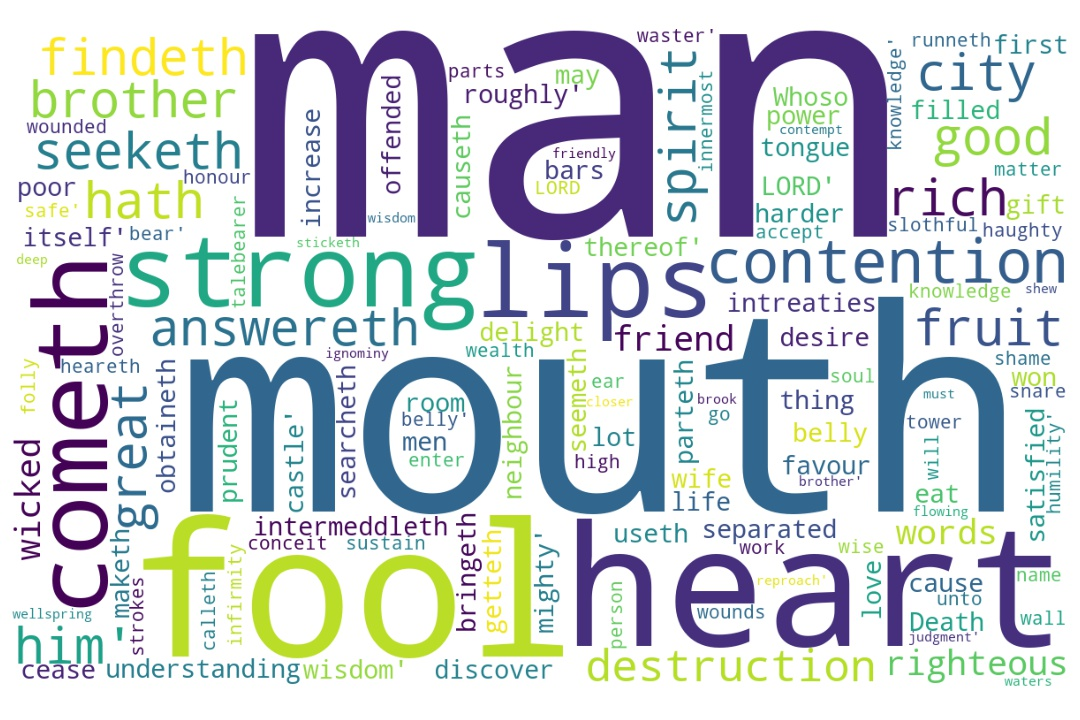
\includegraphics[width=\linewidth]{20OT-Proverbs/Proverb18-WordCloud.jpg}
  \caption{Proverb 18 Word Cloud}
  \label{fig:Proverb 18 word Cloud}
\end{figure}

\marginpar{\scriptsize \centering \fcolorbox{bone}{lime}{\textbf{A MAN FOCUSED ON GOD}}\\ (Proverbs 18:1-24) \begin{compactenum}[I.][8]
    \item Will be an \textbf{Inspired Man} - 
    \item Will be \textbf{Separate from the Ignorant Masses} - 
    \item For him most things in life will have  
    \textbf{Insignificant Meaning} - 
    \item Lives in an \textbf{Isolated Manner} 
    \item Lives by an \textbf{Individual Mandate} 
    \item Has an \textbf{intense and Insular Mentality}
\end{compactenum}}

\marginpar{\scriptsize \centering \fcolorbox{bone}{yellow}{\textbf{A FRIEND LIKE JESUS}}\\ (Proverb 18:24) \begin{compactenum}[I.][8]
    \item A \textbf{Close} Friend
    \item A \textbf{Constant} Friend
    \item A \textbf{Confiding} Friend
    \item A \textbf{Concerned} Friend
    \item A \textbf{Continuing} Friend
    \item A \textbf{Capable} Friend
    \item A \textbf{Caring} Friend
\end{compactenum}}

\marginpar{\scriptsize \centering \fcolorbox{bone}{black}{\textbf{\textcolor{white}{THE PURSUIT OF WISDOM}}}\\ (Proverb 18:24) \begin{compactenum}[I.][8]
    \item Then \textbf{Perverted} Motive -- to learn how manipulate events and circumstances. \index[scripture]{Proverbs!Pro 18:01}(Proverb 18:1)
    \item Then \textbf{Prideful} Motive -- To become exalted as wise. 
    \item Then \textbf{Public} Motive -- to be known and famous. 
    \item Then \textbf{Personal} Motive -- to achieve understanding. 
    \item Then \textbf{Practical} Motive -- to learn how live without mistakes or errors. 
    \item Then \textbf{Purposeful} Motive -- to learn navigate a specific problem. 
    \item Then \textbf{Perfect} Motive -- to learn how to live righteously before God. 
\end{compactenum}}

\marginpar{\scriptsize \centering \fcolorbox{bone}{blue}{\textbf{\textcolor{white}{WHAT YOUR SPEECH REVEALS}}}\\ (Proverb 18:4) \begin{compactenum}[I.][8]
    \item \textbf{Your Education} 
    \item \textbf{Your Excellence} 
    \item \textbf{Your Excitements} 
    \item \textbf{Your Enmity} 
    \item \textbf{Your Enemies} 
    \item \textbf{Your End} 
    \item \textbf{Your Emptiness}
    \item \textbf{Your Entanglements} 
\end{compactenum} }

\marginpar{\scriptsize \centering \fcolorbox{bone}{orange}{\textbf{THE WISE MAN}}\\ (Proverbs 18:1-24) \begin{compactenum}[I.][8]
    \item \textbf{Is Distinctive}
    \item \textbf{Is Disciplined}
    \item \textbf{Ignores Distractions}
    \item \textbf{Finds Delights in Wisdom}
    \item \textbf{Has Departed from the Common and Mundane}
    \item \textbf{Has a Distaste for Foolishness}
    \item \textbf{Is often regarded as Disturbed}
\end{compactenum} }




\footnote{\textcolor[cmyk]{0.99998,1,0,0}{\hyperlink{TOC}{Return to end of Table of Contents.}}}\footnote{\href{https://audiobible.com/bible/proverbs_18.html}{\textcolor[cmyk]{0.99998,1,0,0}{Proverbs Audio}}}\textcolor[cmyk]{0.99998,1,0,0}{Through desire a man, having separated himself, seeketh \emph{and} \fcolorbox{bone}{MYGOLD}{intermeddleth} with all wisdom.}
[2] \textcolor[cmyk]{0.99998,1,0,0}{A fool hath no delight in \fcolorbox{bone}{MYGOLD}{understanding}, but that \fcolorbox{bone}{bone}{his} heart may discover itself.}
[3] \textcolor[cmyk]{0.99998,1,0,0}{When the wicked cometh, \emph{then} cometh also contempt, and with ignominy reproach.}
[4] \textcolor[cmyk]{0.99998,1,0,0}{The words of a man's mouth \emph{are} \emph{as} deep waters, \emph{and} the wellspring of wisdom \emph{as} a flowing brook.}\footnote{\textbf{Proverb 16:22} - Understanding is a wellspring of life unto him that hath it: but the instruction of fools is folly.}
[5] \textcolor[cmyk]{0.99998,1,0,0}{\emph{It} \emph{is} not good to accept the person of the wicked, to overthrow the righteous in judgment.}
[6] \textcolor[cmyk]{0.99998,1,0,0}{A fool's lips enter into contention, and \fcolorbox{bone}{bone}{his} mouth calleth for strokes.}
[7] \textcolor[cmyk]{0.99998,1,0,0}{A fool's mouth \emph{is} \fcolorbox{bone}{bone}{his} destruction, and \fcolorbox{bone}{bone}{his} lips \emph{are} the snare of \fcolorbox{bone}{bone}{his} soul.}
[8] \textcolor[cmyk]{0.99998,1,0,0}{The words of a talebearer \emph{are} as wounds, and they go down into the innermost parts of the belly.}
[9] \textcolor[cmyk]{0.99998,1,0,0}{He also that is slothful in \fcolorbox{bone}{bone}{his} work is brother to him that is a great waster.}
[10] \textcolor[cmyk]{0.99998,1,0,0}{The name of the LORD \emph{is} a strong tower: the righteous runneth into it, and is safe.}
[11] \textcolor[cmyk]{0.99998,1,0,0}{The rich man's wealth \emph{is} \fcolorbox{bone}{bone}{his} strong city, and as an high wall in \fcolorbox{bone}{bone}{his} own conceit.}
[12] \textcolor[cmyk]{0.99998,1,0,0}{Before destruction the heart of man is haughty, and before honour \emph{is} humility.}
[13] \textcolor[cmyk]{0.99998,1,0,0}{He that answereth a matter before he heareth \emph{it}, it \emph{is} folly and shame unto him.}
[14] \textcolor[cmyk]{0.99998,1,0,0}{The spirit of a man will sustain \fcolorbox{bone}{bone}{his} infirmity; but a wounded spirit who can bear?}
[15] \textcolor[cmyk]{0.99998,1,0,0}{The heart of the prudent getteth knowledge; and the ear of the wise seeketh knowledge.}
[16] \textcolor[cmyk]{0.99998,1,0,0}{A man's gift maketh room for him, and bringeth him before great men.}
[17] \textcolor[cmyk]{0.99998,1,0,0}{\emph{He} \emph{that} \emph{is} first in \fcolorbox{bone}{bone}{his} own cause \emph{seemeth} just; but \fcolorbox{bone}{bone}{his} neighbour cometh and searcheth him.}
[18] \textcolor[cmyk]{0.99998,1,0,0}{The lot causeth contentions to cease, and parteth between the mighty.}
[19] \textcolor[cmyk]{0.99998,1,0,0}{A brother offended \emph{is} \emph{harder} \emph{to} \emph{be} \emph{won} than a strong city: and \emph{their} contentions \emph{are} like the bars of a castle.}
[20] \textcolor[cmyk]{0.99998,1,0,0}{A man's belly shall be satisfied with the fruit of \fcolorbox{bone}{bone}{his} mouth; \emph{and} with the increase of \fcolorbox{bone}{bone}{his} lips shall he be filled.}
[21] \textcolor[cmyk]{0.99998,1,0,0}{Death and life \emph{are} in the power of the tongue: and they that love it shall eat the fruit thereof.}
[22] \textcolor[cmyk]{0.99998,1,0,0}{\emph{Whoso} findeth a wife findeth a good \emph{thing}, and obtaineth favour of the LORD.}
[23] \textcolor[cmyk]{0.99998,1,0,0}{The poor useth intreaties; but the rich answereth roughly.}
[24] \textcolor[cmyk]{0.99998,1,0,0}{A man \emph{that} \emph{hath} friends must shew himself friendly: and there is a friend \emph{that} sticketh closer than a brother.}



\index[NWIV]{13!Proverbs!Pro 18:1}\index[AWIP]{Through!Proverbs!Pro 18:1}\index[AWIP]{desire!Proverbs!Pro 18:1}\index[AWIP]{a!Proverbs!Pro 18:1}\index[AWIP]{man!Proverbs!Pro 18:1}\index[AWIP]{having!Proverbs!Pro 18:1}\index[AWIP]{separated!Proverbs!Pro 18:1}\index[AWIP]{himself!Proverbs!Pro 18:1}\index[AWIP]{seeketh!Proverbs!Pro 18:1}\index[AWIP]{\emph{and}!Proverbs!Pro 18:1}\index[AWIP]{intermeddleth!Proverbs!Pro 18:1}\index[AWIP]{with!Proverbs!Pro 18:1}\index[AWIP]{all!Proverbs!Pro 18:1}\index[AWIP]{wisdom!Proverbs!Pro 18:1}\index[AWIP]{\emph{and}!Proverbs!Pro 18:1}

\index[NWIV]{14!Proverbs!Pro 18:2}\index[AWIP]{A!Proverbs!Pro 18:2}\index[AWIP]{fool!Proverbs!Pro 18:2}\index[AWIP]{hath!Proverbs!Pro 18:2}\index[AWIP]{no!Proverbs!Pro 18:2}\index[AWIP]{delight!Proverbs!Pro 18:2}\index[AWIP]{in!Proverbs!Pro 18:2}\index[AWIP]{understanding!Proverbs!Pro 18:2}\index[AWIP]{but!Proverbs!Pro 18:2}\index[AWIP]{that!Proverbs!Pro 18:2}\index[AWIP]{his!Proverbs!Pro 18:2}\index[AWIP]{heart!Proverbs!Pro 18:2}\index[AWIP]{may!Proverbs!Pro 18:2}\index[AWIP]{discover!Proverbs!Pro 18:2}\index[AWIP]{itself!Proverbs!Pro 18:2}

\index[NWIV]{12!Proverbs!Pro 18:3}\index[AWIP]{When!Proverbs!Pro 18:3}\index[AWIP]{the!Proverbs!Pro 18:3}\index[AWIP]{wicked!Proverbs!Pro 18:3}\index[AWIP]{cometh!Proverbs!Pro 18:3}\index[AWIP]{cometh!Proverbs!Pro 18:3 (2)}\index[AWIP]{\emph{then}!Proverbs!Pro 18:3}\index[AWIP]{also!Proverbs!Pro 18:3}\index[AWIP]{contempt!Proverbs!Pro 18:3}\index[AWIP]{and!Proverbs!Pro 18:3}\index[AWIP]{with!Proverbs!Pro 18:3}\index[AWIP]{ignominy!Proverbs!Pro 18:3}\index[AWIP]{reproach!Proverbs!Pro 18:3}\index[AWIP]{\emph{then}!Proverbs!Pro 18:3}

\index[NWIV]{19!Proverbs!Pro 18:4}\index[AWIP]{The!Proverbs!Pro 18:4}\index[AWIP]{words!Proverbs!Pro 18:4}\index[AWIP]{of!Proverbs!Pro 18:4}\index[AWIP]{of!Proverbs!Pro 18:4 (2)}\index[AWIP]{a!Proverbs!Pro 18:4}\index[AWIP]{a!Proverbs!Pro 18:4 (2)}\index[AWIP]{man's!Proverbs!Pro 18:4}\index[AWIP]{mouth!Proverbs!Pro 18:4}\index[AWIP]{\emph{are}!Proverbs!Pro 18:4}\index[AWIP]{\emph{as}!Proverbs!Pro 18:4}\index[AWIP]{\emph{as}!Proverbs!Pro 18:4 (2)}\index[AWIP]{deep!Proverbs!Pro 18:4}\index[AWIP]{waters!Proverbs!Pro 18:4}\index[AWIP]{\emph{and}!Proverbs!Pro 18:4}\index[AWIP]{the!Proverbs!Pro 18:4}\index[AWIP]{wellspring!Proverbs!Pro 18:4}\index[AWIP]{wisdom!Proverbs!Pro 18:4}\index[AWIP]{flowing!Proverbs!Pro 18:4}\index[AWIP]{brook!Proverbs!Pro 18:4}\index[AWIP]{\emph{are}!Proverbs!Pro 18:4}\index[AWIP]{\emph{as}!Proverbs!Pro 18:4}\index[AWIP]{\emph{as}!Proverbs!Pro 18:4 (2)}\index[AWIP]{\emph{and}!Proverbs!Pro 18:4}

\index[NWIV]{17!Proverbs!Pro 18:5}\index[AWIP]{\emph{It}!Proverbs!Pro 18:5}\index[AWIP]{\emph{is}!Proverbs!Pro 18:5}\index[AWIP]{not!Proverbs!Pro 18:5}\index[AWIP]{good!Proverbs!Pro 18:5}\index[AWIP]{to!Proverbs!Pro 18:5}\index[AWIP]{to!Proverbs!Pro 18:5 (2)}\index[AWIP]{accept!Proverbs!Pro 18:5}\index[AWIP]{the!Proverbs!Pro 18:5}\index[AWIP]{the!Proverbs!Pro 18:5 (2)}\index[AWIP]{the!Proverbs!Pro 18:5 (3)}\index[AWIP]{person!Proverbs!Pro 18:5}\index[AWIP]{of!Proverbs!Pro 18:5}\index[AWIP]{wicked!Proverbs!Pro 18:5}\index[AWIP]{overthrow!Proverbs!Pro 18:5}\index[AWIP]{righteous!Proverbs!Pro 18:5}\index[AWIP]{in!Proverbs!Pro 18:5}\index[AWIP]{judgment!Proverbs!Pro 18:5}\index[AWIP]{\emph{It}!Proverbs!Pro 18:5}\index[AWIP]{\emph{is}!Proverbs!Pro 18:5}

\index[NWIV]{12!Proverbs!Pro 18:6}\index[AWIP]{A!Proverbs!Pro 18:6}\index[AWIP]{fool's!Proverbs!Pro 18:6}\index[AWIP]{lips!Proverbs!Pro 18:6}\index[AWIP]{enter!Proverbs!Pro 18:6}\index[AWIP]{into!Proverbs!Pro 18:6}\index[AWIP]{contention!Proverbs!Pro 18:6}\index[AWIP]{and!Proverbs!Pro 18:6}\index[AWIP]{his!Proverbs!Pro 18:6}\index[AWIP]{mouth!Proverbs!Pro 18:6}\index[AWIP]{calleth!Proverbs!Pro 18:6}\index[AWIP]{for!Proverbs!Pro 18:6}\index[AWIP]{strokes!Proverbs!Pro 18:6}

\index[NWIV]{15!Proverbs!Pro 18:7}\index[AWIP]{A!Proverbs!Pro 18:7}\index[AWIP]{fool's!Proverbs!Pro 18:7}\index[AWIP]{mouth!Proverbs!Pro 18:7}\index[AWIP]{\emph{is}!Proverbs!Pro 18:7}\index[AWIP]{his!Proverbs!Pro 18:7}\index[AWIP]{his!Proverbs!Pro 18:7 (2)}\index[AWIP]{his!Proverbs!Pro 18:7 (3)}\index[AWIP]{destruction!Proverbs!Pro 18:7}\index[AWIP]{and!Proverbs!Pro 18:7}\index[AWIP]{lips!Proverbs!Pro 18:7}\index[AWIP]{\emph{are}!Proverbs!Pro 18:7}\index[AWIP]{the!Proverbs!Pro 18:7}\index[AWIP]{snare!Proverbs!Pro 18:7}\index[AWIP]{of!Proverbs!Pro 18:7}\index[AWIP]{soul!Proverbs!Pro 18:7}\index[AWIP]{\emph{is}!Proverbs!Pro 18:7}\index[AWIP]{\emph{are}!Proverbs!Pro 18:7}

\index[NWIV]{19!Proverbs!Pro 18:8}\index[AWIP]{The!Proverbs!Pro 18:8}\index[AWIP]{words!Proverbs!Pro 18:8}\index[AWIP]{of!Proverbs!Pro 18:8}\index[AWIP]{of!Proverbs!Pro 18:8 (2)}\index[AWIP]{a!Proverbs!Pro 18:8}\index[AWIP]{talebearer!Proverbs!Pro 18:8}\index[AWIP]{\emph{are}!Proverbs!Pro 18:8}\index[AWIP]{as!Proverbs!Pro 18:8}\index[AWIP]{wounds!Proverbs!Pro 18:8}\index[AWIP]{and!Proverbs!Pro 18:8}\index[AWIP]{they!Proverbs!Pro 18:8}\index[AWIP]{go!Proverbs!Pro 18:8}\index[AWIP]{down!Proverbs!Pro 18:8}\index[AWIP]{into!Proverbs!Pro 18:8}\index[AWIP]{the!Proverbs!Pro 18:8}\index[AWIP]{the!Proverbs!Pro 18:8 (2)}\index[AWIP]{innermost!Proverbs!Pro 18:8}\index[AWIP]{parts!Proverbs!Pro 18:8}\index[AWIP]{belly!Proverbs!Pro 18:8}\index[AWIP]{\emph{are}!Proverbs!Pro 18:8}

\index[NWIV]{17!Proverbs!Pro 18:9}\index[AWIP]{He!Proverbs!Pro 18:9}\index[AWIP]{also!Proverbs!Pro 18:9}\index[AWIP]{that!Proverbs!Pro 18:9}\index[AWIP]{that!Proverbs!Pro 18:9 (2)}\index[AWIP]{is!Proverbs!Pro 18:9}\index[AWIP]{is!Proverbs!Pro 18:9 (2)}\index[AWIP]{is!Proverbs!Pro 18:9 (3)}\index[AWIP]{slothful!Proverbs!Pro 18:9}\index[AWIP]{in!Proverbs!Pro 18:9}\index[AWIP]{his!Proverbs!Pro 18:9}\index[AWIP]{work!Proverbs!Pro 18:9}\index[AWIP]{brother!Proverbs!Pro 18:9}\index[AWIP]{to!Proverbs!Pro 18:9}\index[AWIP]{him!Proverbs!Pro 18:9}\index[AWIP]{a!Proverbs!Pro 18:9}\index[AWIP]{great!Proverbs!Pro 18:9}\index[AWIP]{waster!Proverbs!Pro 18:9}

\index[NWIV]{17!Proverbs!Pro 18:10}\index[AWIP]{The!Proverbs!Pro 18:10}\index[AWIP]{name!Proverbs!Pro 18:10}\index[AWIP]{of!Proverbs!Pro 18:10}\index[AWIP]{the!Proverbs!Pro 18:10}\index[AWIP]{the!Proverbs!Pro 18:10 (2)}\index[AWIP]{LORD!Proverbs!Pro 18:10}\index[AWIP]{\emph{is}!Proverbs!Pro 18:10}\index[AWIP]{a!Proverbs!Pro 18:10}\index[AWIP]{strong!Proverbs!Pro 18:10}\index[AWIP]{tower!Proverbs!Pro 18:10}\index[AWIP]{righteous!Proverbs!Pro 18:10}\index[AWIP]{runneth!Proverbs!Pro 18:10}\index[AWIP]{into!Proverbs!Pro 18:10}\index[AWIP]{it!Proverbs!Pro 18:10}\index[AWIP]{and!Proverbs!Pro 18:10}\index[AWIP]{is!Proverbs!Pro 18:10}\index[AWIP]{safe!Proverbs!Pro 18:10}\index[AWIP]{\emph{is}!Proverbs!Pro 18:10}

\index[NWIV]{17!Proverbs!Pro 18:11}\index[AWIP]{The!Proverbs!Pro 18:11}\index[AWIP]{rich!Proverbs!Pro 18:11}\index[AWIP]{man's!Proverbs!Pro 18:11}\index[AWIP]{wealth!Proverbs!Pro 18:11}\index[AWIP]{\emph{is}!Proverbs!Pro 18:11}\index[AWIP]{his!Proverbs!Pro 18:11}\index[AWIP]{his!Proverbs!Pro 18:11 (2)}\index[AWIP]{strong!Proverbs!Pro 18:11}\index[AWIP]{city!Proverbs!Pro 18:11}\index[AWIP]{and!Proverbs!Pro 18:11}\index[AWIP]{as!Proverbs!Pro 18:11}\index[AWIP]{an!Proverbs!Pro 18:11}\index[AWIP]{high!Proverbs!Pro 18:11}\index[AWIP]{wall!Proverbs!Pro 18:11}\index[AWIP]{in!Proverbs!Pro 18:11}\index[AWIP]{own!Proverbs!Pro 18:11}\index[AWIP]{conceit!Proverbs!Pro 18:11}\index[AWIP]{\emph{is}!Proverbs!Pro 18:11}

\index[NWIV]{13!Proverbs!Pro 18:12}\index[AWIP]{Before!Proverbs!Pro 18:12}\index[AWIP]{destruction!Proverbs!Pro 18:12}\index[AWIP]{the!Proverbs!Pro 18:12}\index[AWIP]{heart!Proverbs!Pro 18:12}\index[AWIP]{of!Proverbs!Pro 18:12}\index[AWIP]{man!Proverbs!Pro 18:12}\index[AWIP]{is!Proverbs!Pro 18:12}\index[AWIP]{haughty!Proverbs!Pro 18:12}\index[AWIP]{and!Proverbs!Pro 18:12}\index[AWIP]{before!Proverbs!Pro 18:12}\index[AWIP]{honour!Proverbs!Pro 18:12}\index[AWIP]{\emph{is}!Proverbs!Pro 18:12}\index[AWIP]{humility!Proverbs!Pro 18:12}\index[AWIP]{\emph{is}!Proverbs!Pro 18:12}

\index[NWIV]{16!Proverbs!Pro 18:13}\index[AWIP]{He!Proverbs!Pro 18:13}\index[AWIP]{that!Proverbs!Pro 18:13}\index[AWIP]{answereth!Proverbs!Pro 18:13}\index[AWIP]{a!Proverbs!Pro 18:13}\index[AWIP]{matter!Proverbs!Pro 18:13}\index[AWIP]{before!Proverbs!Pro 18:13}\index[AWIP]{he!Proverbs!Pro 18:13}\index[AWIP]{heareth!Proverbs!Pro 18:13}\index[AWIP]{\emph{it}!Proverbs!Pro 18:13}\index[AWIP]{it!Proverbs!Pro 18:13}\index[AWIP]{\emph{is}!Proverbs!Pro 18:13}\index[AWIP]{folly!Proverbs!Pro 18:13}\index[AWIP]{and!Proverbs!Pro 18:13}\index[AWIP]{shame!Proverbs!Pro 18:13}\index[AWIP]{unto!Proverbs!Pro 18:13}\index[AWIP]{him!Proverbs!Pro 18:13}\index[AWIP]{\emph{it}!Proverbs!Pro 18:13}\index[AWIP]{\emph{is}!Proverbs!Pro 18:13}

\index[NWIV]{16!Proverbs!Pro 18:14}\index[AWIP]{The!Proverbs!Pro 18:14}\index[AWIP]{spirit!Proverbs!Pro 18:14}\index[AWIP]{spirit!Proverbs!Pro 18:14 (2)}\index[AWIP]{of!Proverbs!Pro 18:14}\index[AWIP]{a!Proverbs!Pro 18:14}\index[AWIP]{a!Proverbs!Pro 18:14 (2)}\index[AWIP]{man!Proverbs!Pro 18:14}\index[AWIP]{will!Proverbs!Pro 18:14}\index[AWIP]{sustain!Proverbs!Pro 18:14}\index[AWIP]{his!Proverbs!Pro 18:14}\index[AWIP]{infirmity!Proverbs!Pro 18:14}\index[AWIP]{but!Proverbs!Pro 18:14}\index[AWIP]{wounded!Proverbs!Pro 18:14}\index[AWIP]{who!Proverbs!Pro 18:14}\index[AWIP]{can!Proverbs!Pro 18:14}\index[AWIP]{bear?!Proverbs!Pro 18:14}

\index[NWIV]{15!Proverbs!Pro 18:15}\index[AWIP]{The!Proverbs!Pro 18:15}\index[AWIP]{heart!Proverbs!Pro 18:15}\index[AWIP]{of!Proverbs!Pro 18:15}\index[AWIP]{of!Proverbs!Pro 18:15 (2)}\index[AWIP]{the!Proverbs!Pro 18:15}\index[AWIP]{the!Proverbs!Pro 18:15 (2)}\index[AWIP]{the!Proverbs!Pro 18:15 (3)}\index[AWIP]{prudent!Proverbs!Pro 18:15}\index[AWIP]{getteth!Proverbs!Pro 18:15}\index[AWIP]{knowledge!Proverbs!Pro 18:15}\index[AWIP]{knowledge!Proverbs!Pro 18:15 (2)}\index[AWIP]{and!Proverbs!Pro 18:15}\index[AWIP]{ear!Proverbs!Pro 18:15}\index[AWIP]{wise!Proverbs!Pro 18:15}\index[AWIP]{seeketh!Proverbs!Pro 18:15}

\index[NWIV]{13!Proverbs!Pro 18:16}\index[AWIP]{A!Proverbs!Pro 18:16}\index[AWIP]{man's!Proverbs!Pro 18:16}\index[AWIP]{gift!Proverbs!Pro 18:16}\index[AWIP]{maketh!Proverbs!Pro 18:16}\index[AWIP]{room!Proverbs!Pro 18:16}\index[AWIP]{for!Proverbs!Pro 18:16}\index[AWIP]{him!Proverbs!Pro 18:16}\index[AWIP]{him!Proverbs!Pro 18:16 (2)}\index[AWIP]{and!Proverbs!Pro 18:16}\index[AWIP]{bringeth!Proverbs!Pro 18:16}\index[AWIP]{before!Proverbs!Pro 18:16}\index[AWIP]{great!Proverbs!Pro 18:16}\index[AWIP]{men!Proverbs!Pro 18:16}

\index[NWIV]{17!Proverbs!Pro 18:17}\index[AWIP]{\emph{He}!Proverbs!Pro 18:17}\index[AWIP]{\emph{that}!Proverbs!Pro 18:17}\index[AWIP]{\emph{is}!Proverbs!Pro 18:17}\index[AWIP]{first!Proverbs!Pro 18:17}\index[AWIP]{in!Proverbs!Pro 18:17}\index[AWIP]{his!Proverbs!Pro 18:17}\index[AWIP]{his!Proverbs!Pro 18:17 (2)}\index[AWIP]{own!Proverbs!Pro 18:17}\index[AWIP]{cause!Proverbs!Pro 18:17}\index[AWIP]{\emph{seemeth}!Proverbs!Pro 18:17}\index[AWIP]{just!Proverbs!Pro 18:17}\index[AWIP]{but!Proverbs!Pro 18:17}\index[AWIP]{neighbour!Proverbs!Pro 18:17}\index[AWIP]{cometh!Proverbs!Pro 18:17}\index[AWIP]{and!Proverbs!Pro 18:17}\index[AWIP]{searcheth!Proverbs!Pro 18:17}\index[AWIP]{him!Proverbs!Pro 18:17}\index[AWIP]{\emph{He}!Proverbs!Pro 18:17}\index[AWIP]{\emph{that}!Proverbs!Pro 18:17}\index[AWIP]{\emph{is}!Proverbs!Pro 18:17}\index[AWIP]{\emph{seemeth}!Proverbs!Pro 18:17}

\index[NWIV]{11!Proverbs!Pro 18:18}\index[AWIP]{The!Proverbs!Pro 18:18}\index[AWIP]{lot!Proverbs!Pro 18:18}\index[AWIP]{causeth!Proverbs!Pro 18:18}\index[AWIP]{contentions!Proverbs!Pro 18:18}\index[AWIP]{to!Proverbs!Pro 18:18}\index[AWIP]{cease!Proverbs!Pro 18:18}\index[AWIP]{and!Proverbs!Pro 18:18}\index[AWIP]{parteth!Proverbs!Pro 18:18}\index[AWIP]{between!Proverbs!Pro 18:18}\index[AWIP]{the!Proverbs!Pro 18:18}\index[AWIP]{mighty!Proverbs!Pro 18:18}

\index[NWIV]{22!Proverbs!Pro 18:19}\index[AWIP]{A!Proverbs!Pro 18:19}\index[AWIP]{brother!Proverbs!Pro 18:19}\index[AWIP]{offended!Proverbs!Pro 18:19}\index[AWIP]{\emph{is}!Proverbs!Pro 18:19}\index[AWIP]{\emph{harder}!Proverbs!Pro 18:19}\index[AWIP]{\emph{to}!Proverbs!Pro 18:19}\index[AWIP]{\emph{be}!Proverbs!Pro 18:19}\index[AWIP]{\emph{won}!Proverbs!Pro 18:19}\index[AWIP]{than!Proverbs!Pro 18:19}\index[AWIP]{a!Proverbs!Pro 18:19}\index[AWIP]{a!Proverbs!Pro 18:19 (2)}\index[AWIP]{strong!Proverbs!Pro 18:19}\index[AWIP]{city!Proverbs!Pro 18:19}\index[AWIP]{and!Proverbs!Pro 18:19}\index[AWIP]{\emph{their}!Proverbs!Pro 18:19}\index[AWIP]{contentions!Proverbs!Pro 18:19}\index[AWIP]{\emph{are}!Proverbs!Pro 18:19}\index[AWIP]{like!Proverbs!Pro 18:19}\index[AWIP]{the!Proverbs!Pro 18:19}\index[AWIP]{bars!Proverbs!Pro 18:19}\index[AWIP]{of!Proverbs!Pro 18:19}\index[AWIP]{castle!Proverbs!Pro 18:19}\index[AWIP]{\emph{is}!Proverbs!Pro 18:19}\index[AWIP]{\emph{harder}!Proverbs!Pro 18:19}\index[AWIP]{\emph{to}!Proverbs!Pro 18:19}\index[AWIP]{\emph{be}!Proverbs!Pro 18:19}\index[AWIP]{\emph{won}!Proverbs!Pro 18:19}\index[AWIP]{\emph{their}!Proverbs!Pro 18:19}\index[AWIP]{\emph{are}!Proverbs!Pro 18:19}

\index[NWIV]{23!Proverbs!Pro 18:20}\index[AWIP]{A!Proverbs!Pro 18:20}\index[AWIP]{man's!Proverbs!Pro 18:20}\index[AWIP]{belly!Proverbs!Pro 18:20}\index[AWIP]{shall!Proverbs!Pro 18:20}\index[AWIP]{shall!Proverbs!Pro 18:20 (2)}\index[AWIP]{be!Proverbs!Pro 18:20}\index[AWIP]{be!Proverbs!Pro 18:20 (2)}\index[AWIP]{satisfied!Proverbs!Pro 18:20}\index[AWIP]{with!Proverbs!Pro 18:20}\index[AWIP]{with!Proverbs!Pro 18:20 (2)}\index[AWIP]{the!Proverbs!Pro 18:20}\index[AWIP]{the!Proverbs!Pro 18:20 (2)}\index[AWIP]{fruit!Proverbs!Pro 18:20}\index[AWIP]{of!Proverbs!Pro 18:20}\index[AWIP]{of!Proverbs!Pro 18:20 (2)}\index[AWIP]{his!Proverbs!Pro 18:20}\index[AWIP]{his!Proverbs!Pro 18:20 (2)}\index[AWIP]{mouth!Proverbs!Pro 18:20}\index[AWIP]{\emph{and}!Proverbs!Pro 18:20}\index[AWIP]{increase!Proverbs!Pro 18:20}\index[AWIP]{lips!Proverbs!Pro 18:20}\index[AWIP]{he!Proverbs!Pro 18:20}\index[AWIP]{filled!Proverbs!Pro 18:20}\index[AWIP]{\emph{and}!Proverbs!Pro 18:20}

\index[NWIV]{20!Proverbs!Pro 18:21}\index[AWIP]{Death!Proverbs!Pro 18:21}\index[AWIP]{and!Proverbs!Pro 18:21}\index[AWIP]{and!Proverbs!Pro 18:21 (2)}\index[AWIP]{life!Proverbs!Pro 18:21}\index[AWIP]{\emph{are}!Proverbs!Pro 18:21}\index[AWIP]{in!Proverbs!Pro 18:21}\index[AWIP]{the!Proverbs!Pro 18:21}\index[AWIP]{the!Proverbs!Pro 18:21 (2)}\index[AWIP]{the!Proverbs!Pro 18:21 (3)}\index[AWIP]{power!Proverbs!Pro 18:21}\index[AWIP]{of!Proverbs!Pro 18:21}\index[AWIP]{tongue!Proverbs!Pro 18:21}\index[AWIP]{they!Proverbs!Pro 18:21}\index[AWIP]{that!Proverbs!Pro 18:21}\index[AWIP]{love!Proverbs!Pro 18:21}\index[AWIP]{it!Proverbs!Pro 18:21}\index[AWIP]{shall!Proverbs!Pro 18:21}\index[AWIP]{eat!Proverbs!Pro 18:21}\index[AWIP]{fruit!Proverbs!Pro 18:21}\index[AWIP]{thereof!Proverbs!Pro 18:21}\index[AWIP]{\emph{are}!Proverbs!Pro 18:21}

\index[NWIV]{14!Proverbs!Pro 18:22}\index[AWIP]{\emph{Whoso}!Proverbs!Pro 18:22}\index[AWIP]{findeth!Proverbs!Pro 18:22}\index[AWIP]{findeth!Proverbs!Pro 18:22 (2)}\index[AWIP]{a!Proverbs!Pro 18:22}\index[AWIP]{a!Proverbs!Pro 18:22 (2)}\index[AWIP]{wife!Proverbs!Pro 18:22}\index[AWIP]{good!Proverbs!Pro 18:22}\index[AWIP]{\emph{thing}!Proverbs!Pro 18:22}\index[AWIP]{and!Proverbs!Pro 18:22}\index[AWIP]{obtaineth!Proverbs!Pro 18:22}\index[AWIP]{favour!Proverbs!Pro 18:22}\index[AWIP]{of!Proverbs!Pro 18:22}\index[AWIP]{the!Proverbs!Pro 18:22}\index[AWIP]{LORD!Proverbs!Pro 18:22}\index[AWIP]{\emph{Whoso}!Proverbs!Pro 18:22}\index[AWIP]{\emph{thing}!Proverbs!Pro 18:22}

\index[NWIV]{9!Proverbs!Pro 18:23}\index[AWIP]{The!Proverbs!Pro 18:23}\index[AWIP]{poor!Proverbs!Pro 18:23}\index[AWIP]{useth!Proverbs!Pro 18:23}\index[AWIP]{intreaties!Proverbs!Pro 18:23}\index[AWIP]{but!Proverbs!Pro 18:23}\index[AWIP]{the!Proverbs!Pro 18:23}\index[AWIP]{rich!Proverbs!Pro 18:23}\index[AWIP]{answereth!Proverbs!Pro 18:23}\index[AWIP]{roughly!Proverbs!Pro 18:23}

\index[NWIV]{20!Proverbs!Pro 18:24}\index[AWIP]{A!Proverbs!Pro 18:24}\index[AWIP]{man!Proverbs!Pro 18:24}\index[AWIP]{\emph{that}!Proverbs!Pro 18:24}\index[AWIP]{\emph{that}!Proverbs!Pro 18:24 (2)}\index[AWIP]{\emph{hath}!Proverbs!Pro 18:24}\index[AWIP]{friends!Proverbs!Pro 18:24}\index[AWIP]{must!Proverbs!Pro 18:24}\index[AWIP]{shew!Proverbs!Pro 18:24}\index[AWIP]{himself!Proverbs!Pro 18:24}\index[AWIP]{friendly!Proverbs!Pro 18:24}\index[AWIP]{and!Proverbs!Pro 18:24}\index[AWIP]{there!Proverbs!Pro 18:24}\index[AWIP]{is!Proverbs!Pro 18:24}\index[AWIP]{a!Proverbs!Pro 18:24}\index[AWIP]{a!Proverbs!Pro 18:24 (2)}\index[AWIP]{friend!Proverbs!Pro 18:24}\index[AWIP]{sticketh!Proverbs!Pro 18:24}\index[AWIP]{closer!Proverbs!Pro 18:24}\index[AWIP]{than!Proverbs!Pro 18:24}\index[AWIP]{brother!Proverbs!Pro 18:24}\index[AWIP]{\emph{that}!Proverbs!Pro 18:24}\index[AWIP]{\emph{that}!Proverbs!Pro 18:24 (2)}\index[AWIP]{\emph{hath}!Proverbs!Pro 18:24}


\section{Proverb 18 Outlines}

\subsection{My Outlines}

\subsubsection{A Man Focused on God's Wisdom}
\index[speaker]{Keith Anthony!Proverb 18 (A Man Focused on God's Wisdom)}
\index[series]{Proverbs (Keith Anthony)!Pro 18 (A Man Focused on God's Wisdom)}
\index[date]{2014/11/18!Proverb 18 (A Man Focused on God's Wisdom) (Keith Anthony)}
Proverbs 18:1 gives some hints about a man who is ostensibly focused on getting God's wisdom. Can we relate to this kind of person? Do we have any biblical examples? Could it be Elijah, or John the Baptist?
\begin{compactenum}[I.]
    \item Will be an \textbf{Inspired Man} - 
    \item Will be \textbf{Separate from the Ignorant Masses} - 
    \item For him most things in life will have  \textbf{Insignificant Meaning} - 
    \item Lives in an \textbf{Isolated Manner} 
    \item Lives by an \textbf{Individual Mandate} -  seldom supported by friends, and 
    \item Has an \textbf{intense and Insular Mentality} - 
\end{compactenum}
So, this is a guy who is mostly unwanted and unwelcome. Vast majority cannot related to him. How much are you like this man? How much do you want to be? How much do you think you should be?

\subsubsection{A Friend Like Jesus}
\index[speaker]{Keith Anthony!Proverb 18 (A Friend Like Jesus)}
\index[series]{Proverbs (Keith Anthony)!Pro 18 (A Friend Like Jesus)}
\index[date]{2014/11/18!Proverb 18 (A Friend Like Jesus (Keith Anthony)}
\begin{compactenum}[I.][8]
    \item A \textbf{Close} Friend
    \item A \textbf{Constant} Friend
    \item A \textbf{Confiding} Friend
    \item A \textbf{Concerned} Friend
    \item A \textbf{Continuing} Friend
    \item A \textbf{Capable} Friend
    \item A \textbf{Caring} Friend
\end{compactenum}


\subsubsection{The Pursuit of Wisdom}
\index[speaker]{Keith Anthony!Proverb 18 (The Pursuit of Wisdom)}
\index[series]{Proverbs (Keith Anthony)!Pro 18 (The Pursuit of Wisdom)}
\index[date]{2017/03/18!Proverb 18:01 (The Pursuit of Wisdom) (Keith Anthony)}
At issue in the pursuit of wisdom, is the underlying heart motive. I contest that ``Wisdom'' is not a thing, but a person, an individual, who is reading our motives as we go. I also contest that going to wisdom with the wrong motive could lead to disastrous results. Motives range from 100 per cent evil, to (seldom if ever) 100 per cent right. Some of these motives:
\begin{compactenum}[I.]
    \item Then \textbf{Perverted} Motive -- to learn how manipulate events and circumstances. \index[scripture]{Proverbs!Pro 18:01}(Proverb 18:1)
    \item Then \textbf{Prideful} Motive -- To become exalted as wise. 
    \item Then \textbf{Public} Motive -- to be known and famous. 
    \item Then \textbf{Personal} Motive -- to achieve understanding. 
    \item Then \textbf{Practical} Motive -- to learn how live without mistakes or errors. 
    \item Then \textbf{Purposeful} Motive -- to learn navigate a specific problem. 
    \item Then \textbf{Perfect} Motive -- to learn how to live righteously before God. 
\end{compactenum}

\subsubsection{What Your Speech Reveals}
My other main text will be James 3:3-10. which I will quote:  Behold, we put bits in the horses’ mouths, that they may obey us; and we turn about their whole body. [4] Behold also the ships, which though they be so great, and are driven of fierce winds, yet are they turned about with a very small helm, whithersoever the governor listeth. [5] Even so the tongue is a little member, and boasteth great things. Behold, how great a matter a little fire kindleth! [6] And the tongue is a fire, a world of iniquity: so is the tongue among our members, that it defileth the whole body, and setteth on fire the course of nature; and it is set on fire of hell. [7] For every kind of beasts, and of birds, and of serpents, and of things in the sea, is tamed, and hath been tamed of mankind: [8] But the tongue can no man tame; it is an unruly evil, full of deadly poison. [9] Therewith bless we God, even the Father; and therewith curse we men, which are made after the similitude of God. [10] Out of the same mouth proceedeth blessing and cursing. My brethren, these things ought not so to be. [11] Doth a fountain send forth at the same place sweet water and bitter? 12 Can the fig tree, my brethren, bear olive berries? either a vine, figs? so can no fountain both yield salt water and fresh.\\
\\
Consider the verses Proverbs 18:4, Proverbs 18:6, Proverbs 18:7, Proverbs 18:8, and Proverbs 18:13.  These verses say a lot about what people say. What does your speech reveal? Listen to someone long enough and their tongue will betray their innermost secrets ... The things that they love... The things that they focus on... It will reveal if they swim with the deep thinkers or wade in the shallow end of the pool with the other immature and self-focused babies ... Your concept of God, Christianity, and spiritual truth will eventually be reflected in your speech, in casual conversation ... Matthew 26:73, speaking of Peter's denial of Christ, says: And after a while came unto him they that stood by, and said to Peter, Surely thou also art one of them; for thy speech bewrayeth thee.\\
\\
Some things your tongue will tell about you:
\index[speaker]{Keith Anthony!Proverb 18:04 (What Your Speech Reveals)}\\
\index[series]{Proverbs (Keith Anthony)!Pro 18 (What Your Speech Reveals)}
\index[date]{2014/10/18!Proverb 18 (What Your Speech Reveals) (Keith Anthony)}

\index[LOCATION]{Greene County Adult Detention Center!2022/01/18!Tuesday Night}

\begin{compactenum}[I.][10]
    \item \textbf{Your Education} Do you use bad grammar? Intentionally?  Do you use Ebonics?  Is every word, or every other word, out of your mouth a cuss word?  When I say, though, what I really mean is wisdom. 
    \item \textbf{Your Excellence} Or lack of excellence ... If you are a child of God, you are a child of THE King and should talk like it. Back it Daniel 6:3 scripture says, ``Then this Daniel was preferred above the presidents and princes, because an excellent spirit was in him; and the king thought to set him over the whole realm.'' Proverbs 8:6 says: ``Hear; for I will speak of excellent things; and the opening of my lips shall be right things.''
    \item \textbf{Your Excitements} -- what gets you going
    \item \textbf{Your Enmity} -- So, you just can't help with this one ... At some point you're going to speak up on the things that irritate you 
    \item \textbf{Your Enemies} -- who you just might hurt if you had the chance.. But scripture says to let the Lord have vengeance. Nahum 1:2 says: God is jealous, and the LORD revengeth; the LORD revengeth, and is furious; the LORD will take vengeance on his adversaries, and he reserveth wrath for his enemies.
    \item \textbf{Your Enticements} What about that new Corvette?  How about that new Tesla.  I'd sure have fun shooting an AR-15 ... Whata about that new Movie ... and the lead actress?
    \item \textbf{Your Entanglements} -- what preoccupies you is what has you in chains
    \item \textbf{Your Emptiness} A while ago I saw an old friend, who attends a church I used to go to, and who I had not seen in about 5 years. I was expecting a warm ``glad to see you'', but instead got some comment about still being overweight. I guess that gives a measure of that friendship.  Getting more personal, ow many times have we asked ``how are you?'' when we really were not interested in the answer? We spend a great ... Do you or I speak of things that have substance? The problem is that the unsaved really have nothing of substance.
   \item \textbf{Your End} considering the rest of Proverbs, it if usually clear where your road is headed ... Christians often, sometimes usually, talk about heaven.  The lost talk about everything except heaven.  
\end{compactenum}
Matthew 12:36-37 tells us: ``But I say unto you, That every idle word that men shall speak, they shall give account thereof in the day of judgment. [37] For by thy words thou shalt be justified, and by thy words thou shalt be condemned.''\\
\\
So, (1) Consider, (2) Correct, (3) Covert, (4) Control, (5)

\subsubsection{The Wise Man}
\index[speaker]{Keith Anthony!Proverb 18 (The Wise Man)}
\index[series]{Proverbs (Keith Anthony)!Pro 18 (The Wise Man)}
\index[date]{2014/11/18!Proverb 18 (The Wise Man) (Keith Anthony)}
Proverbs 18:1 gives some hints about a wise man:
\begin{compactenum}[I.]
    \item \textbf{Is Distinctive}
    \item \textbf{Is Disciplined}
    \item \textbf{Ignores Distractions}
    \item \textbf{Finds Delights in Wisdom}
    \item \textbf{Has Departed from the Common and Mundane}
    \item \textbf{Has a Distaste for Foolishness}
    \item \textbf{Is often regarded as Disturbed}
\end{compactenum}


\subsection{Outlines from Billheimer}

\subsubsection{What a Friend}
\index[speaker]{Clarence Billheimer!Proverbs 18:24 (What a Friend)}
\index[series]{Proverbs (Clarence Billheimer)!Proverbs 18:24 (What a Friend)}
\index[date]{2015/04/12!Pro 18:24 (What a Friend) (Clarence Billheimer)}

\noindent  \textbf{Introduction: } How many of you have friends? How about close friends? How many of you ever lost a friend (other than by death)? How about a close friend? Someone said we can count our true friends on one hand. Having a true friend is really more rare than we think. But the Bible tells us about the Lord Jesus Christ, a true friend, one, who as this passage says, ``sticks closer than a brother.'' Let us look at six things about this true friend, using the letters of the word friend.
\begin{compactenum}[I.]
    \item \textbf{He is faithful} \index[scripture]{1 John!1 John 1:09}(1 John 1:9)
    \item \textbf{He is our redeemer} \index[scripture]{Job!Job 19:25}(Job 19:25)
    \item \textbf{He is interested} \index[scripture]{Philippians!Phil 4:06}(Phil 4:6)
    \item \textbf{He is empathetic} \index[scripture]{Hebrews!Heb 04:15}(Heb 4:15)
    \item \textbf{He is near} \index[scripture]{Hebrews!Heb 13:05}(Heb 13:5)
    \item \textbf{He is our deliverer} (\index[scripture]{2 Samuel!2 Sam 22:02}2 Samuel 22:2, \index[scripture]{Psalm!Psa 18:02}Psalm 18:2)
\end{compactenum}
\textbf{Conclusion: } There are many other things about Jesus Christ that make Him a very special friend. Do you know Him as not only a friend, but as your Savior?



\index[FACEBOOK]{FUNDAMENTAL BAPTIST SERMON OUTLINES!Clarence Billheimer (What a Friend) - Proverbs 18:24!2015/04/12}
\subsection{Outlines from Jimmy Chapman}

\subsubsection{Friendship}

\index[speaker]{Jimmy Chapman!Proverb 18:24 (Friendship)}
\index[series]{Proverbs (Jimmy Chapman)!Pro 18:24 (Friendship)}
\index[date]{2019/08/21!Pro 18:24 (Friendship) (Jimmy Chapman)}

%\noindent  \textbf{Introduction: } 

\begin{compactenum}[I.]
    \item how to develop  - Proverbs 18:24
    \item how to determine - Proverbs 17:17
    \item how to destroy - Proverbs 17:18
\end{compactenum}
%\textbf{Conclusion: } 



\index[FACEBOOK]{FUNDAMENTAL BAPTIST SERMON OUTLINES!Jimmy Chapman - Proverb 18:24!2019/08/21}
\subsection{Outlines from Doug McDaris}

\subsubsection{Five Different Types Of Friendships In The Book Of Proverbs}

\index[speaker]{Doug McDaris!Proverb 18:24 (Five Different Types Of Friendships In The Book Of Proverbs)}
\index[series]{Proverbs (Doug McDaris)!Pro 18:24 (Five Different Types Of Friendships In The Book Of Proverbs)}
\index[date]{2014/01/05!Pro 18:24 (Five Different Types Of Friendships In The Book Of Proverbs) (Doug McDaris)}

\noindent  \textbf{Introduction: } 
\begin{compactenum}[A.]
    \item There Is False Friendships (Proverb 14:20, Proverb 19:4, Proverb 19:6)
    \item There Is Fractured  Friendships (Proverb 16:28, Proverb 17:9)
    \item There Is Faithful  Friendships (Proverb 17:17, Proverb 27:10)
    \item There Is Forbidden  Friendships (Proverb 22:24-25)
    \item There Is Fearful Friendships (Proverb 27:17)\\
\end{compactenum}
The Friendship Of Jesus Christ\\
\\
\begin{compactenum}[I.]
    \item The Friendship Of Jesus Christ Is A Loving Friendship
    \begin{compactenum}[A.]
        \item This Friendship Is Based Upon An Unconditional Love.
        \item This Friendship Is Based Upon An Uncommon Loyalty.
    \end{compactenum}
    \item The Friendship Of Jesus Christ Is A Lasting Friendship.
    \begin{compactenum}[A.]
        \item This Friendship Is Based Upon His Readiness To Forgive.
        \item This Friendship Is Based Upon His Reluctance To Fault-Finding.
    \end{compactenum}
    \item The Friendship Of Jesus Christ Is A Legitimate Friendship
    \begin{compactenum}[A.]
        \item This Friendship Is Based Upon The Integrity Of His Character.
        \item This Friendship Is Based Upon The Impeccability Of His Character.
    \end{compactenum}
\end{compactenum}
%\textbf{Conclusion: } 



\index[FACEBOOK]{ALLITERATED SERMON OUTLINES!Doug McDaris - Proverb 18:24!2014/01/05}
\subsection{Outlines from Richard Drummond}

\subsubsection{What a Friend}

\index[speaker]{Richard Drummond!Proverbs 18:24 (What a Friend)}
\index[series]{Proverbs (Richard Drummond)!Pro 18:24 What a Friend)}

\index[date]{2017/17/13!Proverbs 18:24 (What a Friend) (Richard Drummond)}
\noindent \textbf{Introduction: } Friends make this life much more enjoyable. There is nothing like serving the Lord with brothers and sisters in Christ. Maybe you fish, hunt, or enjoy other types of activities with those you cherish in this life. We all have special people in our lives that we love to spend time with; however, our best friend should always be the Lord Jesus Christ. In times of trouble, grief, sorrow, and despair, Jesus has been there for you and I. In times of joy, happiness, excitement, and gain, Jesus has been there for you and I!
Notice several things with me about this friendship you and I ought to cherish:
%
\begin{compactenum}[I.]
    \item The \textbf{Availability} of a Friend\index[scripture]{Proverbs!Pro 18:24} (Proverb 18:24)
    \begin{compactenum}[A.]
    	\item Nature desires friends
    	\item Need demands friends
    \end{compactenum}
    \item The \textbf{Attributes} of a Friend\index[scripture]{Proverbs!Pro 18:24} (Proverb 18:24)
    \begin{compactenum}[A.]
    	\item Sympathetic touched when mistreated, sorrow, loss, cries, misunderstood
    	\item Steadfast - there all the time \index[scripture]{Proverbs!Pro 17:17} (Proverbs 17:17)
    	\item Strong
    \end{compactenum}
    \item The \textbf{Accessibility} of a Friend\index[scripture]{Proverbs!Pro 18:24} (Proverb 18:24)    \begin{compactenum}[A.]
    	\item He accepts us \index[scripture]{John!Jhn 6:37} (John. 6:37)
    	\item He affirms us \index[scripture]{1 John!1Jn 3:1} (1 John 3:1)
    	\item He assists \index[scripture]{Philippians!Phil 4:13} (Phil 4:13)
    \end{compactenum}
\end{compactenum}



\index[LOCATION]{Lebanon Baptist Temple (Drummond - What a Friend)!2017/7/13!Sunday Night}



\subsection{Outlines from Brian Eades}

\subsubsection{Finding A Wife Finding a Good Thing}

\index[speaker]{Brian Eades!Proverb 18:22 (Finding A Wife Finding a Good Thing)}
\index[series]{Proverbs (Brian Eades)!Pro 18:22 (Finding A Wife Finding a Good Thing)}
\index[date]{2018/10/22!Pro 18:22 (Finding A Wife Finding a Good Thing) (Brian Eades)}

\index[FACEBOOK]{SERMON HINTS!Brian Eades (Finding A Wife Finding a Good Thing) - Proverb 18:22!2018/10/22}

\noindent  \textbf{Introduction: } When God created everything, he said that it all was "very good" with the exception of one thing, and that was the loneliness of man. That was the only thing that God said was "not good". Shall we say that God makes things that aren't good so that good can come from it? 
That only seems to be the picture in the story of creation. I think the statement that man being alone was "not good" was God's way of saying that he was not finished with the full  (or complete) creation of Humanity as he intended it.
Here in the Book of Proverbs we have the statement that when man finds a wife he finds a good thing. I can tell of many instances where when a man found a wife it was the worst thing, but the overall picture here is that a man finds someone who honors God with their life and supports him, and helps complete him in life. God intended the woman to be a help that was meet for him, or right for him. There are many women that are NOT right for any man!\\
\\
*Finding a wife should be a: \\
\begin{compactenum}[I.]
    \item A \textbf{PRAYERFUL SEARCH}
    \item A \textbf{POSITIVE SEARCH}
    \item A \textbf{PATTERNED SEARCH}
    \item A \textbf{PROFITABLE SEARCH}
    \item A \textbf{PLEASING SEARCH}
\end{compactenum}

\subsection{Outlines from Hines}

\subsubsection{Jesus, My Best Friend}

\index[speaker]{Matthew Hines!Proverb 18:24 (Jesus, My Best Friend)}
\index[series]{Proverbs (Matthew Hines)!Pro 18:24 (Jesus, My Best Friend)}
\index[date]{2017/17/13!Proverb 18:24 (Jesus, My Best Friend) (Matthew Hines)}

\noindent  \textbf{Introduction: } Friends make this life much more enjoyable. There is nothing like serving the Lord with brothers and sisters in Christ. Maybe you fish, hunt, or enjoy other types of activities with those you cherish in this life. We all have special people in our lives that we love to spend time with; however, our best friend should always be the Lord Jesus Christ. In times of trouble, grief, sorrow, and despair, Jesus has been there for you and I. In times of joy, happiness, excitement, and gain, Jesus has been there for you and I!
Notice several things with me about this friendship you and I ought to cherish:
\begin{compactenum}[I.]
    \item The \textbf{PERSON of This Friendship: Gods SON} \index[scripture]{Proverbs!Pro 18:24} (Pro 18:24)
    \item The \textbf{PRICE of This Friendship: SACRIFICE} \index[scripture]{John!John 15:13} (John 15:13)
    \item The \textbf{POWER of This Friendship: Gives me STRENGTH} \index[scripture]{Philippians!Phil 04:13} (Phil 4:13)
    \item The \textbf{PERPETUITY of This Friendship: He is STEDFAST} \index[scripture]{Proverbs!Pro 17:17} (Pro 17:17)
    \item  \textbf{PROOF of This Friendship: SERVICE in His name} \index[scripture]{John!John 14:15} (John 14:15)
    \end{compactenum}
\textbf{Conclusion: } consider these thoughts from the scripture as you go throughout your day. Jesus is the greatest friend you have. He desires that you would know Him on a real and personal level. Do you know him today? If not make a new friend, the best friend you'll ever have!


\index[FACEBOOK]{FUNDAMENTAL BAPTIST SERMON OUTLINES!Matthew Hines - Proverb 18:24!2017/17/13}
\subsection{Outlines from J D Tyson}

\subsubsection{Jesus, what a friend is He}
\index[speaker]{J D Tyson!Proverb 18:24 (Jesus, what a friend is He)}
\index[series]{Proverbs (J D Tyson)!Pro 18:24 (Jesus, what a friend is He)}
\index[date]{2019/10/1!Pro 18:24 (Jesus, what a friend is He) (J D Tyson)}

\noindent  \textbf{Introduction: } How many of you have friends? How about close friends? How many of you ever lost a friend (other than by death)? How about a close friend? Someone said we can count our true friends on one hand. Having a true friend is really more rare than we think. But the Bible tells us about the Lord Jesus Christ, a true friend, one, who as this passage says, ``sticks closer than a brother.'' Let us look at six things about this true friend, using the letters of the word friend.
\begin{compactenum}[I.]
    \item A Limitless Friend – Matt 9:9-12
    \item A Loving Friend – John 11:1-11; 33-36
    \item A Loyal Friend – Matt 26:47-50
    \item A Lenient Friend – John 21:15-19
    \item A Life-giving Friend – John15:13
\end{compactenum}
%\textbf{Conclusion: } 



\index[FACEBOOK]{FUNDAMENTAL BAPTIST SERMON OUTLINES!J D Tyson - Proverb 18:24!2019/10/1}
\section{Proverb 18 Comments}

\subsection{Numerical Nuggets}
\textbf{13:} The word ``wellspring'' found only twice in scripture is the 13$^{th}$ word in verse 4. Two thirteen-letter words are in the chapter: ``intermeddleth'' and ``understanding.'' Verse 12, speaking of haughtiness, has 13 words. Verses 1, 12, and 16 have 13 words. Verses 7 and 12 have 13 unique words. The word ``his'' is used 13 times in the chapter. The 13-letter words ``intermeddleth'' and ``understanding'' are used in the chapter.

\subsection{Proverb 18:1-2}
The issue addressed in verses 1 and 2 is the human heart, and as such it should be expected that man will confront and change it, as shown in Table~\ref{table:CorruptionProv18:1}. The verse goes to motive. This is why most (or maybe all) research, ostensibly done for the betterment of mankind, eventually is used to oppress mankind. It comes down to power, position, prestige, prominence, and power. It comes down to why one seeks those things. Verse 2 puts the thought in context: it is the fool who trusts his heart and seeks the heart's desire. Why is this man a fool? It is because a sincere, God-seeking man will quickly elan from scripture the sordid details and depravity of the human heart.\footnote{\textbf{Isaiah 5:21} - Woe unto them that are wise in their own eyes, and prudent in their own sight!}\footnote{\textbf{Luke 10:21} - In that hour Jesus rejoiced in spirit, and said, I thank thee, O Father, Lord of heaven and earth, that thou hast hid these things from the wise and prudent, and hast revealed them unto babes: even so, Father; for so it seemed good in thy sight.}\\
\\
\noindent One commentator explains the process \cite{ruckman1972proverbs}:
\begin{compactenum}[1.]
    \item DESIRE is at the root of all scientific research and investigation (verse 1),
    \item This desire comes form the human HEART and not the human MIND (verse 2),
    \item This desire is essentially subjective, egotistical, and self-seeking (verse 2),
    \item This desire leads a man to pursue the life of isolated superiority, perhaps even the ivory towers of academic, or the esteemed halls of theological institutions, where he deep-down considers himself to be above the masses, or above the common folk. This may even start out as, or continue to masquerade as, a noble cause.
    \item The man does not seek wisdom. He ``seeketh and intermeddleth with all wisdom.'' 
    \item The man's ``love of wisdom'' is neither pure, not objective, not philanthropic.
    \item The wisdom ``sought'' is complete and is a mean's to an end.
\end{compactenum}

\newpage
\begin{center}

\begin{table}[ht]
\centering
\begin{tabular}{|p{.5in}|p{3.5in}|}
    \hline
    \textcolor{blue}{AV} & \textcolor{blue}{Through desire a man, having separated himself, seeketh \emph{and} intermeddleth with all wisdom.}\\ \hline
    \hline
    CEB &  Unfriendly people look out for themselves; they bicker with sensible people.\\ \hline
%
ESV & Whoever isolates himself seeks his own desire;  he breaks out against all sound judgment. \\ \hline
%
NASV &  He who separates himself seeks his own desire, He quarrels against all sound wisdom.\\ \hline
%
MEV & He who separates himself seeks his own desire; he seeks and quarrels against all wisdom.\\ \hline
%
NIV &  An unfriendly person pursues selfish ends and against all sound judgment starts quarrels. \\ \hline
%
NKJV &  A man who isolates himself seeks his own desire; He rages against all wise judgment.\\ \hline
%
RSV &  He who is estranged seeks pretexts  to break out against all sound judgment.\\ \hline \hline

\multicolumn{2}{|p{4.2in}|}{{\textcolor{jungle}{Modern translations, such as the ASV and others, strike out the first part of the verse, concealing the intent of mankind in general.  It goes to the heart's intent in seeking wisdom. How wonderful is the obfuscated RSV text: ``He who is estranged seeks pretexts.'' What does THAT mean?}}} \\ \hline

\end{tabular}
\caption[Corruption Alert: Proverb 18:1]{Corruption Alert: Proverb 18:1} \label{table:Corruption Proverb 18:1}
\end{table}

\end{center}


\newpage


\subsection{Proverb 18 Repeated Phrases}


%%%%%%%%%%
%%%%%%%%%%
\normalsize
 
\begin{center}
\begin{longtable}{|c|c|}
\caption[Proverb 18 Repeated Phrases]{Proverb 18 Repeated Phrases}\label{table:Repeated Phrases Proverb 18} \\
\hline \multicolumn{1}{|c|}{\textbf{Phrase}} & \multicolumn{1}{c|}{\textbf{Frequency}} \\ \hline 
\endfirsthead
 
\multicolumn{2}{c}
{{\bfseries \tablename\ \thetable{} -- continued from previous page}} \\  
\hline \multicolumn{1}{|c|}{\textbf{Phrase}} & \multicolumn{1}{c|}{\textbf{Frequency}} \\ \hline 
\endhead
 
\hline \multicolumn{2}{c}{{ }} \\ \hline
\endfoot 
of the & 7\\ \hline 
of a & 4\\ \hline 
of his & 3\\ \hline 
in his & 3\\ \hline 
\end{longtable}
\end{center}



%%%%%%%%%%
%%%%%%%%%%



%\newpage
\section{Proverb 18 Statistics}

%%%%%%%%%%%%%%%%%%%%%%%%%%%
%%%%% Word Statistics
%%%%%%%%%%%%%%%%%%%%%%%%%%

\normalsize
\subsection{Chapter Word Statistics}


%%%%%%%%%%
%%%%%%%%%%
 
\begin{center}
\begin{longtable}{l|c|c|c|c}
\caption[Stats for Proverb 18]{Stats for Proverb 18} \label{table:Stats for Proverb 18} \\ 
\hline \multicolumn{1}{|c|}{\textbf{Verse(s)}} & \multicolumn{1}{|c|}{\textbf{Count}} & \multicolumn{1}{|c|}{\textbf{Unique}} & \multicolumn{1}{|c|}{\textbf{Italics}} & \multicolumn{1}{|c|}{\textbf{Uniq Italic}}  \\ \hline 
\endfirsthead
 
\multicolumn{5}{c}
{{\bfseries \tablename\ \thetable{} -- continued from previous page}} \\  
\hline \multicolumn{1}{|c|}{\textbf{Verse(s)}} & \multicolumn{1}{|c|}{\textbf{Count}} & \multicolumn{1}{|c|}{\textbf{Unique}} & \multicolumn{1}{|c|}{\textbf{Italics}} & \multicolumn{1}{|c|}{\textbf{Uniq Italic}}  \\ \hline 
\endhead
 
\hline \multicolumn{5}{|r|}{{Continued if needed}} \\ \hline
\endfoot 
1 & 13 & 13 & 1 & 1\\ \hline
2 & 14 & 14 & 0 & 0\\ \hline
3 & 12 & 11 & 1 & 1\\ \hline
4 & 19 & 16 & 4 & 3\\ \hline
5 & 17 & 14 & 2 & 2\\ \hline
6 & 12 & 12 & 0 & 0\\ \hline
7 & 15 & 13 & 2 & 2\\ \hline
8 & 19 & 17 & 1 & 1\\ \hline
9 & 17 & 14 & 0 & 0\\ \hline
10 & 17 & 16 & 1 & 1\\ \hline
11 & 17 & 16 & 1 & 1\\ \hline
12 & 13 & 13 & 1 & 1\\ \hline
13 & 16 & 16 & 2 & 2\\ \hline
14 & 16 & 14 & 0 & 0\\ \hline
15 & 15 & 11 & 0 & 0\\ \hline
16 & 13 & 12 & 0 & 0\\ \hline
17 & 17 & 16 & 4 & 4\\ \hline
18 & 11 & 11 & 0 & 0\\ \hline
19 & 22 & 21 & 7 & 7\\ \hline
20 & 23 & 17 & 1 & 1\\ \hline
21 & 20 & 17 & 1 & 1\\ \hline
22 & 14 & 12 & 2 & 2\\ \hline
23 & 9 & 9 & 0 & 0\\ \hline
24 & 20 & 18 & 3 & 2\\ \hline
\hline \hline
Total & 381 & 190 & 34 & 18




\end{longtable}
\end{center}

%%%%%%%%%%
%%%%%%%%%%


\subsection{Words by Frequency}
%\scriptsize
\begin{center}
\begin{longtable}{l|r}
\caption[Word Frequencies in Proverb 18]{Word Frequencies in Proverb 18} \label{table:WordsIn-Proverb-18} \\ 
\hline \multicolumn{1}{|c|}{\textbf{Word}} & \multicolumn{1}{c|}{\textbf{Frequency}} \\ \hline 
\endfirsthead
  
\multicolumn{2}{c}  
{{\bfseries \tablename\ \thetable{} -- continued from previous page}} \\   
\hline \multicolumn{1}{|c|}{\textbf{Word}} & \multicolumn{1}{c|}{\textbf{Frequency}} \\ \hline   
\endhead  
  
\hline \multicolumn{2}{|r|}{{Continue}} \\ \hline  
\endfoot  
  
\hline \hline  
\endlastfoot  
  
the & 23\\ \hline 
and & 17\\ \hline 
of & 16\\ \hline 
a & 15\\ \hline 
his & 13\\ \hline 
The & 8\\ \hline 
\emph{is} & 8\\ \hline 
A & 7\\ \hline 
in & 6\\ \hline 
is & 6\\ \hline 
that & 5\\ \hline 
\emph{are} & 5\\ \hline 
him & 5\\ \hline 
man & 4\\ \hline 
with & 4\\ \hline 
but & 4\\ \hline 
man's & 4\\ \hline 
mouth & 4\\ \hline 
to & 4\\ \hline 
\emph{and} & 3\\ \hline 
heart & 3\\ \hline 
cometh & 3\\ \hline 
lips & 3\\ \hline 
into & 3\\ \hline 
brother & 3\\ \hline 
strong & 3\\ \hline 
it & 3\\ \hline 
before & 3\\ \hline 
\emph{that} & 3\\ \hline 
shall & 3\\ \hline 
himself & 2\\ \hline 
seeketh & 2\\ \hline 
wisdom & 2\\ \hline 
wicked & 2\\ \hline 
also & 2\\ \hline 
words & 2\\ \hline 
\emph{as} & 2\\ \hline 
good & 2\\ \hline 
righteous & 2\\ \hline 
fool's & 2\\ \hline 
for & 2\\ \hline 
destruction & 2\\ \hline 
as & 2\\ \hline 
they & 2\\ \hline 
belly & 2\\ \hline 
He & 2\\ \hline 
great & 2\\ \hline 
LORD & 2\\ \hline 
rich & 2\\ \hline 
city & 2\\ \hline 
own & 2\\ \hline 
answereth & 2\\ \hline 
he & 2\\ \hline 
spirit & 2\\ \hline 
knowledge & 2\\ \hline 
contentions & 2\\ \hline 
than & 2\\ \hline 
be & 2\\ \hline 
fruit & 2\\ \hline 
findeth & 2\\ \hline 
Through & 1\\ \hline 
desire & 1\\ \hline 
having & 1\\ \hline 
separated & 1\\ \hline 
intermeddleth & 1\\ \hline 
all & 1\\ \hline 
fool & 1\\ \hline 
hath & 1\\ \hline 
no & 1\\ \hline 
delight & 1\\ \hline 
understanding & 1\\ \hline 
may & 1\\ \hline 
discover & 1\\ \hline 
itself & 1\\ \hline 
When & 1\\ \hline 
\emph{then} & 1\\ \hline 
contempt & 1\\ \hline 
ignominy & 1\\ \hline 
reproach & 1\\ \hline 
deep & 1\\ \hline 
waters & 1\\ \hline 
wellspring & 1\\ \hline 
flowing & 1\\ \hline 
brook & 1\\ \hline 
\emph{It} & 1\\ \hline 
not & 1\\ \hline 
accept & 1\\ \hline 
person & 1\\ \hline 
overthrow & 1\\ \hline 
judgment & 1\\ \hline 
enter & 1\\ \hline 
contention & 1\\ \hline 
calleth & 1\\ \hline 
strokes & 1\\ \hline 
snare & 1\\ \hline 
soul & 1\\ \hline 
talebearer & 1\\ \hline 
wounds & 1\\ \hline 
go & 1\\ \hline 
down & 1\\ \hline 
innermost & 1\\ \hline 
parts & 1\\ \hline 
slothful & 1\\ \hline 
work & 1\\ \hline 
waster & 1\\ \hline 
name & 1\\ \hline 
tower & 1\\ \hline 
runneth & 1\\ \hline 
safe & 1\\ \hline 
wealth & 1\\ \hline 
an & 1\\ \hline 
high & 1\\ \hline 
wall & 1\\ \hline 
conceit & 1\\ \hline 
Before & 1\\ \hline 
haughty & 1\\ \hline 
honour & 1\\ \hline 
humility & 1\\ \hline 
matter & 1\\ \hline 
heareth & 1\\ \hline 
\emph{it} & 1\\ \hline 
folly & 1\\ \hline 
shame & 1\\ \hline 
unto & 1\\ \hline 
will & 1\\ \hline 
sustain & 1\\ \hline 
infirmity & 1\\ \hline 
wounded & 1\\ \hline 
who & 1\\ \hline 
can & 1\\ \hline 
bear & 1\\ \hline 
prudent & 1\\ \hline 
getteth & 1\\ \hline 
ear & 1\\ \hline 
wise & 1\\ \hline 
gift & 1\\ \hline 
maketh & 1\\ \hline 
room & 1\\ \hline 
bringeth & 1\\ \hline 
men & 1\\ \hline 
\emph{He} & 1\\ \hline 
first & 1\\ \hline 
cause & 1\\ \hline 
\emph{seemeth} & 1\\ \hline 
just & 1\\ \hline 
neighbour & 1\\ \hline 
searcheth & 1\\ \hline 
lot & 1\\ \hline 
causeth & 1\\ \hline 
cease & 1\\ \hline 
parteth & 1\\ \hline 
between & 1\\ \hline 
mighty & 1\\ \hline 
offended & 1\\ \hline 
\emph{harder} & 1\\ \hline 
\emph{to} & 1\\ \hline 
\emph{be} & 1\\ \hline 
\emph{won} & 1\\ \hline 
\emph{their} & 1\\ \hline 
like & 1\\ \hline 
bars & 1\\ \hline 
castle & 1\\ \hline 
satisfied & 1\\ \hline 
increase & 1\\ \hline 
filled & 1\\ \hline 
Death & 1\\ \hline 
life & 1\\ \hline 
power & 1\\ \hline 
tongue & 1\\ \hline 
love & 1\\ \hline 
eat & 1\\ \hline 
thereof & 1\\ \hline 
\emph{Whoso} & 1\\ \hline 
wife & 1\\ \hline 
\emph{thing} & 1\\ \hline 
obtaineth & 1\\ \hline 
favour & 1\\ \hline 
poor & 1\\ \hline 
useth & 1\\ \hline 
intreaties & 1\\ \hline 
roughly & 1\\ \hline 
\emph{hath} & 1\\ \hline 
friends & 1\\ \hline 
must & 1\\ \hline 
shew & 1\\ \hline 
friendly & 1\\ \hline 
there & 1\\ \hline 
friend & 1\\ \hline 
sticketh & 1\\ \hline 
closer & 1\\ \hline 
\end{longtable}  
\end{center}  


  
\normalsize  

  
  


\subsection{Words Alphabetically}
%\scriptsize
\begin{center}
\begin{longtable}{l|r}
\caption[Word Frequencies in Proverb 18]{Word Frequencies in Proverb 18} \label{table:WordsIn-Proverb-18} \\ 
\hline \multicolumn{1}{|c|}{\textbf{Word}} & \multicolumn{1}{c|}{\textbf{Frequency}} \\ \hline 
\endfirsthead
  
\multicolumn{2}{c}  
{{\bfseries \tablename\ \thetable{} -- continued from previous page}} \\   
\hline \multicolumn{1}{|c|}{\textbf{Word}} & \multicolumn{1}{c|}{\textbf{Frequency}} \\ \hline   
\endhead  
  
\hline \multicolumn{2}{|r|}{{Continue}} \\ \hline  
\endfoot  
  
\hline \hline  
\endlastfoot  
  
A & 7\\ \hline 
Before & 1\\ \hline 
Death & 1\\ \hline 
He & 2\\ \hline 
LORD & 2\\ \hline 
The & 8\\ \hline 
Through & 1\\ \hline 
When & 1\\ \hline 
\emph{He} & 1\\ \hline 
\emph{It} & 1\\ \hline 
\emph{Whoso} & 1\\ \hline 
\emph{and} & 3\\ \hline 
\emph{are} & 5\\ \hline 
\emph{as} & 2\\ \hline 
\emph{be} & 1\\ \hline 
\emph{harder} & 1\\ \hline 
\emph{hath} & 1\\ \hline 
\emph{is} & 8\\ \hline 
\emph{it} & 1\\ \hline 
\emph{seemeth} & 1\\ \hline 
\emph{that} & 3\\ \hline 
\emph{their} & 1\\ \hline 
\emph{then} & 1\\ \hline 
\emph{thing} & 1\\ \hline 
\emph{to} & 1\\ \hline 
\emph{won} & 1\\ \hline 
a & 15\\ \hline 
accept & 1\\ \hline 
all & 1\\ \hline 
also & 2\\ \hline 
an & 1\\ \hline 
and & 17\\ \hline 
answereth & 2\\ \hline 
as & 2\\ \hline 
bars & 1\\ \hline 
be & 2\\ \hline 
bear & 1\\ \hline 
before & 3\\ \hline 
belly & 2\\ \hline 
between & 1\\ \hline 
bringeth & 1\\ \hline 
brook & 1\\ \hline 
brother & 3\\ \hline 
but & 4\\ \hline 
calleth & 1\\ \hline 
can & 1\\ \hline 
castle & 1\\ \hline 
cause & 1\\ \hline 
causeth & 1\\ \hline 
cease & 1\\ \hline 
city & 2\\ \hline 
closer & 1\\ \hline 
cometh & 3\\ \hline 
conceit & 1\\ \hline 
contempt & 1\\ \hline 
contention & 1\\ \hline 
contentions & 2\\ \hline 
deep & 1\\ \hline 
delight & 1\\ \hline 
desire & 1\\ \hline 
destruction & 2\\ \hline 
discover & 1\\ \hline 
down & 1\\ \hline 
ear & 1\\ \hline 
eat & 1\\ \hline 
enter & 1\\ \hline 
favour & 1\\ \hline 
filled & 1\\ \hline 
findeth & 2\\ \hline 
first & 1\\ \hline 
flowing & 1\\ \hline 
folly & 1\\ \hline 
fool & 1\\ \hline 
fool's & 2\\ \hline 
for & 2\\ \hline 
friend & 1\\ \hline 
friendly & 1\\ \hline 
friends & 1\\ \hline 
fruit & 2\\ \hline 
getteth & 1\\ \hline 
gift & 1\\ \hline 
go & 1\\ \hline 
good & 2\\ \hline 
great & 2\\ \hline 
hath & 1\\ \hline 
haughty & 1\\ \hline 
having & 1\\ \hline 
he & 2\\ \hline 
heareth & 1\\ \hline 
heart & 3\\ \hline 
high & 1\\ \hline 
him & 5\\ \hline 
himself & 2\\ \hline 
his & 13\\ \hline 
honour & 1\\ \hline 
humility & 1\\ \hline 
ignominy & 1\\ \hline 
in & 6\\ \hline 
increase & 1\\ \hline 
infirmity & 1\\ \hline 
innermost & 1\\ \hline 
intermeddleth & 1\\ \hline 
into & 3\\ \hline 
intreaties & 1\\ \hline 
is & 6\\ \hline 
it & 3\\ \hline 
itself & 1\\ \hline 
judgment & 1\\ \hline 
just & 1\\ \hline 
knowledge & 2\\ \hline 
life & 1\\ \hline 
like & 1\\ \hline 
lips & 3\\ \hline 
lot & 1\\ \hline 
love & 1\\ \hline 
maketh & 1\\ \hline 
man & 4\\ \hline 
man's & 4\\ \hline 
matter & 1\\ \hline 
may & 1\\ \hline 
men & 1\\ \hline 
mighty & 1\\ \hline 
mouth & 4\\ \hline 
must & 1\\ \hline 
name & 1\\ \hline 
neighbour & 1\\ \hline 
no & 1\\ \hline 
not & 1\\ \hline 
obtaineth & 1\\ \hline 
of & 16\\ \hline 
offended & 1\\ \hline 
overthrow & 1\\ \hline 
own & 2\\ \hline 
parteth & 1\\ \hline 
parts & 1\\ \hline 
person & 1\\ \hline 
poor & 1\\ \hline 
power & 1\\ \hline 
prudent & 1\\ \hline 
reproach & 1\\ \hline 
rich & 2\\ \hline 
righteous & 2\\ \hline 
room & 1\\ \hline 
roughly & 1\\ \hline 
runneth & 1\\ \hline 
safe & 1\\ \hline 
satisfied & 1\\ \hline 
searcheth & 1\\ \hline 
seeketh & 2\\ \hline 
separated & 1\\ \hline 
shall & 3\\ \hline 
shame & 1\\ \hline 
shew & 1\\ \hline 
slothful & 1\\ \hline 
snare & 1\\ \hline 
soul & 1\\ \hline 
spirit & 2\\ \hline 
sticketh & 1\\ \hline 
strokes & 1\\ \hline 
strong & 3\\ \hline 
sustain & 1\\ \hline 
talebearer & 1\\ \hline 
than & 2\\ \hline 
that & 5\\ \hline 
the & 23\\ \hline 
there & 1\\ \hline 
thereof & 1\\ \hline 
they & 2\\ \hline 
to & 4\\ \hline 
tongue & 1\\ \hline 
tower & 1\\ \hline 
understanding & 1\\ \hline 
unto & 1\\ \hline 
useth & 1\\ \hline 
wall & 1\\ \hline 
waster & 1\\ \hline 
waters & 1\\ \hline 
wealth & 1\\ \hline 
wellspring & 1\\ \hline 
who & 1\\ \hline 
wicked & 2\\ \hline 
wife & 1\\ \hline 
will & 1\\ \hline 
wisdom & 2\\ \hline 
wise & 1\\ \hline 
with & 4\\ \hline 
words & 2\\ \hline 
work & 1\\ \hline 
wounded & 1\\ \hline 
wounds & 1\\ \hline 
\end{longtable}  
\end{center}  


  
\normalsize  

  
  
\subsection{Word Lengths in Chapter} 
\normalsize 
\begin{center} 
\begin{longtable}{l|p{3.75in}} 
\caption[Words by Length in Proverb 18]{Words by Length in Proverb 18} \label{table:WordsIn-Proverb-18} \\ 
\hline \multicolumn{1}{|c|}{\textbf{Length}} & \multicolumn{1}{c|}{\textbf{Words}} \\ \hline 
\endfirsthead 
 
\multicolumn{2}{c} 
{{\bfseries \tablename\ \thetable{} -- continued from previous page}} \\ 
\hline \multicolumn{1}{|c|}{\textbf{Length}} & \multicolumn{1}{c|}{\textbf{Words}} \\ \hline 
\endhead 
 
\hline \multicolumn{2}{|r|}{{Continued}} \\ \hline 
\endfoot 
 
\hline \hline 
\endlastfoot 
1 & a, A\\ \hline 
2 & no, in, of, \emph{as}, \emph{It}, \emph{is}, to, as, go, He, is, it, an, he, \emph{it}, \emph{He}, \emph{to}, \emph{be}, be\\ \hline 
3 & man, \emph{and}, all, but, his, may, the, and, The, \emph{are}, not, for, him, own, who, can, ear, men, lot, \emph{won}, eat\\ \hline 
4 & with, fool, hath, that, When, \emph{then}, also, deep, good, lips, into, soul, they, down, work, name, LORD, safe, rich, city, high, wall, unto, will, bear, wise, gift, room, \emph{that}, just, than, like, bars, life, love, wife, poor, \emph{hath}, must, shew\\ \hline 
5 & heart, words, man's, mouth, brook, enter, snare, parts, belly, great, tower, folly, shame, first, cause, cease, \emph{their}, shall, fruit, Death, power, \emph{Whoso}, \emph{thing}, useth, there\\ \hline 
6 & desire, having, wisdom, itself, wicked, cometh, waters, accept, person, fool's, wounds, waster, strong, wealth, Before, before, honour, matter, spirit, maketh, mighty, \emph{harder}, castle, filled, tongue, favour, friend, closer\\ \hline 
7 & Through, himself, seeketh, delight, flowing, calleth, strokes, brother, runneth, conceit, haughty, heareth, sustain, wounded, prudent, getteth, \emph{seemeth}, causeth, parteth, between, thereof, findeth, roughly, friends\\ \hline 
8 & discover, contempt, ignominy, reproach, judgment, slothful, humility, bringeth, offended, increase, friendly, sticketh\\ \hline 
9 & separated, overthrow, righteous, innermost, answereth, infirmity, knowledge, neighbour, searcheth, satisfied, obtaineth\\ \hline 
10 & wellspring, contention, talebearer, intreaties\\ \hline 
11 & destruction, contentions\\ \hline 
13 & intermeddleth, understanding\\ \hline 
\end{longtable} 
\end{center} 




%%%%%%%%%%
%%%%%%%%%%
 

%\input{20OT-Proverbs/Example-DEVOTIONAL-Psalm3-DEVOTIONAL-BryanChapel}


%%% For Indexes

%\index[DEVOTIONAL]{TGIF1!Os Hillman (Living for a Cause Greater Than Yourself) - Proverb 19:17!2021/12/21}

%\index[DEVOTIONAL]{TGIF1!Os Hillman (Living for a Cause Greater Than Yourself) - Proverb 19:17!2021/12/21}

















%%% colour: cardinal red - \textcolor[cmyk]{0,0.85,0.70,0.23}{text}


%%%% Example marginpar with a compactenum list --- green color text
%\marginpar{\scriptsize \textcolor[rgb]{0.00,0.545,0.269}{$\rightarrow$7 Abominations: 
%\begin{compactenum}
%	\item A proud look,
%	\item a lying tongue,
%	\item hands that shed innocent blood,
%	\item An heart that deviseth wicked imaginations,
%	\item feet that be swift in running to mischief,
%	\item A false witness that speaketh lies, and
%	\item he that soweth discord among brethren.
%\end{compactenum}}}



%\newpage

%\begin{mdframed}[style=MyFrame]
%\begin{center}
%\begin{longtable}{|p{.5in}|p{3.5in}|}

%\caption[Corruption Alert: Proverbs 18:1]{Corruption Alert: Proverbs 18:1} \label{table:CorruptionProv18:1} \\ 

%\hline  
%\multicolumn{1}{|c|}{\textbf{Version}} & 
%\multicolumn{1}{c|}{\textbf{Corruption}}  \\ \hline 
%\endfirsthead
 
%\multicolumn{2}{c}
%{{\bfseries \tablename\ \thetable{} -- continued from previous page}} \\  \hline  
%\multicolumn{1}{|c|}{\textbf{Version}} & 
%\multicolumn{1}{c|}{\textbf{Corruption}}  \\ \hline 
%\endhead
 
%\hline \multicolumn{2}{|r|}{{Continued on next page}} \\ \hline
%\endfoot 
%\textcolor[rgb]{0.00,0.00,1.00}{AV} & \textcolor[rgb]{0.00,0.00,1.00}{Through desire a man, having separated himself, seeketh \emph{and} intermeddleth with all wisdom.} \\ \hline
%
%ASV &  He that separateth himself seeketh his own desire, And  rageth against all sound wisdom. \\ \hline
%
%CEB &  Unfriendly people look out for themselves; they bicker with sensible people.\\ \hline
%
%ESV & Whoever isolates himself seeks his own desire;  he breaks out against all sound judgment. \\ \hline
%
%NASV &  He who separates himself seeks his own desire, He quarrels against all sound wisdom.\\ \hline
%
%MEV & He who separates himself seeks his own desire; he seeks and quarrels against all wisdom.\\ \hline
%
%NIV &  An unfriendly person pursues selfish ends and against all sound judgment starts quarrels. \\ \hline
%
%NKJV &  A man who isolates himself seeks his own desire; He rages against all wise judgment.\\ \hline
%
%RSV &  He who is estranged seeks pretexts  to break out against all sound judgment.\\ \hline

% \multicolumn{2}{p{4.3in}}{{Modern translations, such as the ASV and others, strike out the first part of the verse, concealing the intent of mankind in genewisdom clearly revealed in scripture. How wonderful is the obfuscated RSV text: ``He who is estranged seeks pretexts.'' What does THAT mean?}} \\ %\hline

%\hline

%\end{longtable}
%\end{center}

%\normalsize 
%\end{mdframed}

%\marginpar{\scriptsize \centering \fcolorbox{black}{lime}{\textbf{OUTIDE THE PLACE OF PROMISE}}\\ (Psalm 137:1--9) 
%\begin{compactenum}[I.][8]
%	\item \textbf{Plight \& Distress} \index[scripture]{Psalms!Psa 137:01} (Psalm 137:1)
%	\item The \textbf{Place Desired} \index[scripture]{Psalms!Psa 137:01} (Psalm 137:1)
%	\item \textbf{Pining \& Despiar} \index[scripture]{Psalms!Psa 137:02} (Psalm 137:2)
%	\item \textbf{Provoked \& Degraded}\index[scripture]{Psalms!Psa 137:03} (Psalm 137:3)
%	\item The \textbf{Predicament Described}\index[scripture]{Psalms!Psa 137:04} (Psalm 137:4)
%	\item A \textbf{Preference Decided}\index[scripture]{Psalms!Psa 137:06} (Psalm 137:6)
%	\item A \textbf{Prediction of Destruction}\index[scripture]{Psalms!Psa 137:08} (Psalm 137:8)
%\end{compactenum} }


%\subsection{Outlines from Others}

%\subsubsection{Words on Wisdom}
%\index[speaker]{John Battles!Proverbs 01 (Words on Wisdom)}
%\index[series]{Proverbs (John Battles)!Proverbs 01 (Words on Wisdom)}
%\index[date]{2016/01/20!Proverbs 01 (Words on Wisdom) (John Battles)}
%\textbf{Lineage}: adpated from S. Conway\\
%\textbf{Introduction}: Proverbs distinctly points out things that a fool does:
%\begin{compactenum}[I.][4]
%	\item \textbf{Welcome to Wisdom} \index[scripture]{Proverbs!Pro 01:01-09}(Proverbs 1:1-9)
%	\item \textbf{Warnings of Wisdom} \index[scripture]{Proverbs!Pro 01:10-19}(Proverbs 1:10-19).
%	\item \textbf{Woe of Wisdom} \index[scripture]{Proverbs!Pro 01:24-32}(Proverbs 1:24-32)
%	\item \textbf{Watchcare of Wisdom} \index[scripture]{Proverbs!Pro 01:33}(Proverbs 1:33).
%\end{compactenum}


%%%%% COLOR FOR MARGINPAR OUTLINES
%% 1  LIME - \marginpar{\scriptsize \centering \fcolorbox{black}{lime}{\textbf{TITLE}}\\ (Passage) 
%% 2. YELLOW - \marginpar{\scriptsize \centering \fcolorbox{black}{yellow}{\textbf{TITLE}}\\ (Passage) 
%% 3. Blue BGND, WHITE LETTERS - \marginpar{\scriptsize \centering \fcolorbox{black}{blue}{\textbf{\textcolor[cmyk]{0,0,0,0}{TITLE}}}\\ (Passage) 
%% 4. black BGND, WHITE LETTERS - \marginpar{\scriptsize \centering \fcolorbox{black}{black}{\textbf{\textcolor[cmyk]{0,0,0,0}{TITLE}}}\\ (Passage) 
%% 5. red BGND, WHITE LETTERS - \marginpar{\scriptsize \centering \fcolorbox{black}{red}{\textbf{\textcolor[cmyk]{0,0,0,0}{TITLE}}}\\ (Passage) 

%%%%%% INCLUSION OF GRAPHIC
%\newpage

%\begin{figure}
%\begin{center}
%\includegraphics[scale=0.5, angle=90]{07OT-Judges/References/b201107i1-large}
%\caption[Summary of the 13 Judges]{Summary of the 13 Judges}
%\label{fig:Summary of the 13 Judges}
%\end{center}
%\end{figure}


%%%%%%%%%%%
%%%%%%%%%%%

% SYTEMATIC THEOLOGY (10 + 2)
% Theology proper – The study of the character of God
% Angelology – The study of angels
% Biblical theology – The study of the Bible
% Christology – The study of Christ
% Ecclesiology – The study of the church
% Eschatology – The study of the end times[5]
% Hamartiology – The study of sin
% Pneumatology – The study of the Holy Spirit
% Soteriology – The study of salvation
% Theological anthropology – The study of the nature of humanity.
% ++
% Moral theology
% Bilical cosomolgy

%%%%%%%%%%%%%%
%%%%%%%%%%%%%%

% \footnote{\href{https://audiobible.com/bible/psalms_91.html}{\textcolor[cmyk]{0.99998,1,0,0}{Psalm 91 Audio}}}

% \marginpar{\scriptsize \centering \fcolorbox{black}{lime}{\textbf{JERUSALEM}}\\
% \fcolorbox{black}{lime}{\textbf{DON'T GO BACK TO EGYPT}} \\ (Isaiah 31:1--9) 

%%%%%%%%%%%%%%
%%% Extra Colors
%%% from https://latexcolor.blogspot.com/2019/10/list-of-latex-colors.html
%%%%%%%%%%%%%%
% \definecolor{champagne}{rgb}{0.97,0.91,0.81}
% \definecolor{bone}{rgb}{0.89,0.85,0.79}
%\titleJE
%

%%%%% EXAMPLE Index entry:
% \index[DOCTRINES]{Eschatology - Millennium!Psalms!Psa 069:036}

%%% for things found 13 times
%\fcolorbox{black}{bone}{TEXT}
\scriptsize

%%%%%%%%%%%%%%%%%%%%%%%%%%%%%
%Indices

\chapter{Indexes}
\printindex[DOCTRINES]
\printindex[scripture]
\printindex[speaker]
%\printindex[series]

\printindex[FACEBOOK]
\printindex[LOCATION]
\printindex[DEVOTIONAL]
\printindex[AWIP]

\printbibliography
\end{document}

